\documentclass[letterpaper]{article}
\usepackage{amsmath}
\usepackage{graphicx}
\usepackage{caption}
\usepackage{subcaption}
\usepackage{float}

\DeclareMathOperator*{\argmin}{arg\,min}

\begin{document}
This report has four parts. The different of each part is from different form of our $\text{cv}(\lambda)$. There are ten simulations for each part. I used plots to illustrate the $\text{cv}(\lambda)$ as a function of $\lambda$. The x-axis is the $lambda$ value and y-axis is the $\text{cv}(\lambda)$.\\
The section\ref{sec:correct} is all the setting in the correct form. The section\ref{sec:wrong} is to show what I did wrong in our last meeting(Sorry about this.)\\
In section\ref{sec:k}, I changed the first term in the summation to use only one of k part of dataset. i.e, we divided our dataset into k parts, we used k-1 parts as training part, and use part which are not used as traing to do "testing". This idea is come from the definition of k-fold cross-validation. But usually people use original model to check MSE(mean squared error.), not the likelihood function.\\
In section\ref{sec:square}, I just the squared the summation term to ignore the effect from sign.
\section{correct form}
\label{sec:correct}
In this section, we define:
$$
\argmin_{\lambda}\text{cv}(\lambda)=\argmin_{\lambda}\sum_{k=1}^5\{l(\hat{\beta}_\lambda^{(-k)})-l^{(-k)}(\hat{\beta}_\lambda^{(-k)})\}
$$
It is the correct form.
The plots we got are

\begin{figure}[H]
\centering
\begin{subfigure}{0.5\textwidth}
  \centering
  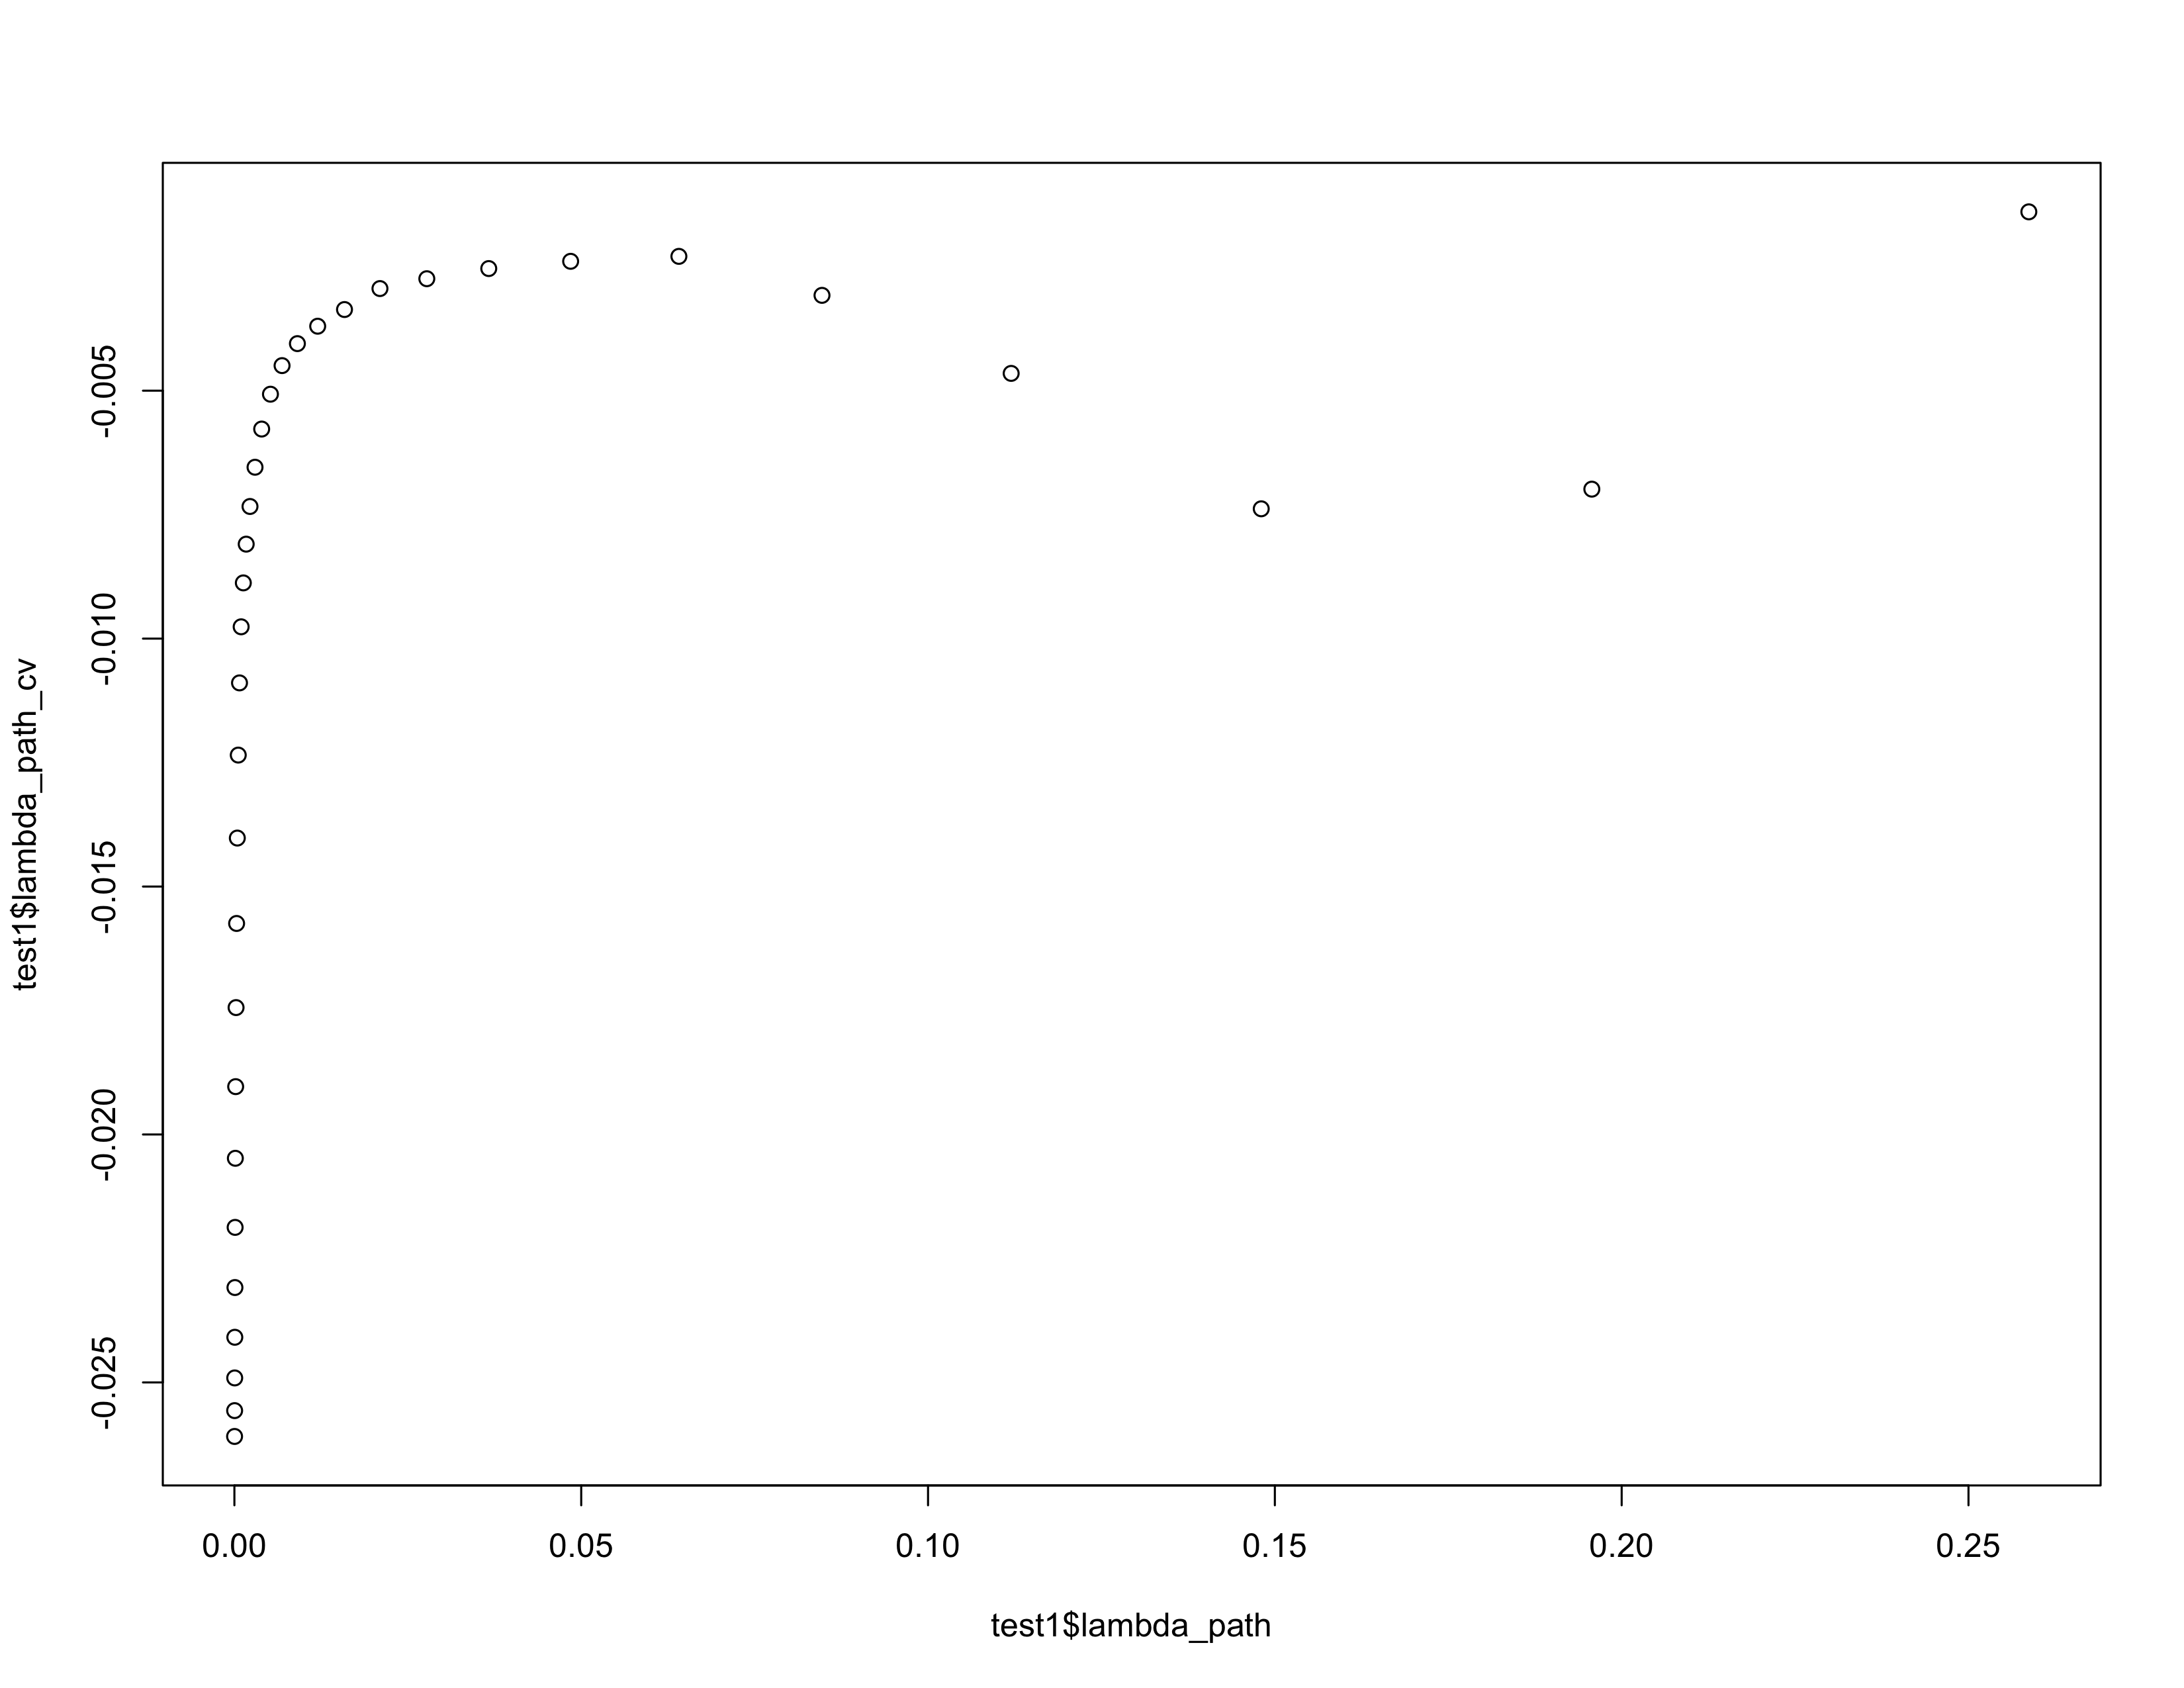
\includegraphics[width=1\linewidth]{./result_plot/correct/1_path_plot}
\end{subfigure}%
\begin{subfigure}{.5\textwidth}
  \centering
  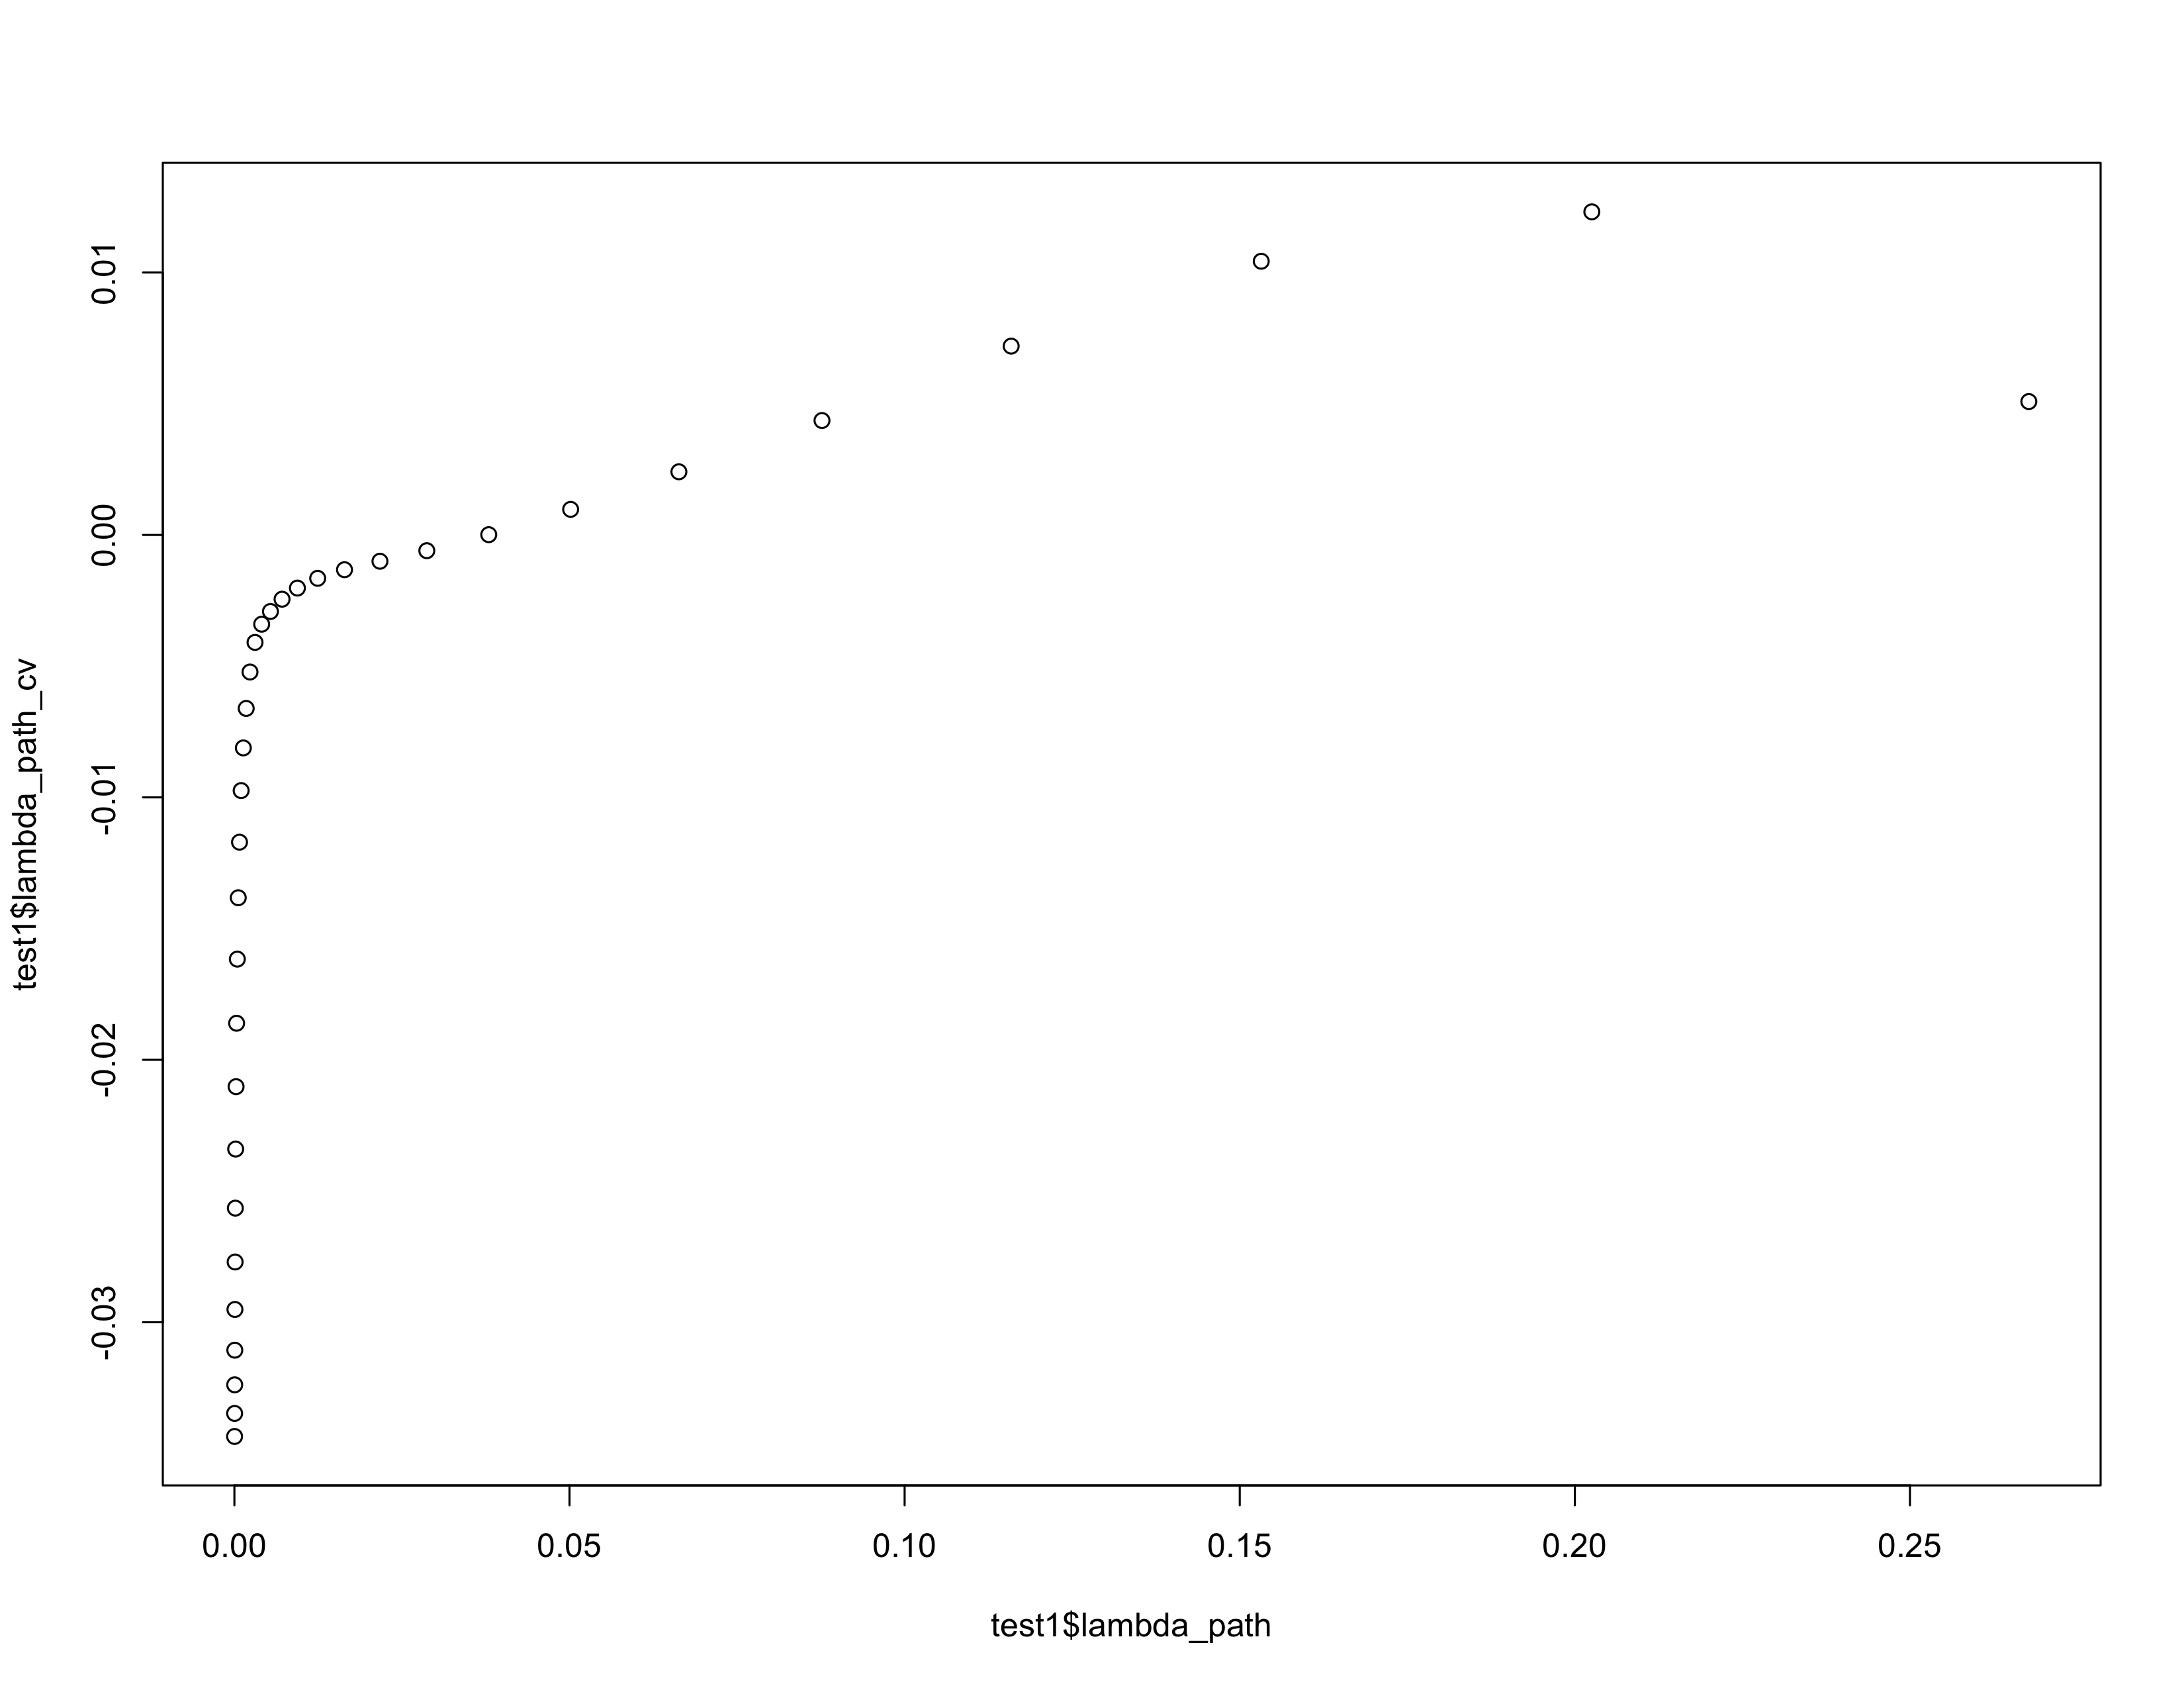
\includegraphics[width=1\linewidth]{./result_plot/correct/2_path_plot}
\end{subfigure}
\end{figure}

\begin{figure}[H]
\centering
\begin{subfigure}{0.5\textwidth}
  \centering
  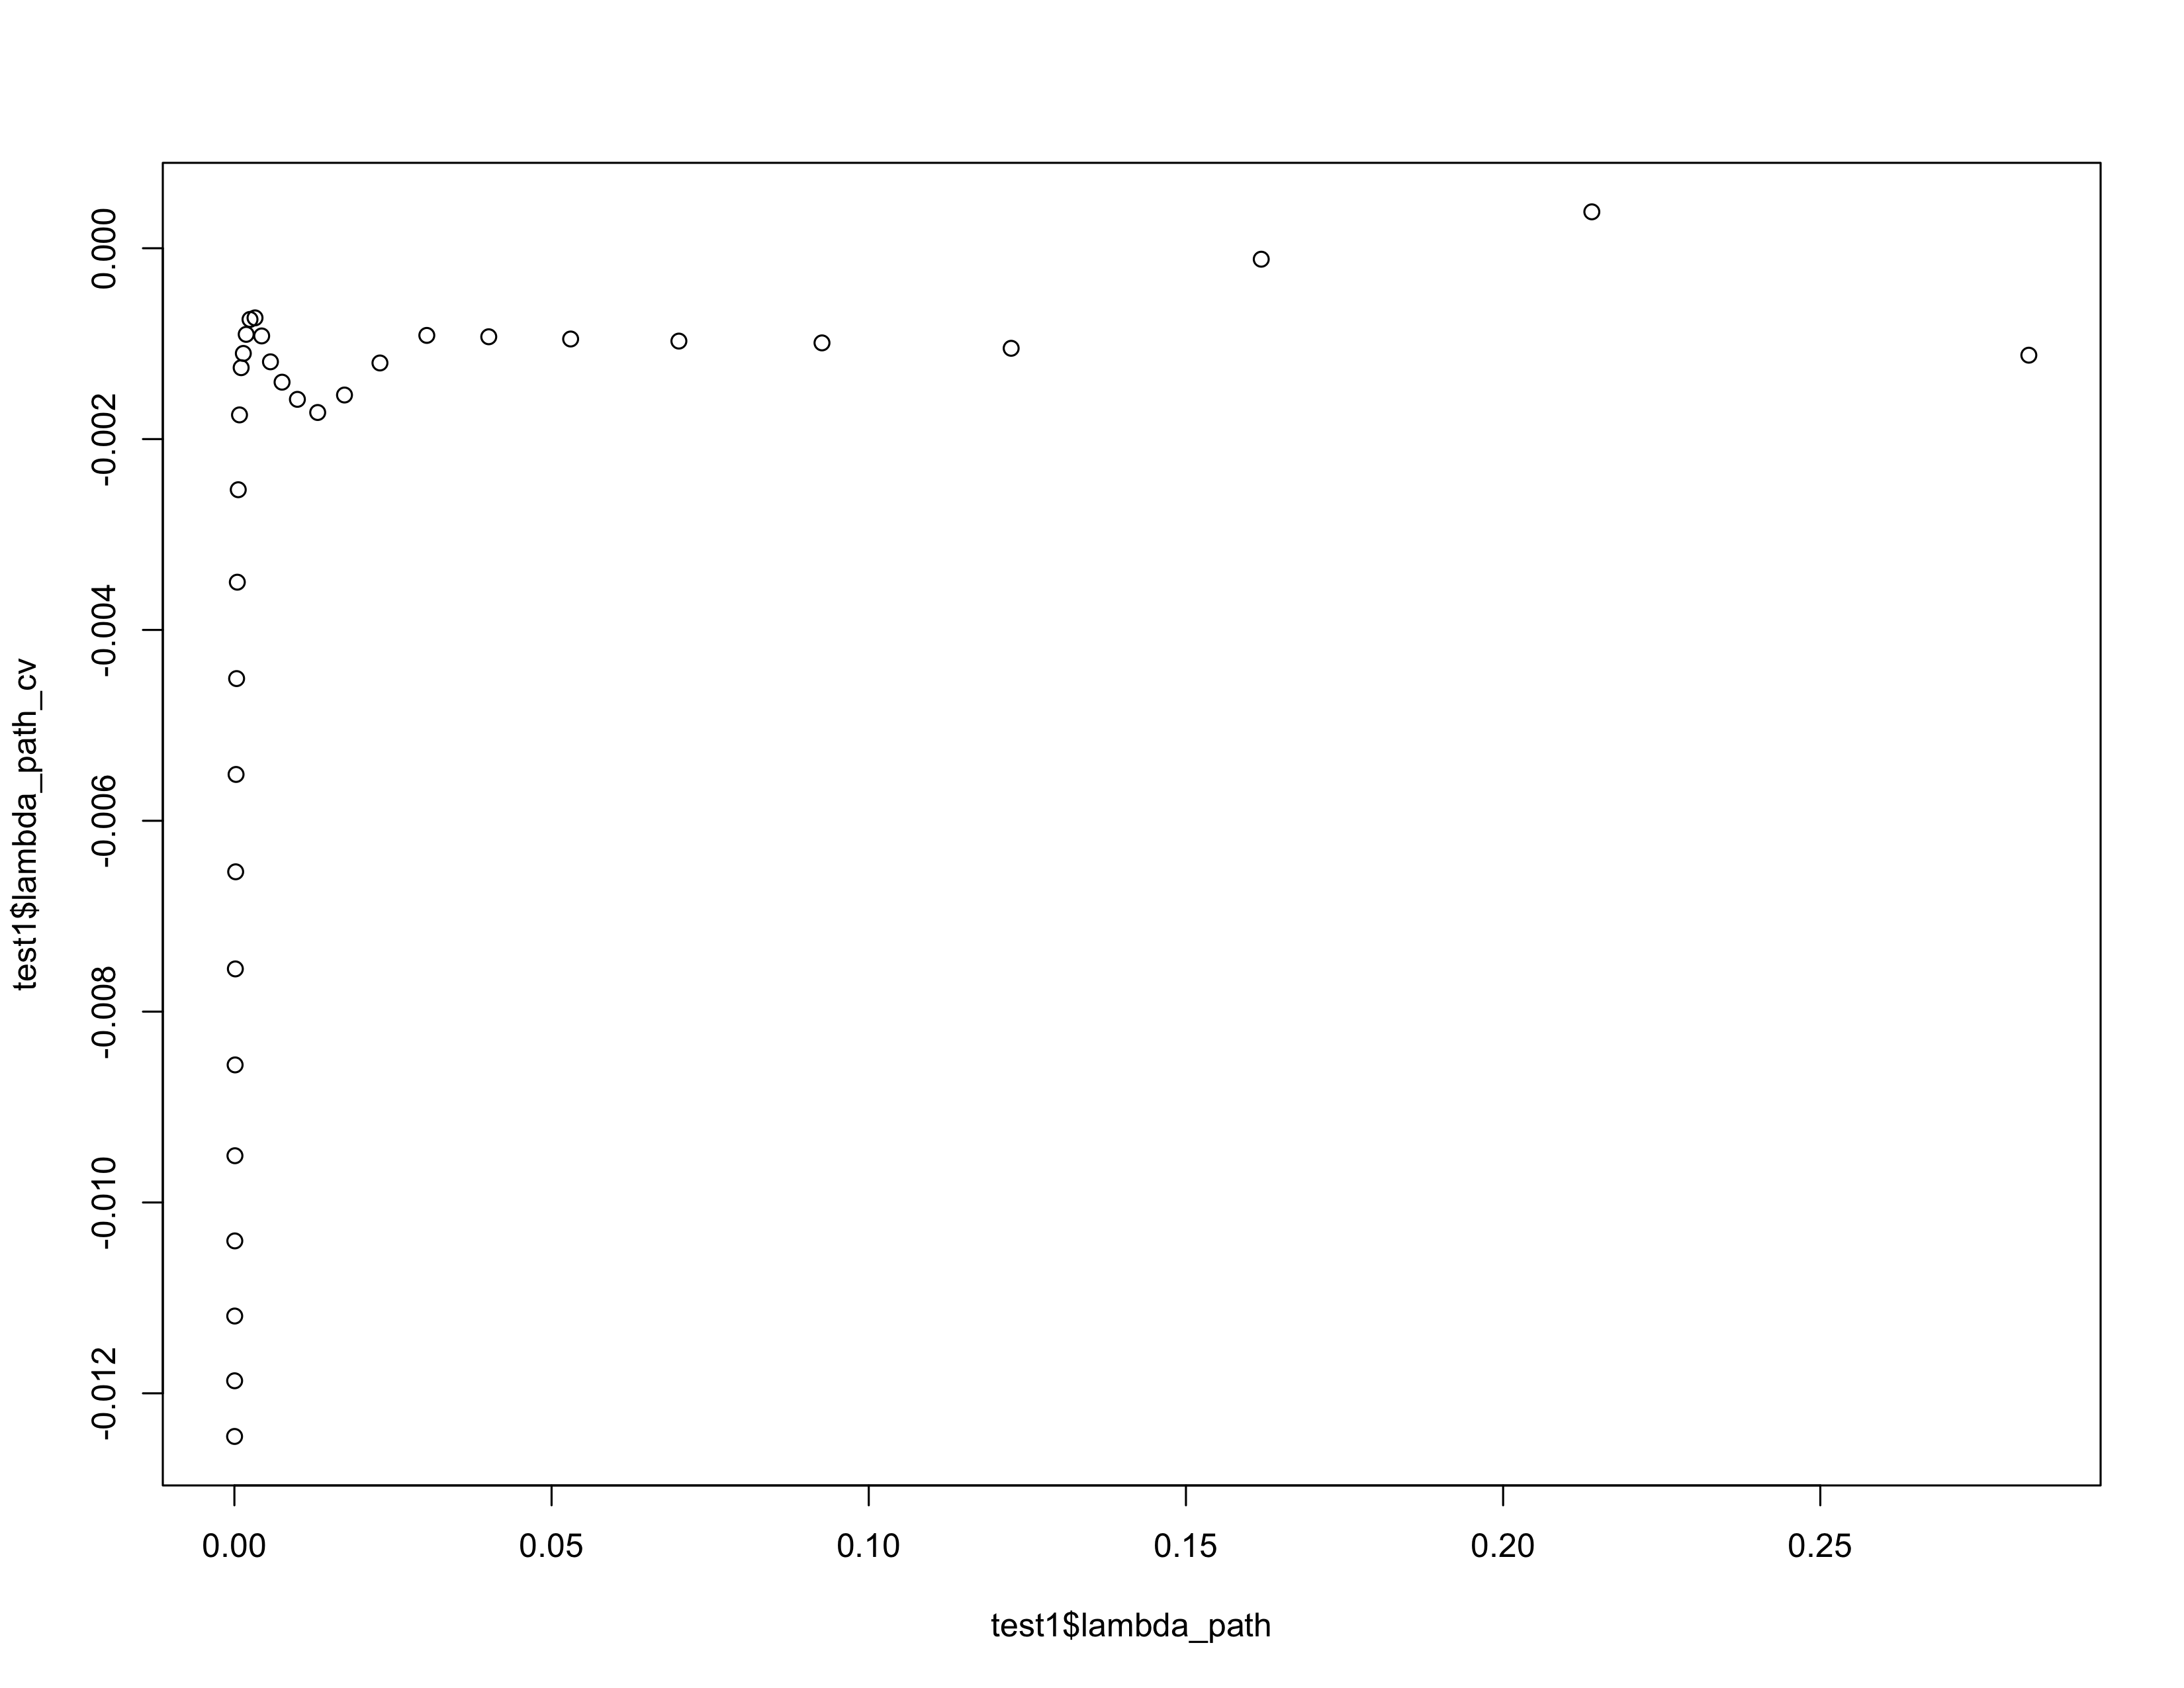
\includegraphics[width=1\linewidth]{./result_plot/correct/3_path_plot}
\end{subfigure}%
\begin{subfigure}{.5\textwidth}
  \centering
  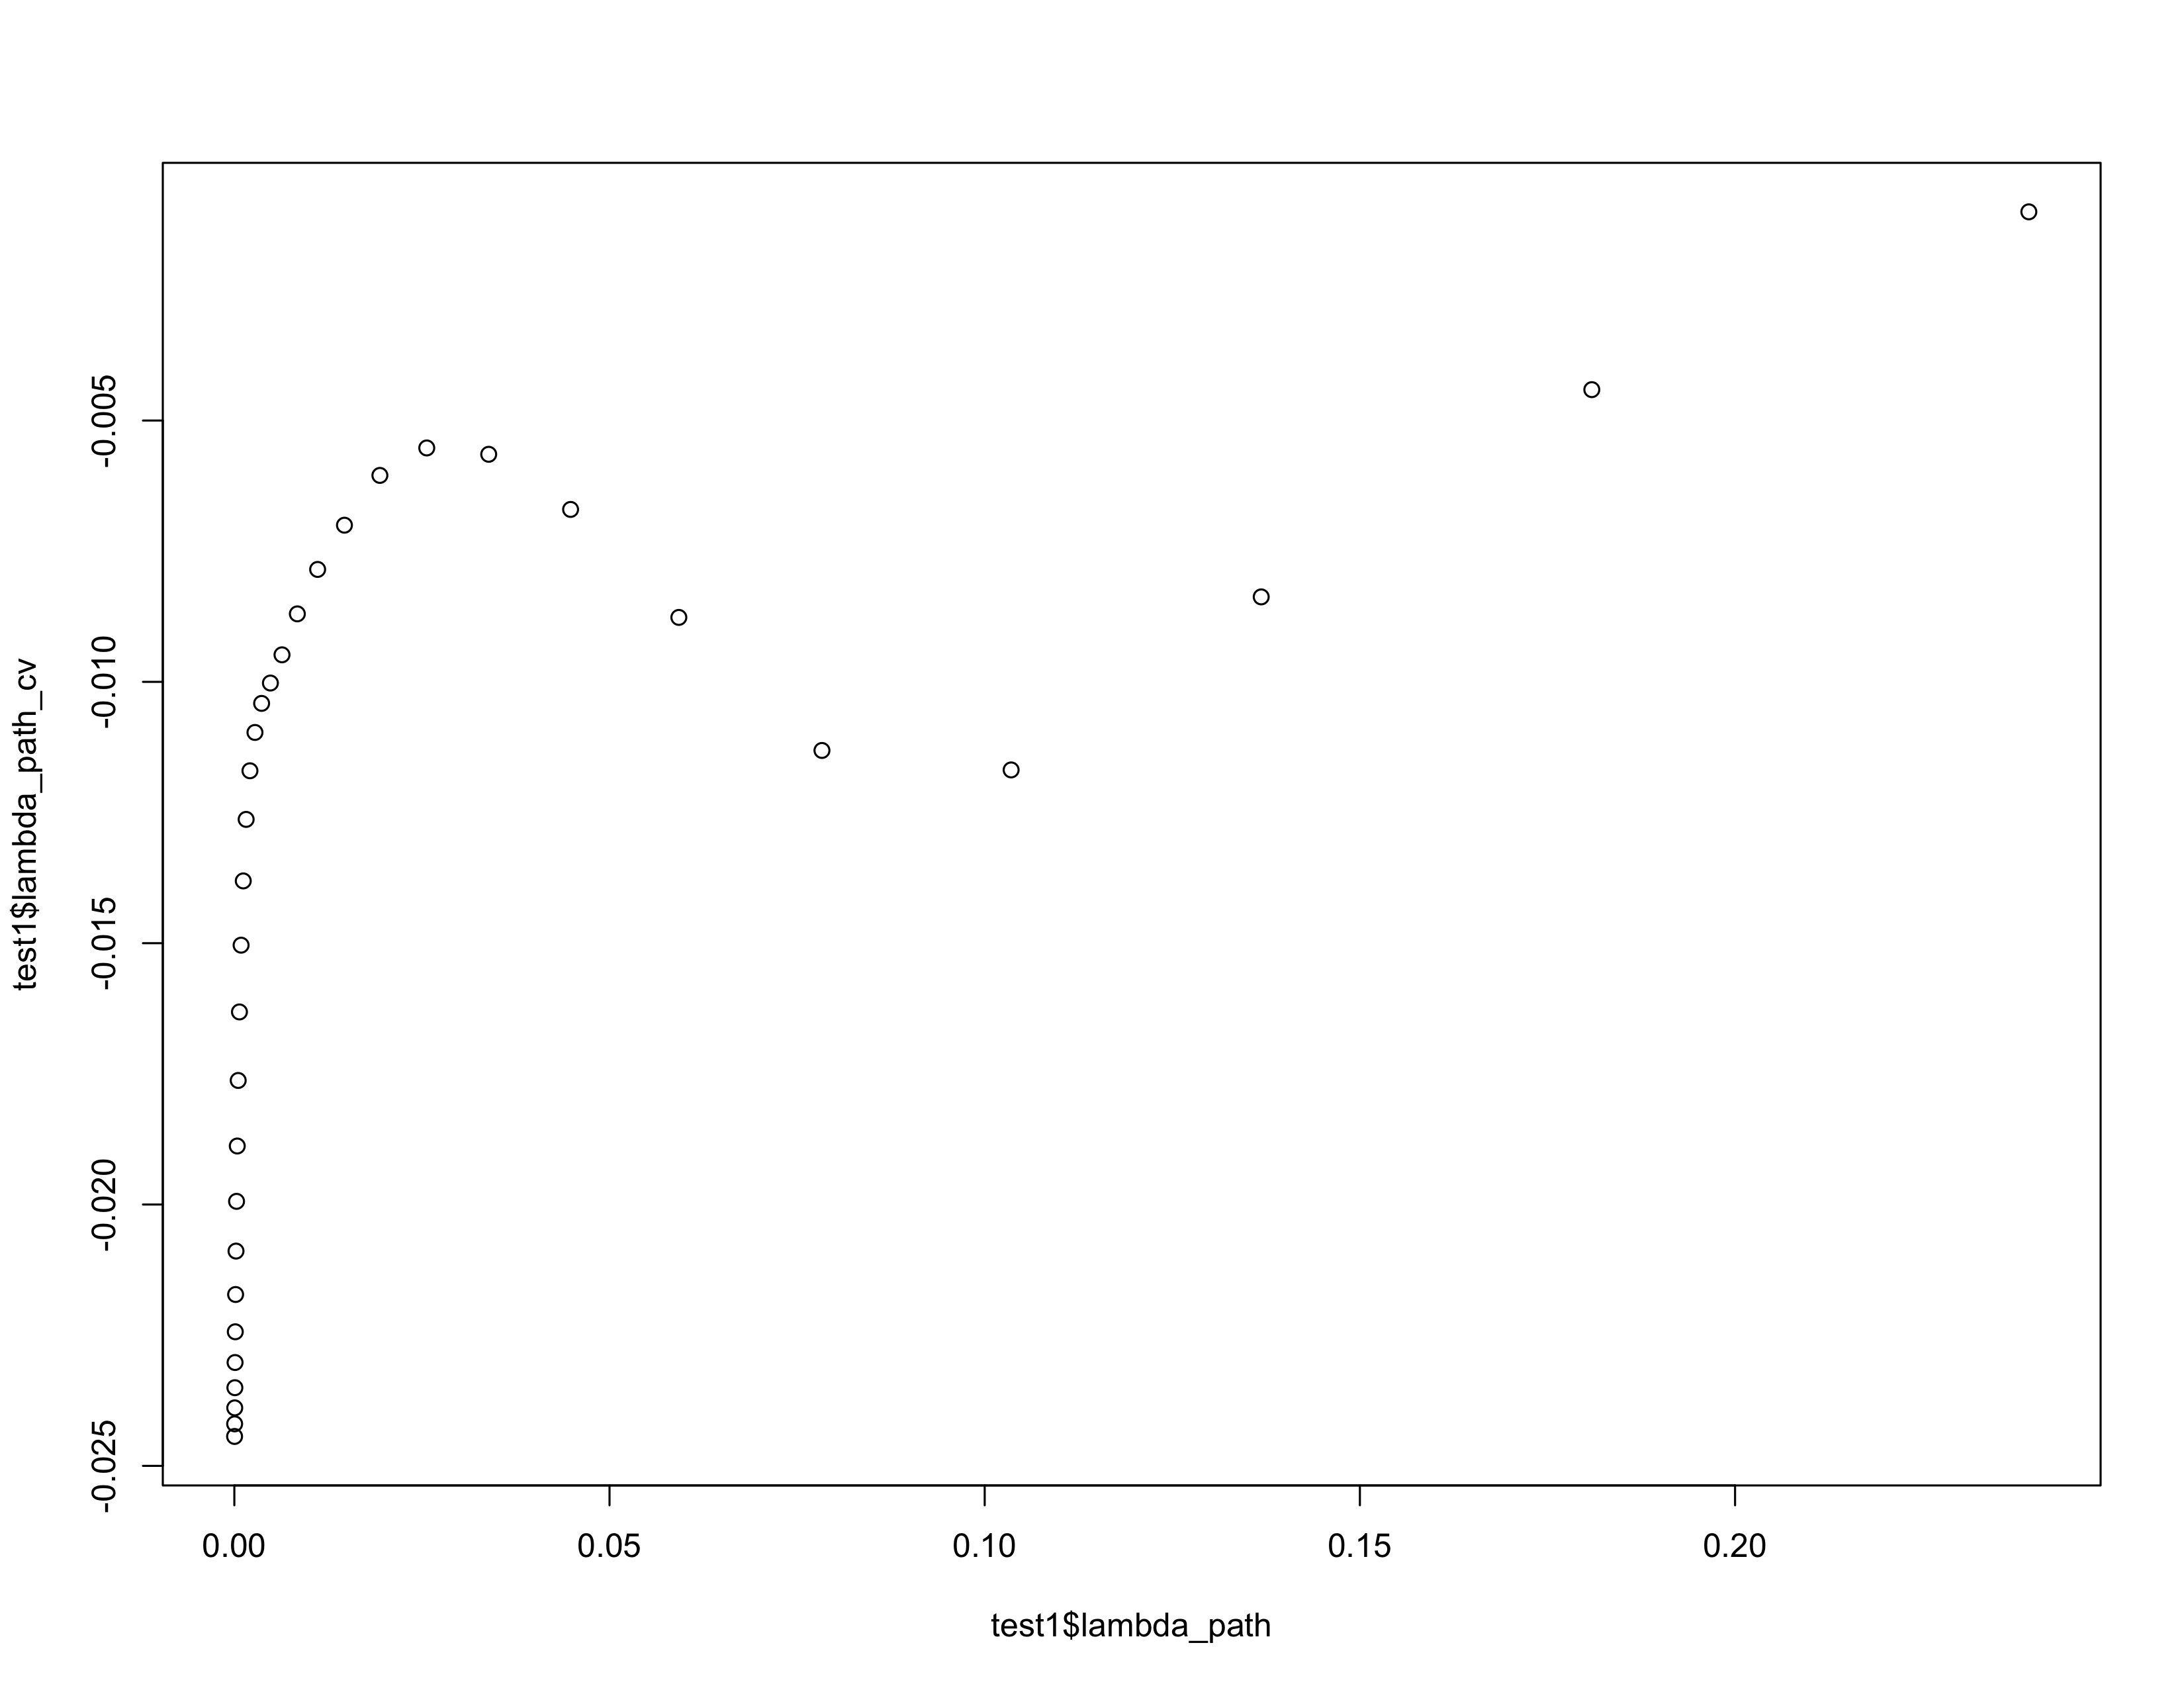
\includegraphics[width=1\linewidth]{./result_plot/correct/4_path_plot}
\end{subfigure}

\end{figure}

\begin{figure}[H]
\centering
\begin{subfigure}{0.5\textwidth}
  \centering
  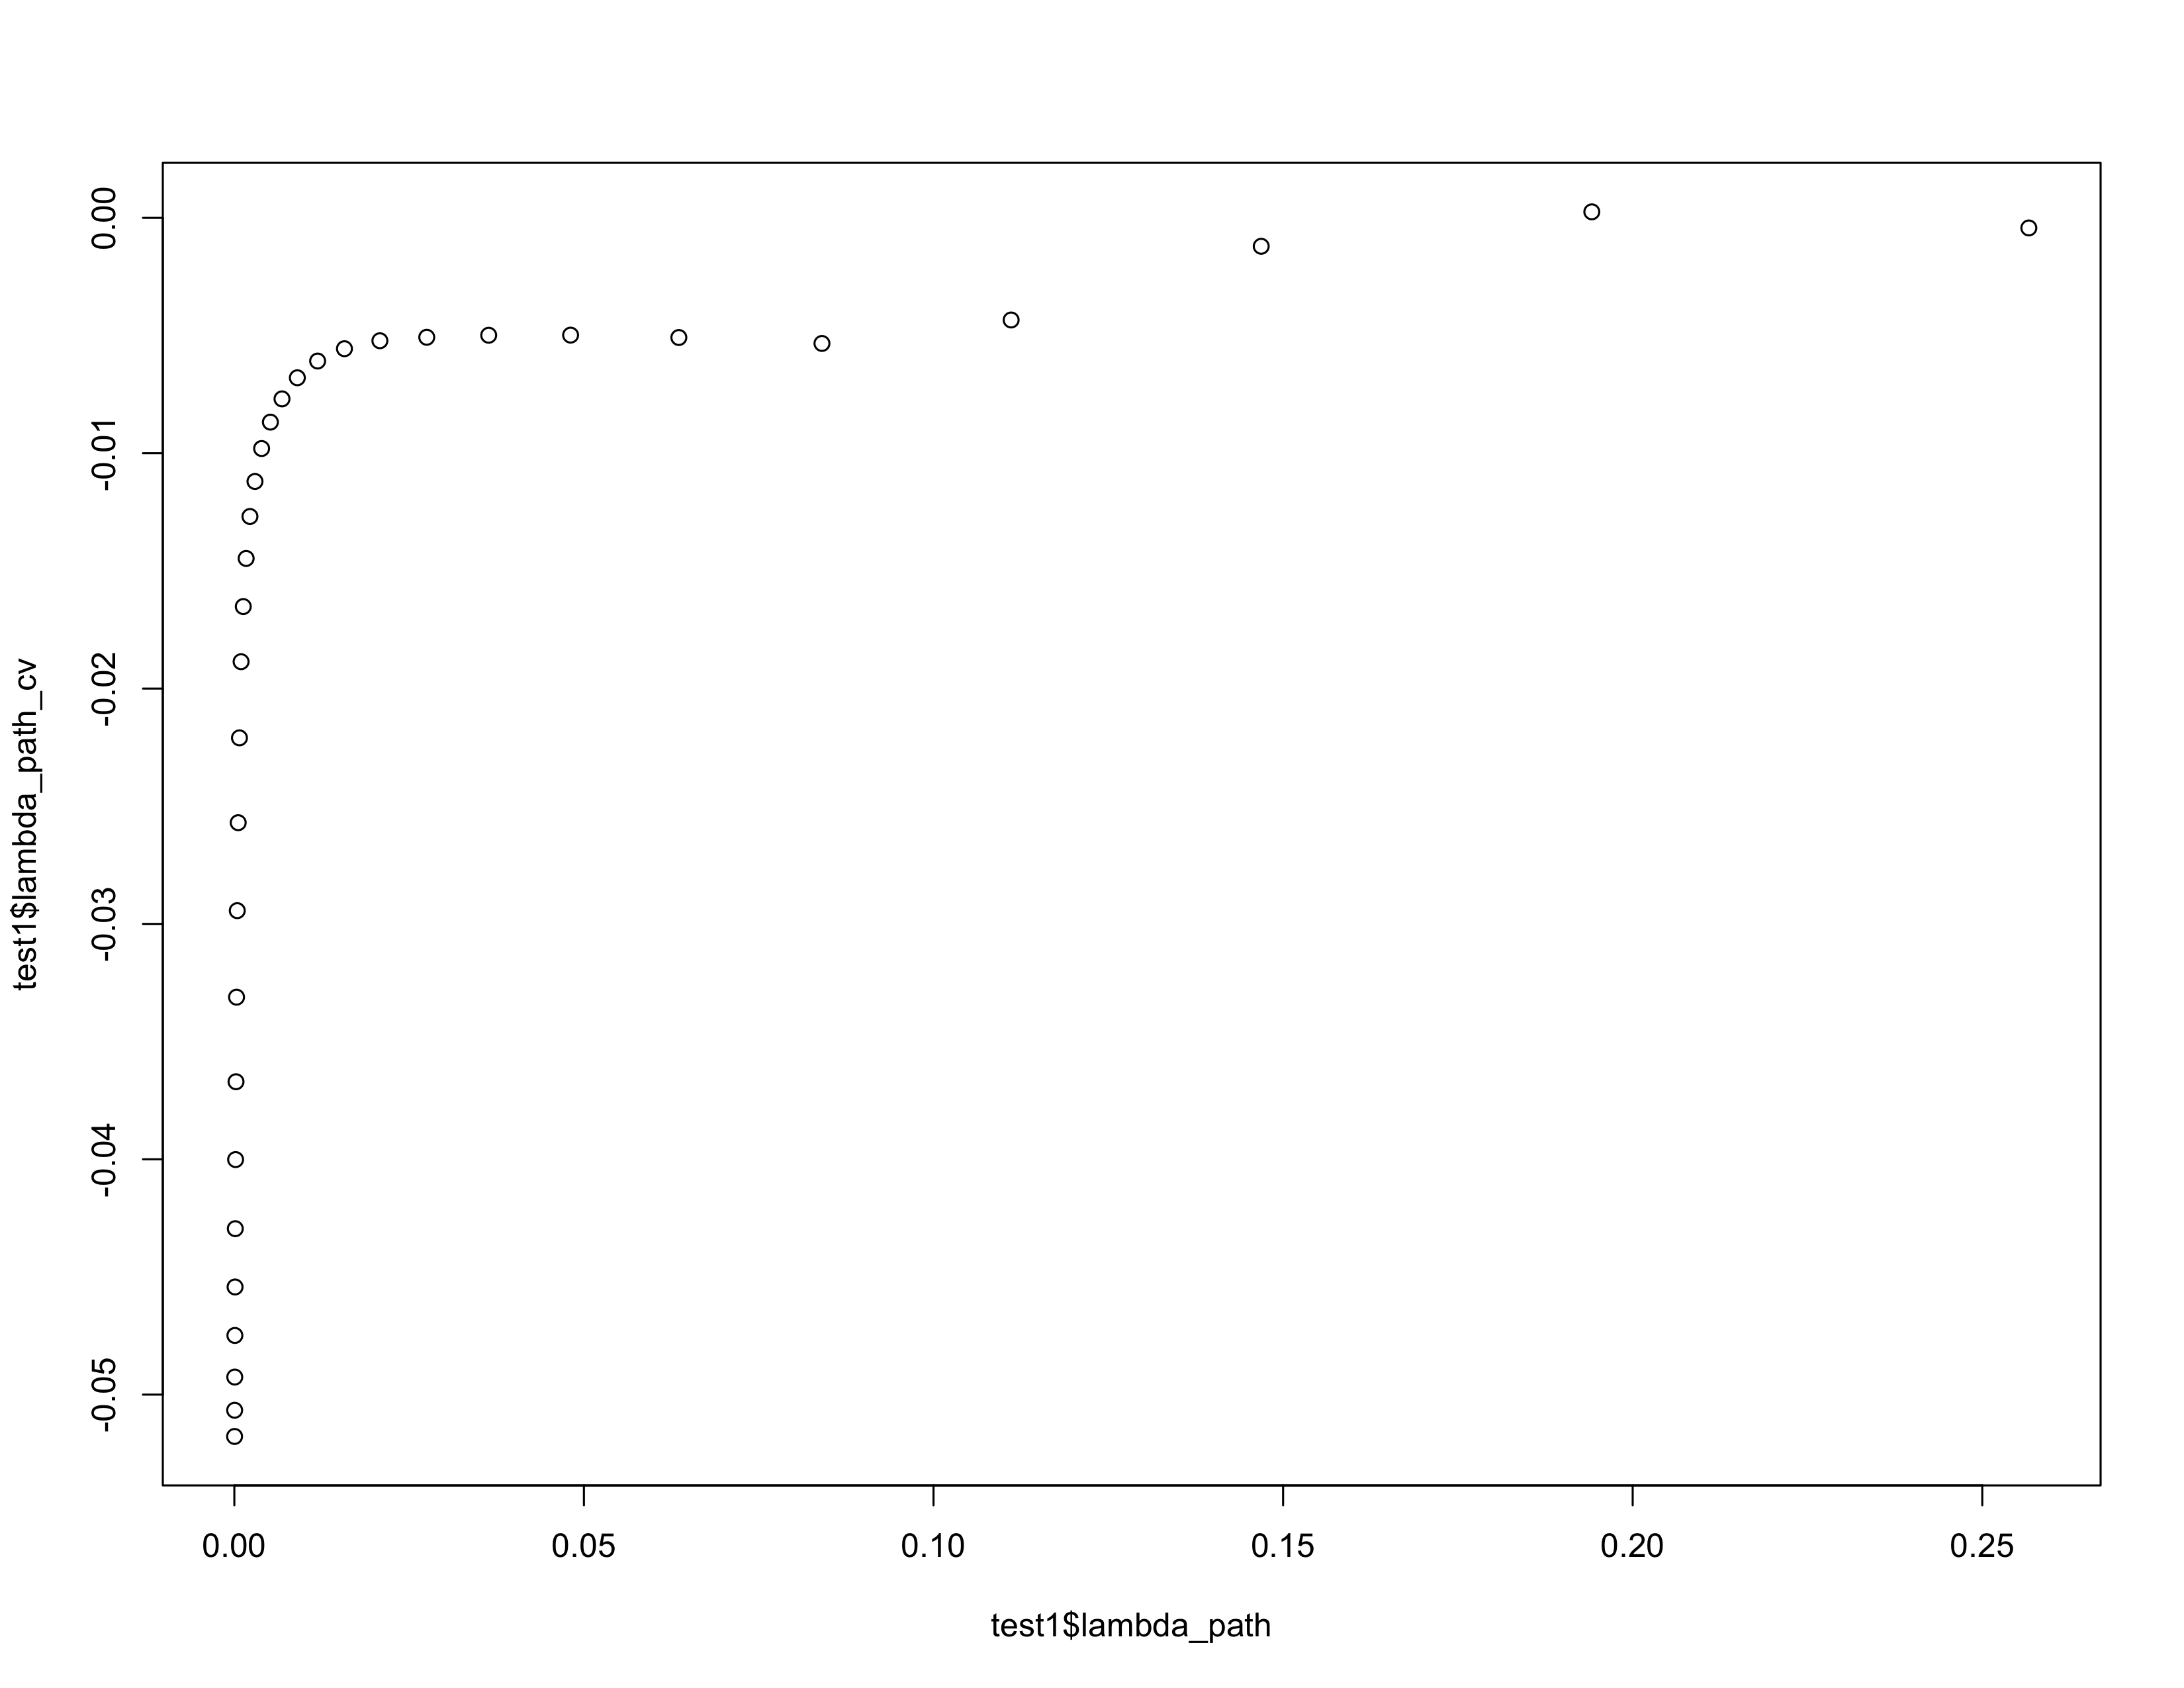
\includegraphics[width=1\linewidth]{./result_plot/correct/5_path_plot}
\end{subfigure}%
\begin{subfigure}{.5\textwidth}
  \centering
  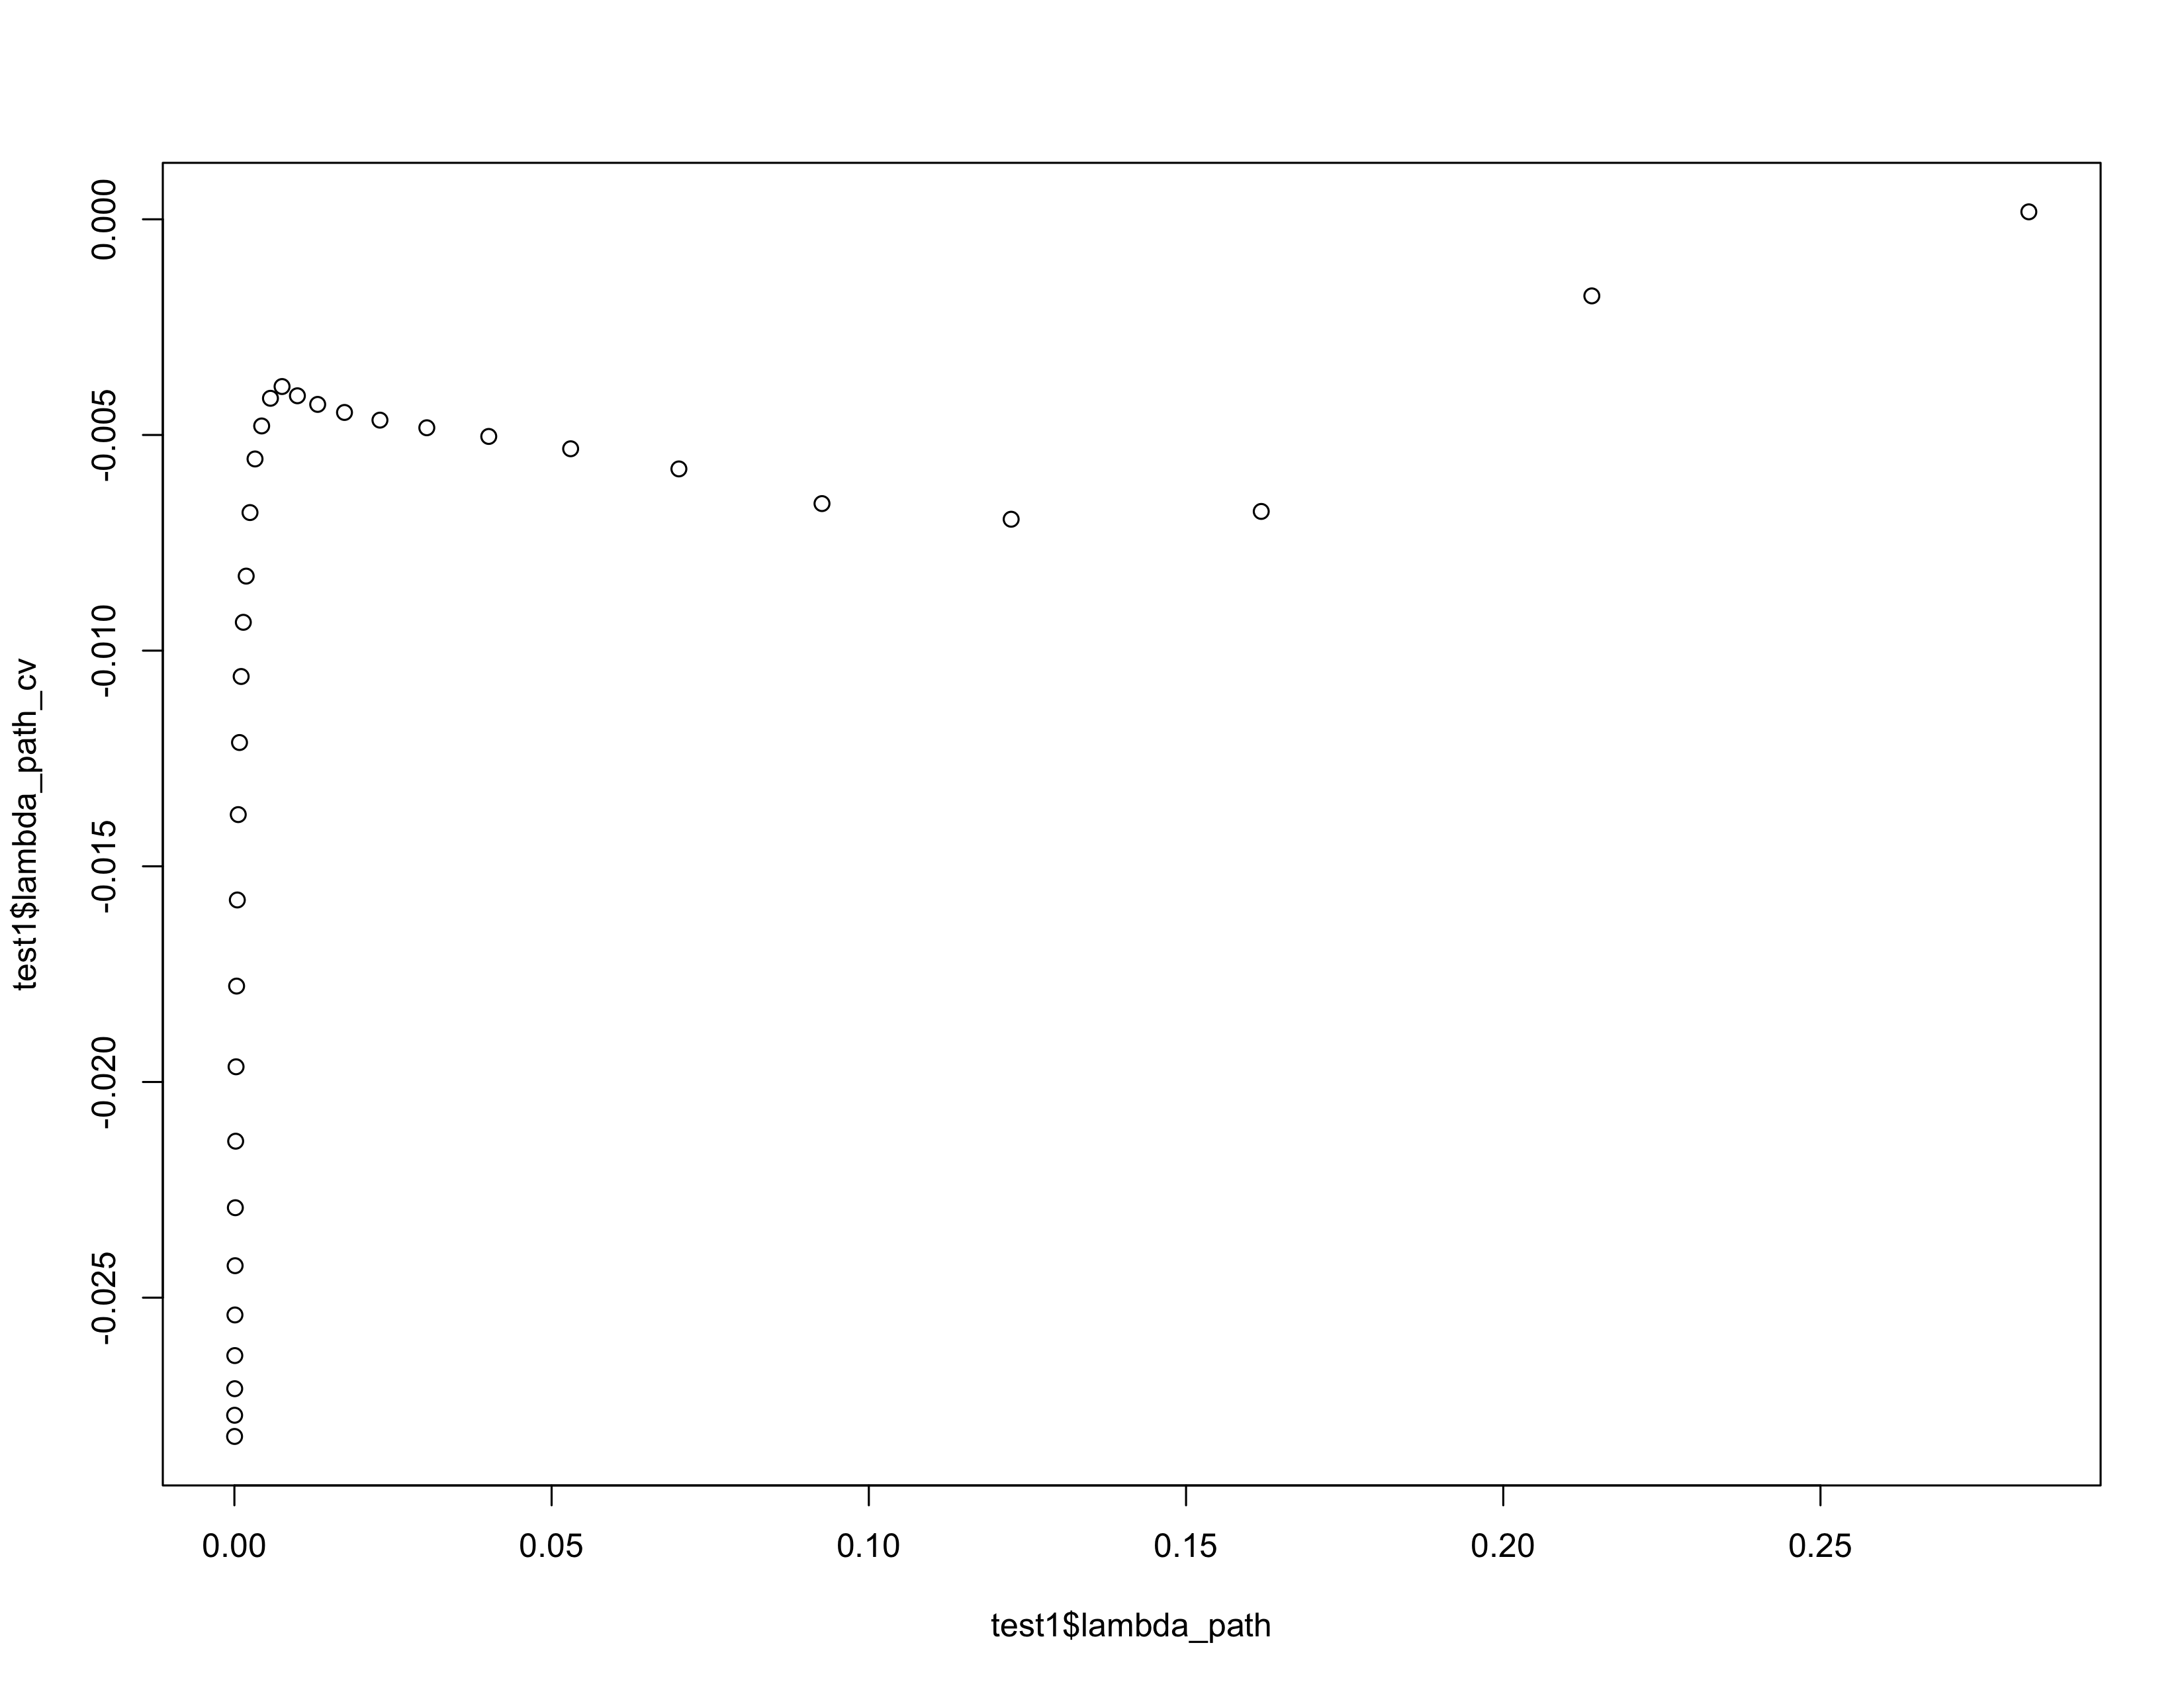
\includegraphics[width=1\linewidth]{./result_plot/correct/6_path_plot}
\end{subfigure}

\end{figure}

\begin{figure}[H]
\centering
\begin{subfigure}{0.5\textwidth}
  \centering
  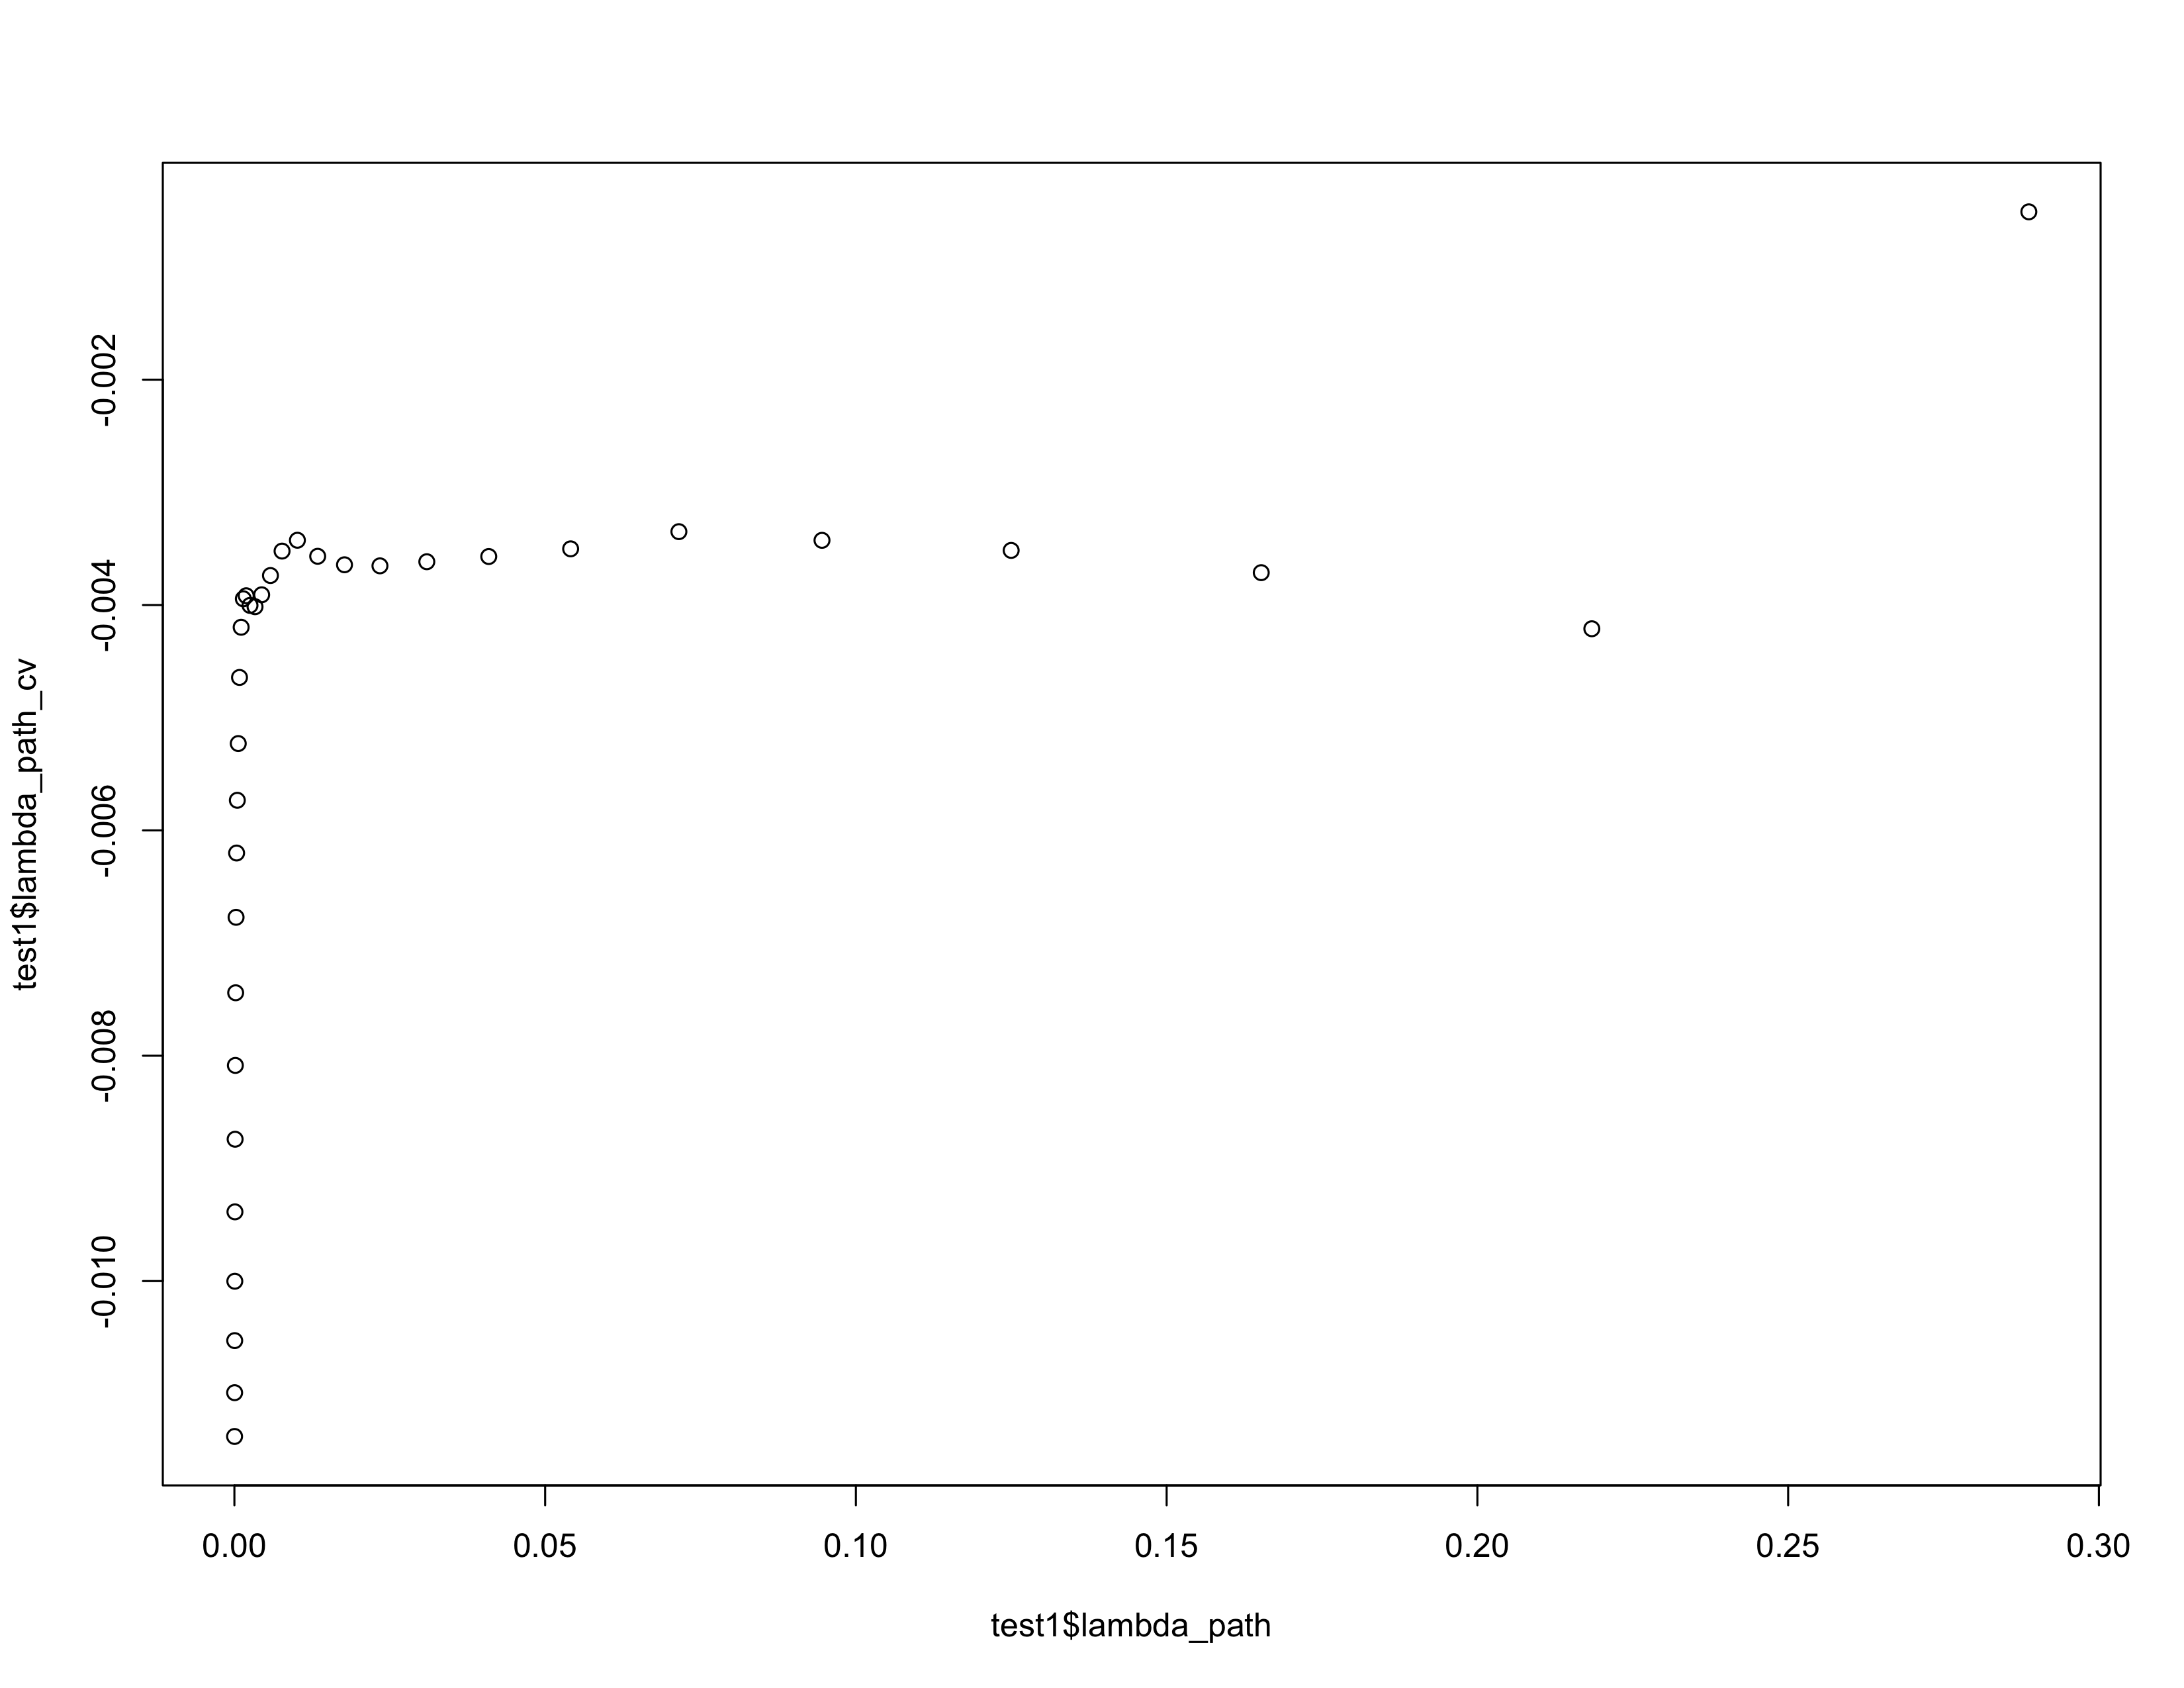
\includegraphics[width=1\linewidth]{./result_plot/correct/7_path_plot}
\end{subfigure}%
\begin{subfigure}{.5\textwidth}
  \centering
  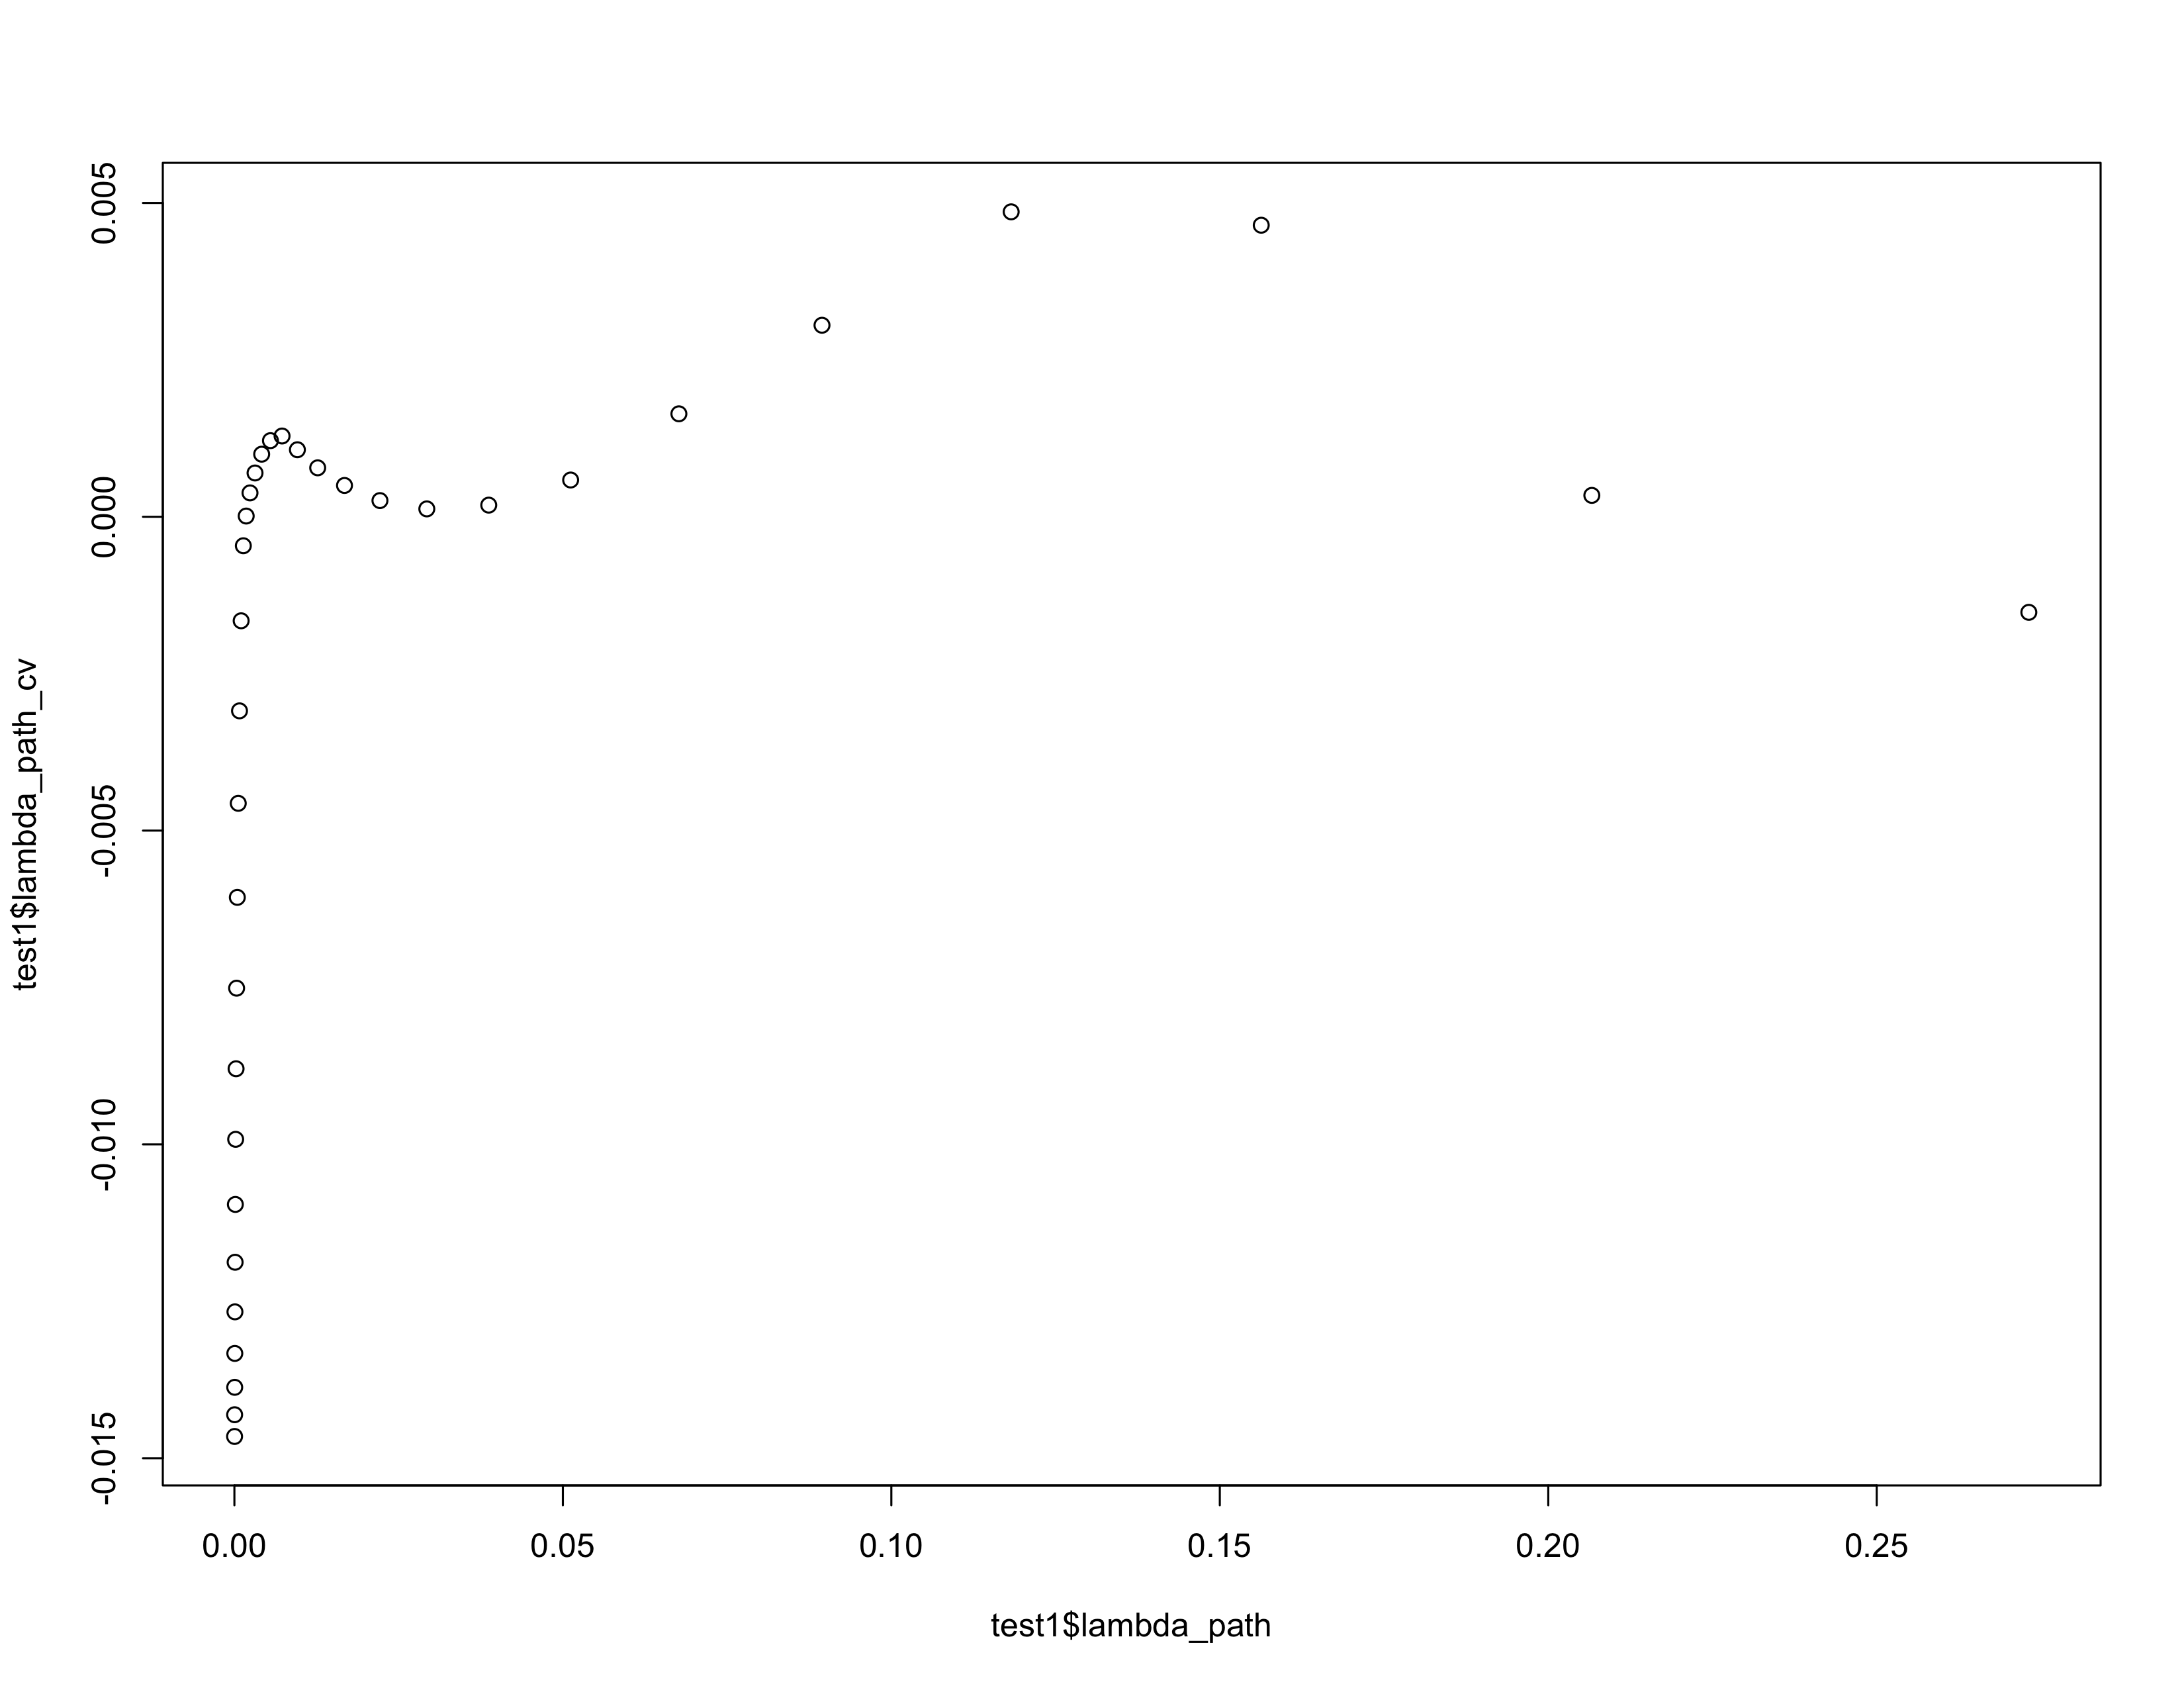
\includegraphics[width=1\linewidth]{./result_plot/correct/8_path_plot}
\end{subfigure}

\end{figure}

\begin{figure}[H]
\centering
\begin{subfigure}{0.5\textwidth}
  \centering
  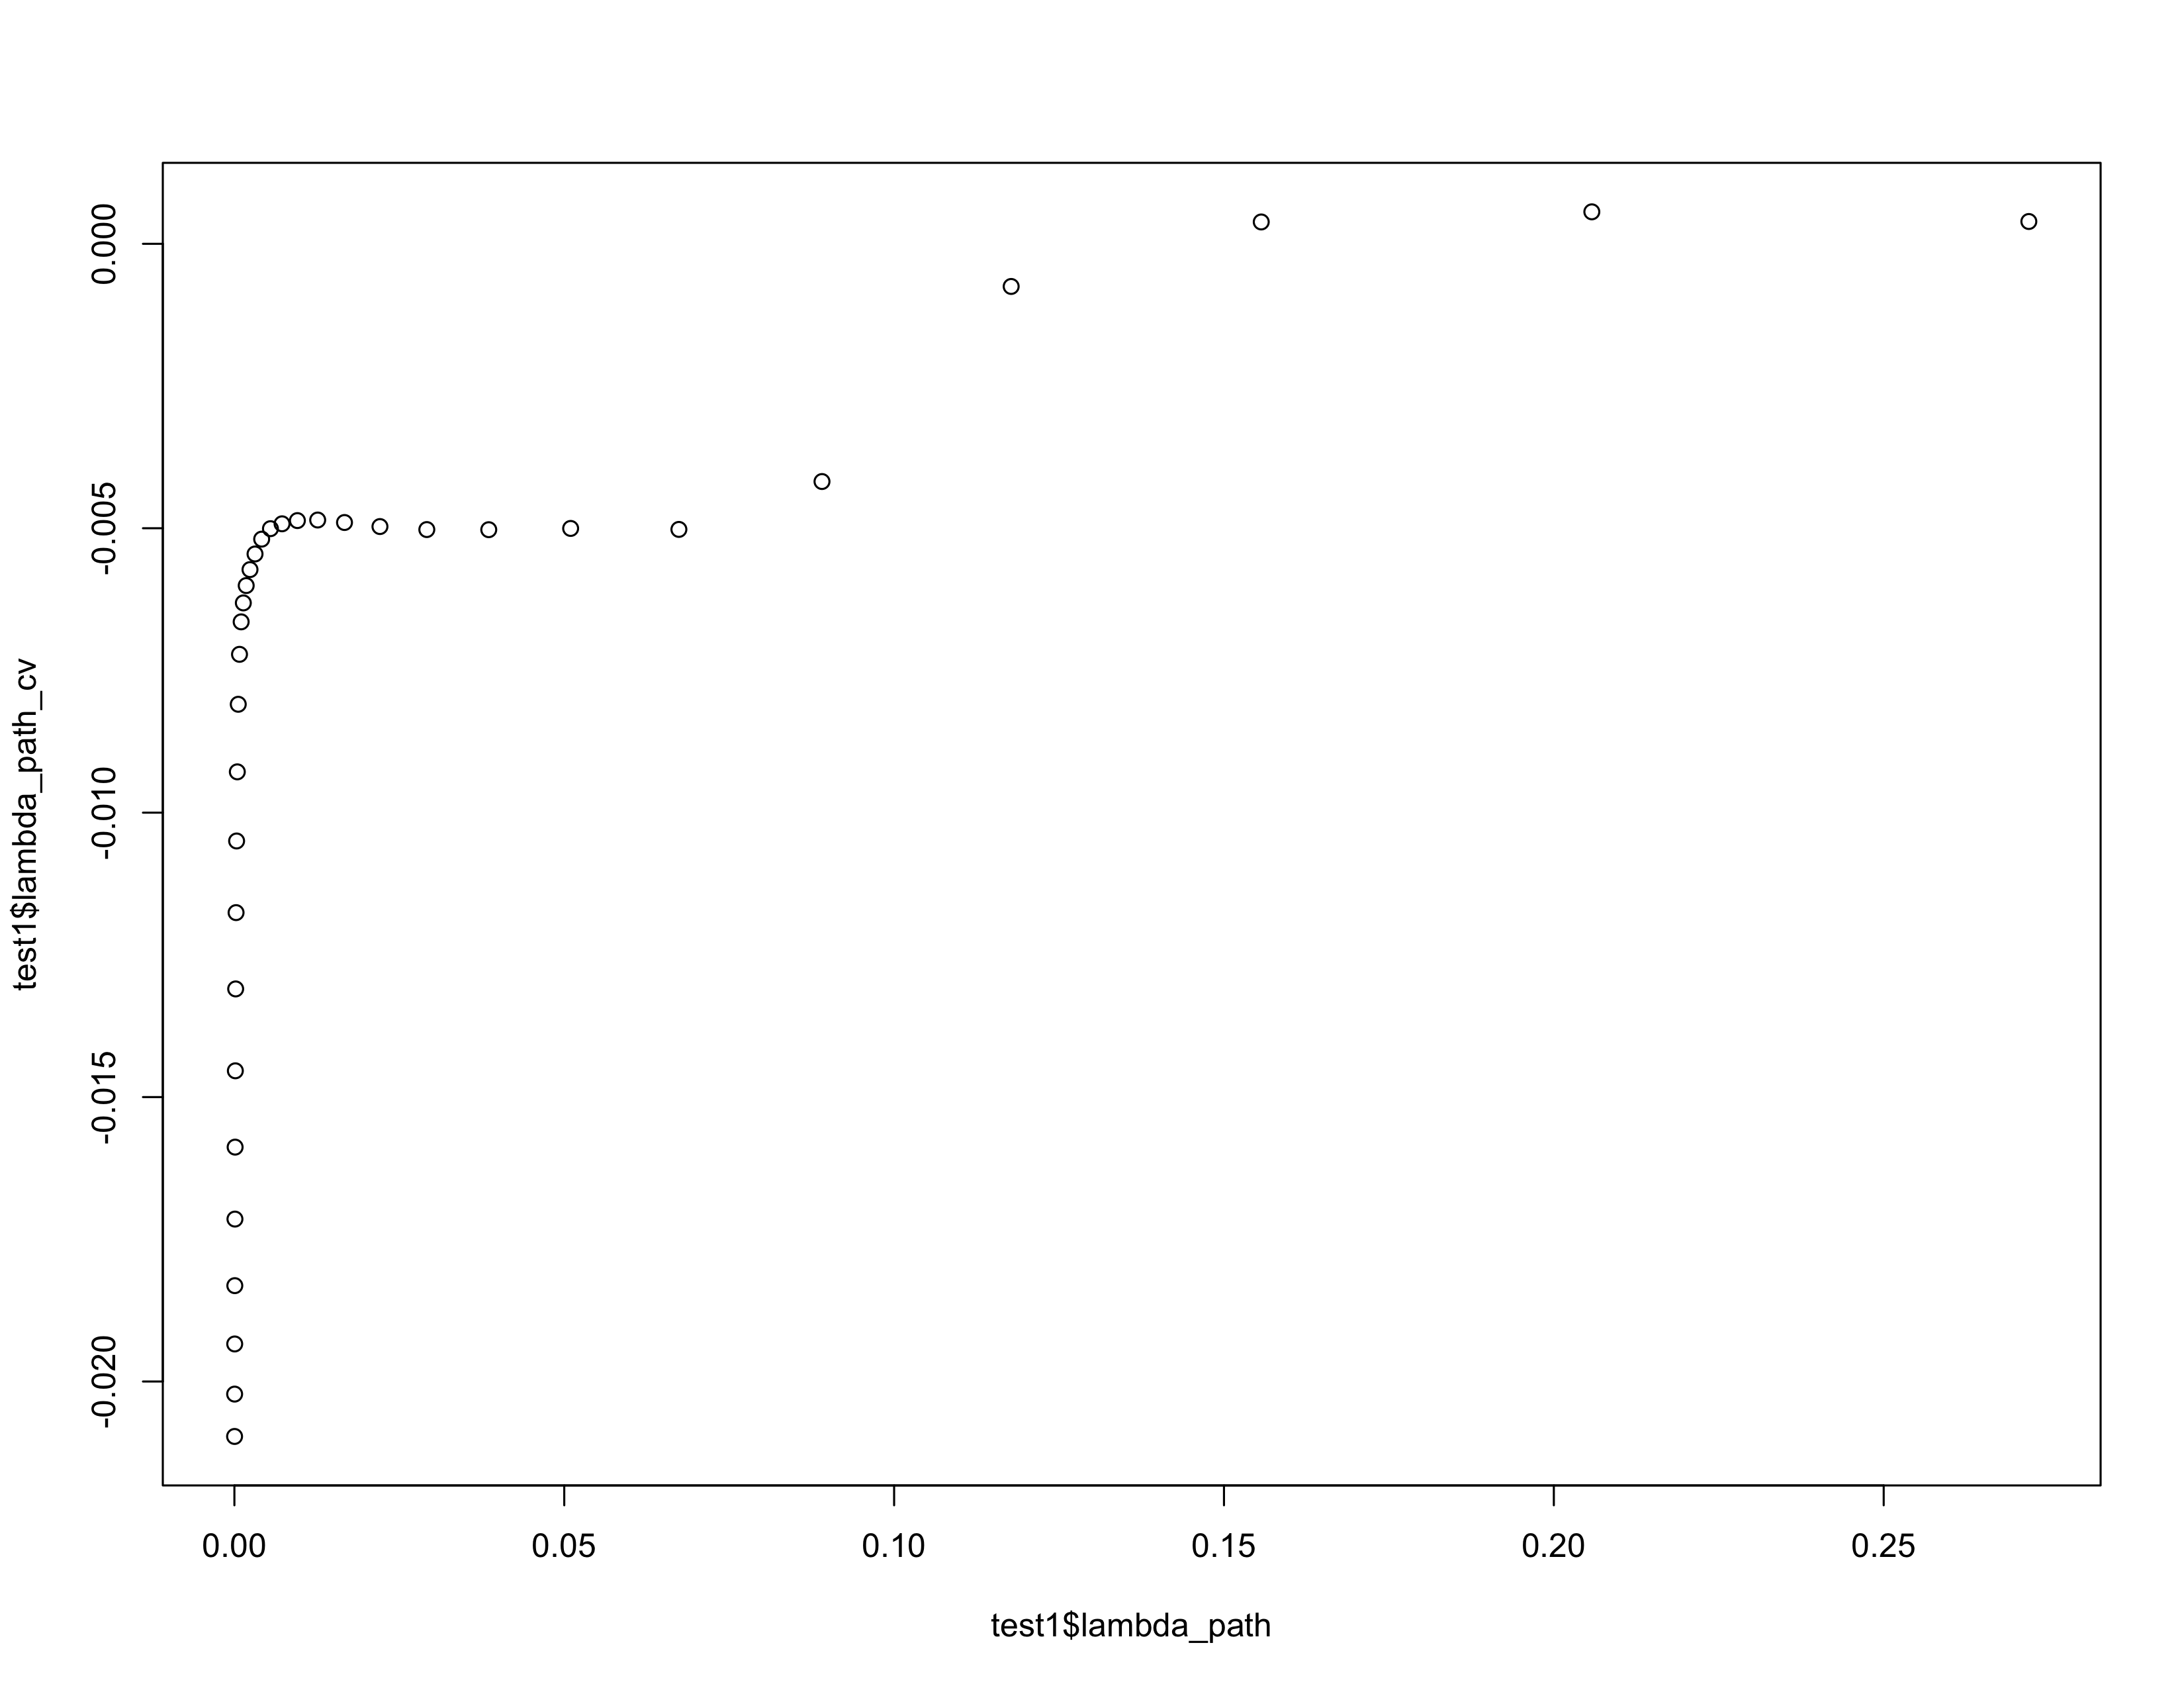
\includegraphics[width=1\linewidth]{./result_plot/correct/9_path_plot}
\end{subfigure}%
\begin{subfigure}{.5\textwidth}
  \centering
  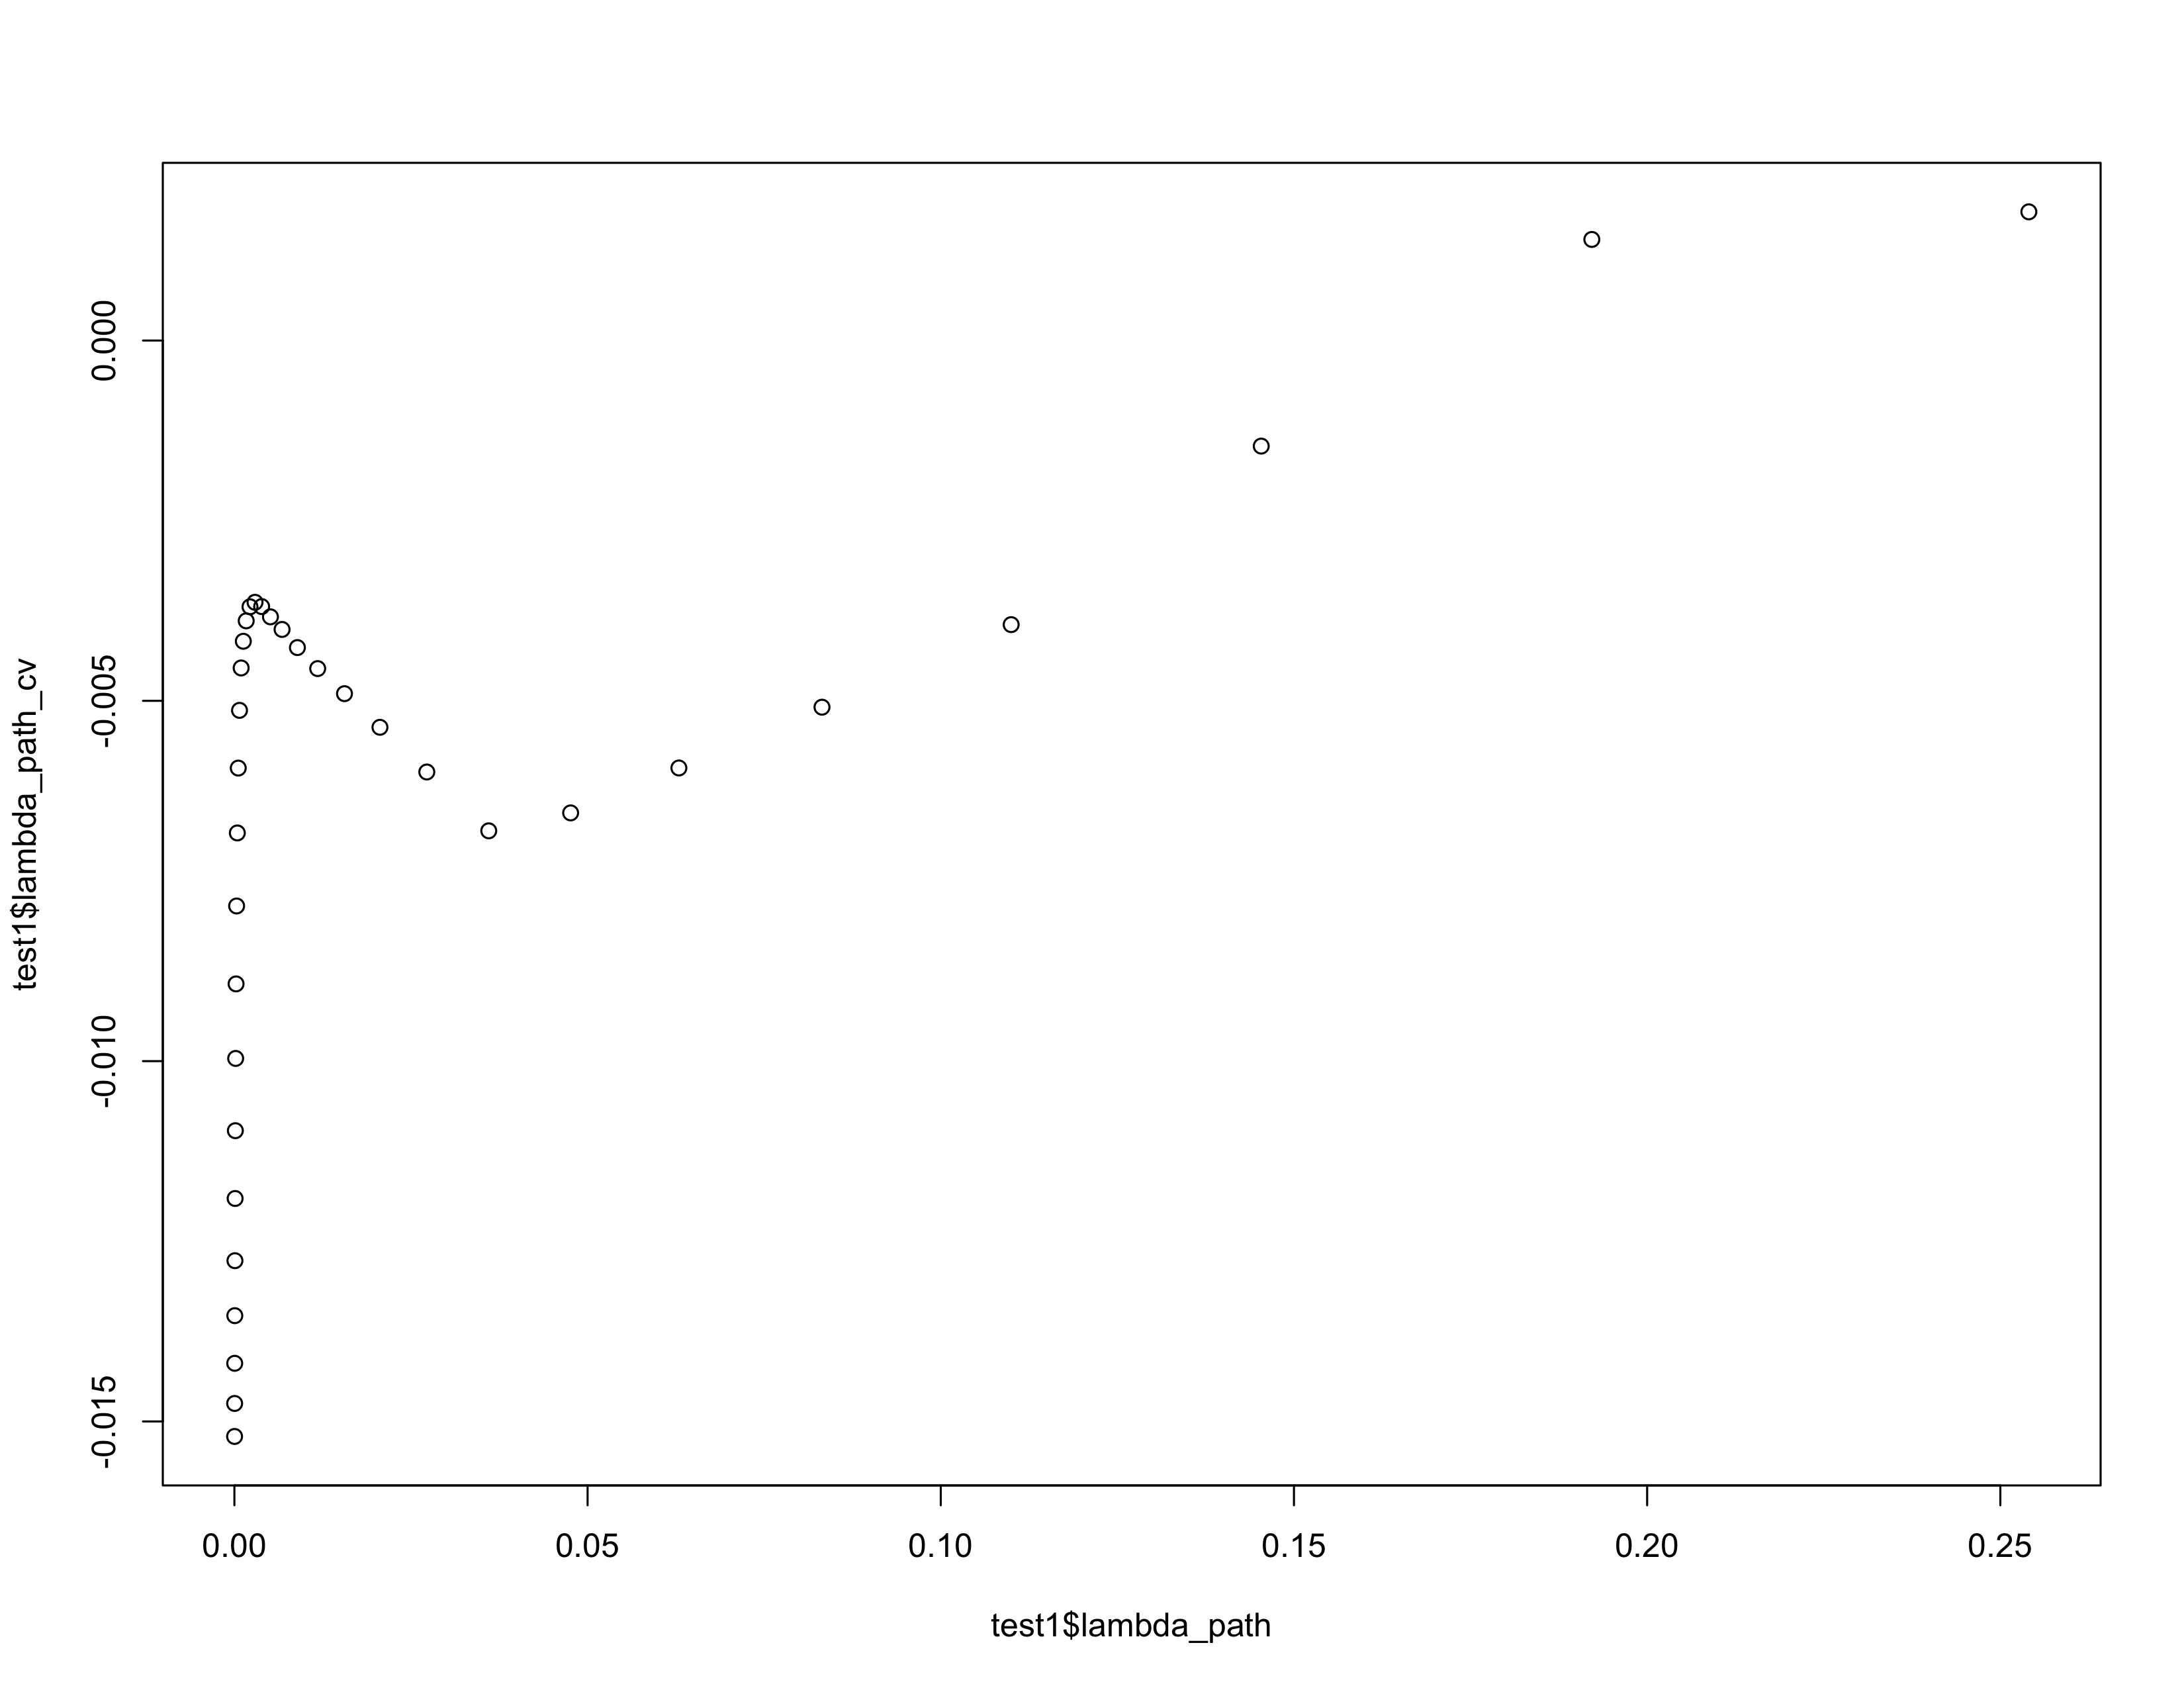
\includegraphics[width=1\linewidth]{./result_plot/correct/10_path_plot}
\end{subfigure}

\end{figure}

\section{wrong index}
\label{sec:wrong}
This is the wrong thing I did in last time in our meeting.
Only when $k=5$ has been counted to our $\text{cv}(\lambda)$.
In this section, we define:
$$
\argmin_{\lambda}\text{cv}(\lambda)=\argmin_{\lambda}\{l(\hat{\beta}_\lambda^{(-k)})-l^{(-k)}\hat{\beta}_(\lambda^{(-k)})\}
$$,
where $\text{k} = 5$
The plots we got are

\begin{figure}[H]
\centering
\begin{subfigure}{0.5\textwidth}
  \centering
  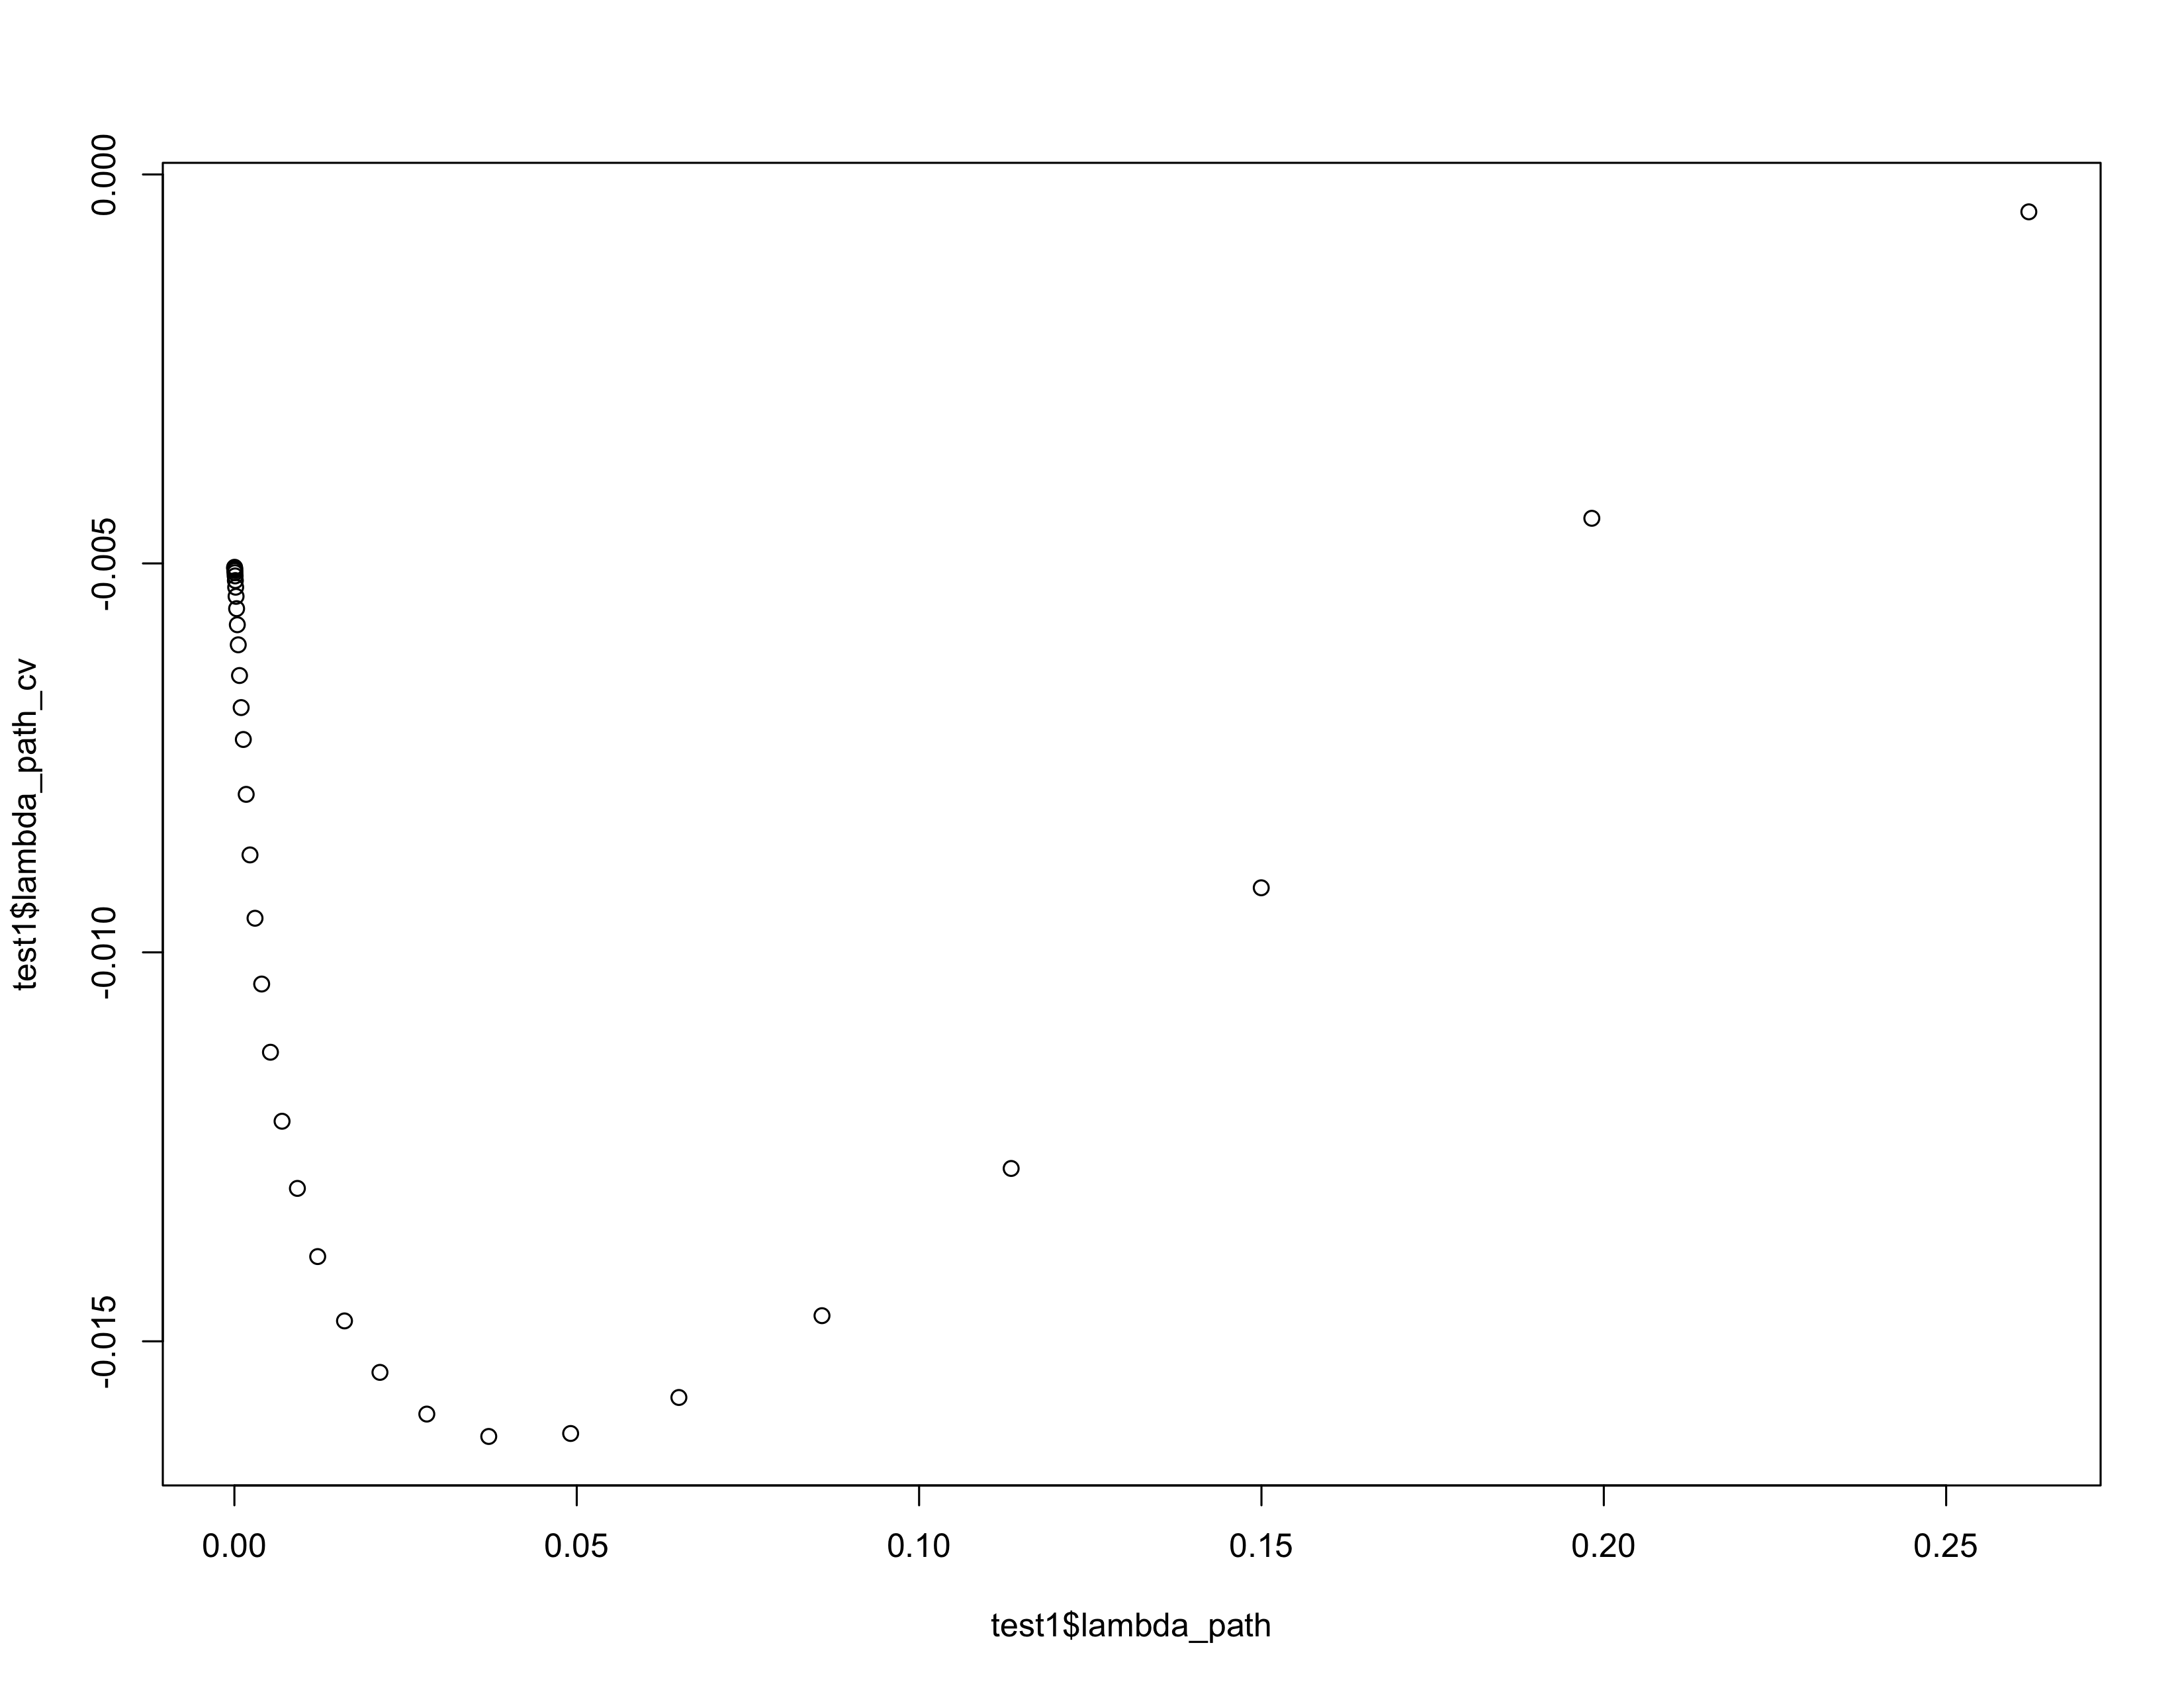
\includegraphics[width=1\linewidth]{./result_plot/fix_k/1wrong_path_plot}
\end{subfigure}%
\begin{subfigure}{.5\textwidth}
  \centering
  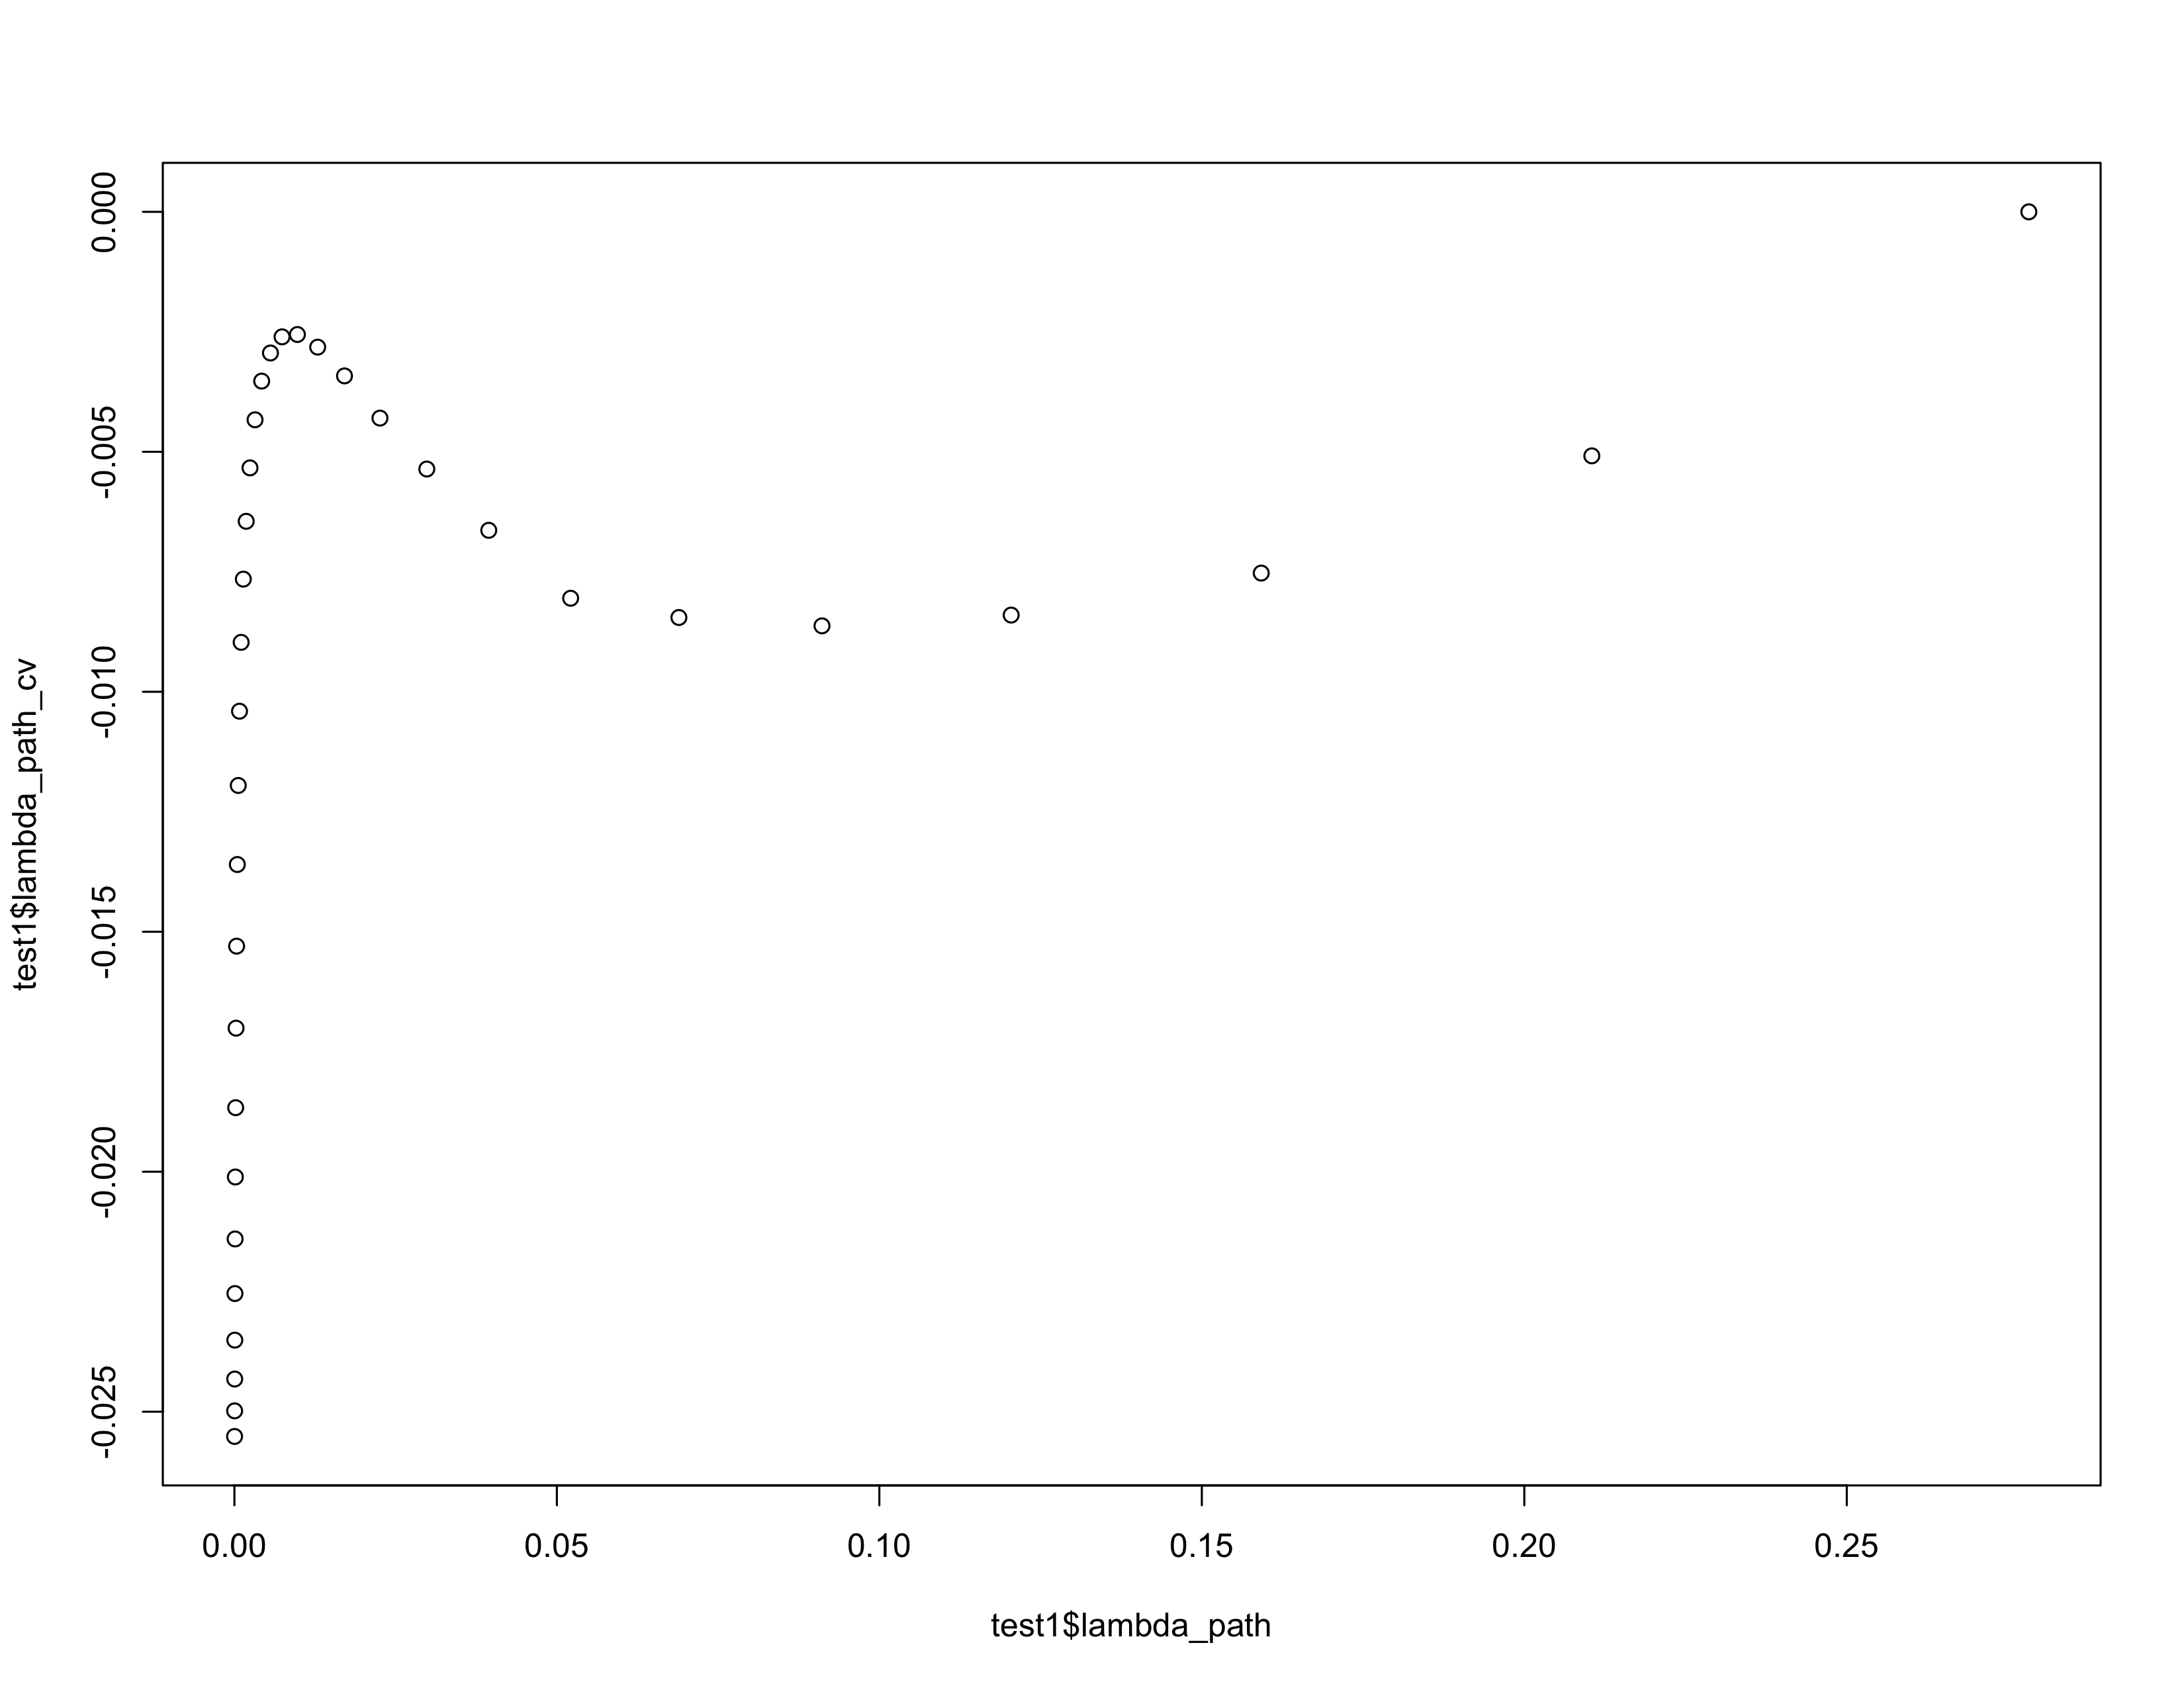
\includegraphics[width=1\linewidth]{./result_plot/fix_k/2wrong_path_plot}
\end{subfigure}

\end{figure}

\begin{figure}[H]
\centering
\begin{subfigure}{0.5\textwidth}
  \centering
  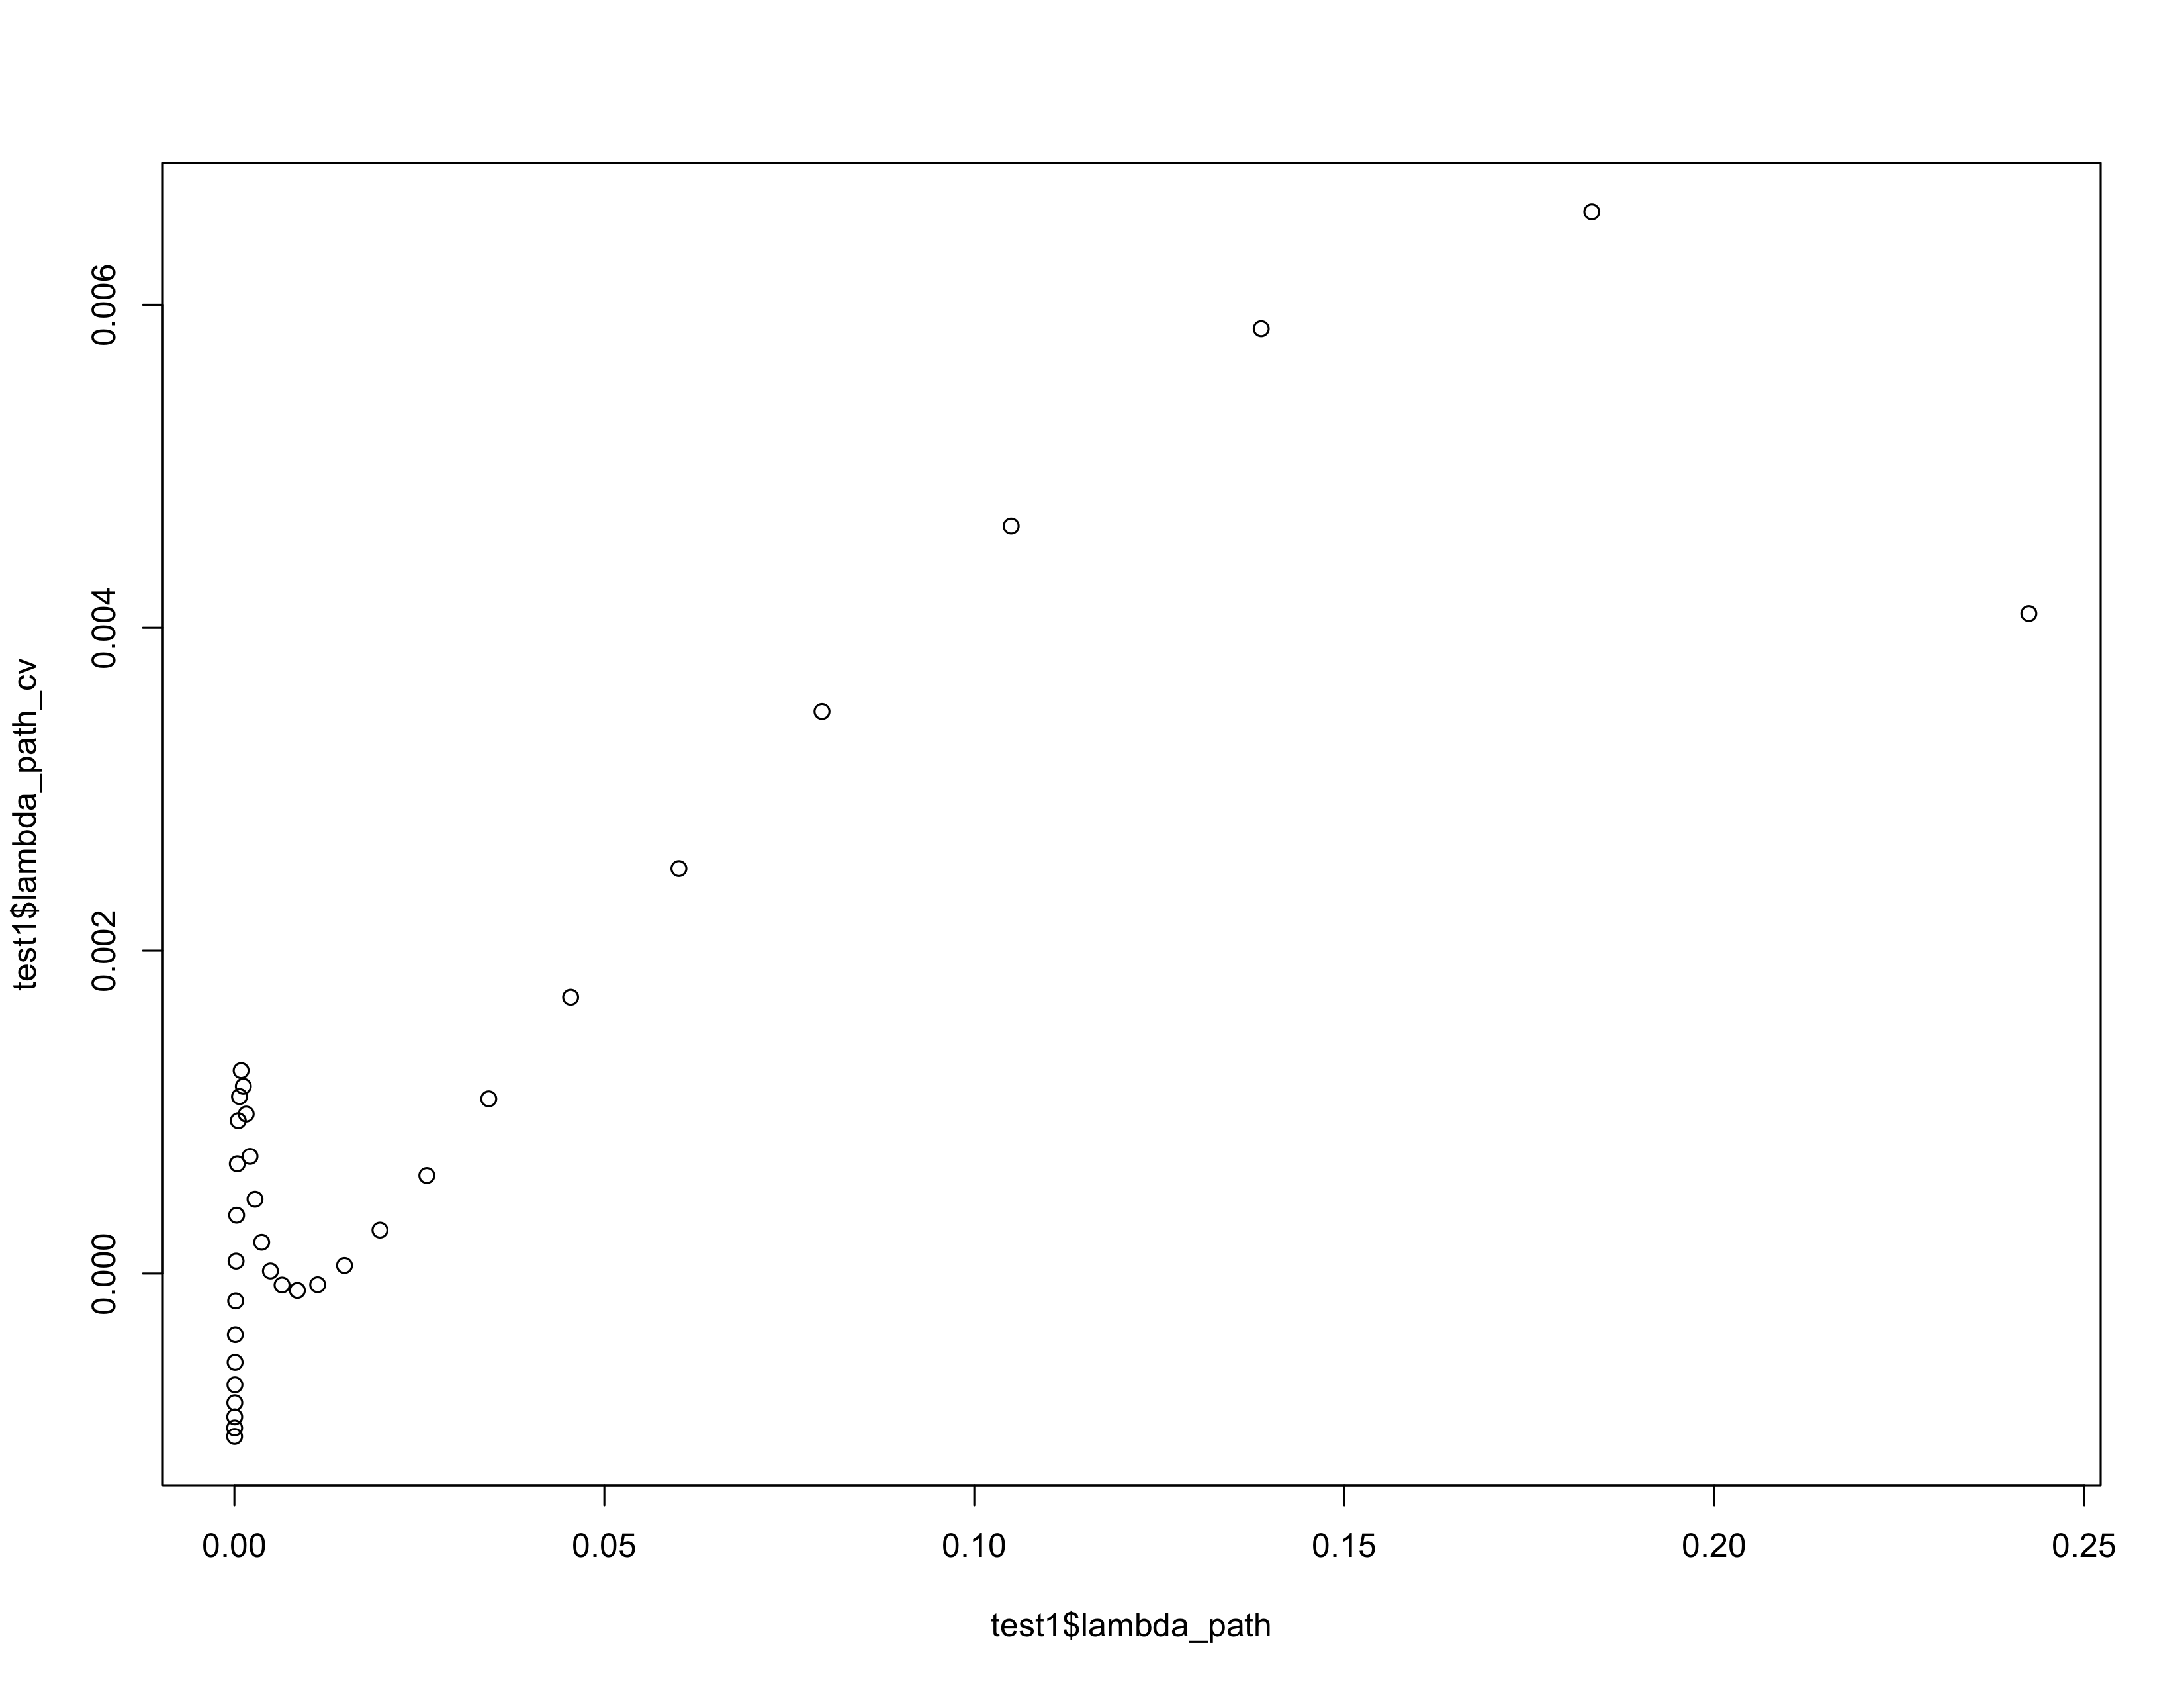
\includegraphics[width=1\linewidth]{./result_plot/fix_k/3wrong_path_plot}
\end{subfigure}%
\begin{subfigure}{.5\textwidth}
  \centering
  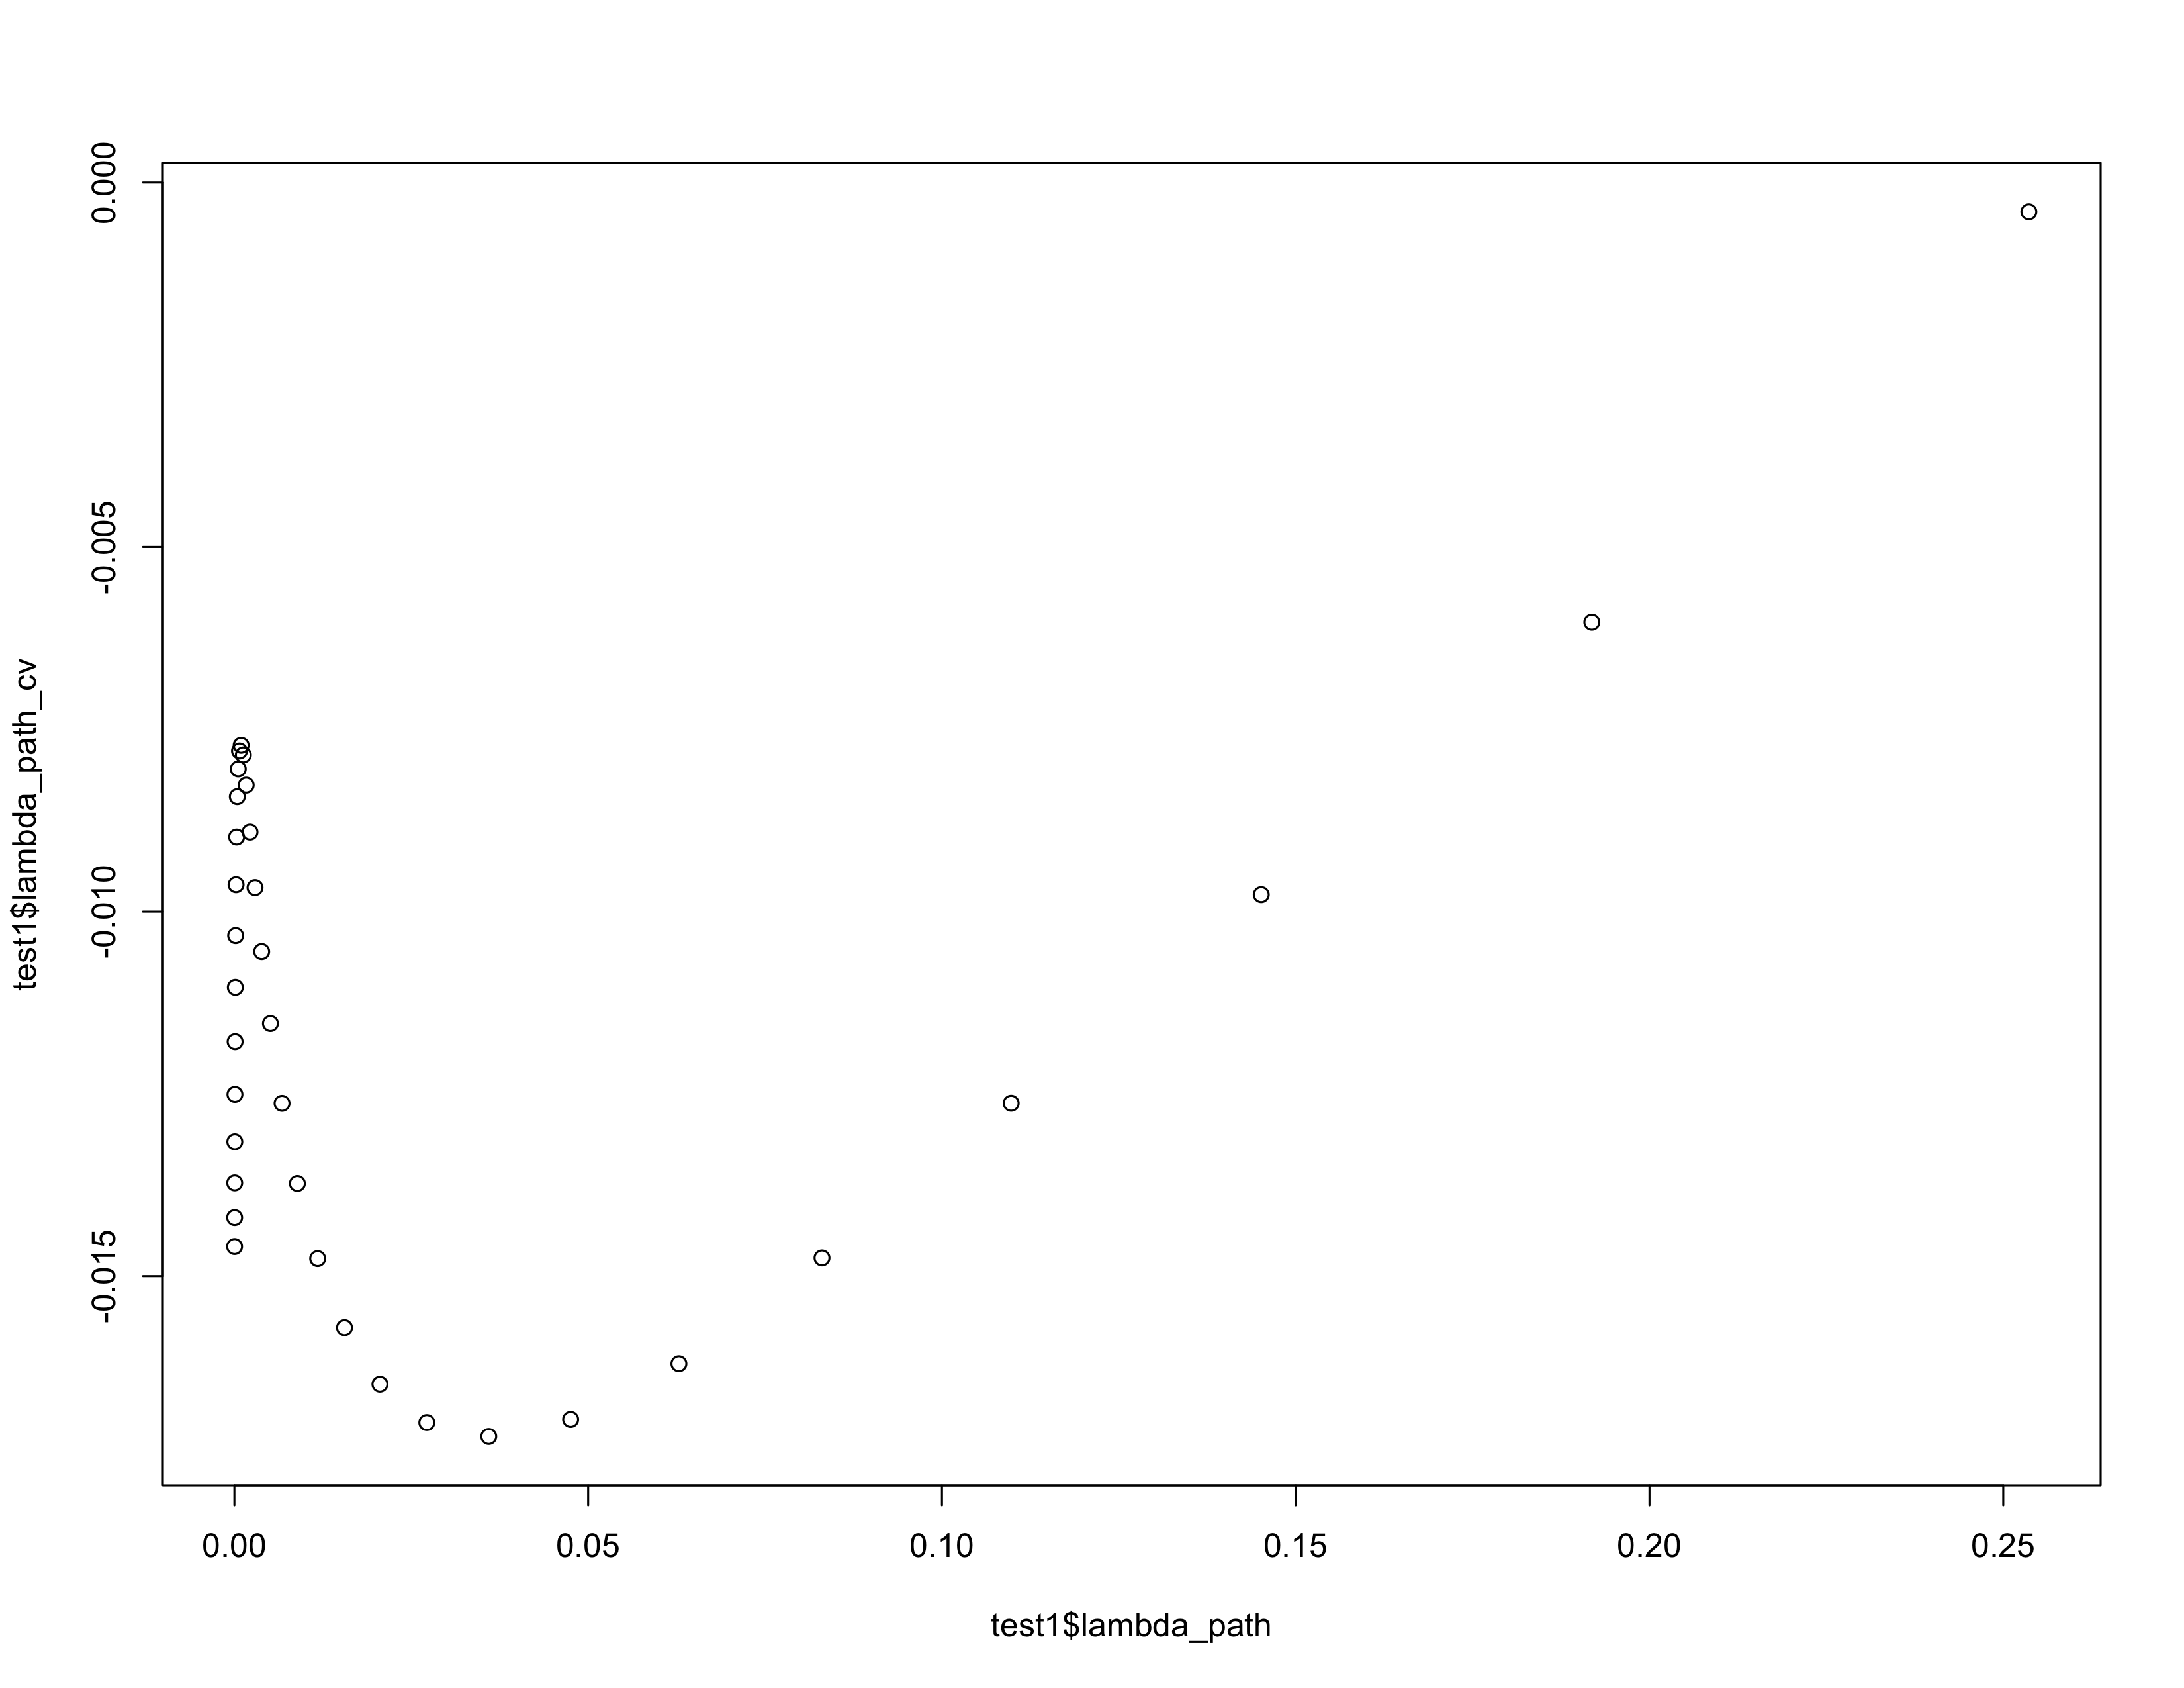
\includegraphics[width=1\linewidth]{./result_plot/fix_k/4wrong_path_plot}
\end{subfigure}

\end{figure}

\begin{figure}[H]
\centering
\begin{subfigure}{0.5\textwidth}
  \centering
  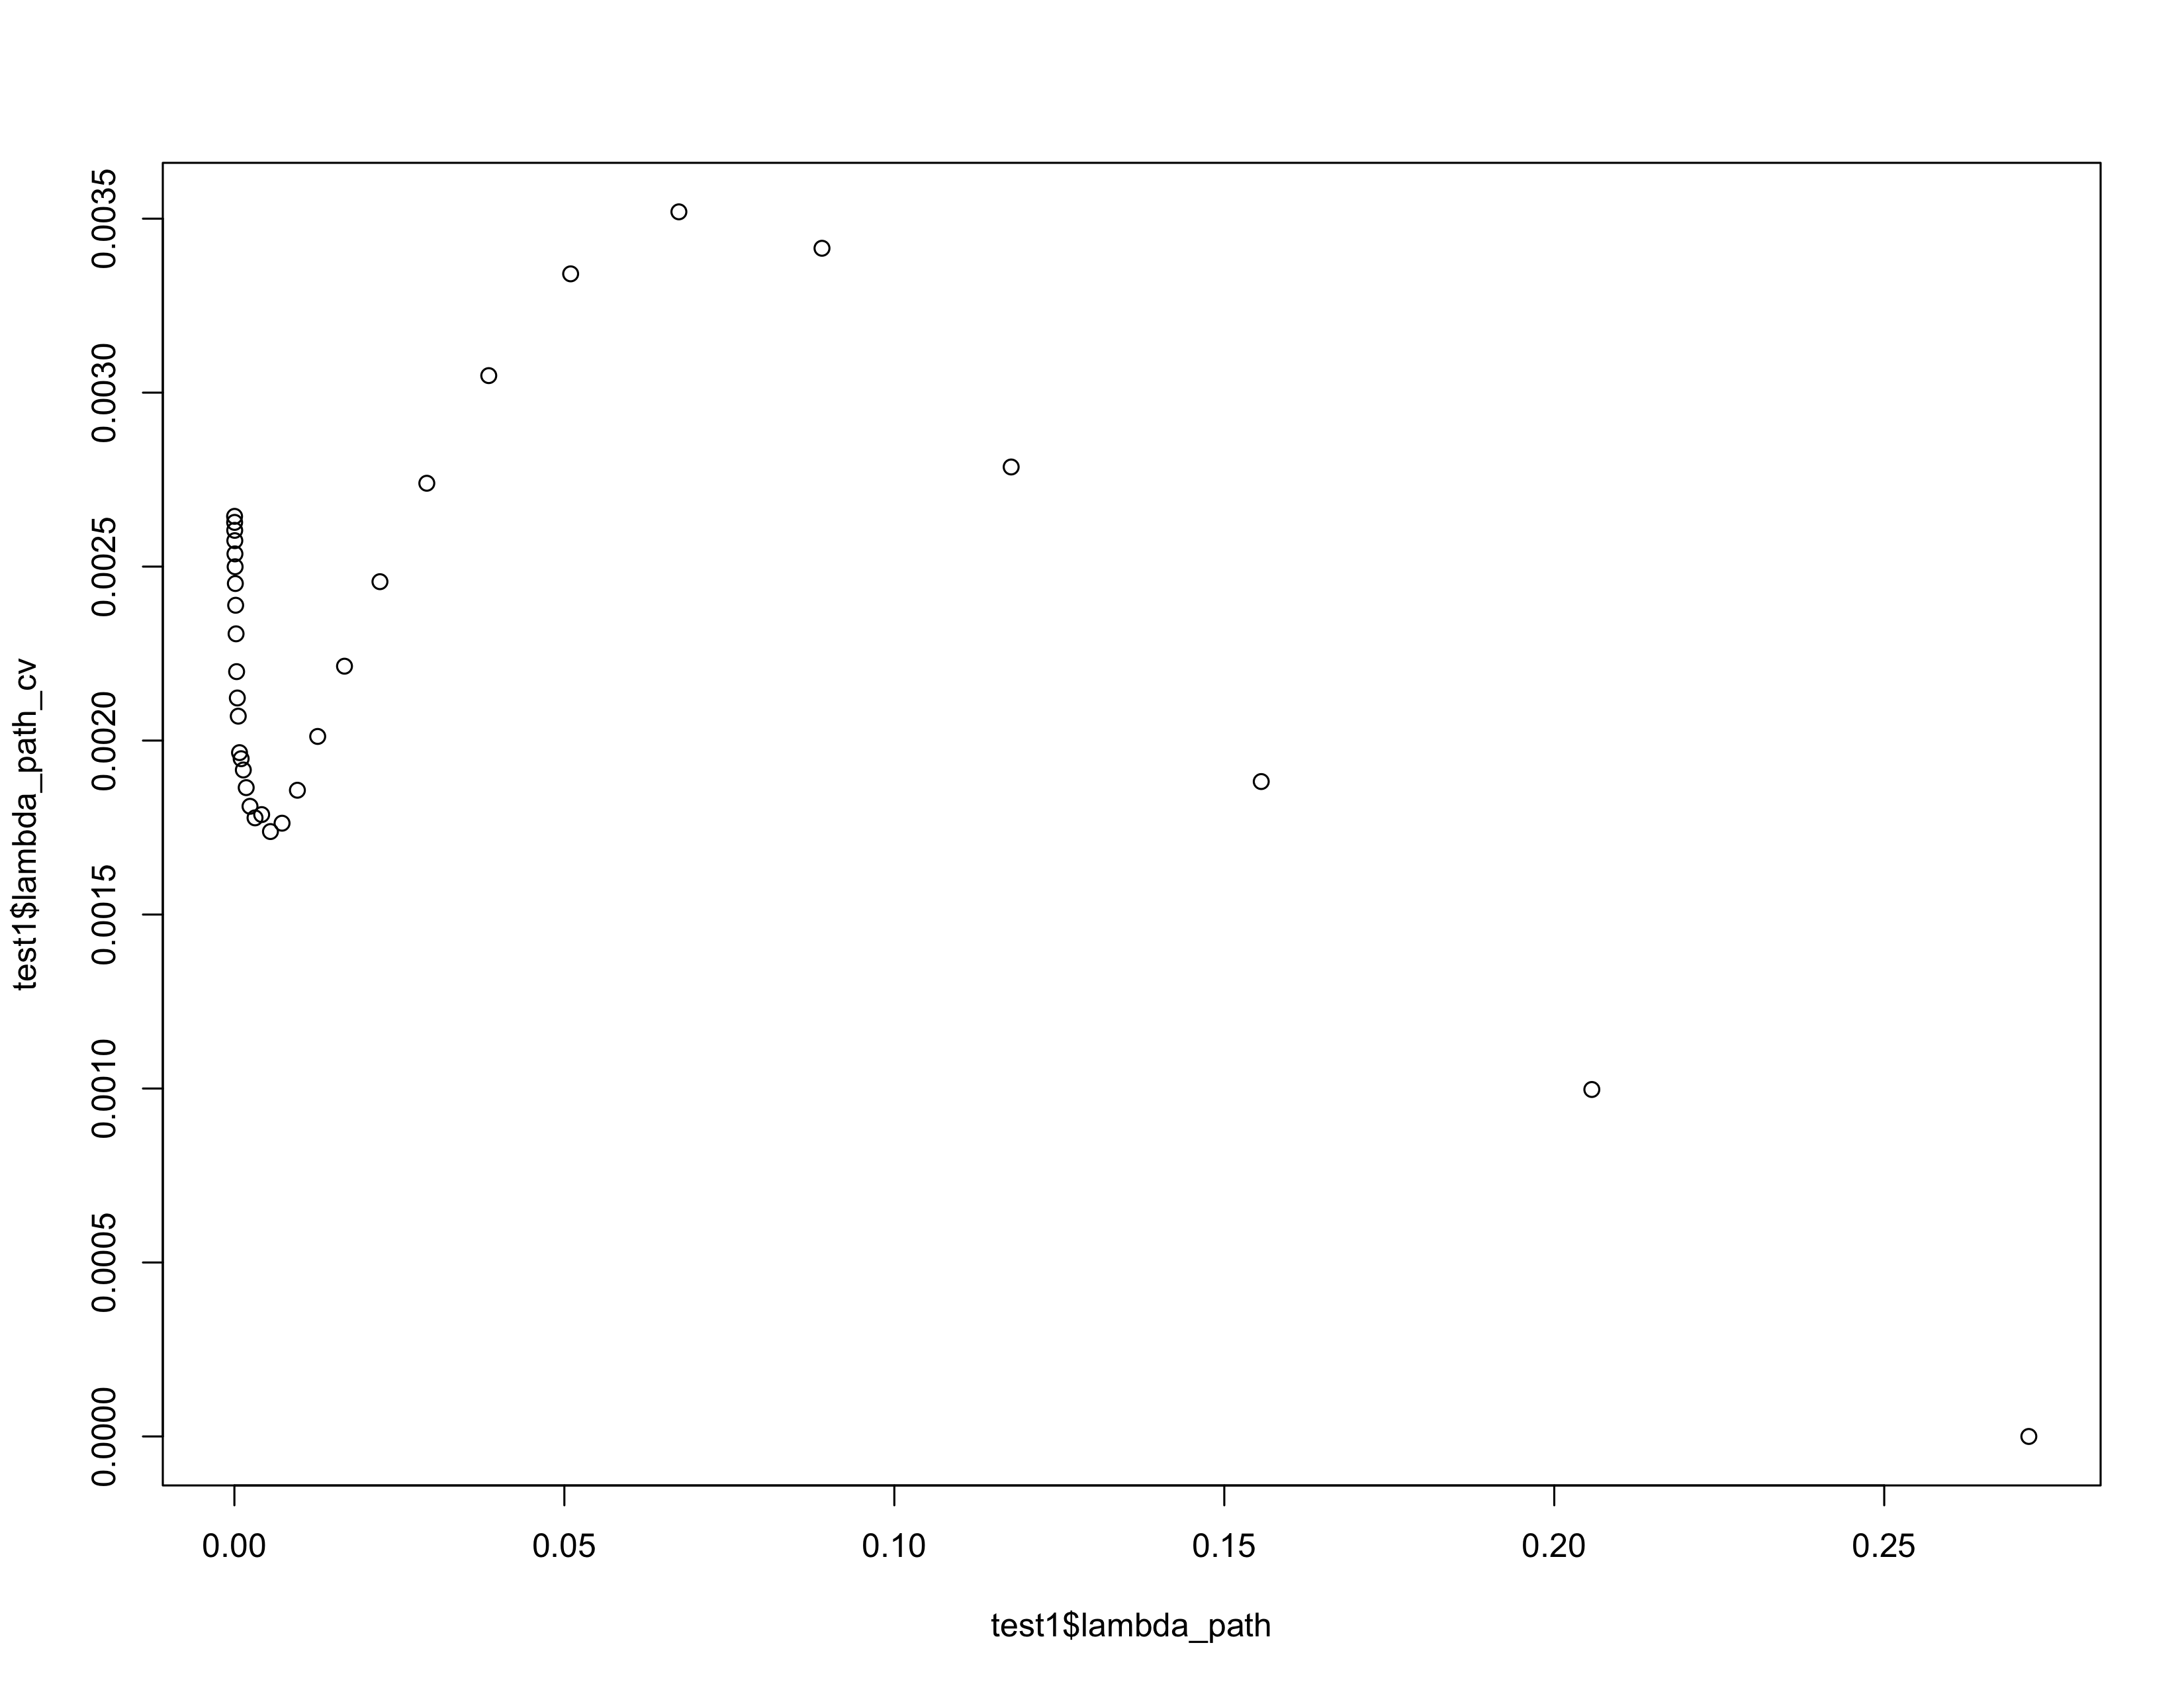
\includegraphics[width=1\linewidth]{./result_plot/fix_k/5wrong_path_plot}
\end{subfigure}%
\begin{subfigure}{.5\textwidth}
  \centering
  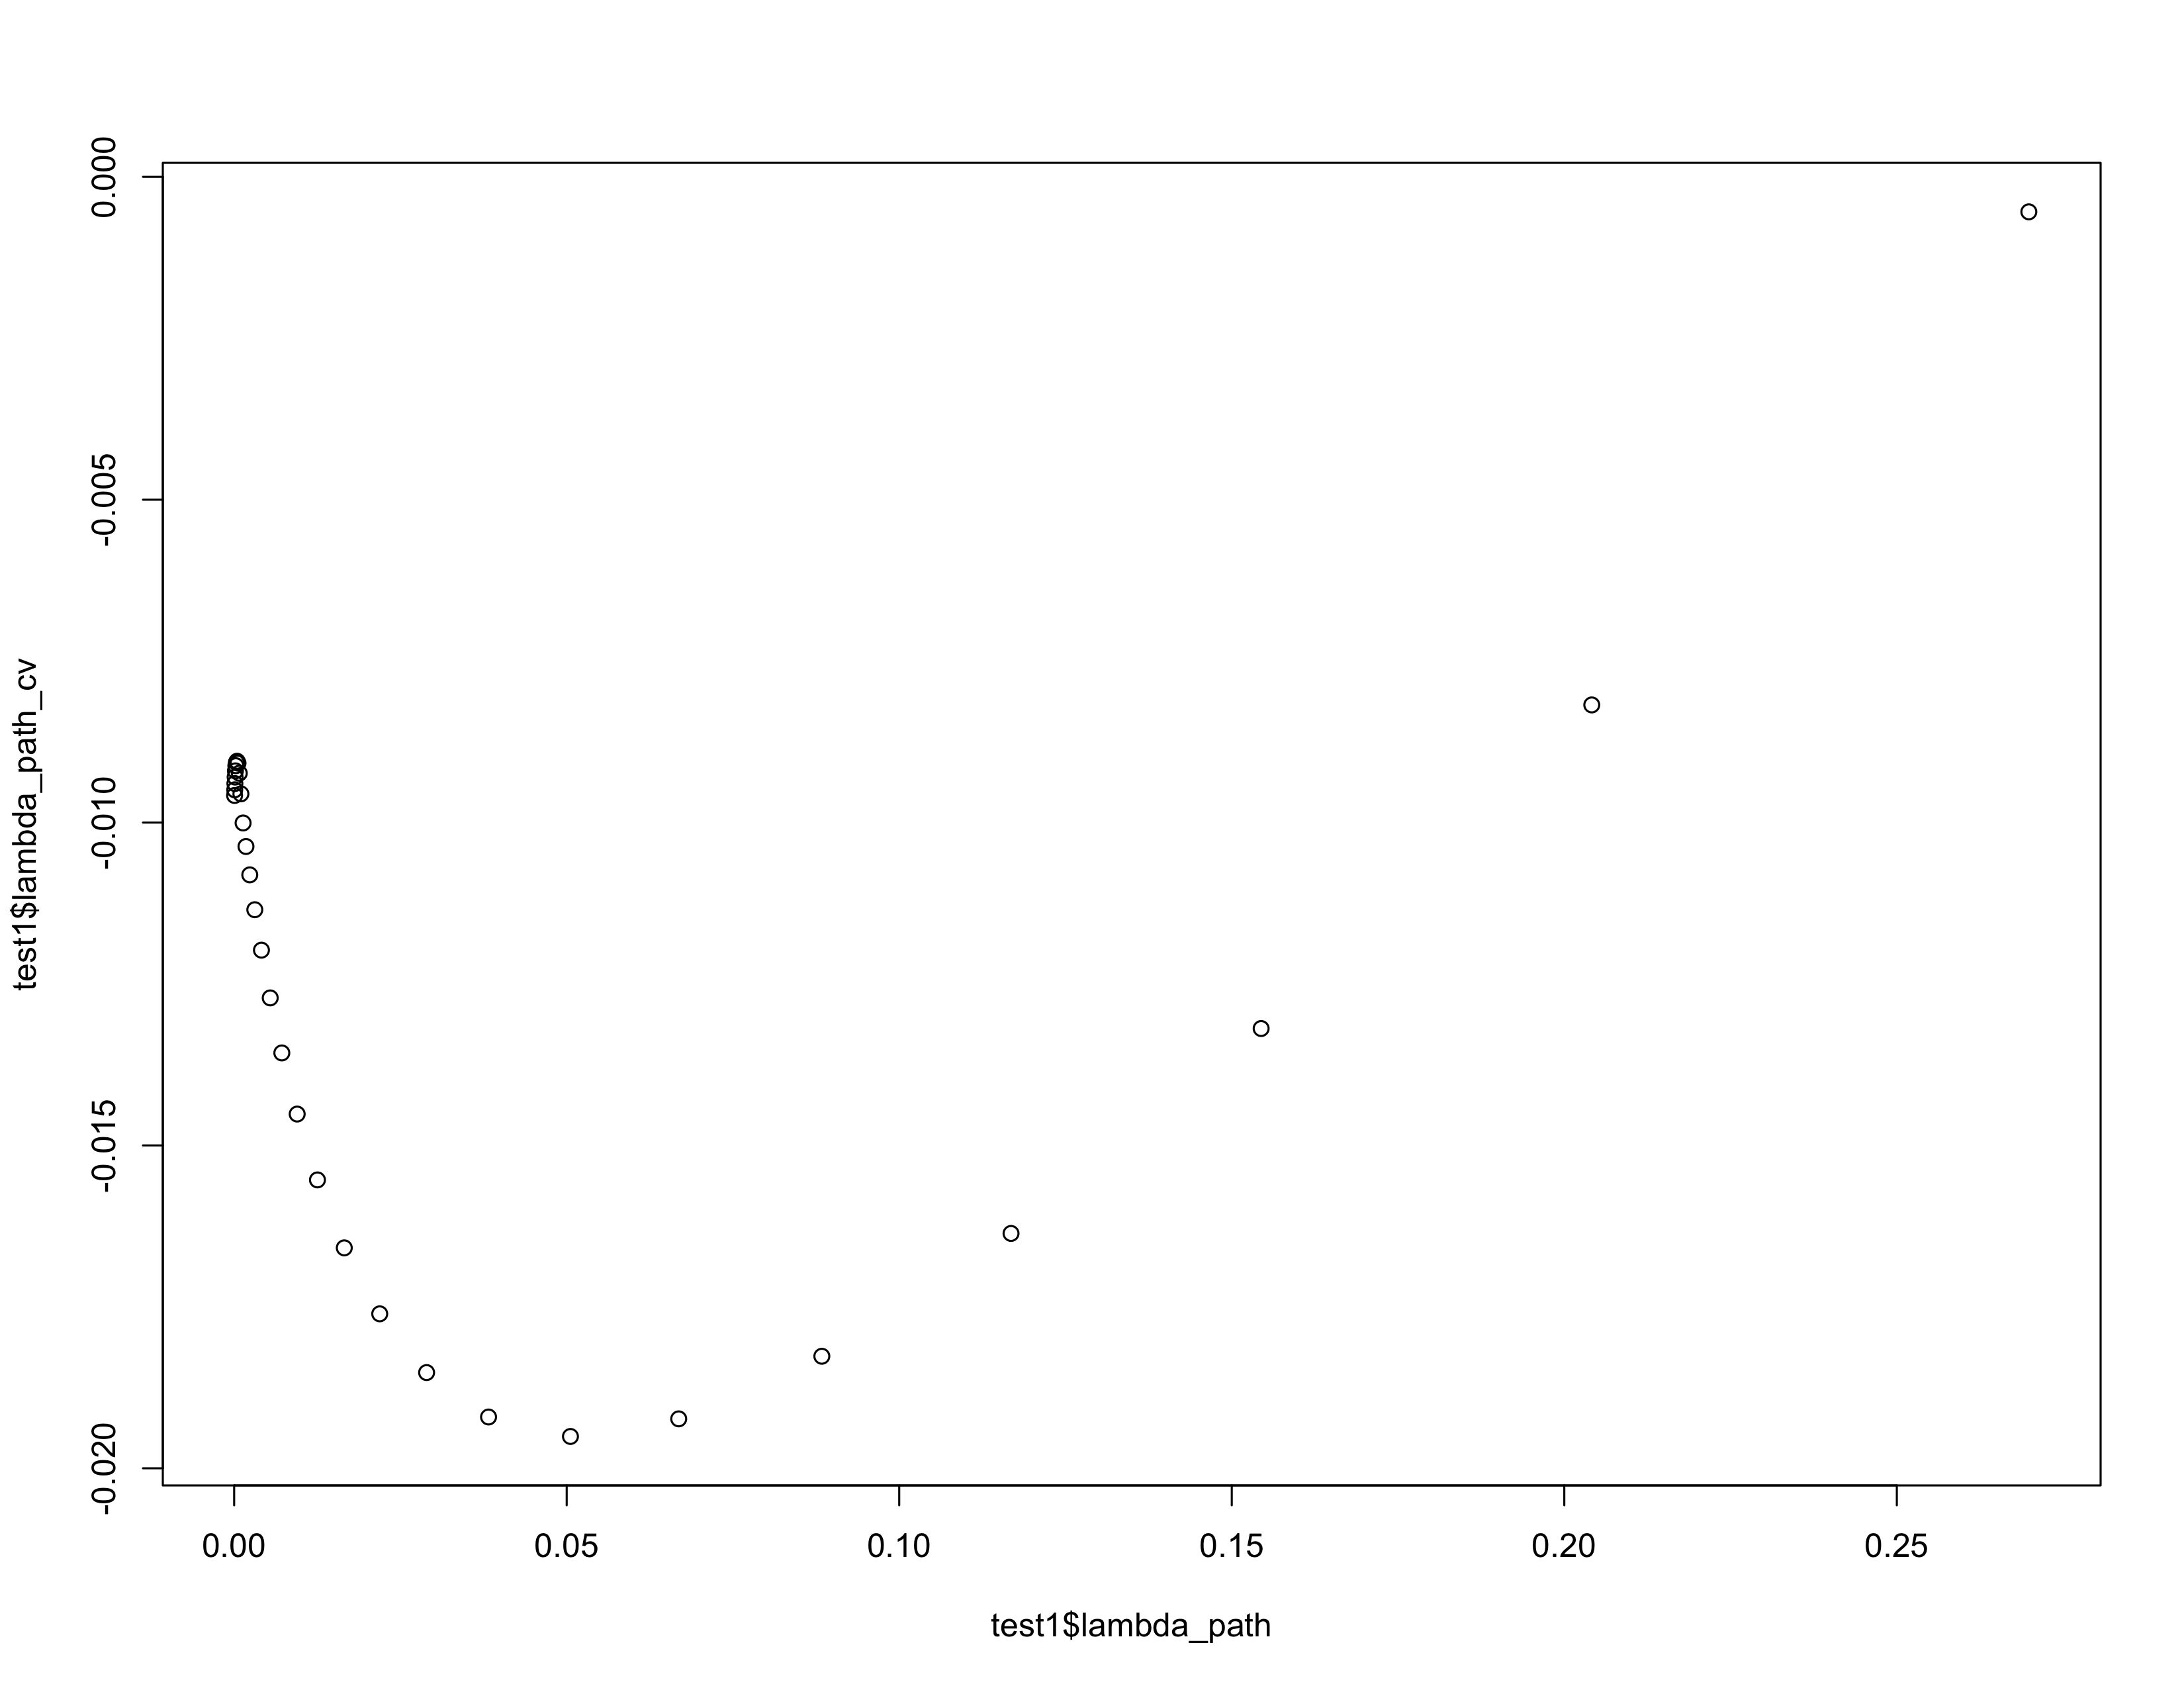
\includegraphics[width=1\linewidth]{./result_plot/fix_k/6wrong_path_plot}
\end{subfigure}

\end{figure}

\begin{figure}[H]
\centering
\begin{subfigure}{0.5\textwidth}
  \centering
  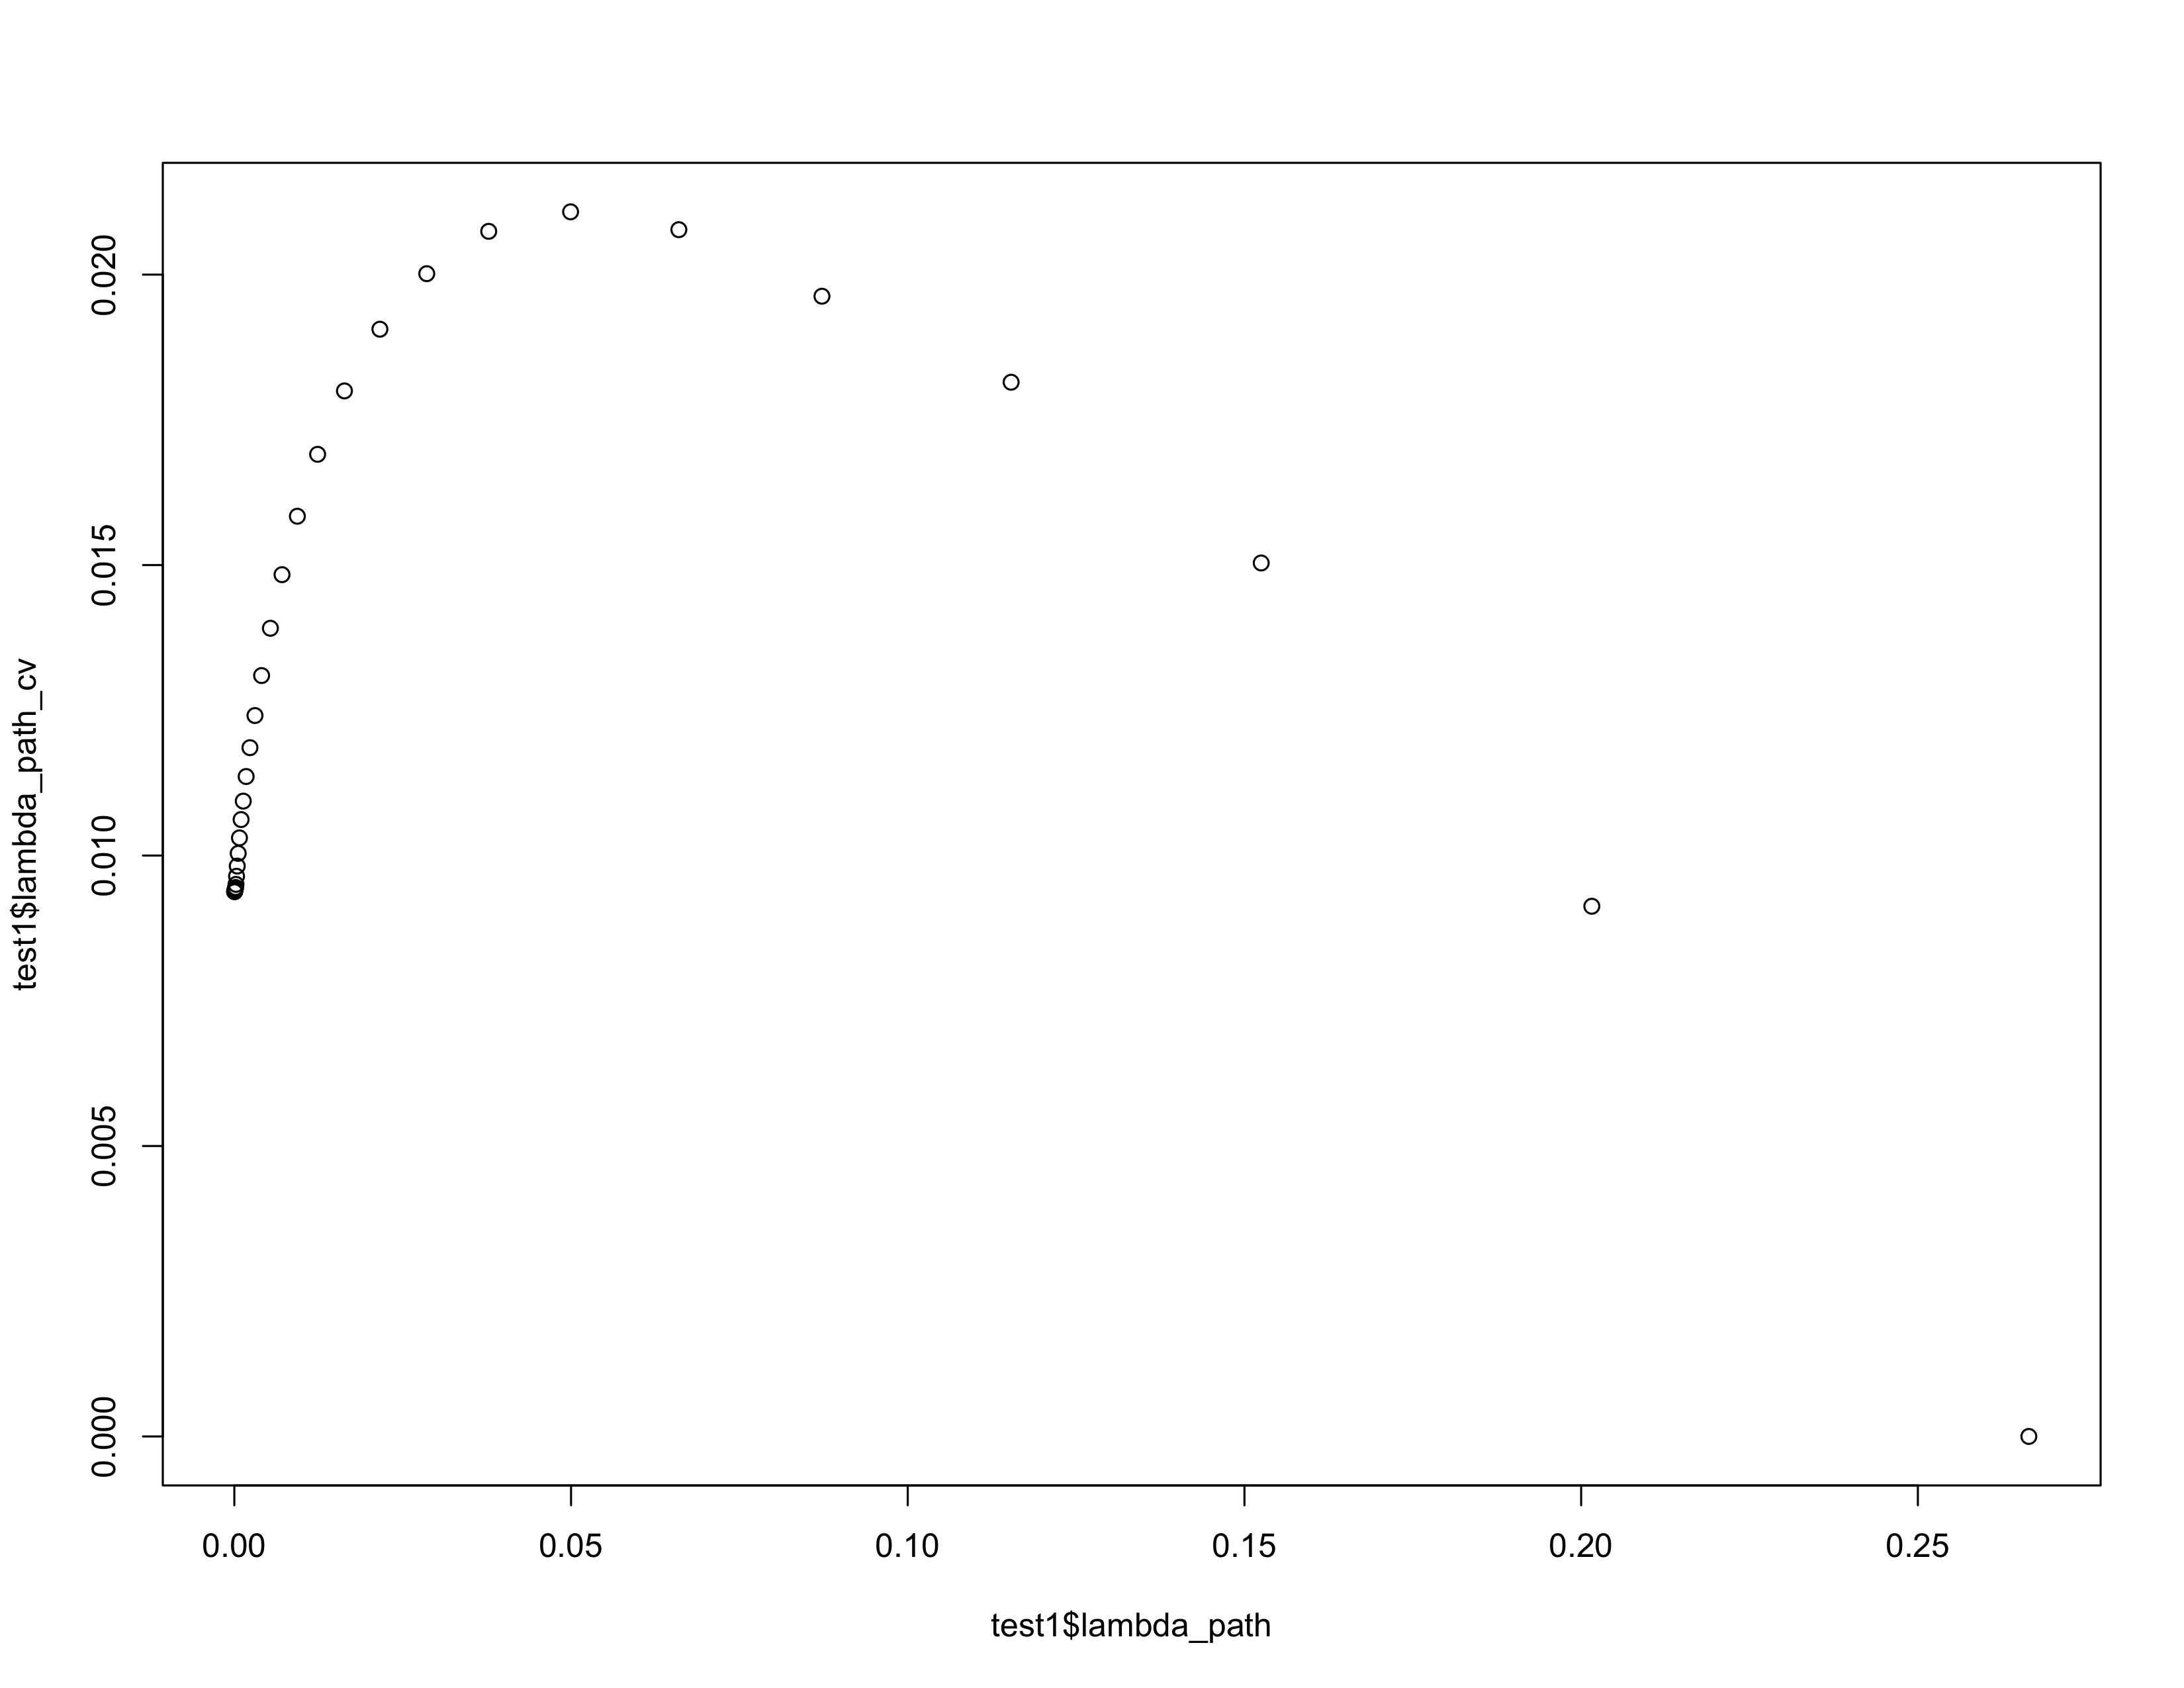
\includegraphics[width=1\linewidth]{./result_plot/fix_k/7wrong_path_plot}
\end{subfigure}%
\begin{subfigure}{.5\textwidth}
  \centering
  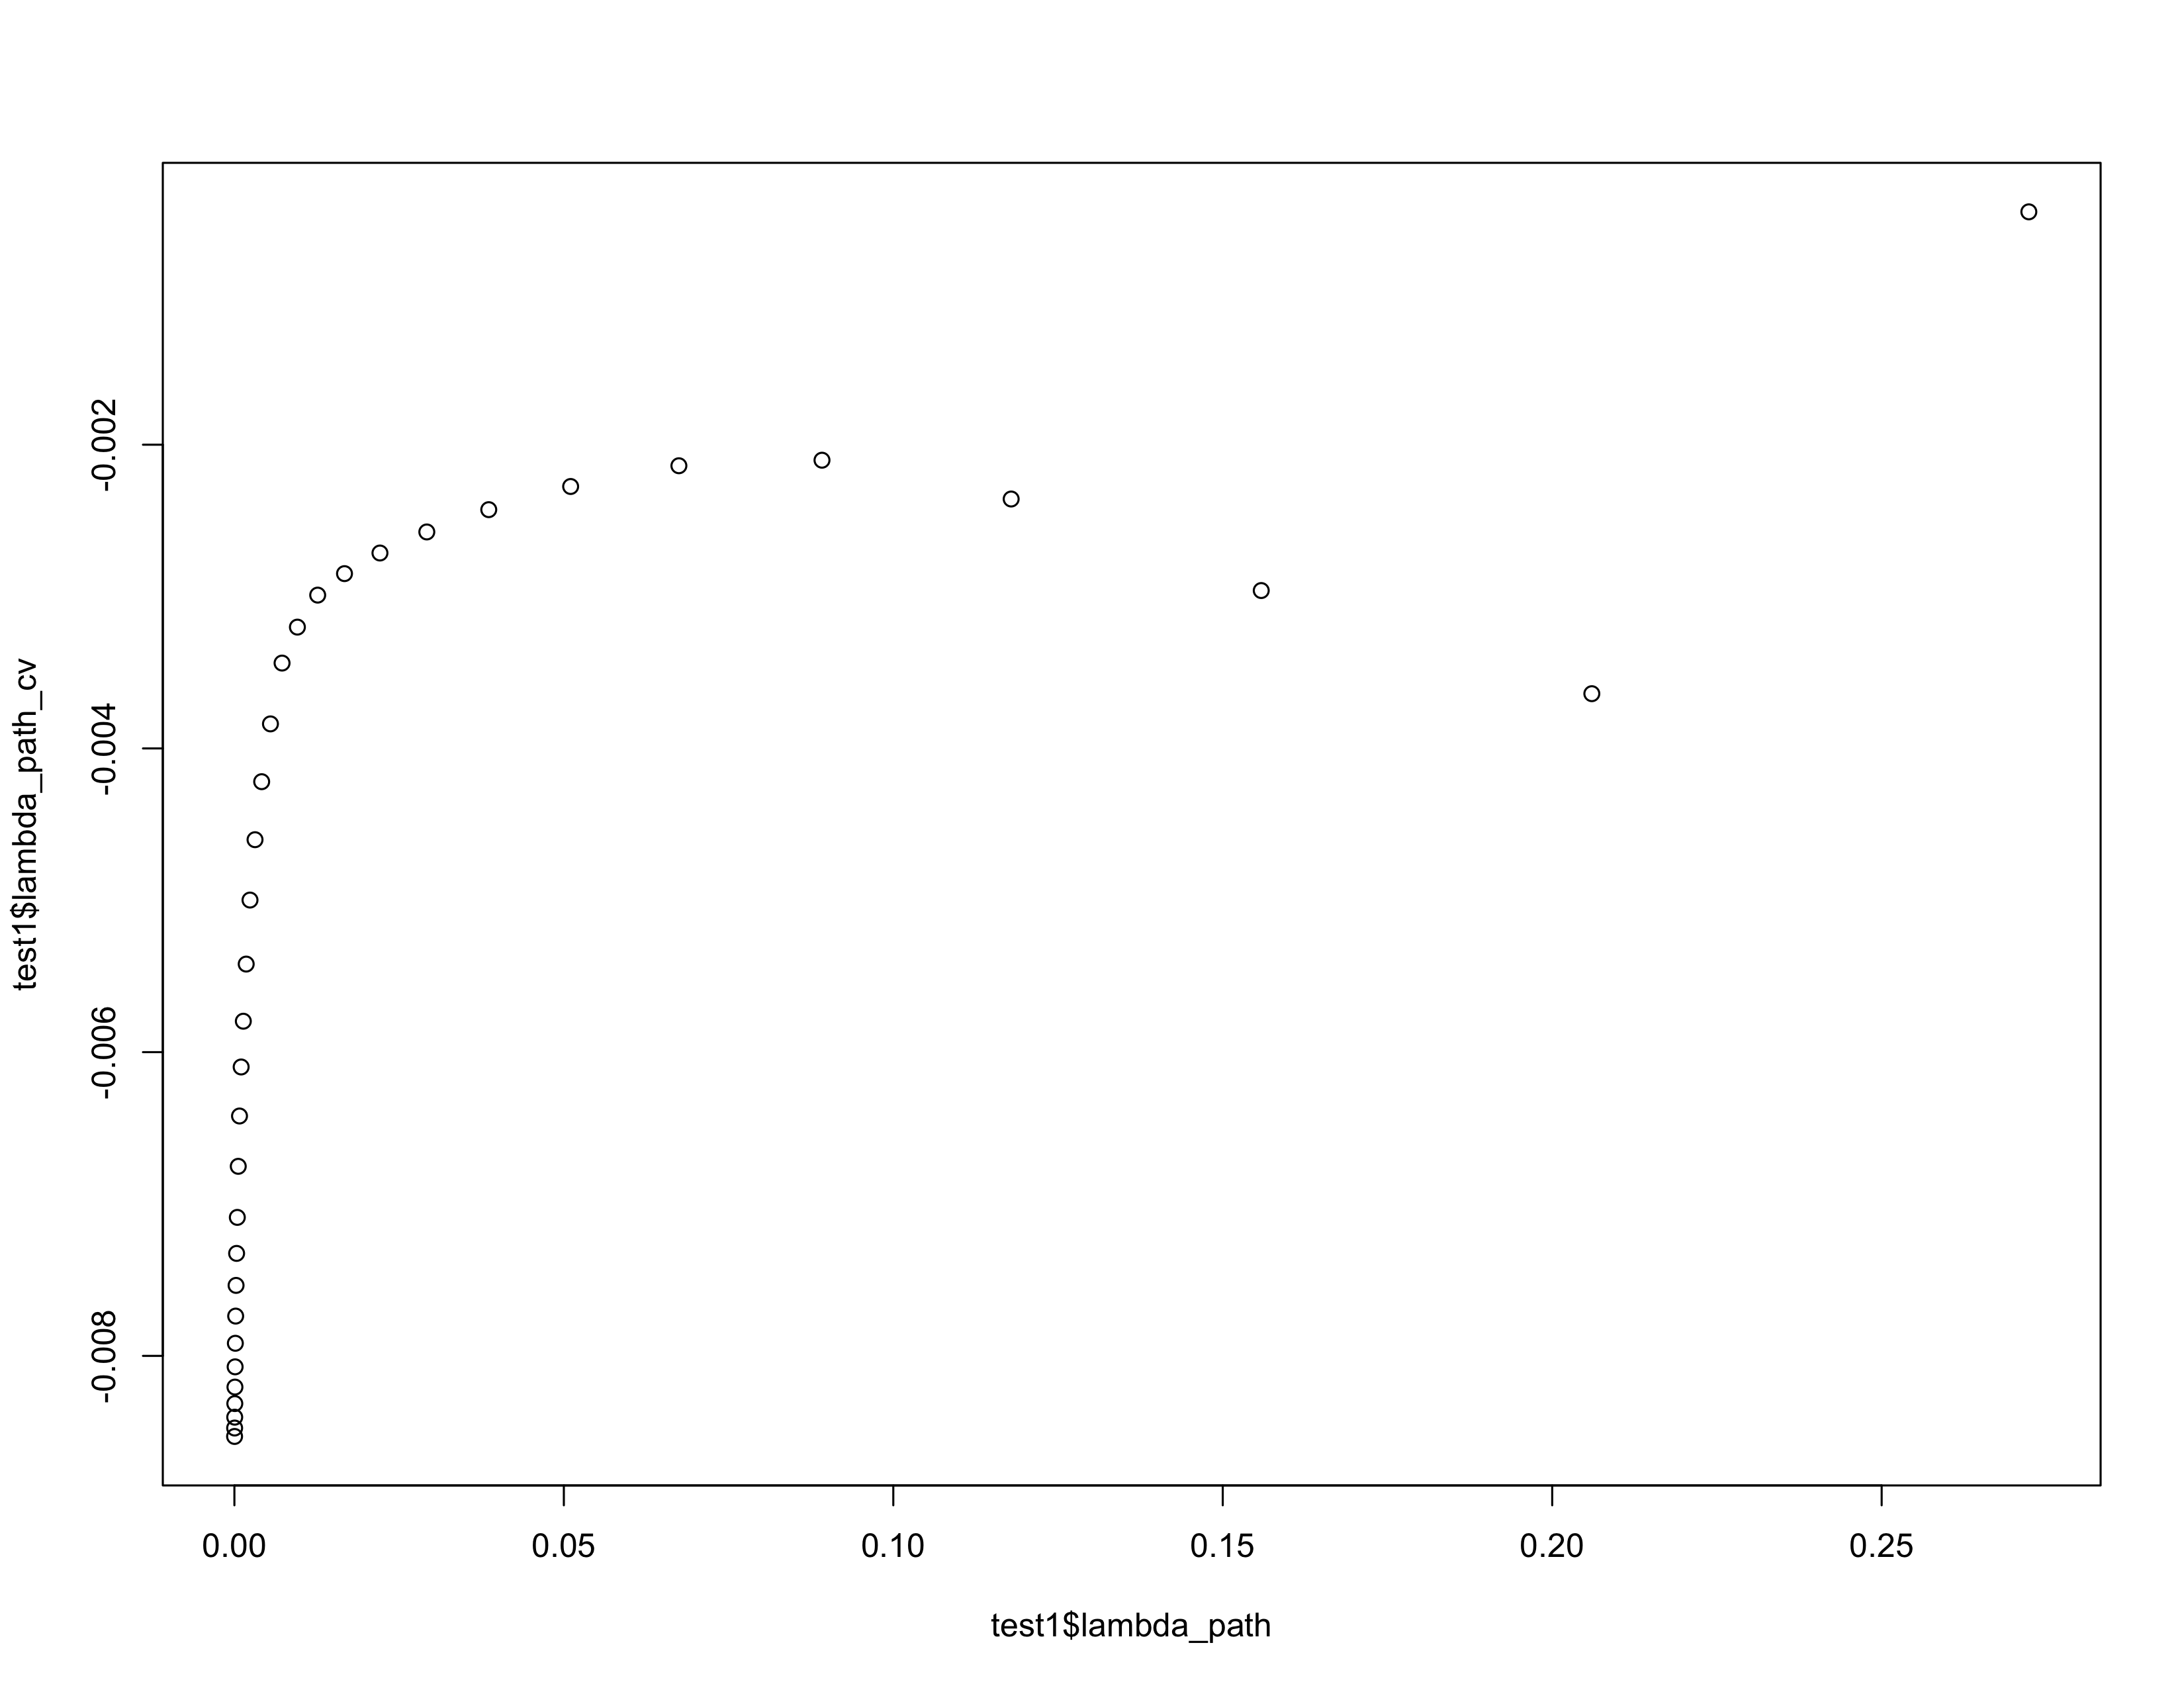
\includegraphics[width=1\linewidth]{./result_plot/fix_k/8wrong_path_plot}
\end{subfigure}

\end{figure}

\begin{figure}[H]
\centering
\begin{subfigure}{0.5\textwidth}
  \centering
  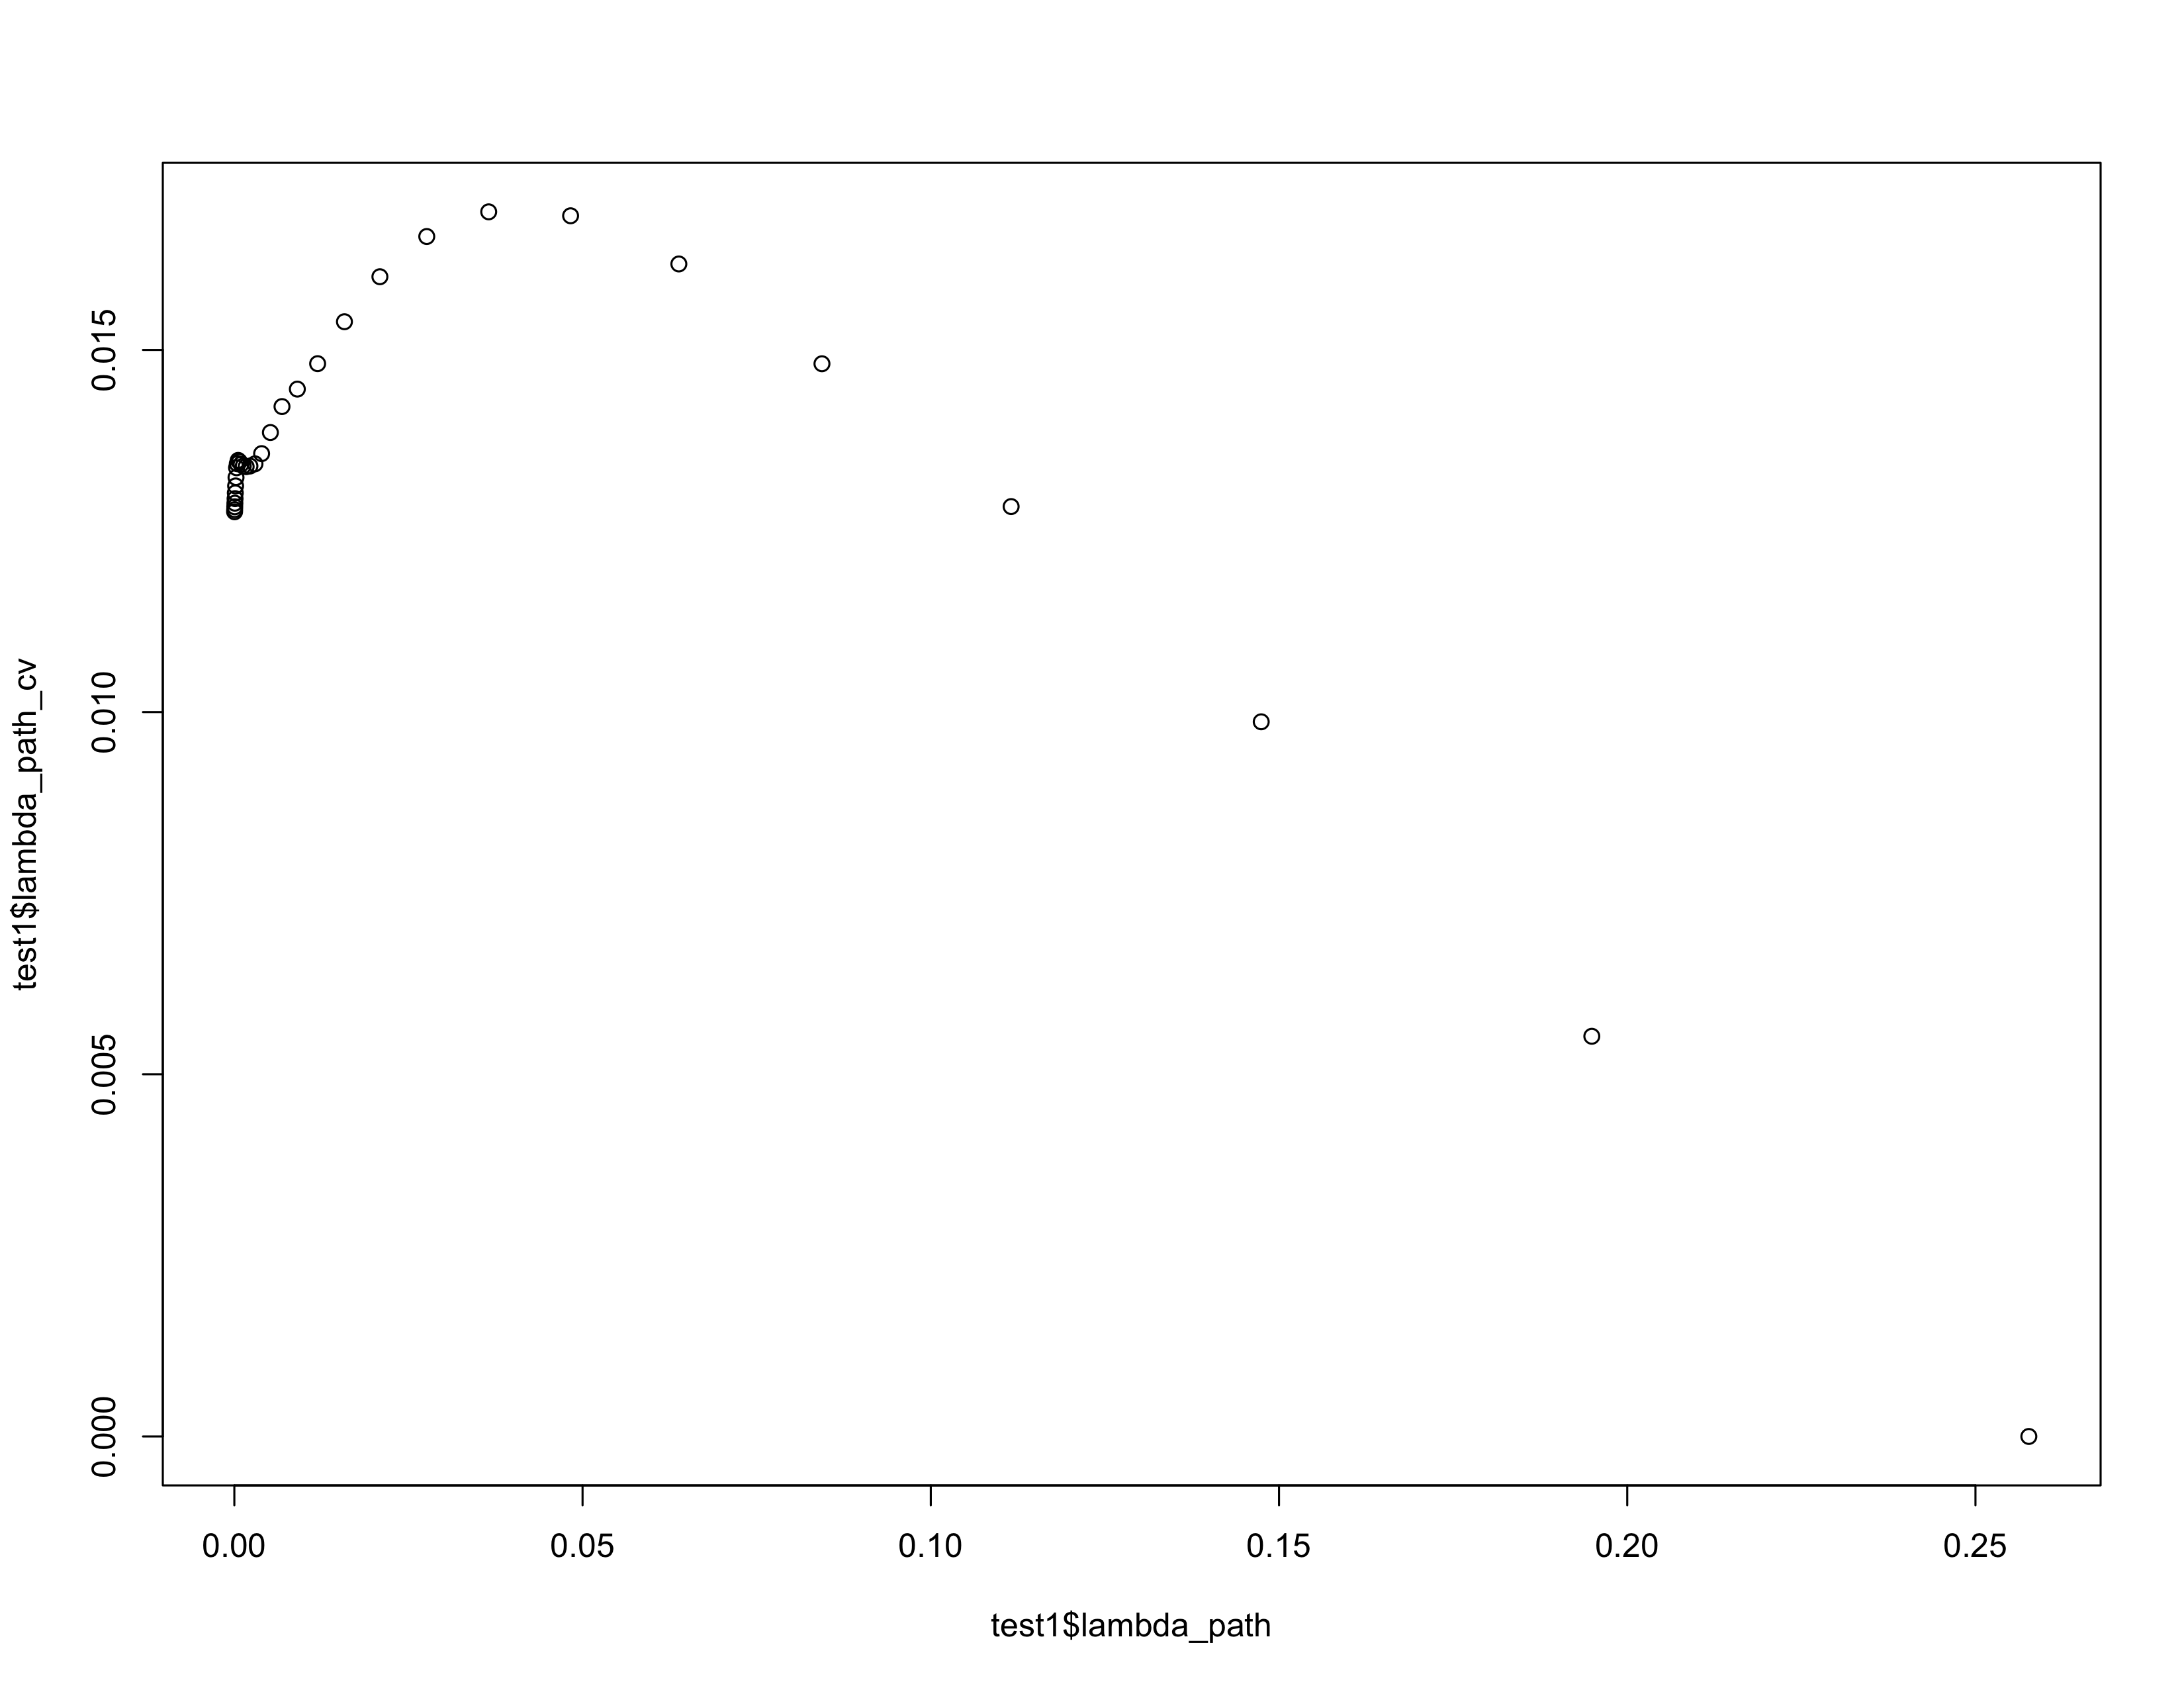
\includegraphics[width=1\linewidth]{./result_plot/fix_k/9wrong_path_plot}
\end{subfigure}%
\begin{subfigure}{.5\textwidth}
  \centering
  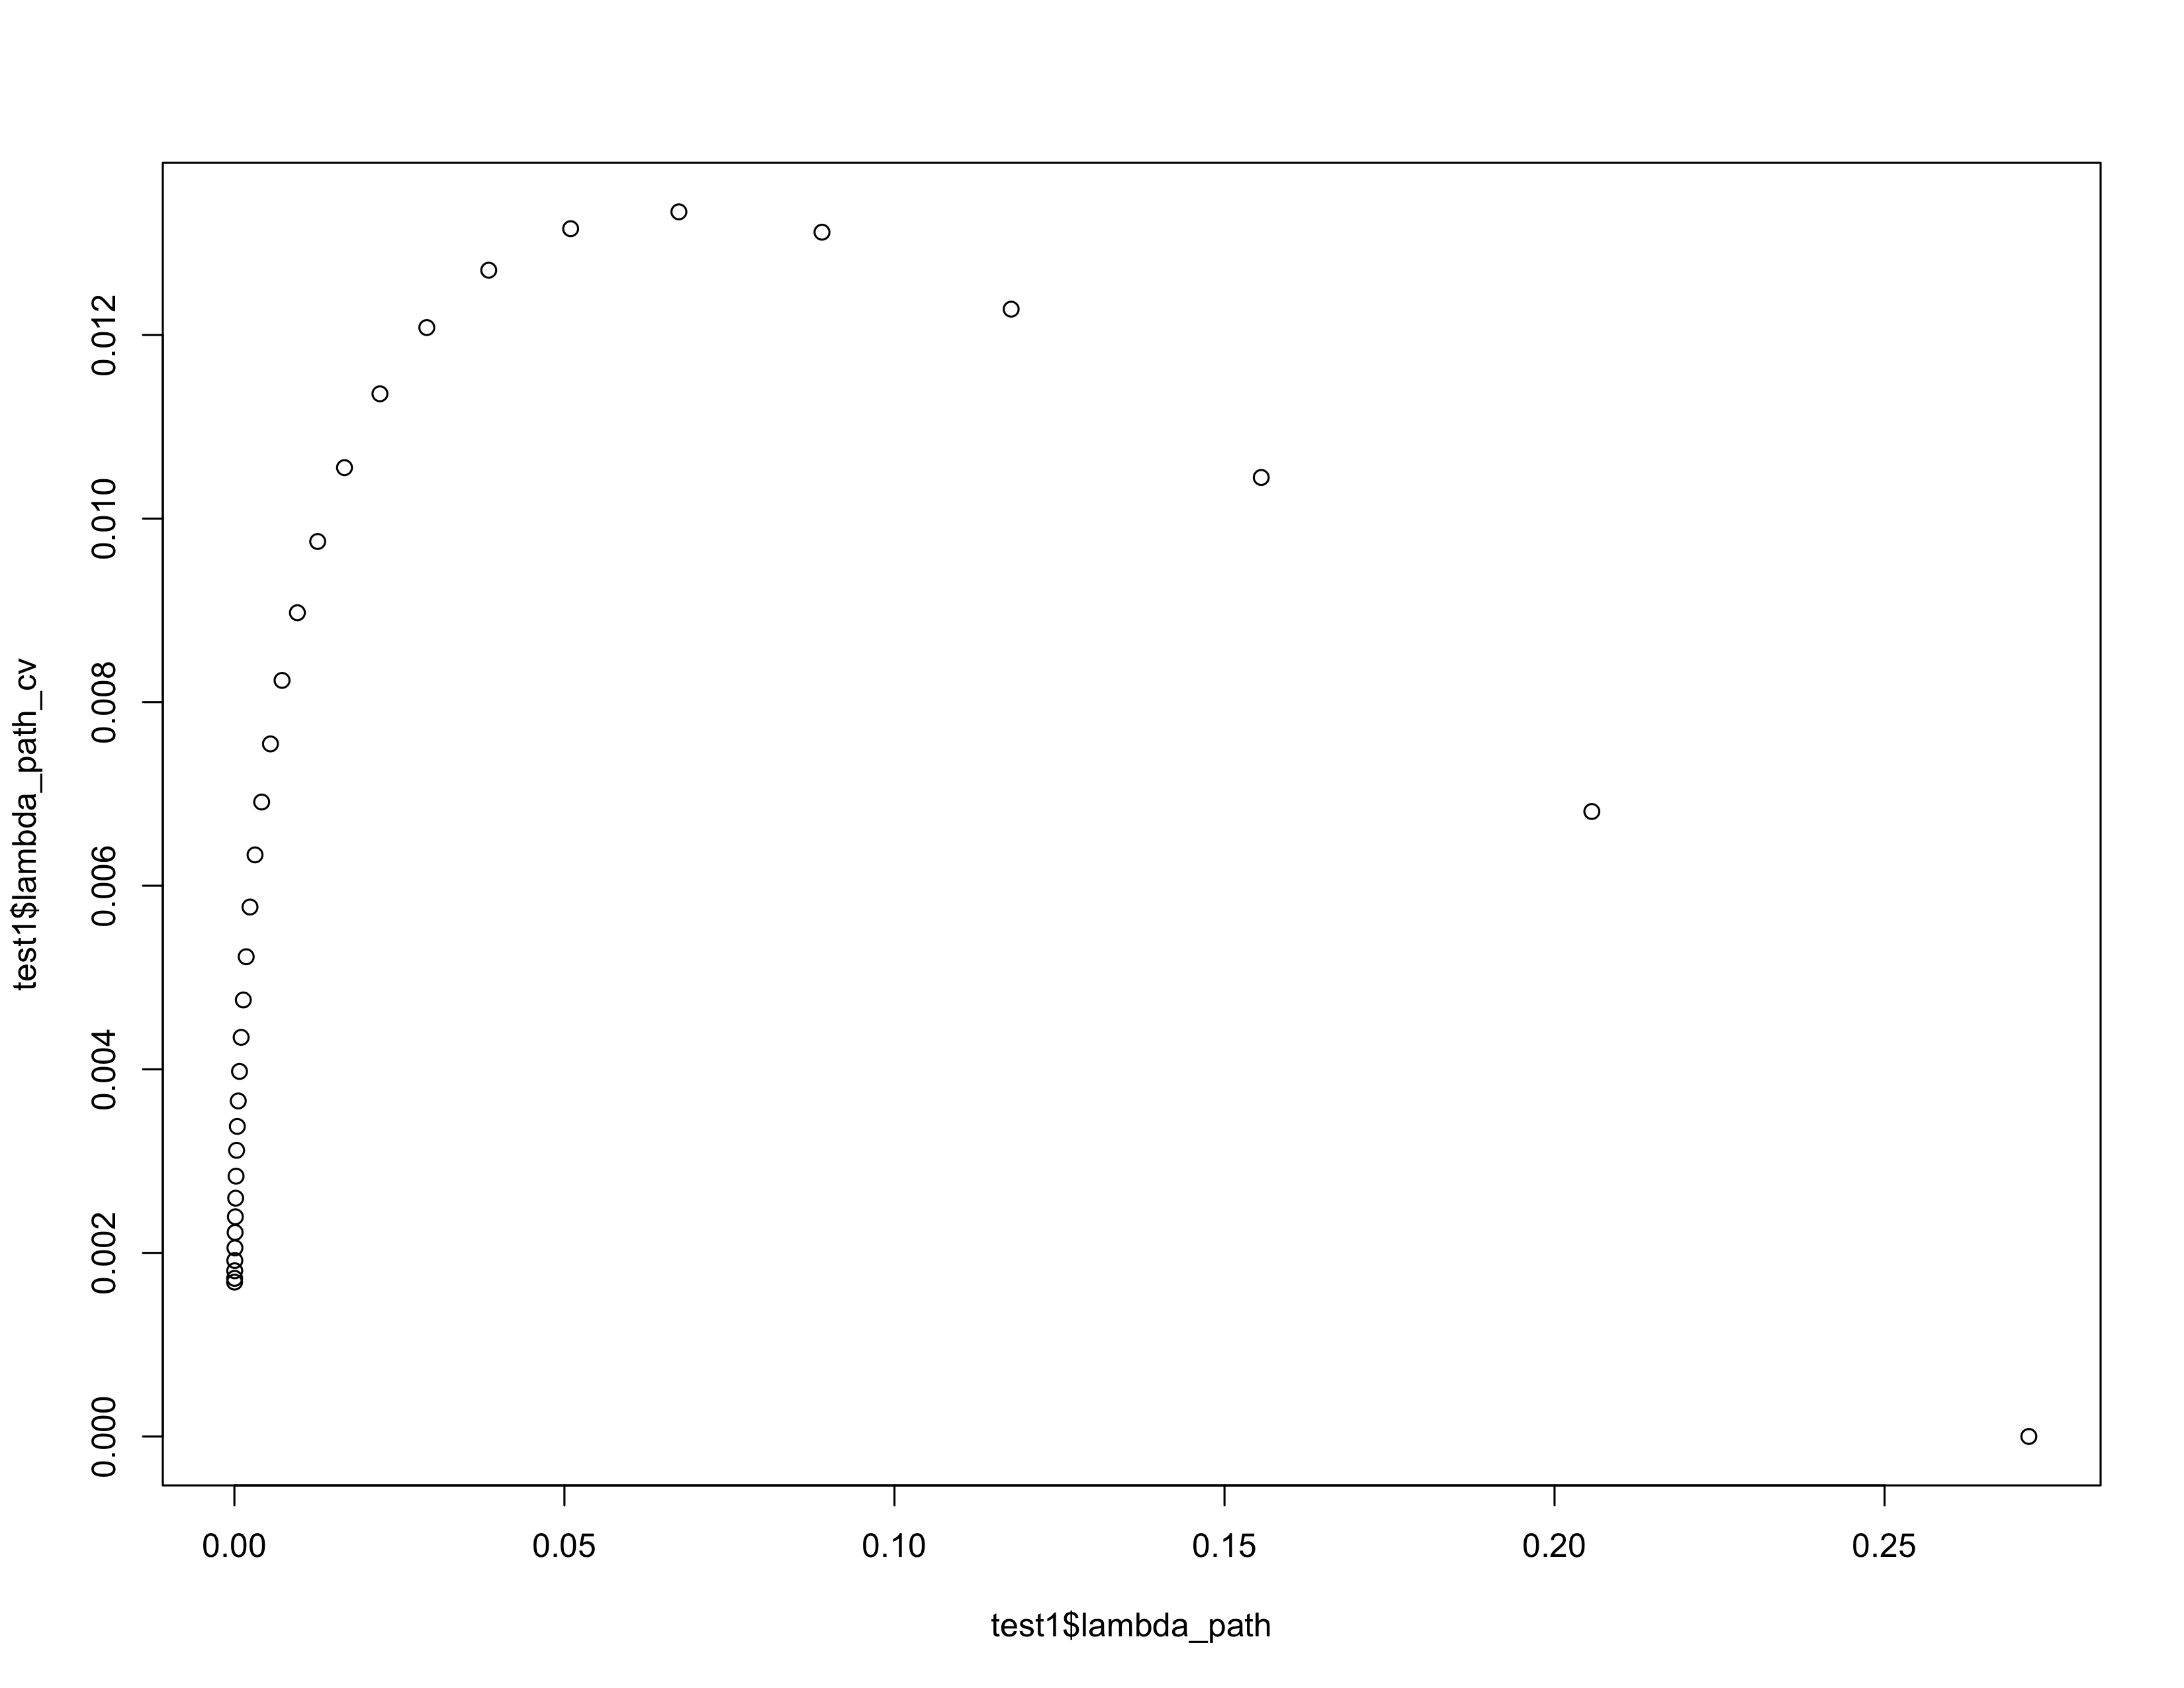
\includegraphics[width=1\linewidth]{./result_plot/fix_k/10wrong_path_plot}
\end{subfigure}

\end{figure}


\section{use only one part of k dataset in the first term}
\label{sec:k}
In this part, I used only the $\text{k}^{\text{th}}$ part in our dataset for first term in the summation, and used anther k-1 dataset to generate the $\hat{\beta}$  
In this section, we define:
$$
\argmin_{\lambda}\text{cv}(\lambda)=\argmin_{\lambda}\sum_{k=1}^5\{l^{(k)}(\hat{\beta}_\lambda^{(-k)})-l^{(-k)}\hat{\beta}_(\lambda^{(-k)})\}^2
$$
The plots we got are

\begin{figure}[H]
\centering
\begin{subfigure}{0.5\textwidth}
  \centering
  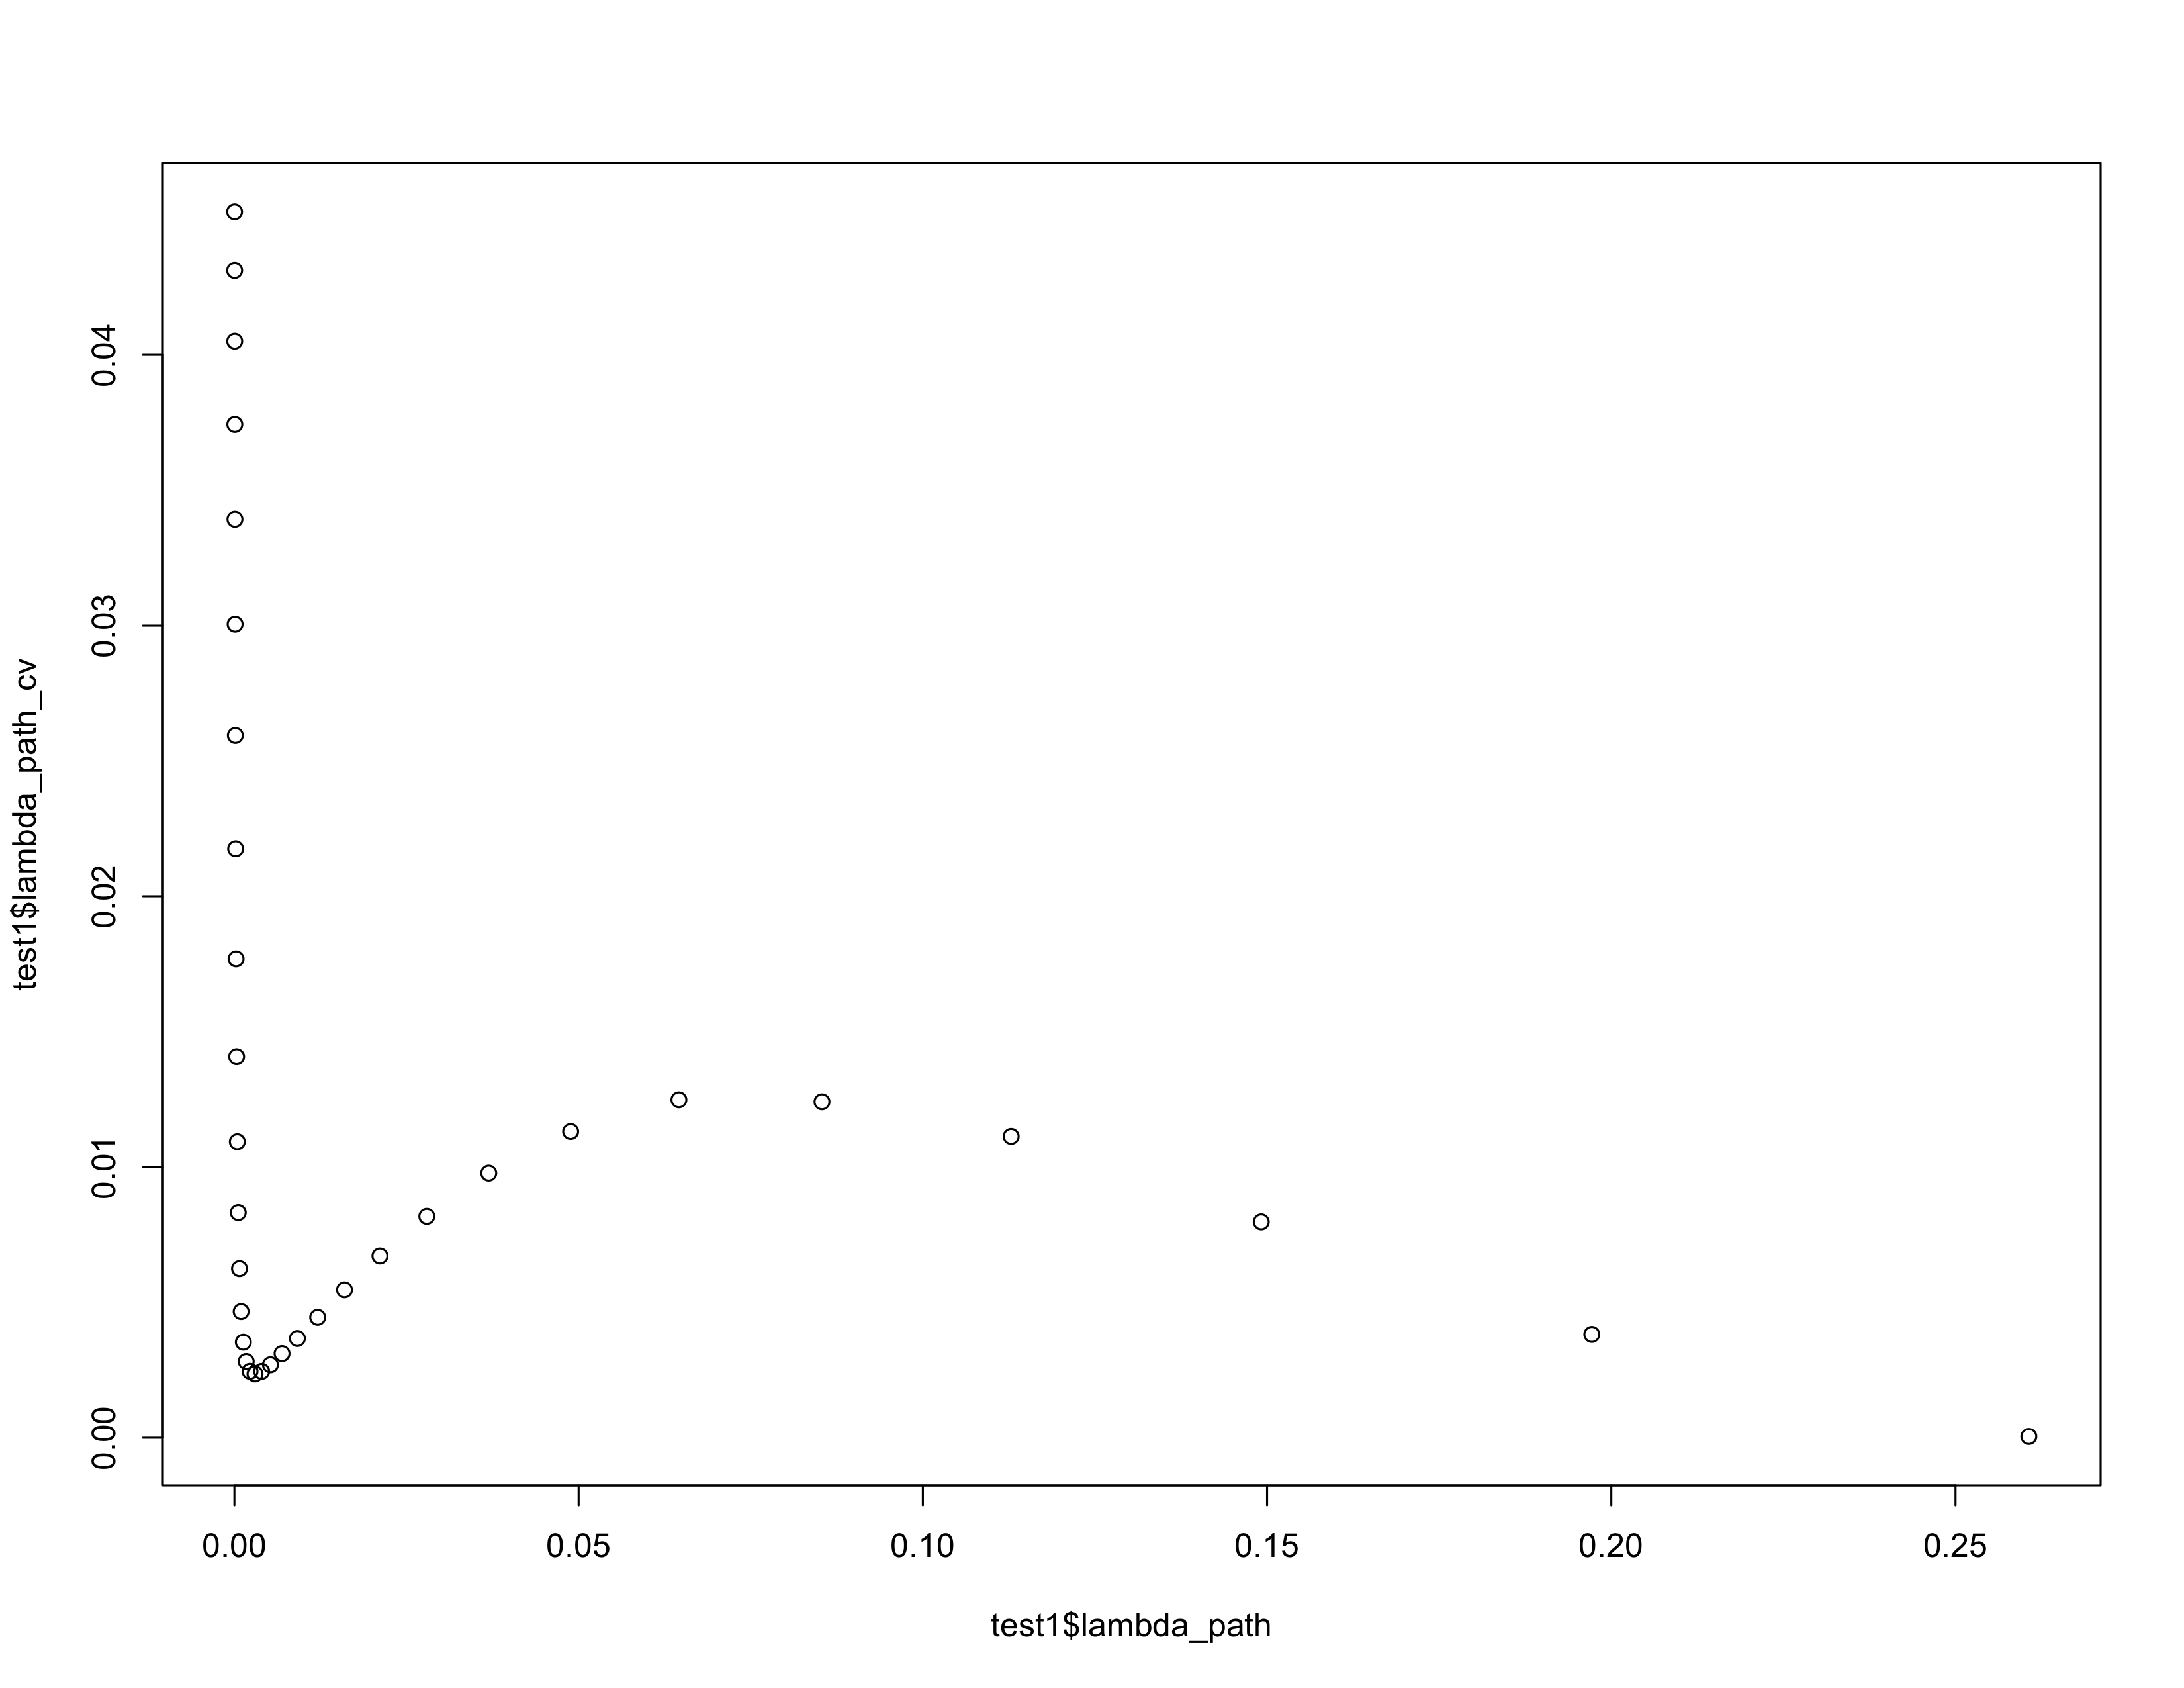
\includegraphics[width=1\linewidth]{./result_plot/ll_use_k/1wrong_path_plot}
\end{subfigure}%
\begin{subfigure}{.5\textwidth}
  \centering
  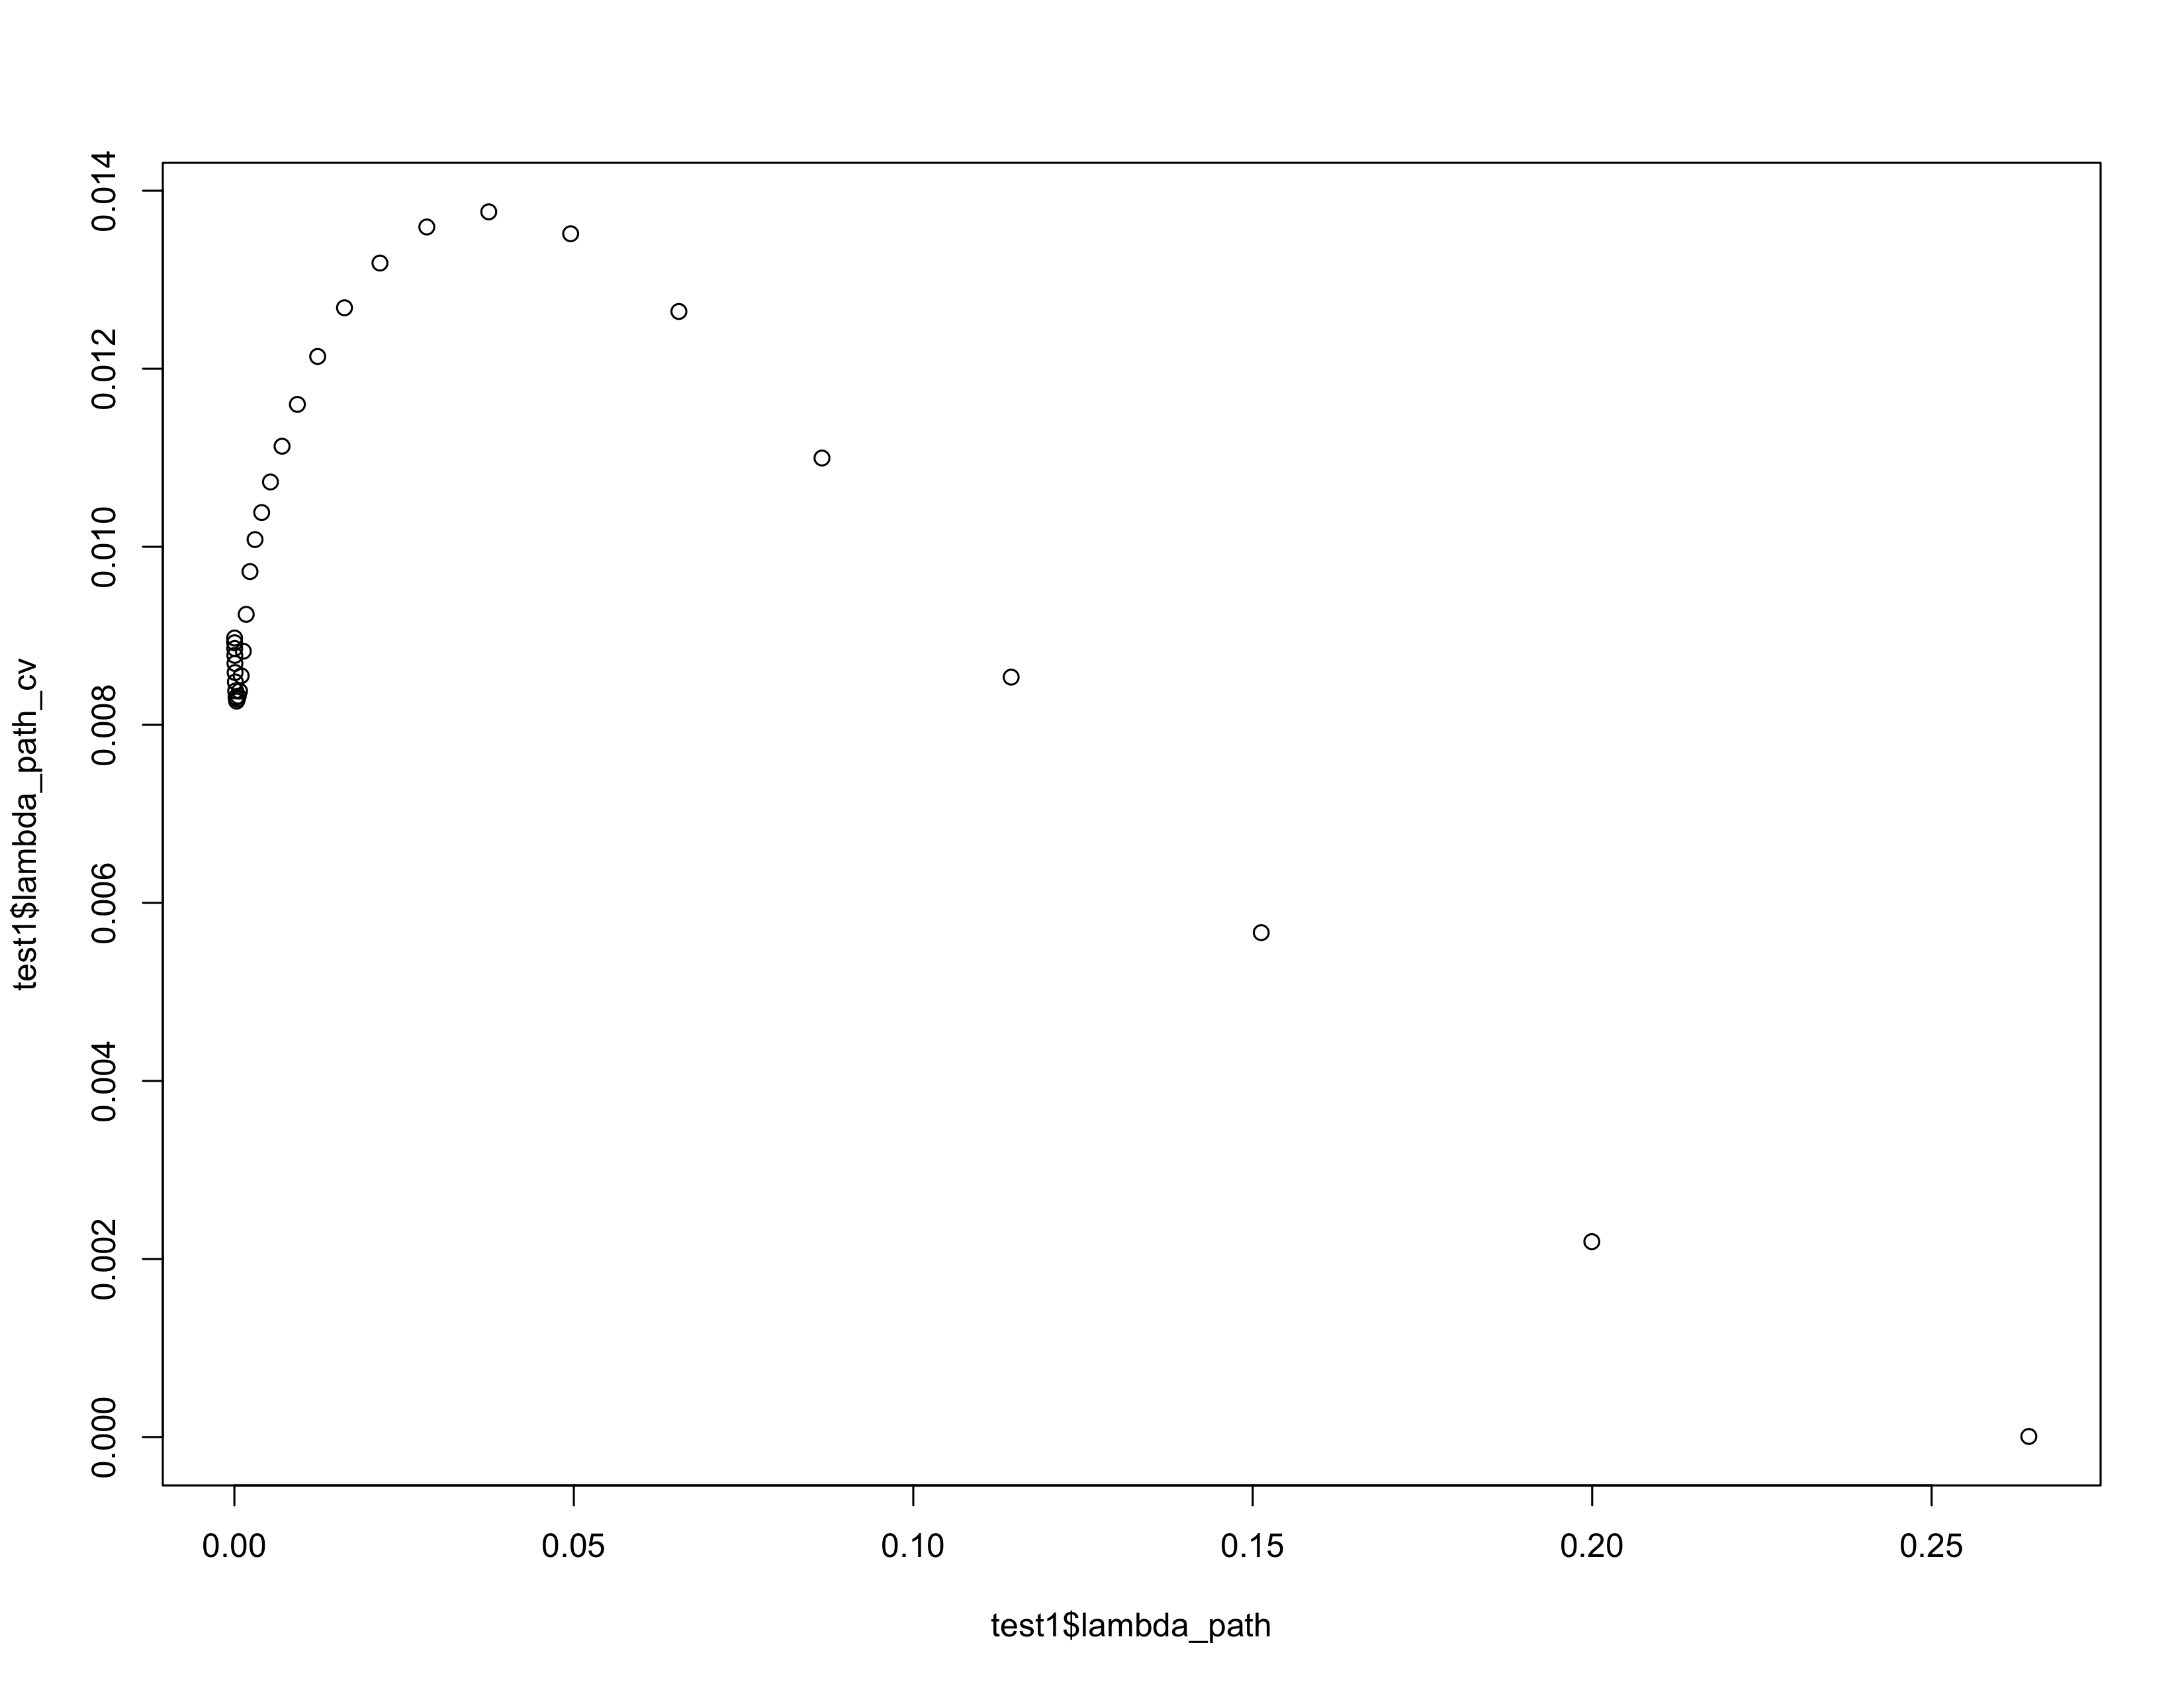
\includegraphics[width=1\linewidth]{./result_plot/ll_use_k/2wrong_path_plot}
\end{subfigure}

\end{figure}

\begin{figure}[H]
\centering
\begin{subfigure}{0.5\textwidth}
  \centering
  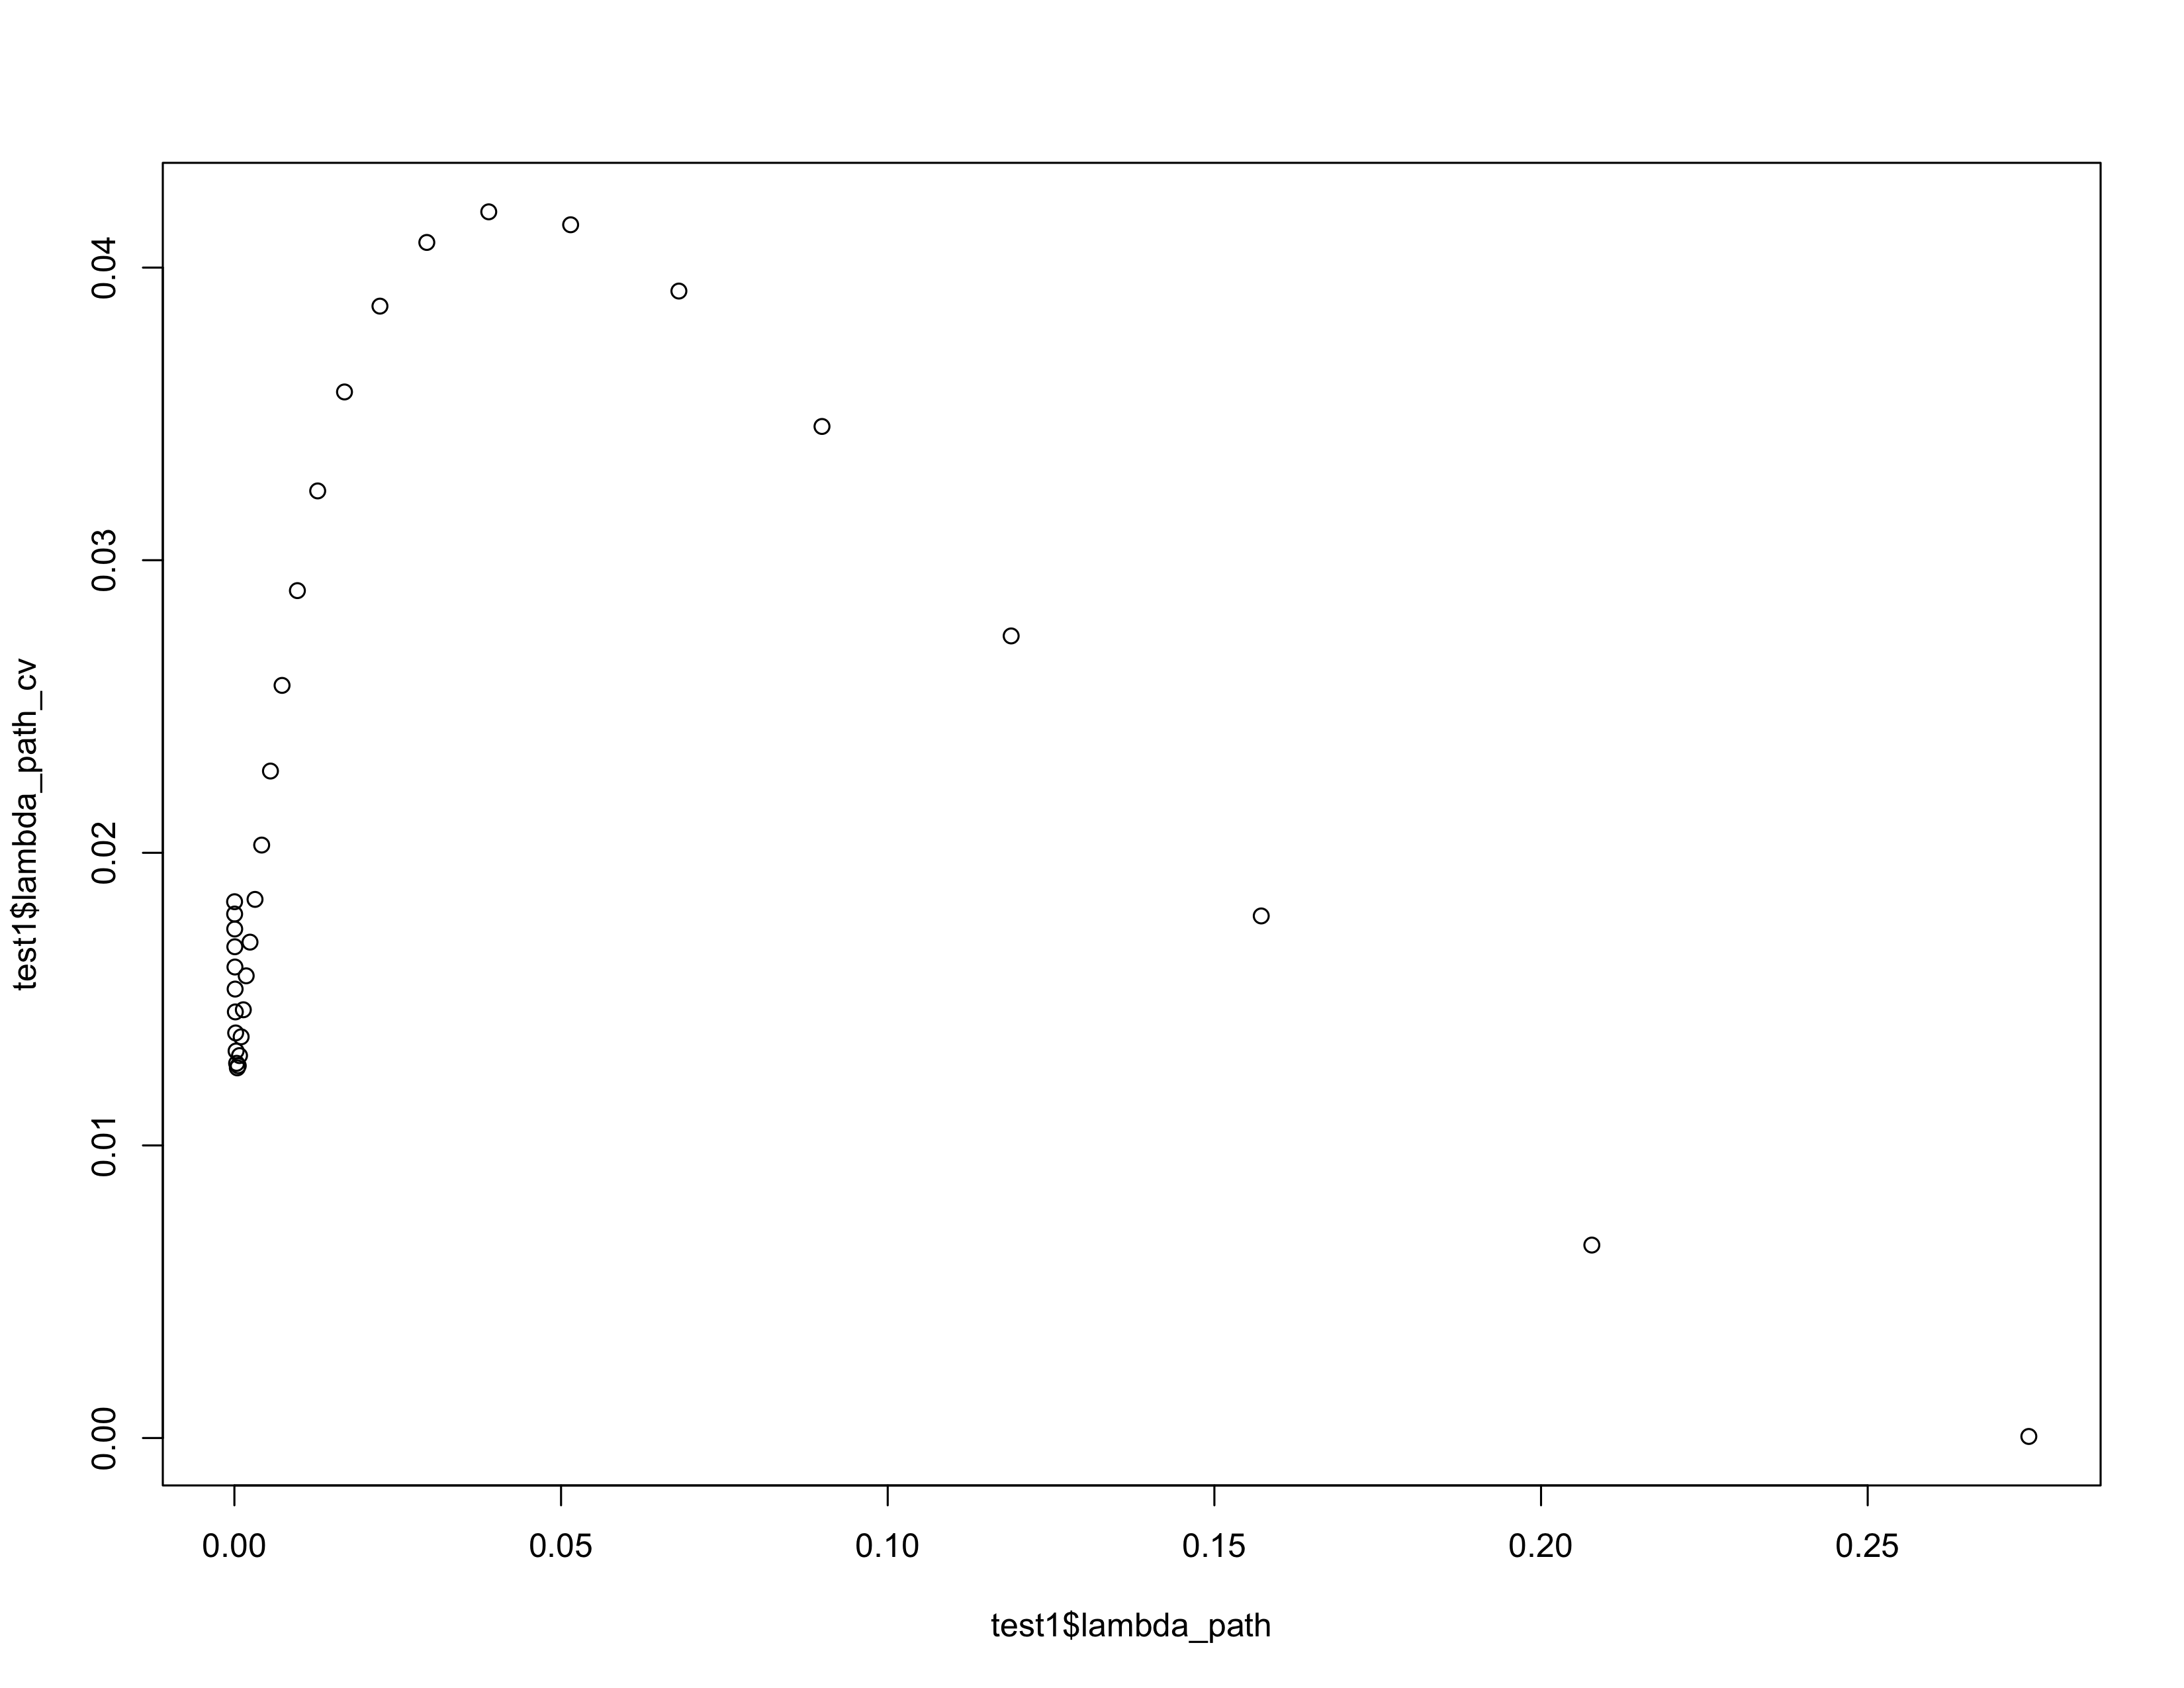
\includegraphics[width=1\linewidth]{./result_plot/ll_use_k/3wrong_path_plot}
\end{subfigure}%
\begin{subfigure}{.5\textwidth}
  \centering
  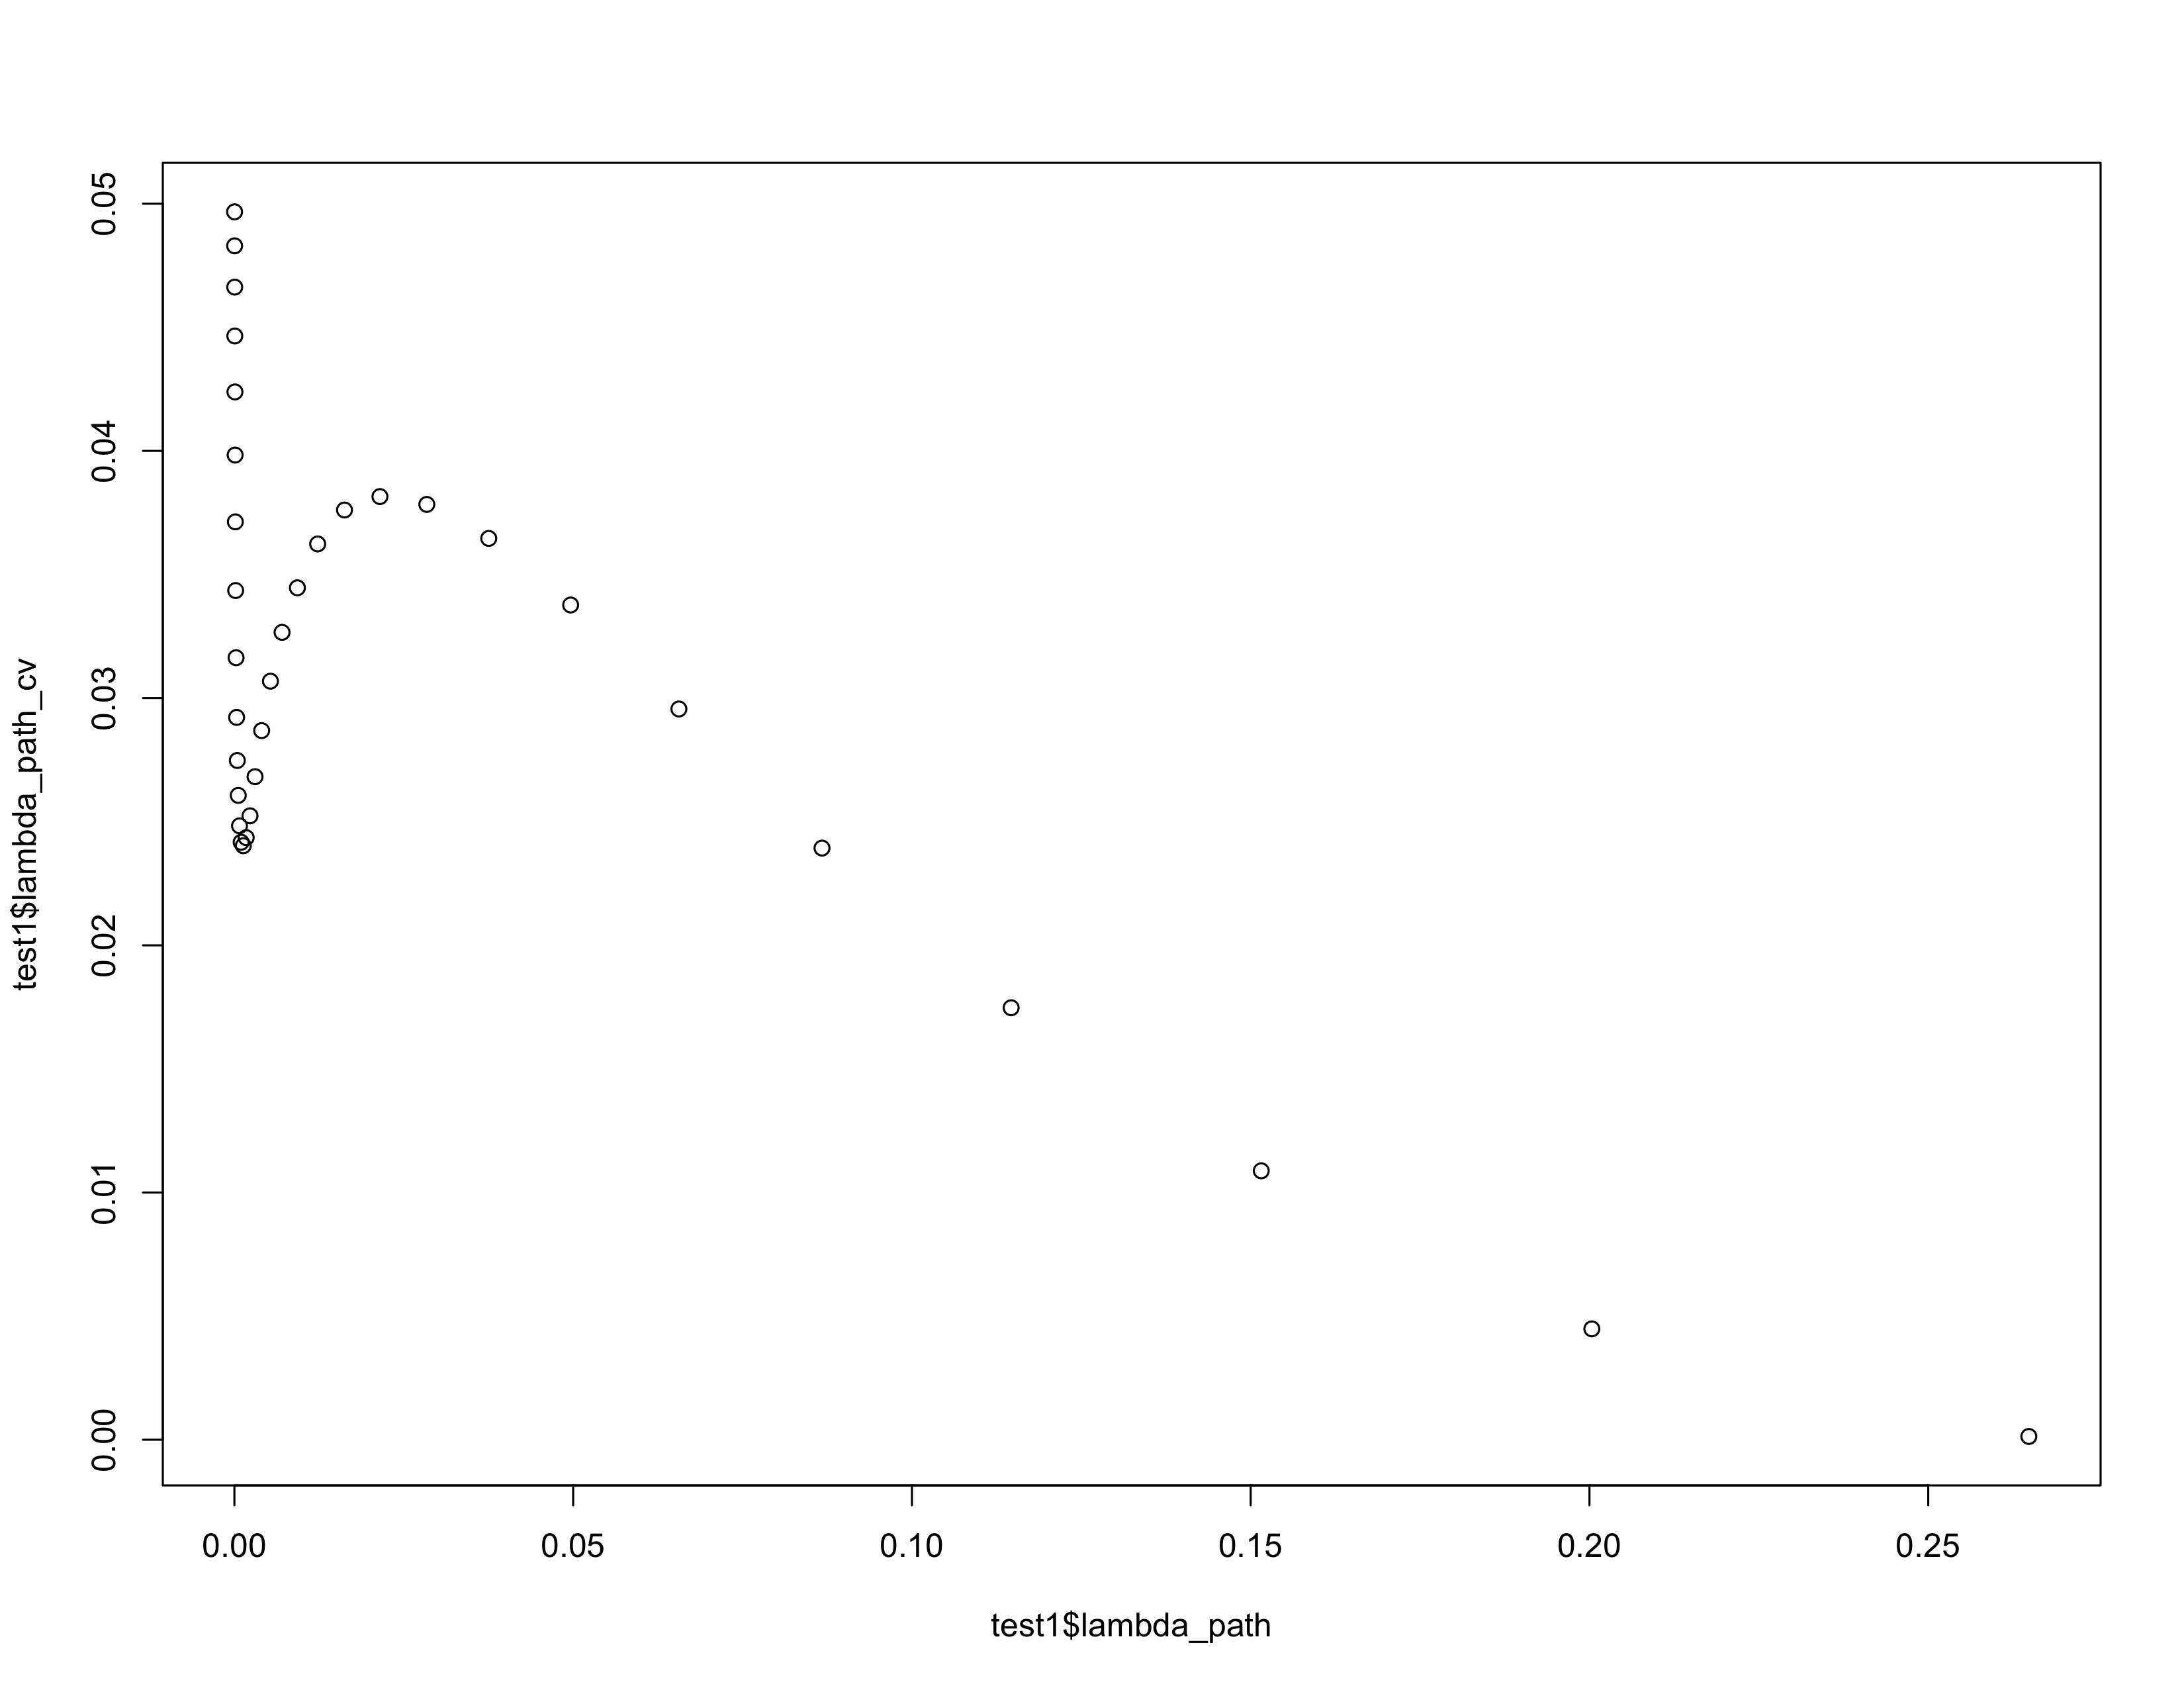
\includegraphics[width=1\linewidth]{./result_plot/ll_use_k/4wrong_path_plot}
\end{subfigure}

\end{figure}

\begin{figure}[H]
\centering
\begin{subfigure}{0.5\textwidth}
  \centering
  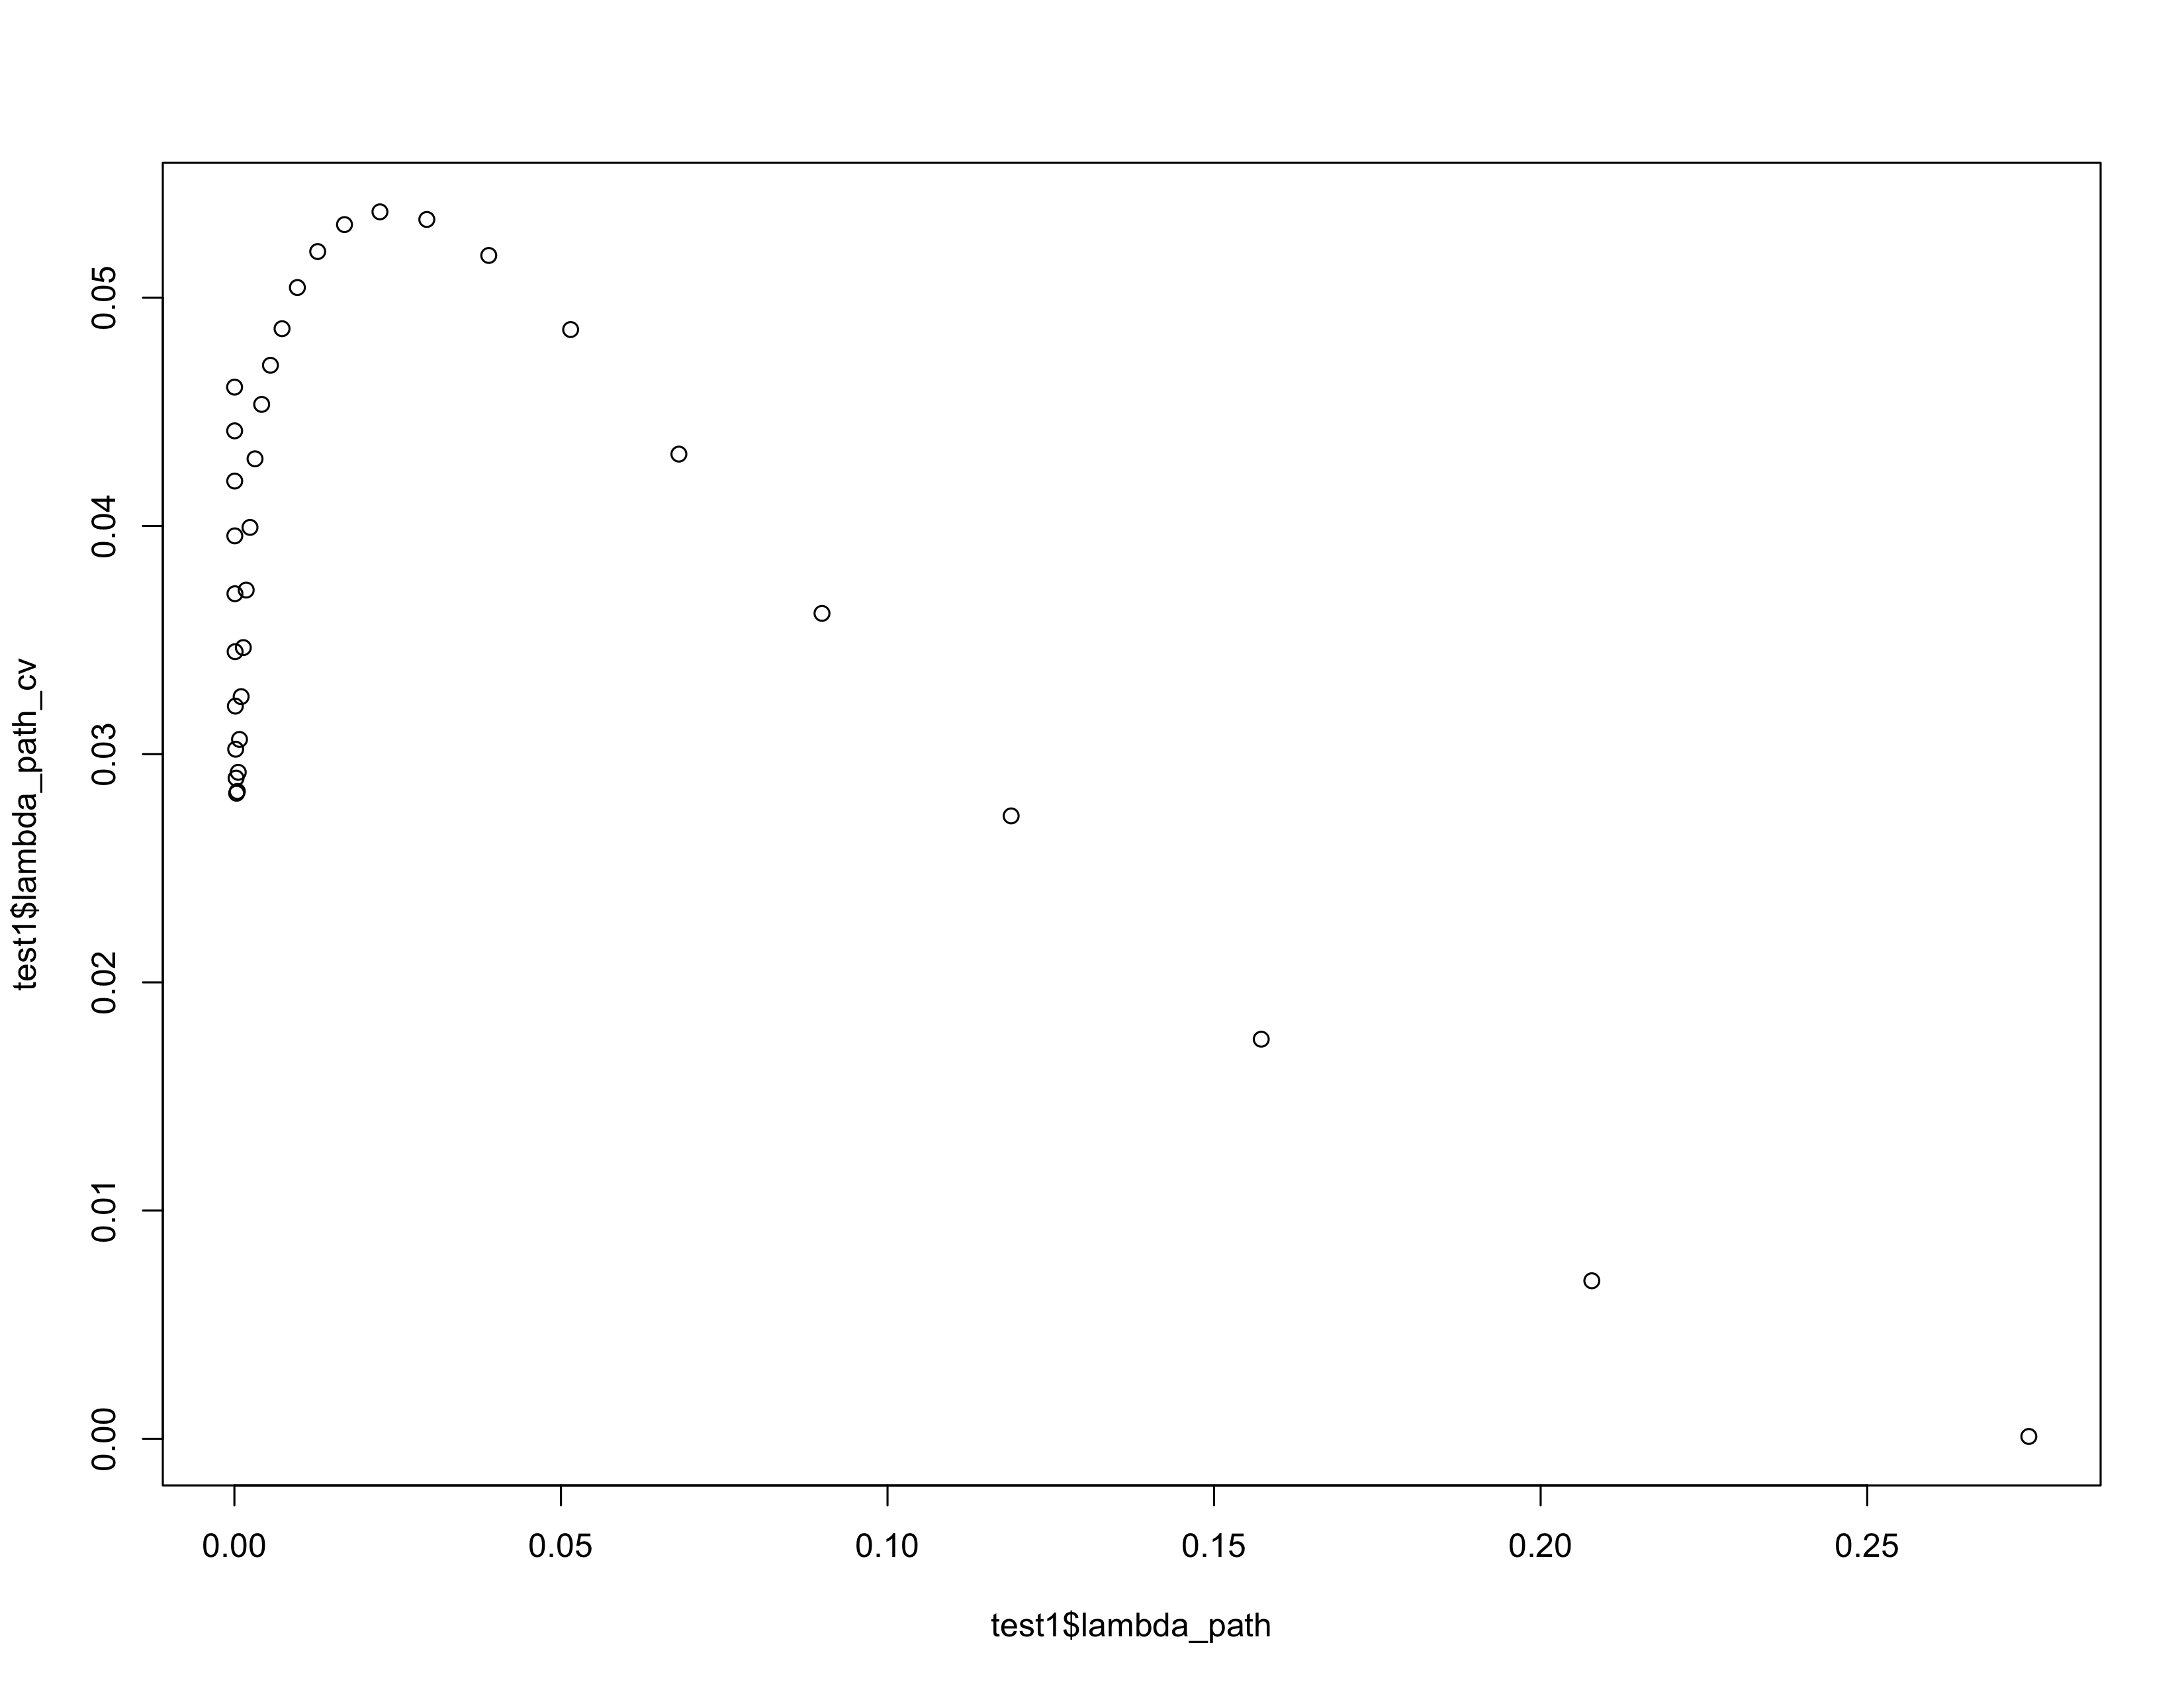
\includegraphics[width=1\linewidth]{./result_plot/ll_use_k/5wrong_path_plot}
\end{subfigure}%
\begin{subfigure}{.5\textwidth}
  \centering
  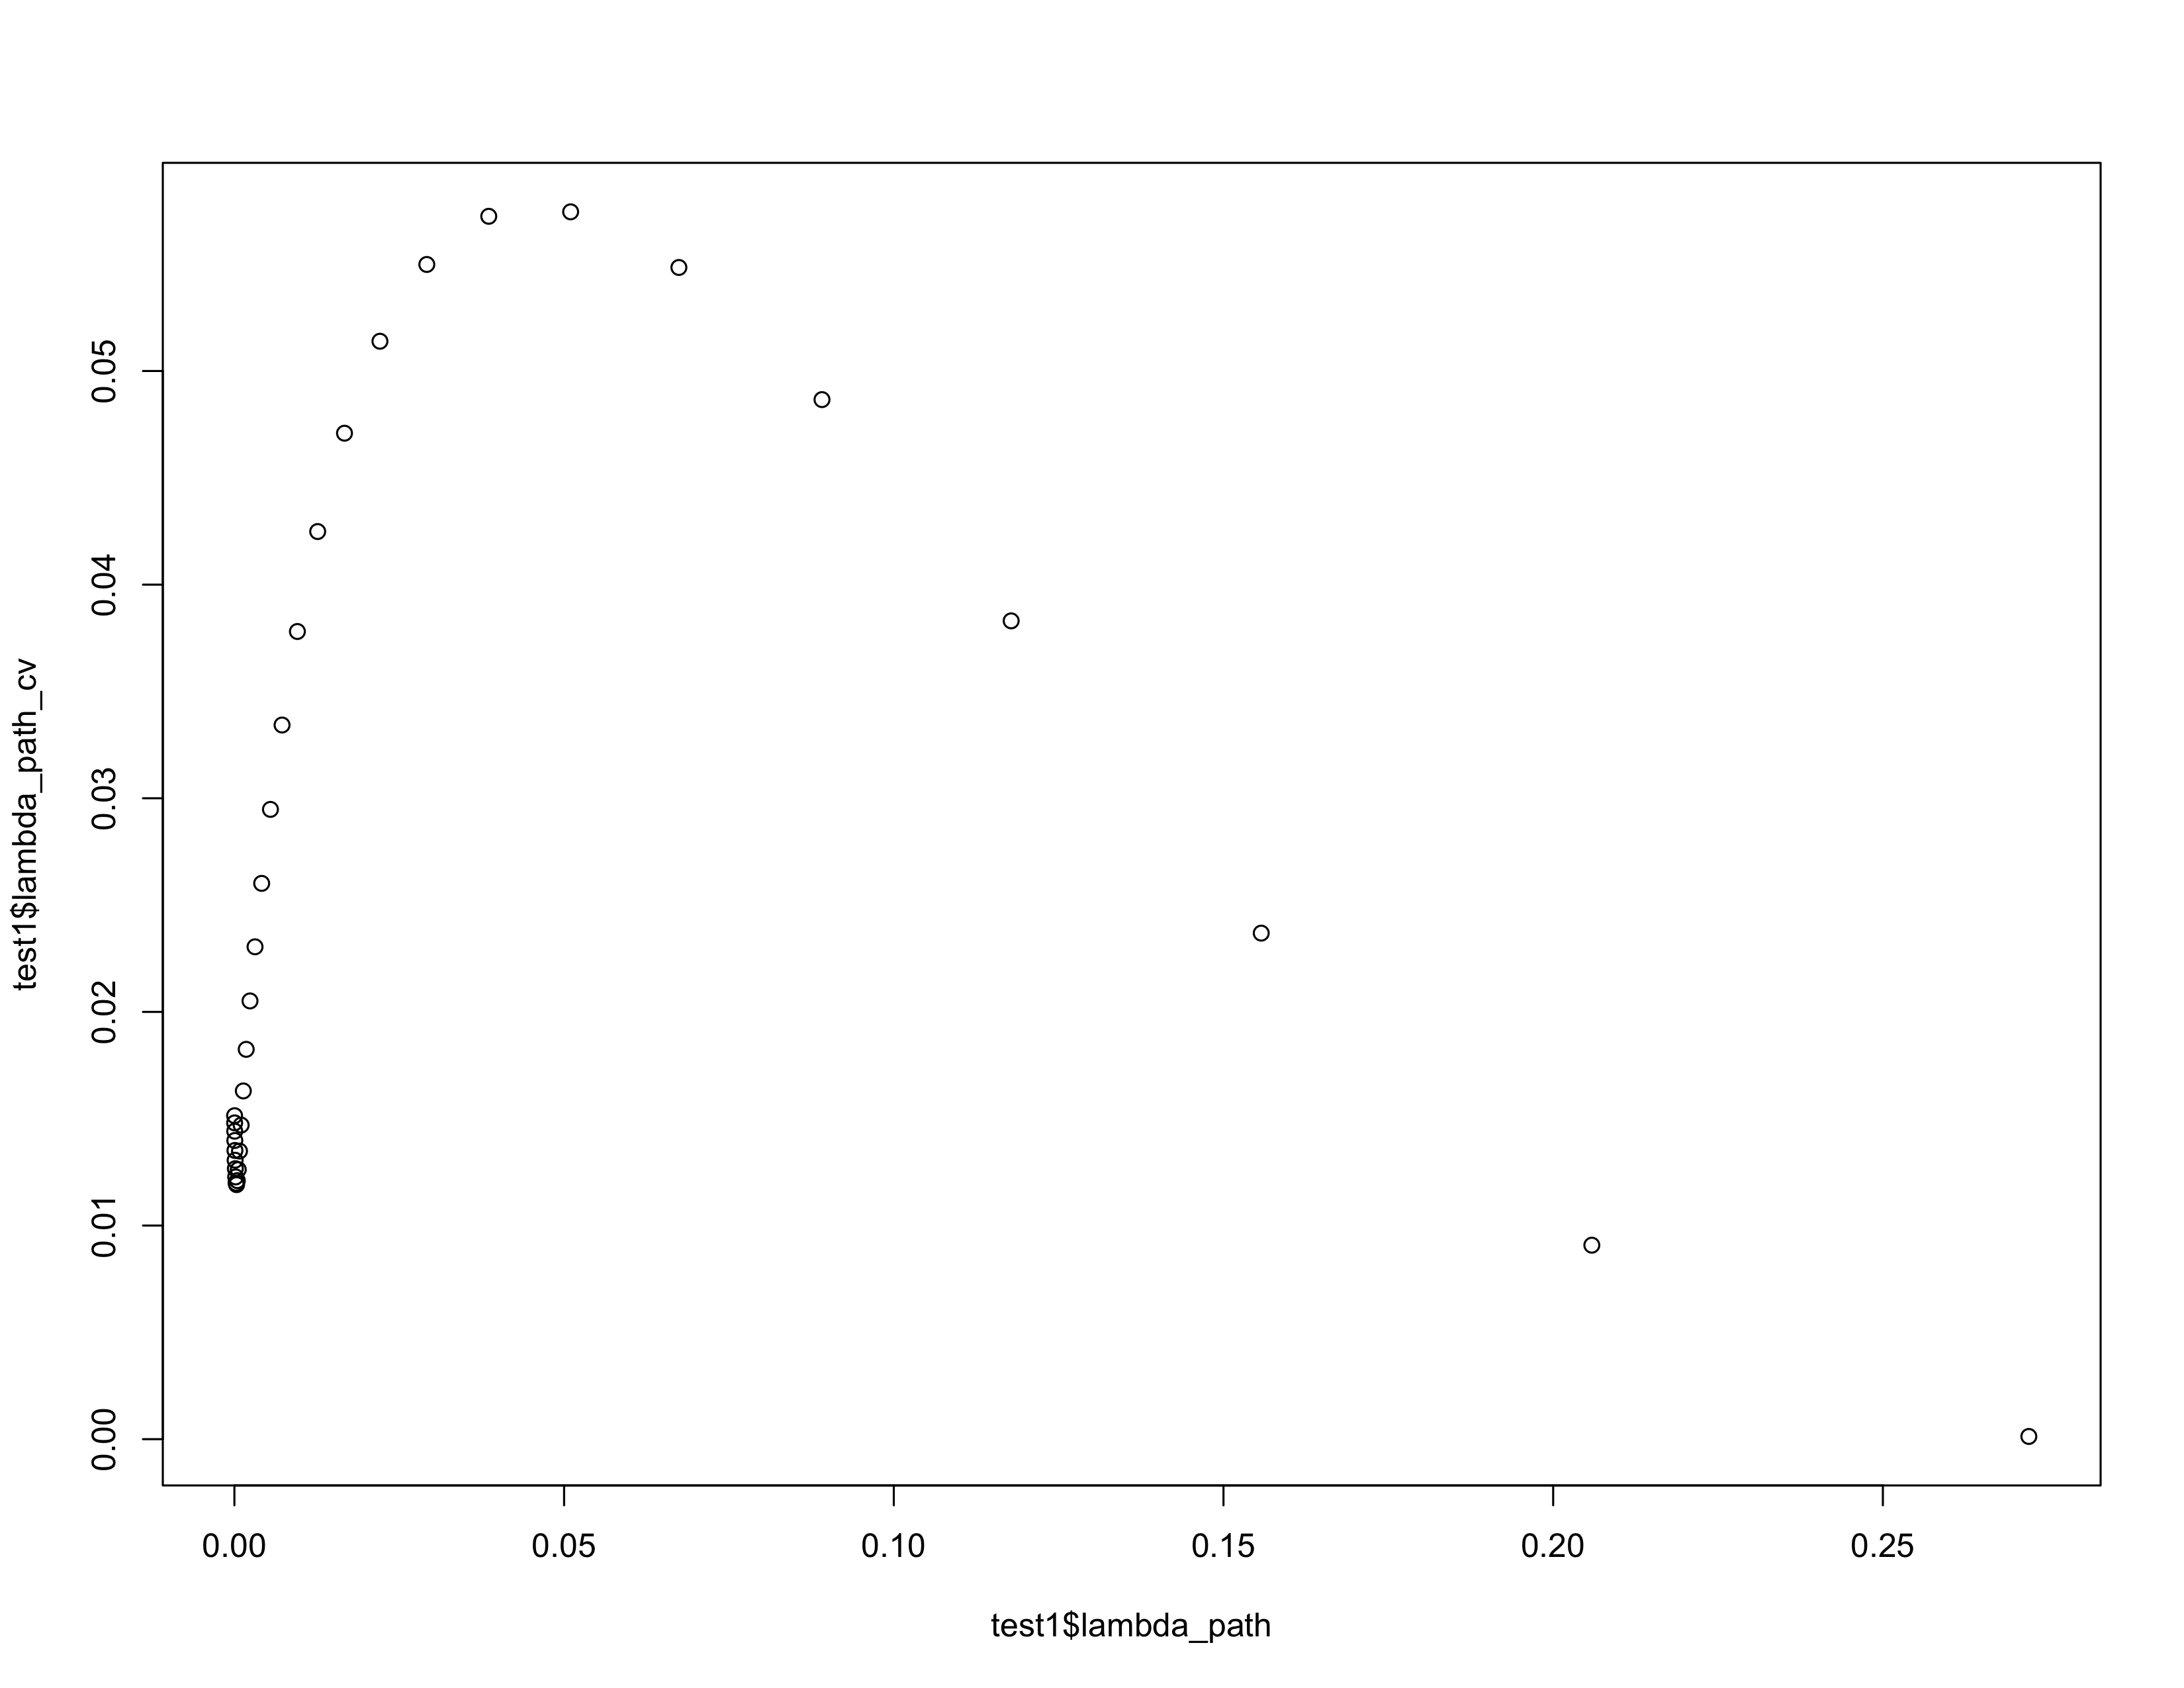
\includegraphics[width=1\linewidth]{./result_plot/ll_use_k/6wrong_path_plot}
\end{subfigure}

\end{figure}

\begin{figure}[H]
\centering
\begin{subfigure}{0.5\textwidth}
  \centering
  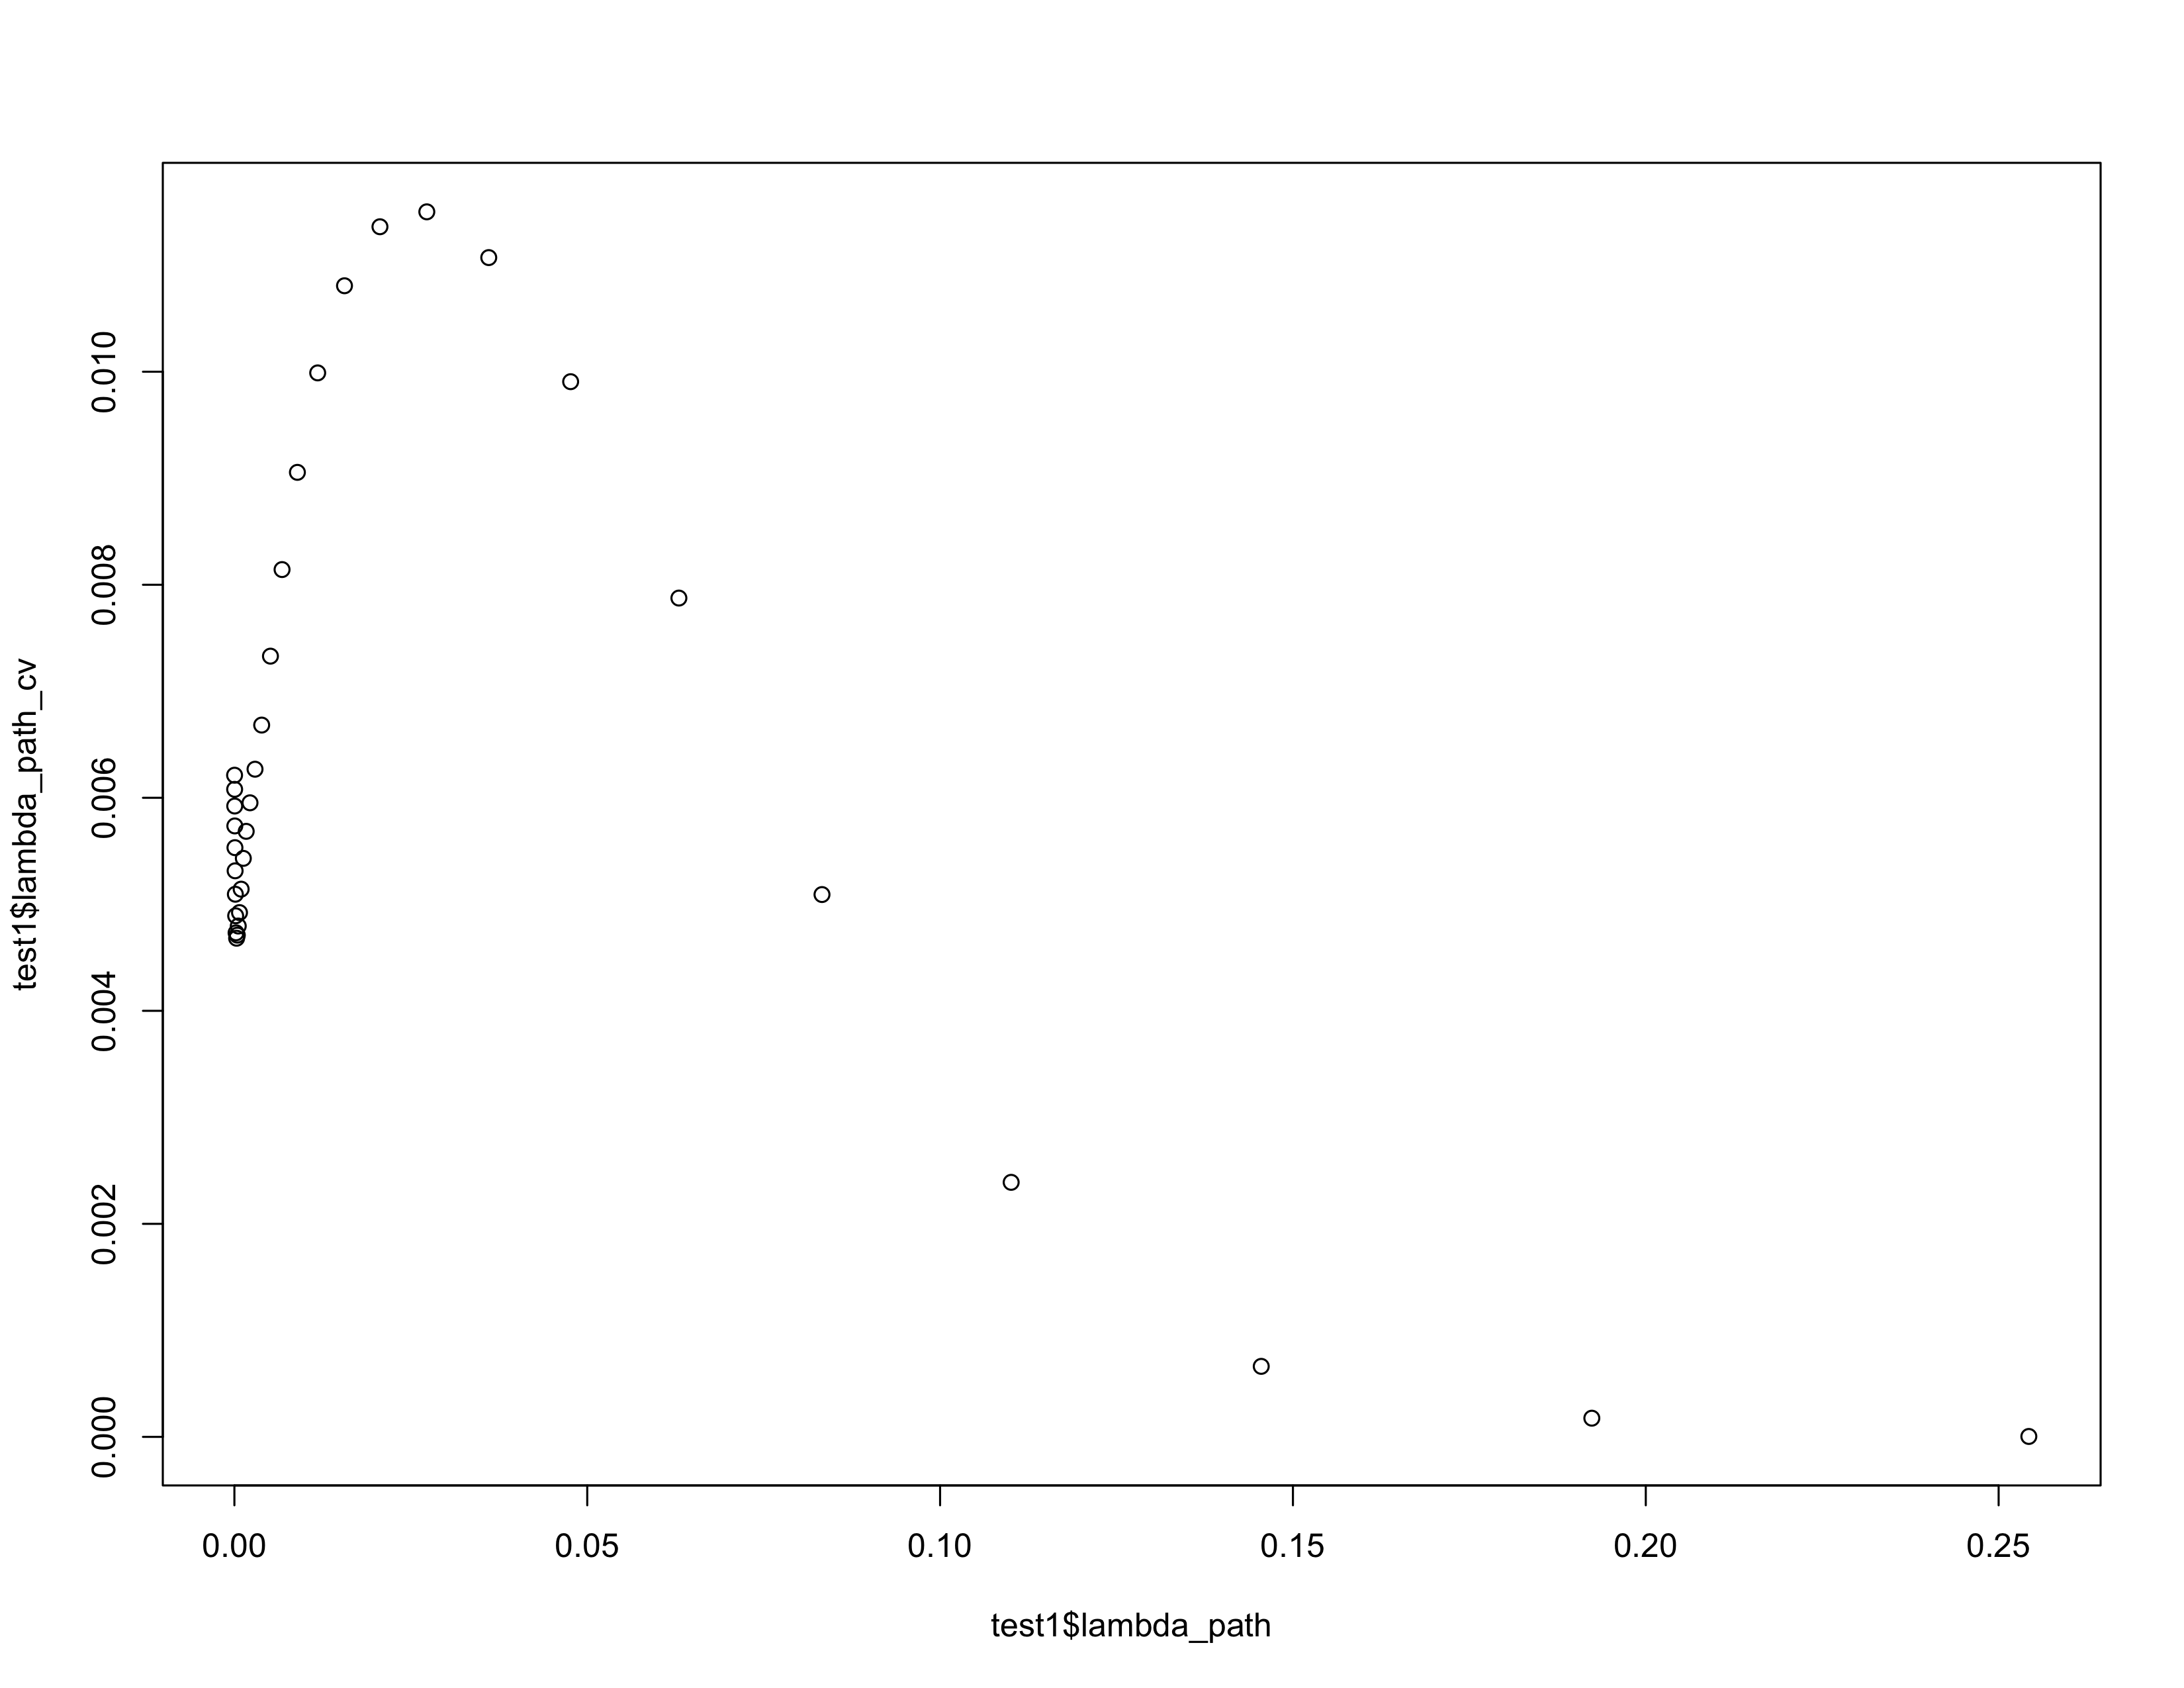
\includegraphics[width=1\linewidth]{./result_plot/ll_use_k/7wrong_path_plot}
\end{subfigure}%
\begin{subfigure}{.5\textwidth}
  \centering
  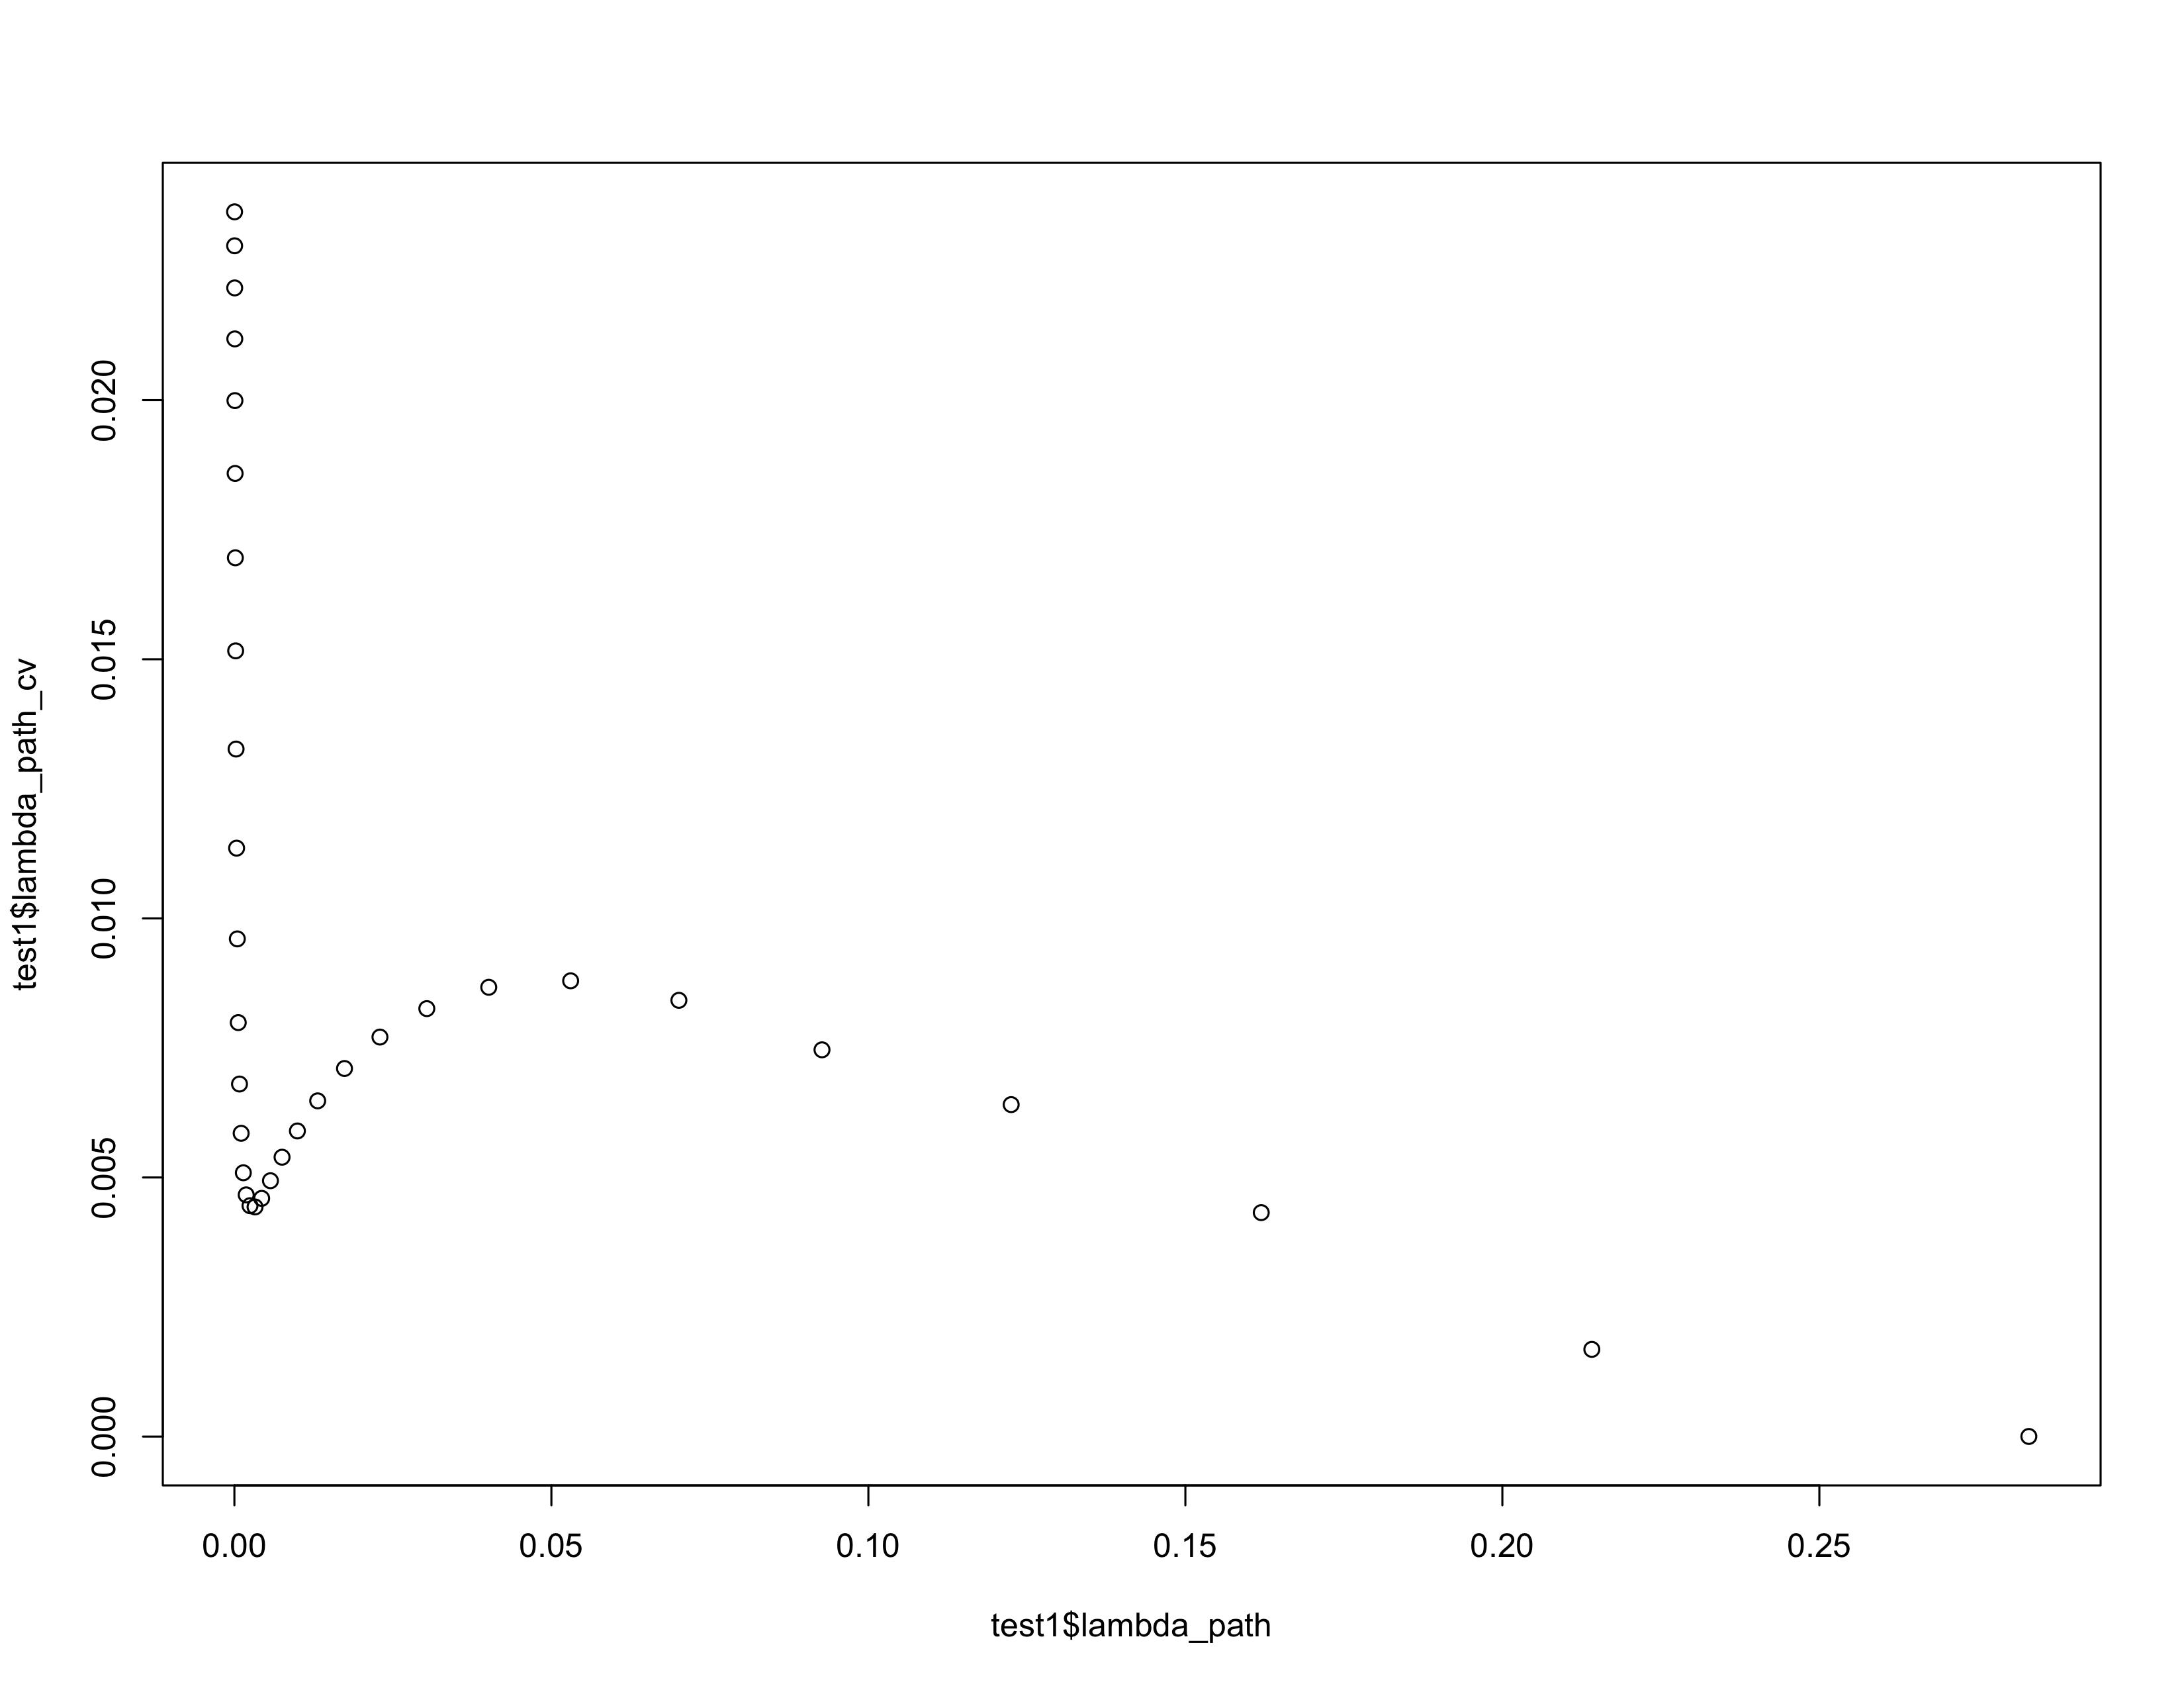
\includegraphics[width=1\linewidth]{./result_plot/ll_use_k/8wrong_path_plot}
\end{subfigure}

\end{figure}

\begin{figure}[H]
\centering
\begin{subfigure}{0.5\textwidth}
  \centering
  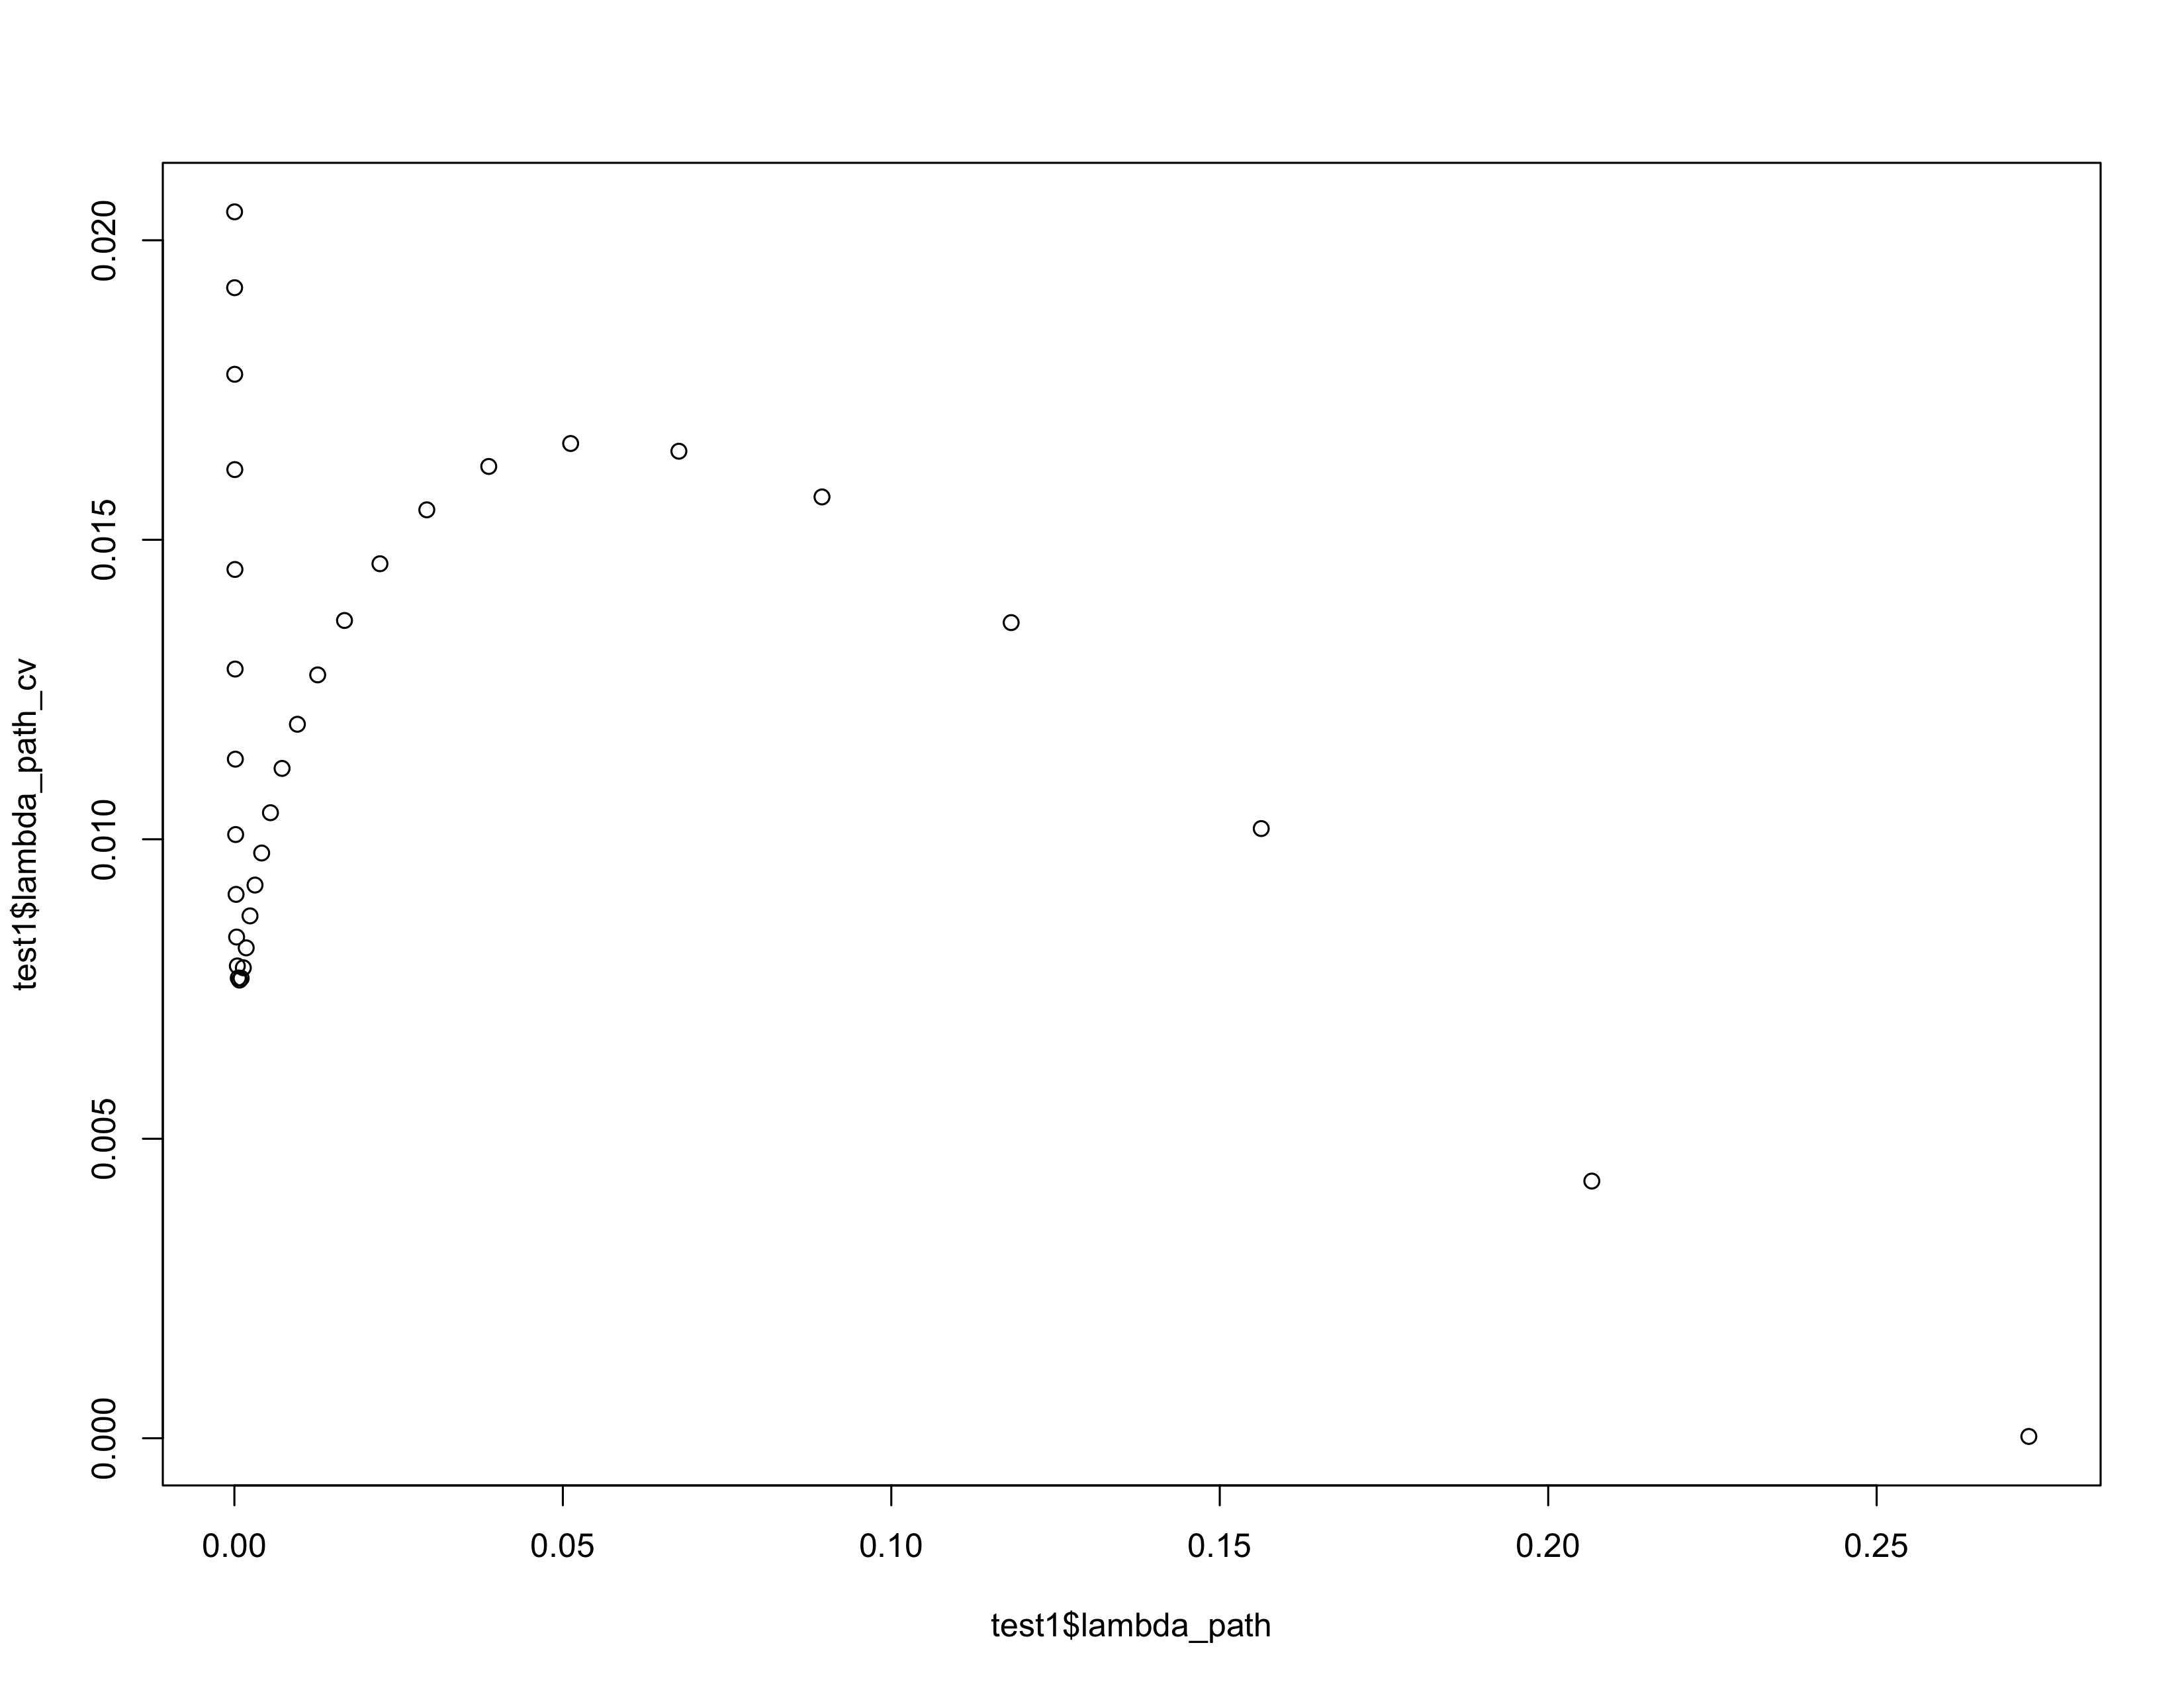
\includegraphics[width=1\linewidth]{./result_plot/ll_use_k/9wrong_path_plot}
\end{subfigure}%
\begin{subfigure}{.5\textwidth}
  \centering
  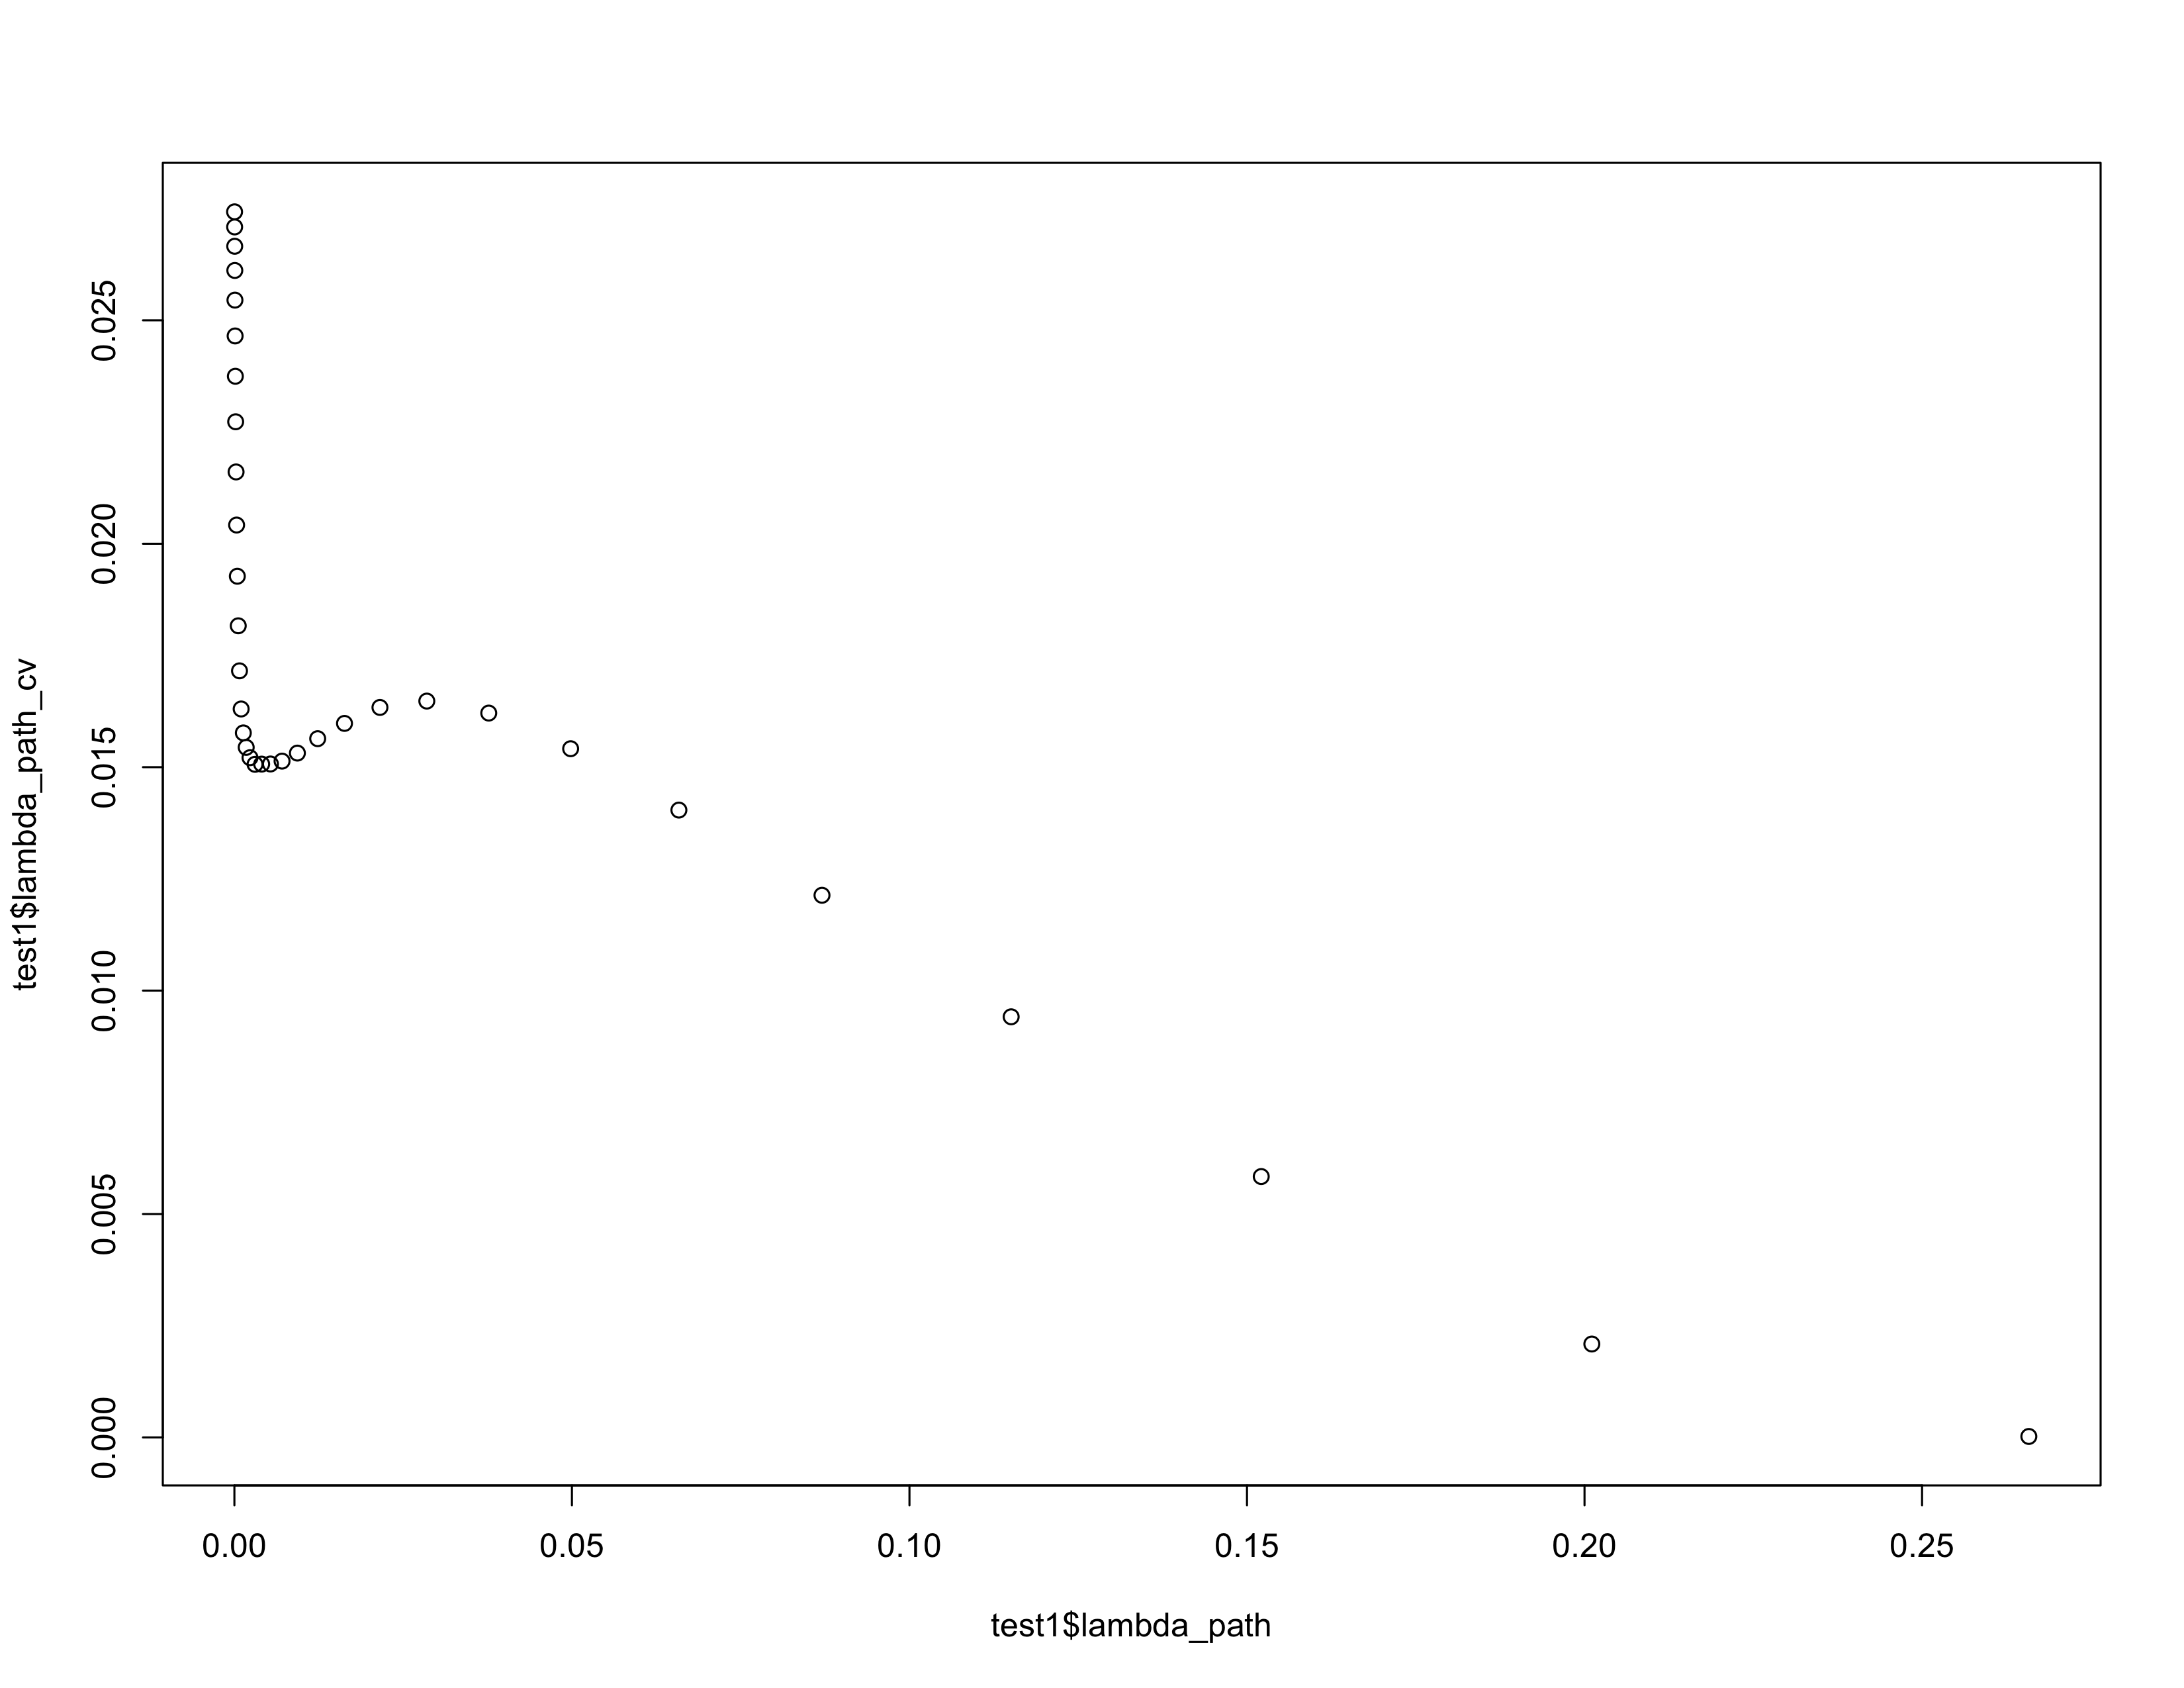
\includegraphics[width=1\linewidth]{./result_plot/ll_use_k/10wrong_path_plot}
\end{subfigure}

\end{figure}

\section{square sum term}
\label{sec:square}
In this part, I tried use the squared term in our sum formulation.
In this section, we define:
$$
\argmin_{\lambda}\text{cv}(\lambda)=\argmin_{\lambda}\sum_{k=1}^5\{l(\hat{\beta}_\lambda^{(-k)})-l^{(-k)}\hat{\beta}_(\lambda^{(-k)})\}^2
$$
The plots we got are

\begin{figure}[H]
\centering
\begin{subfigure}{0.5\textwidth}
  \centering
  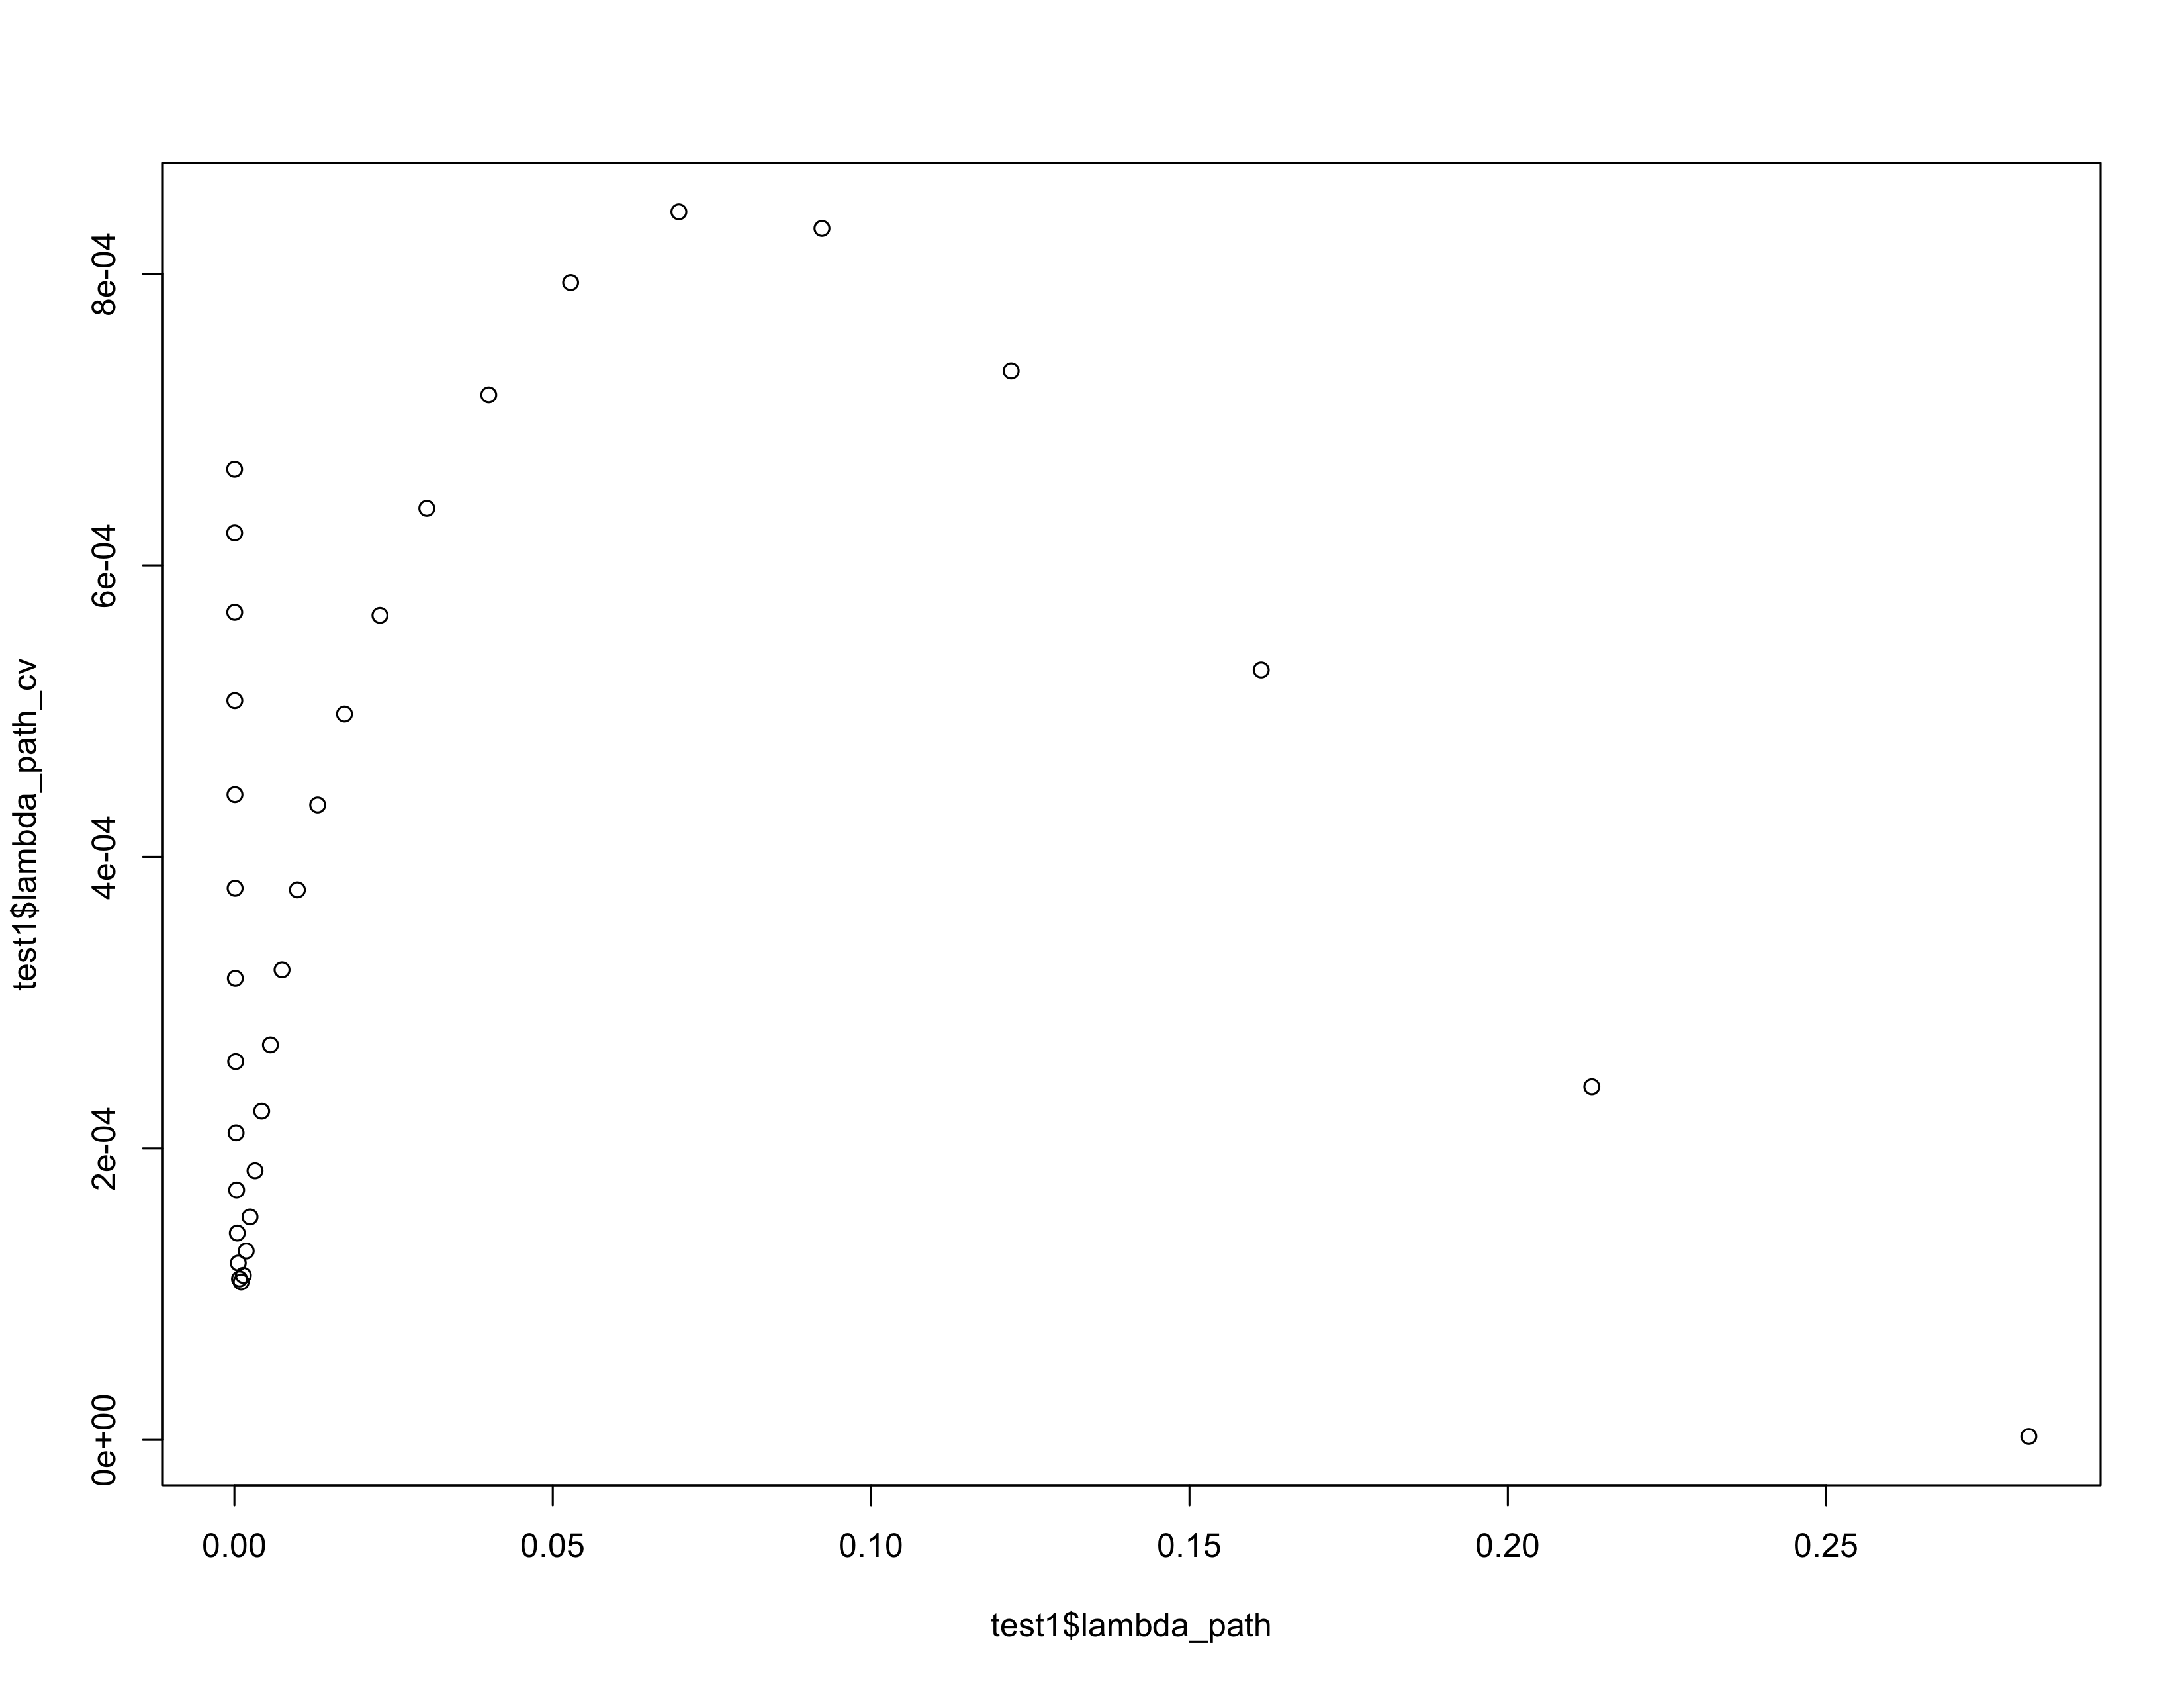
\includegraphics[width=1\linewidth]{./result_plot/cv_square/1wrong_path_plot}
\end{subfigure}%
\begin{subfigure}{.5\textwidth}
  \centering
  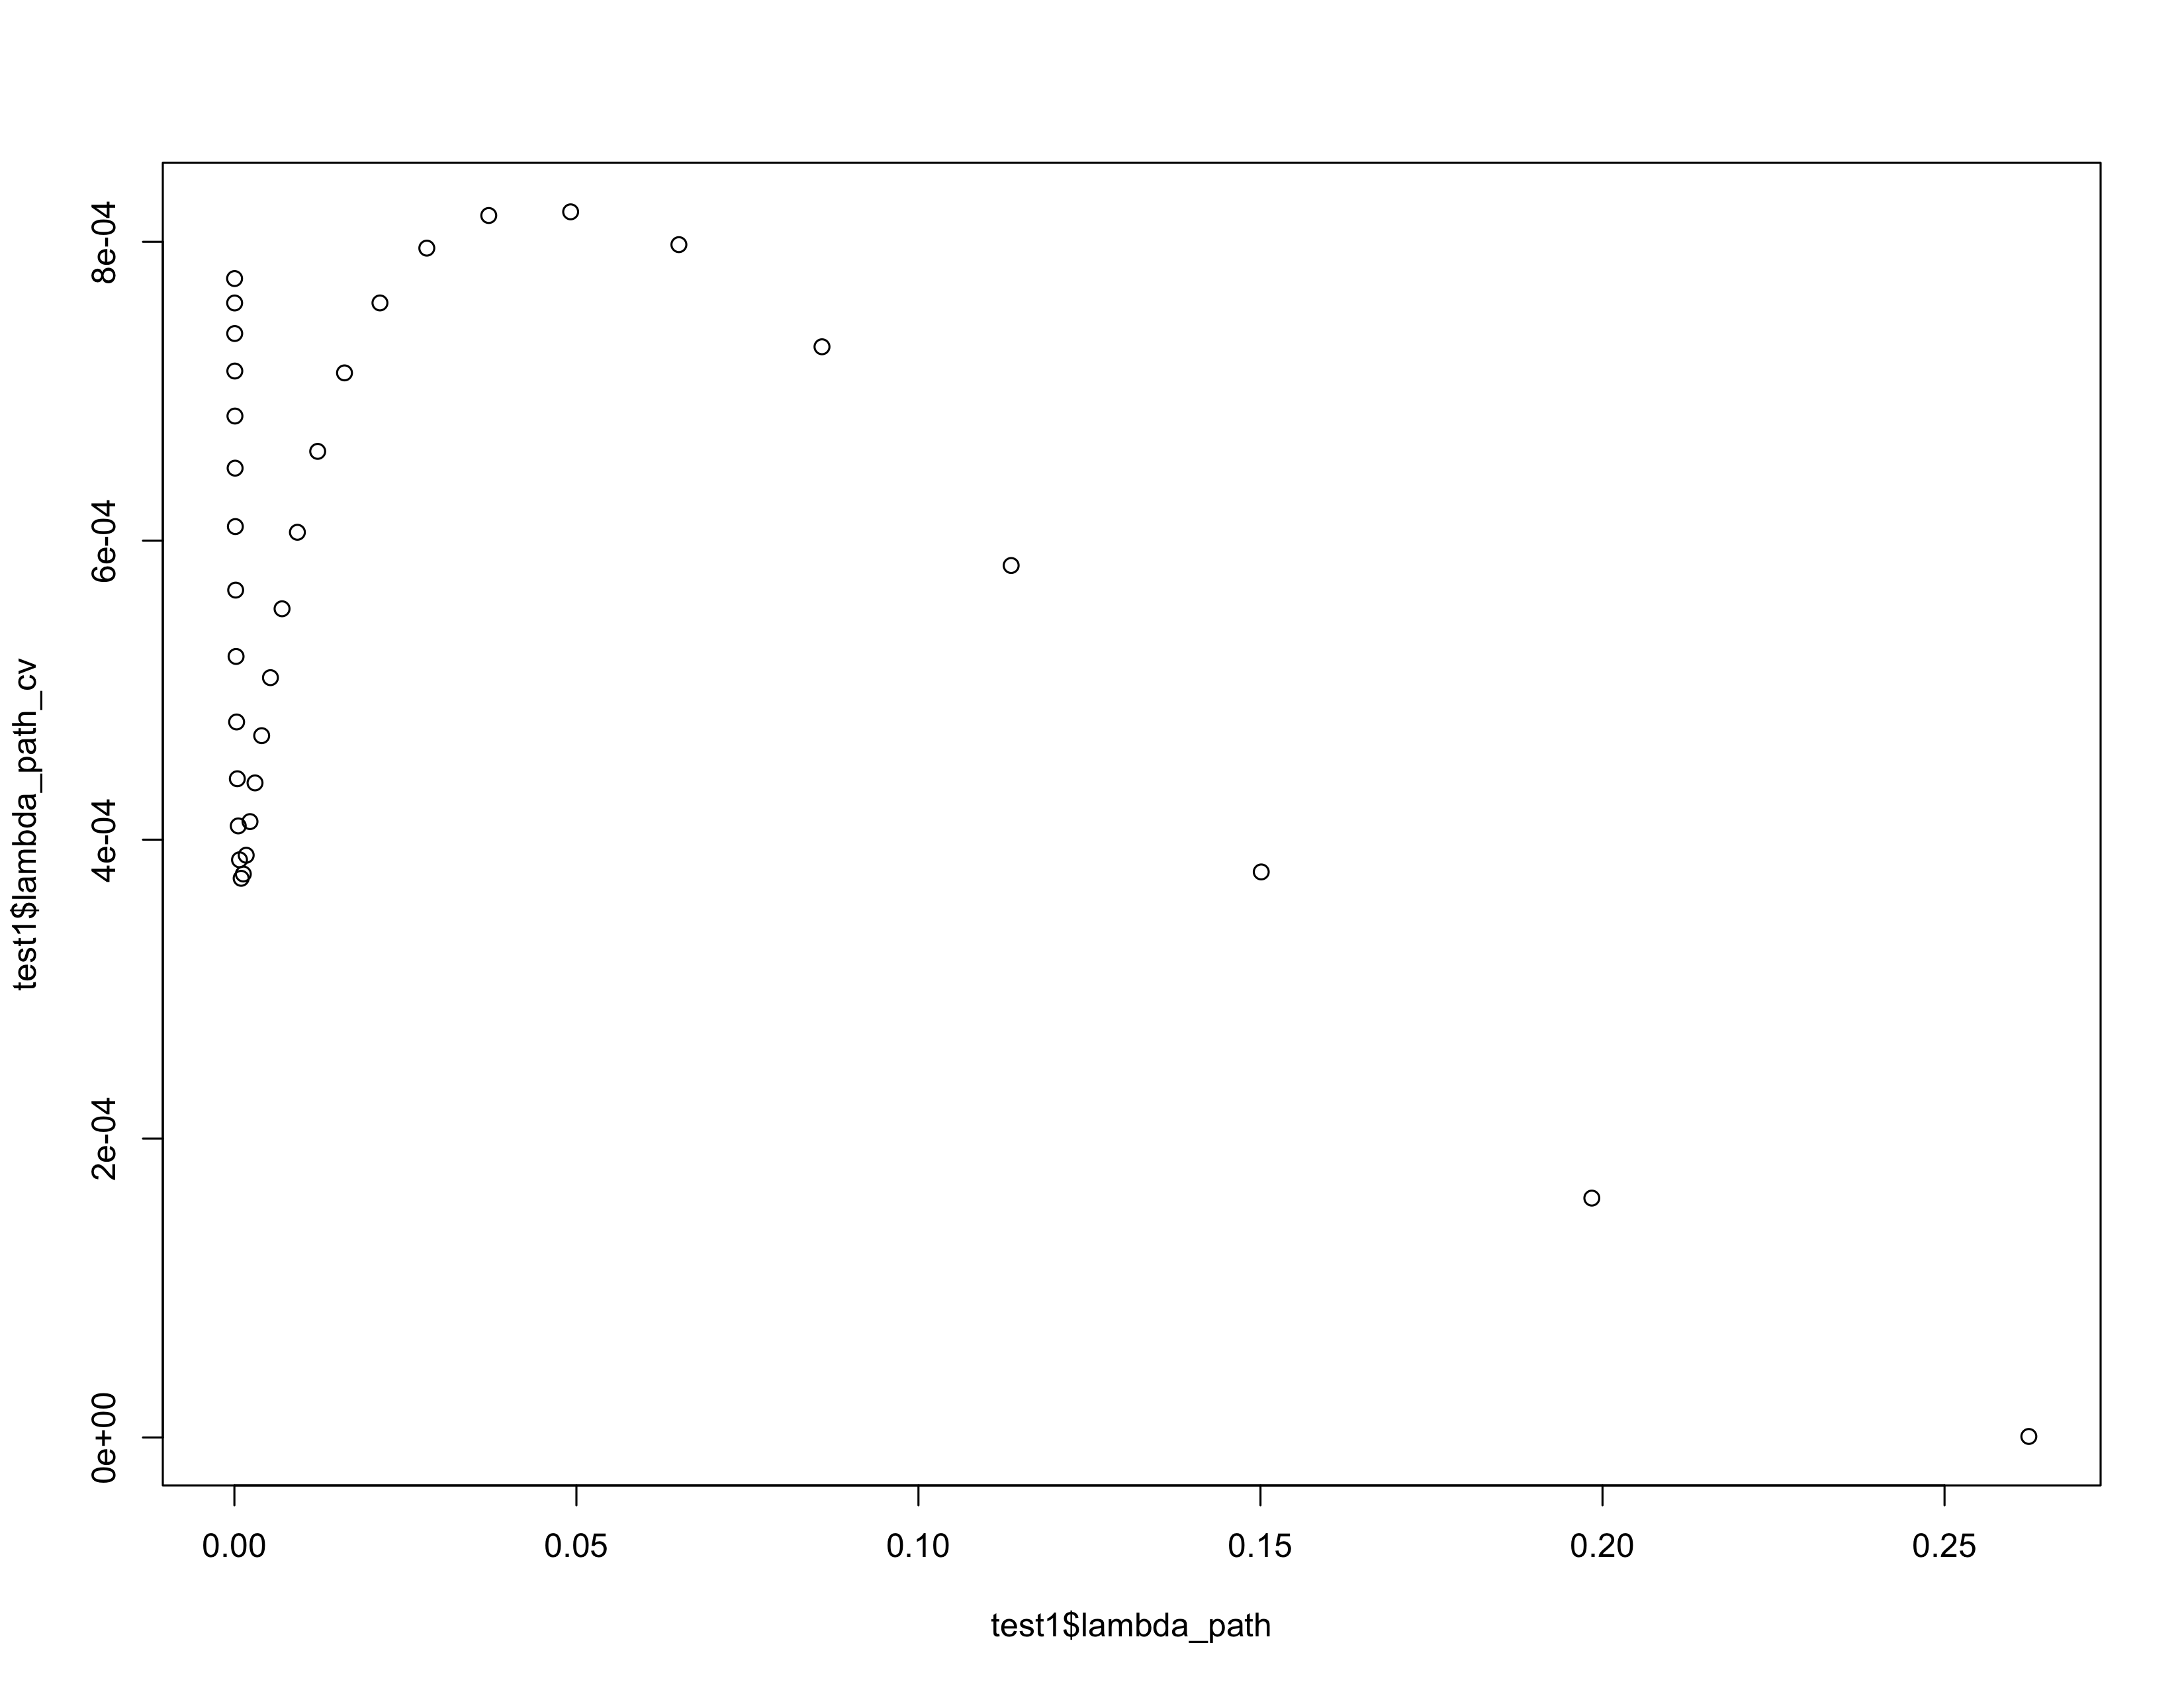
\includegraphics[width=1\linewidth]{./result_plot/cv_square/2wrong_path_plot}
\end{subfigure}

\end{figure}

\begin{figure}[H]
\centering
\begin{subfigure}{0.5\textwidth}
  \centering
  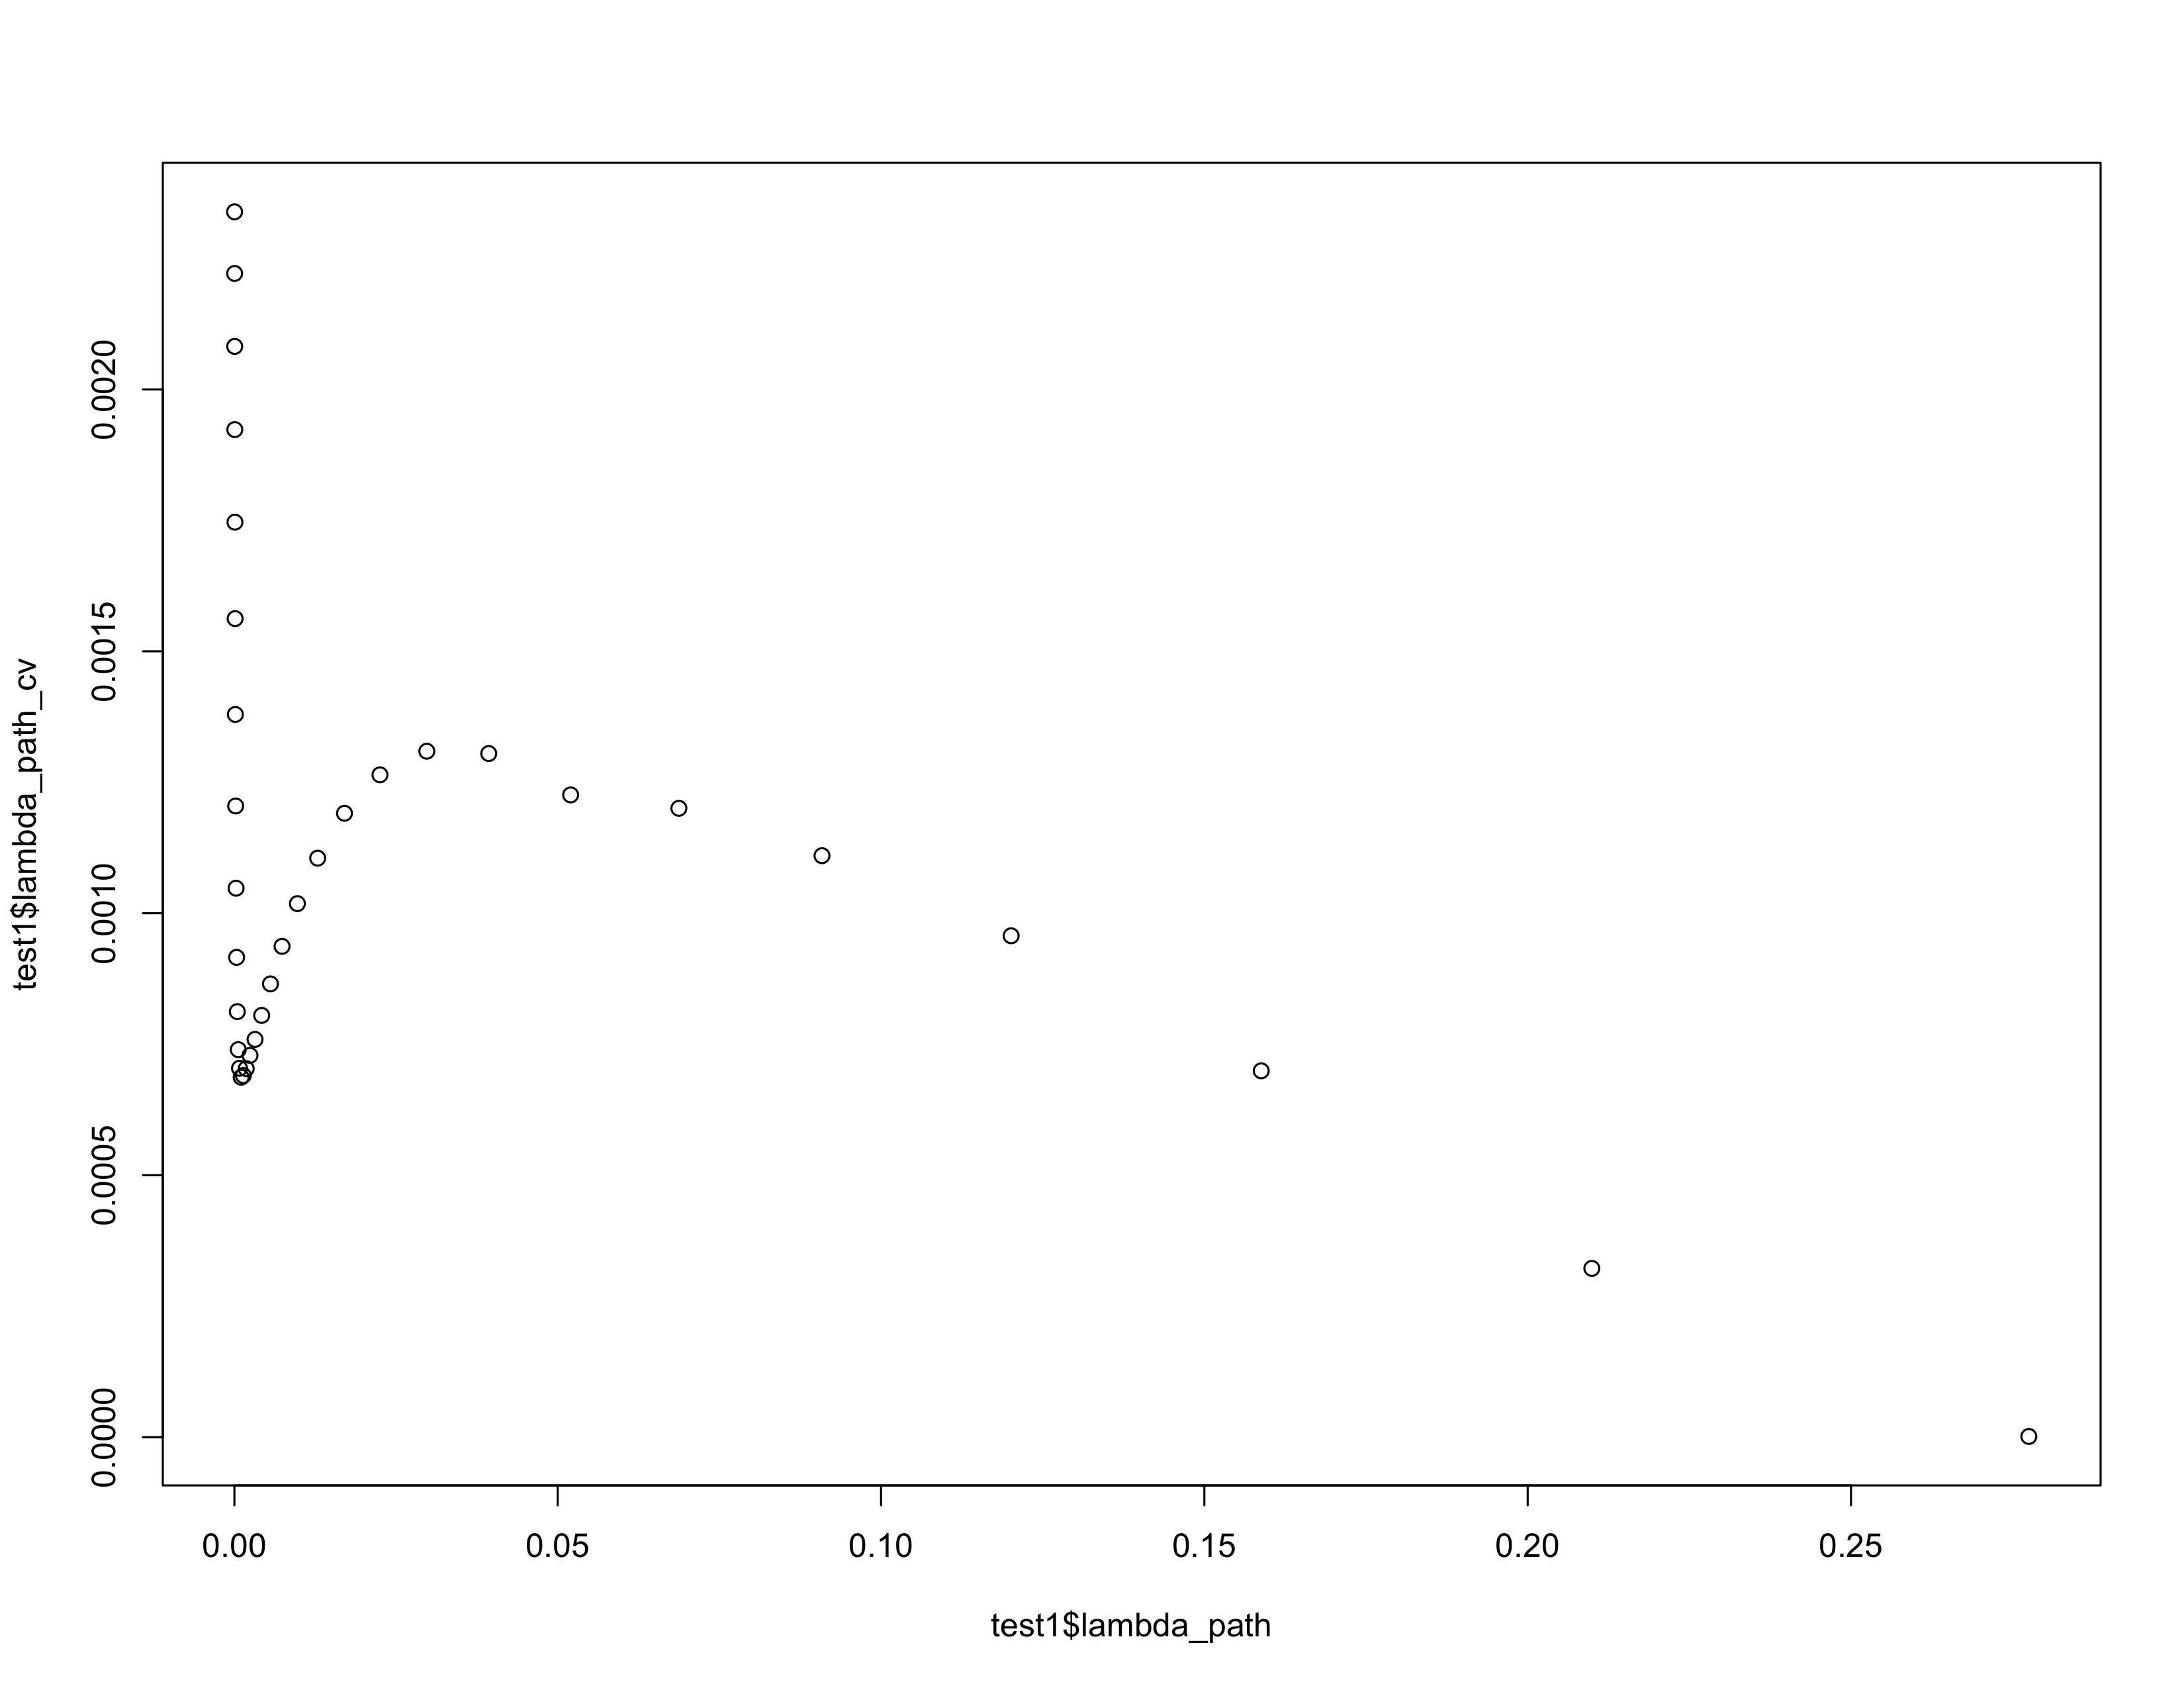
\includegraphics[width=1\linewidth]{./result_plot/cv_square/3wrong_path_plot}
\end{subfigure}%
\begin{subfigure}{.5\textwidth}
  \centering
  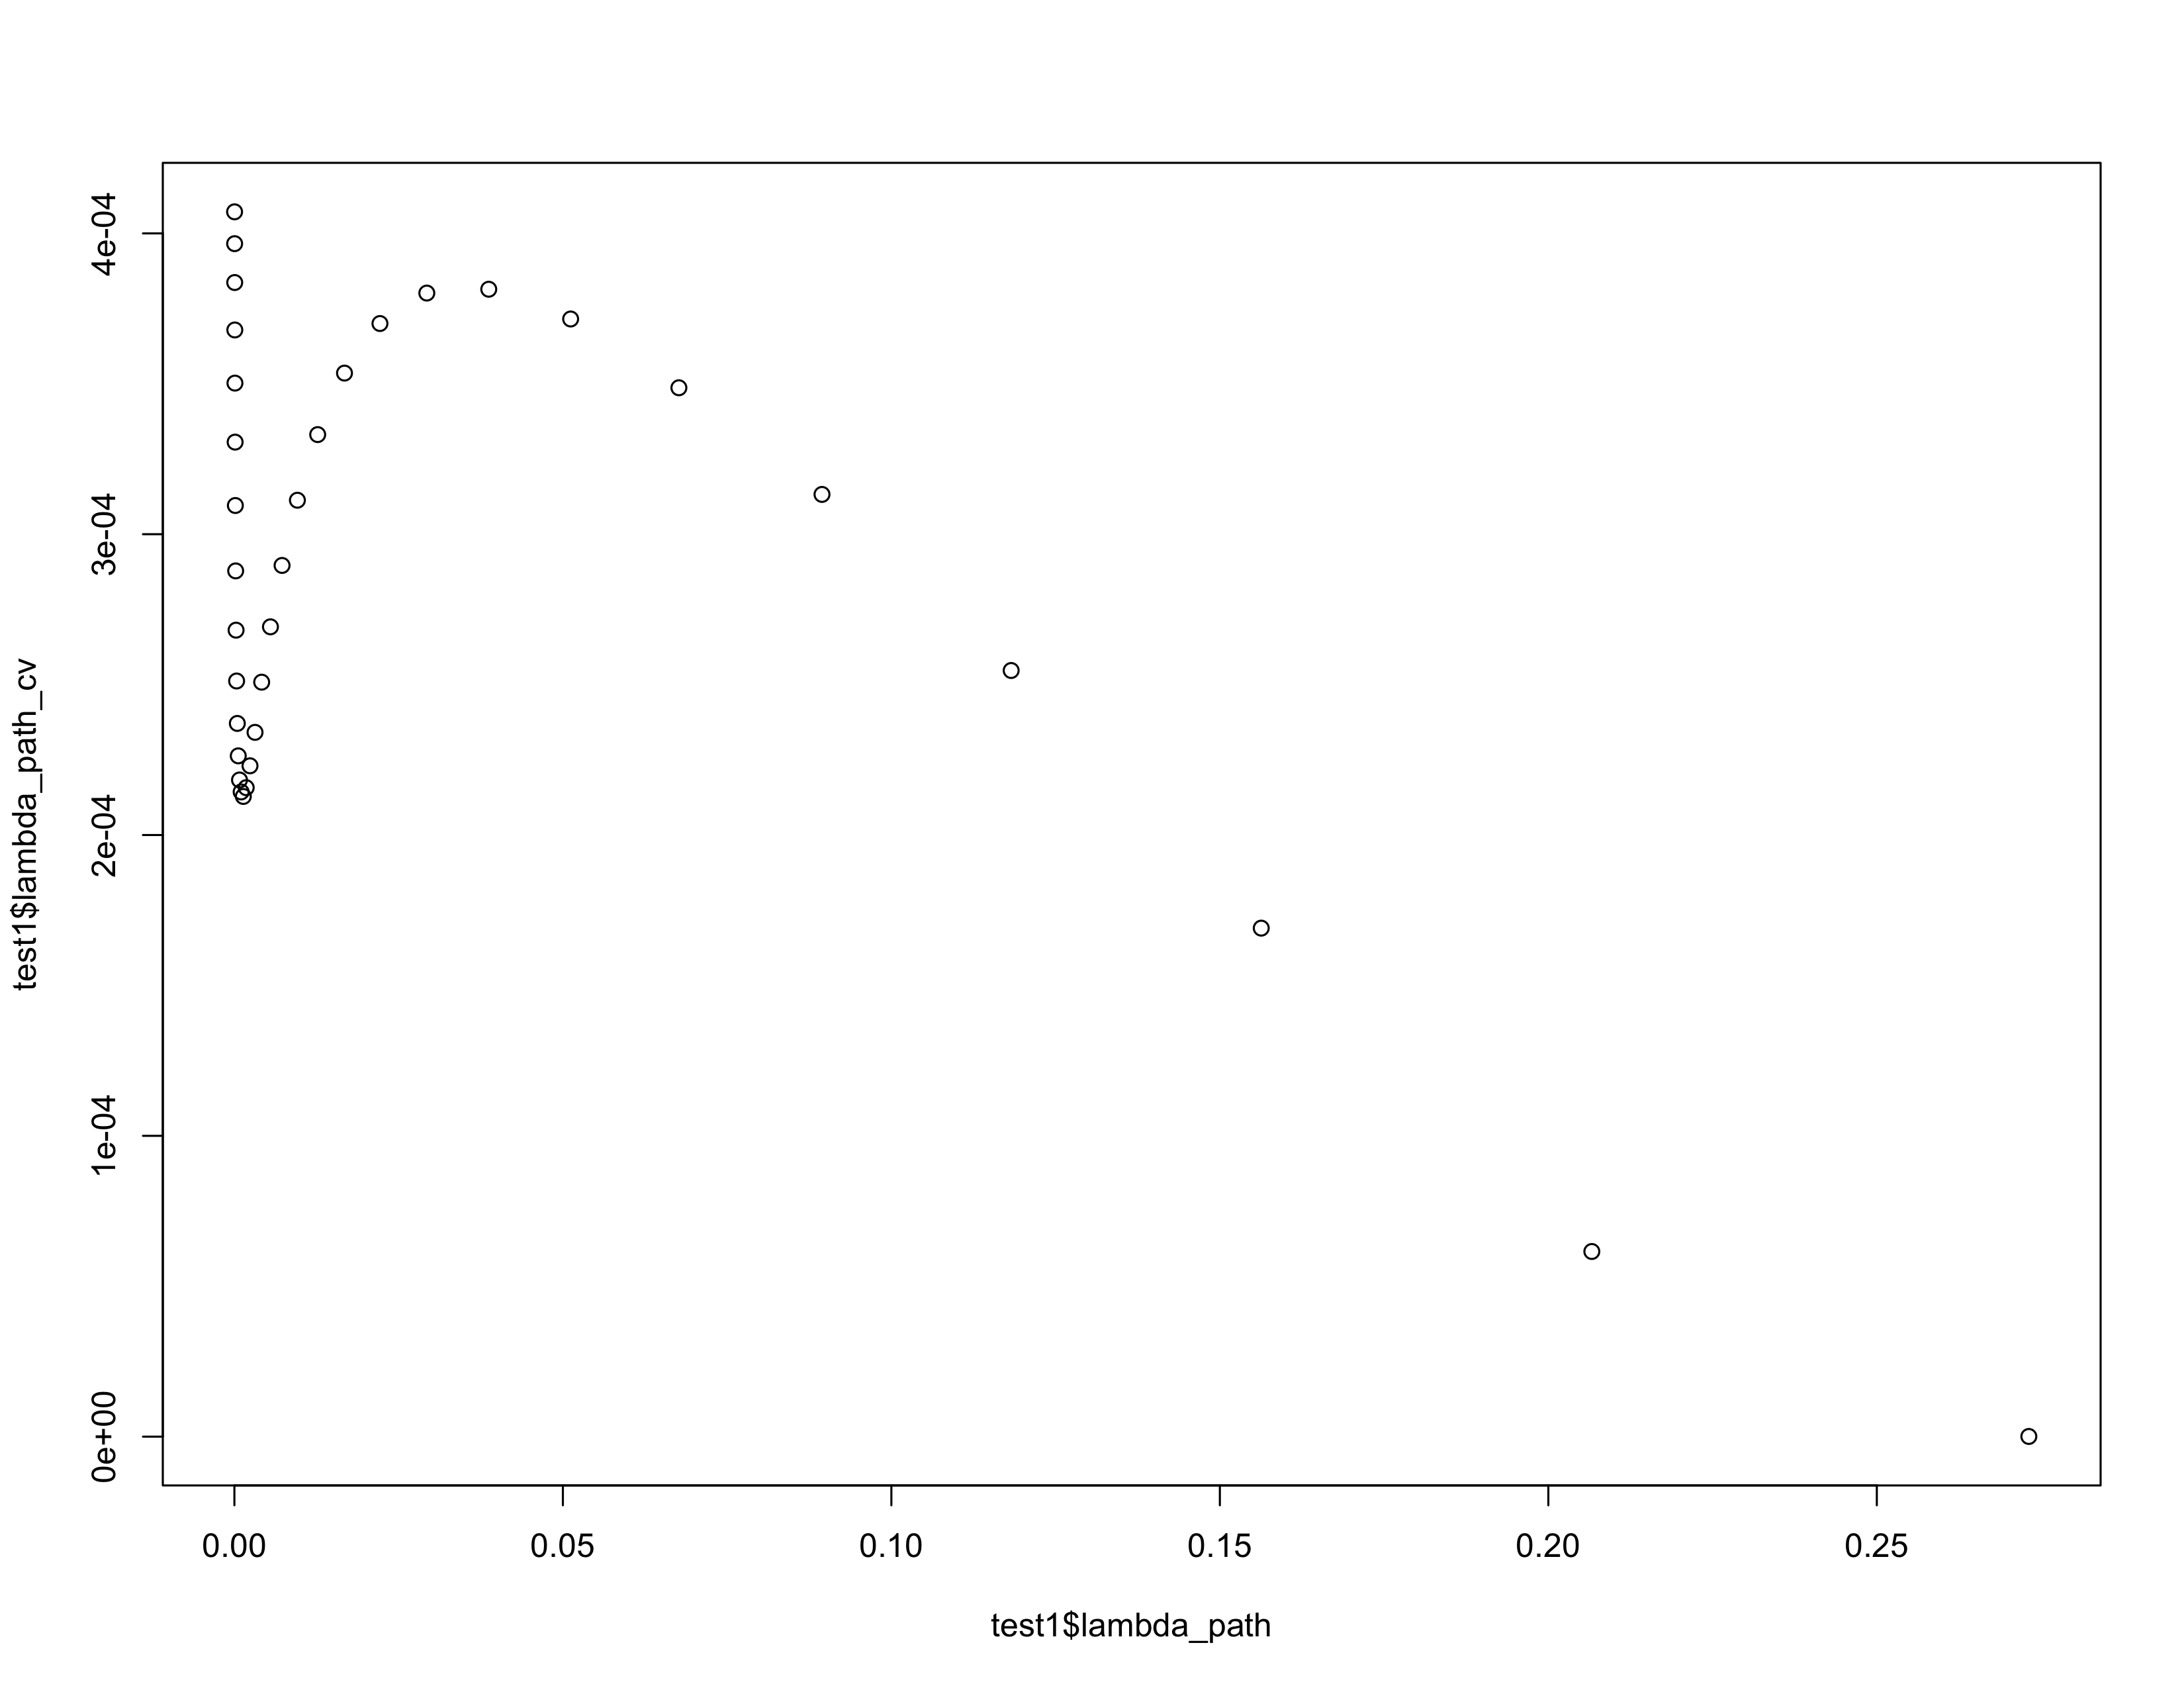
\includegraphics[width=1\linewidth]{./result_plot/cv_square/4wrong_path_plot}
\end{subfigure}

\end{figure}

\begin{figure}[H]
\centering
\begin{subfigure}{0.5\textwidth}
  \centering
  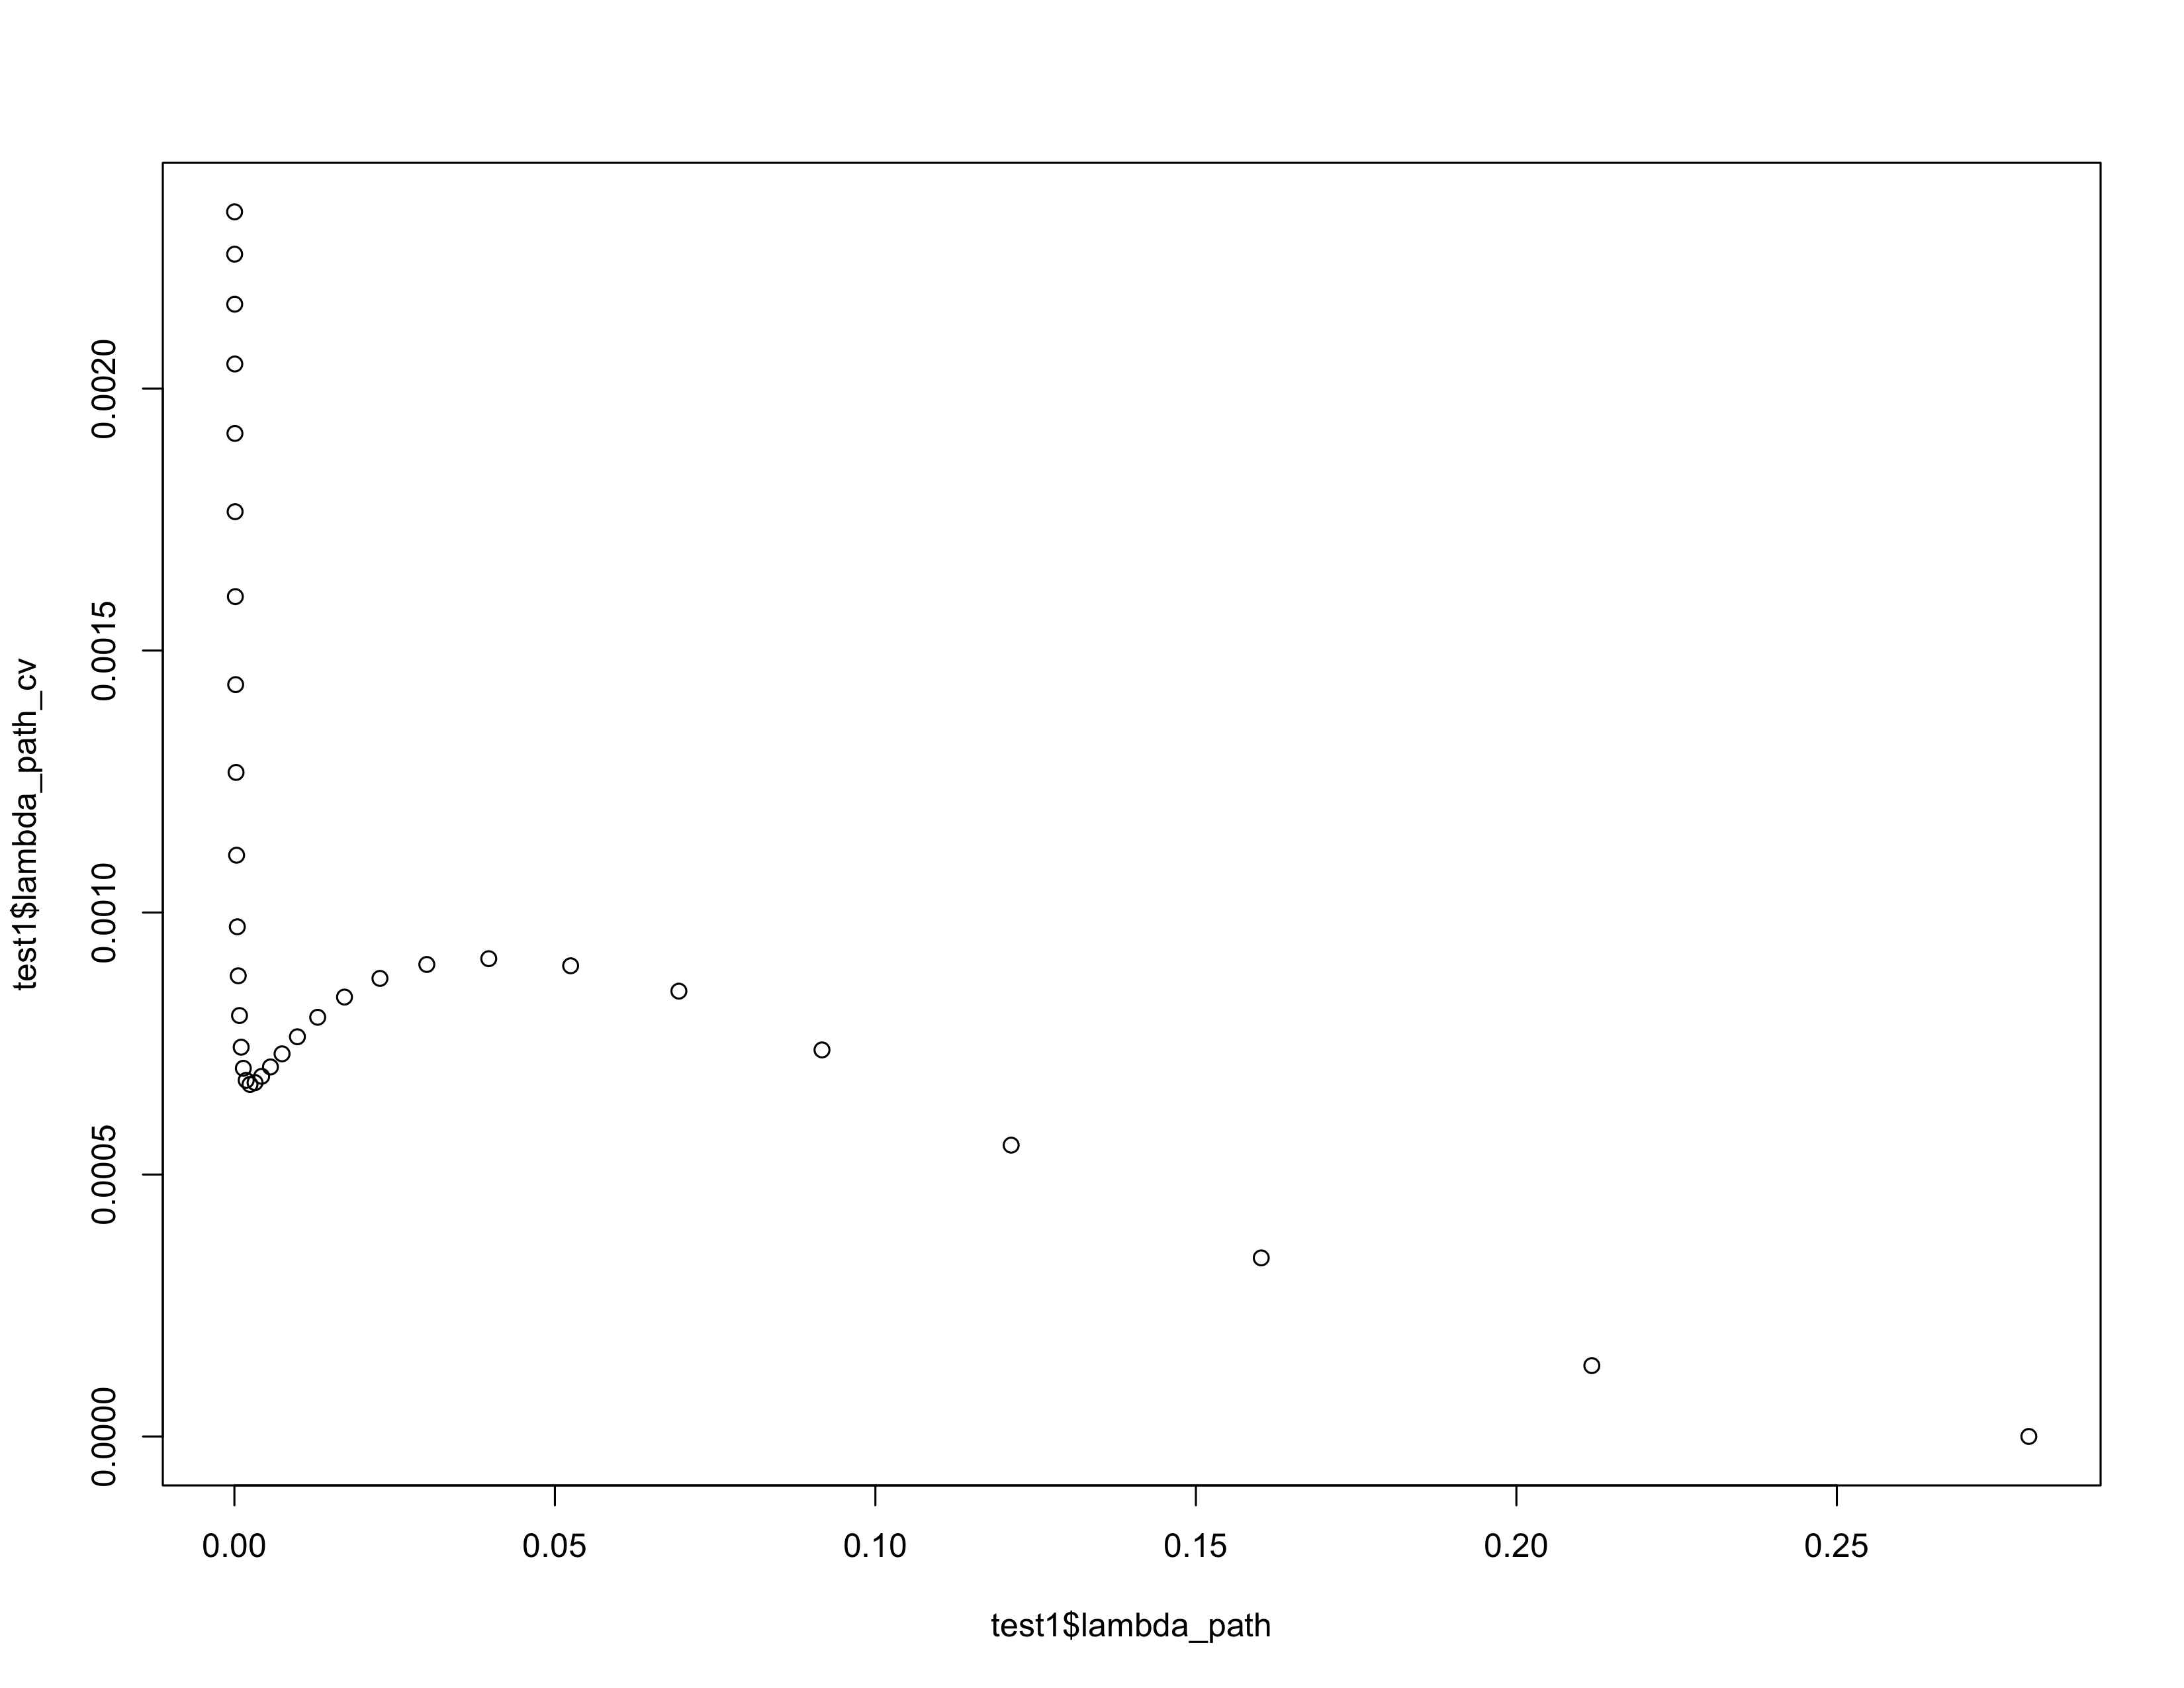
\includegraphics[width=1\linewidth]{./result_plot/cv_square/5wrong_path_plot}
\end{subfigure}%
\begin{subfigure}{.5\textwidth}
  \centering
  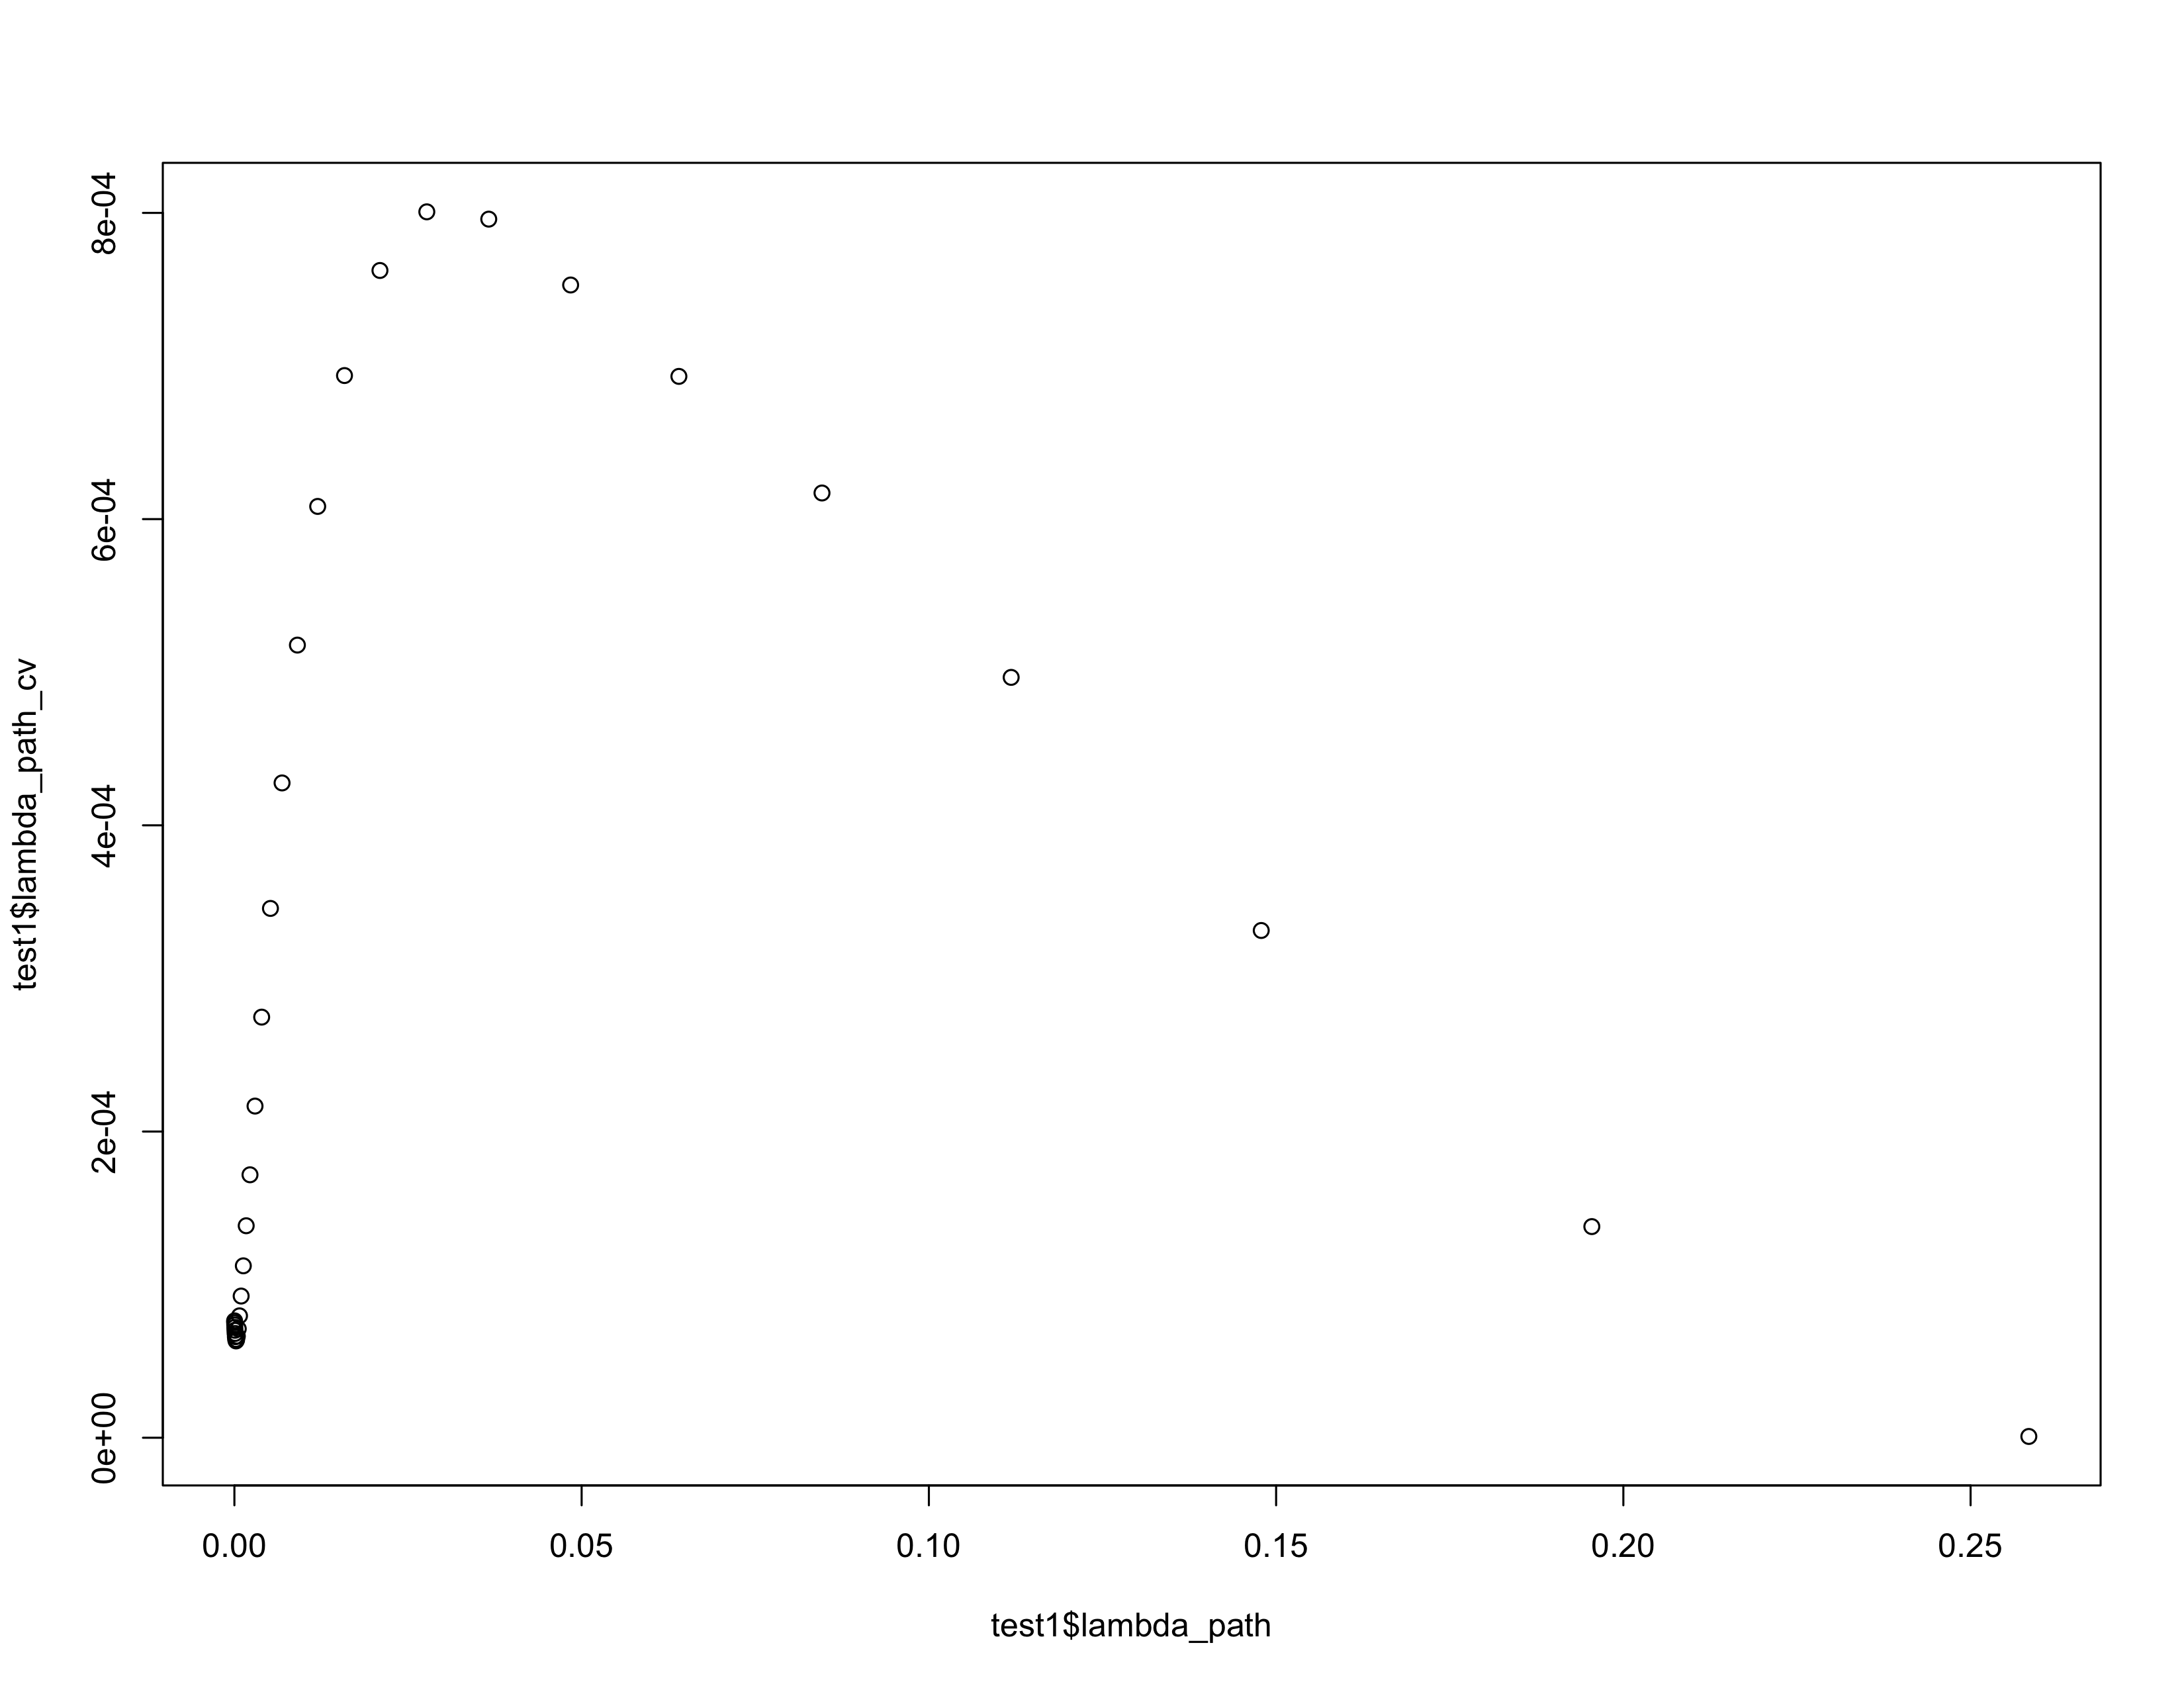
\includegraphics[width=1\linewidth]{./result_plot/cv_square/6wrong_path_plot}
\end{subfigure}

\end{figure}

\begin{figure}[H]
\centering
\begin{subfigure}{0.5\textwidth}
  \centering
  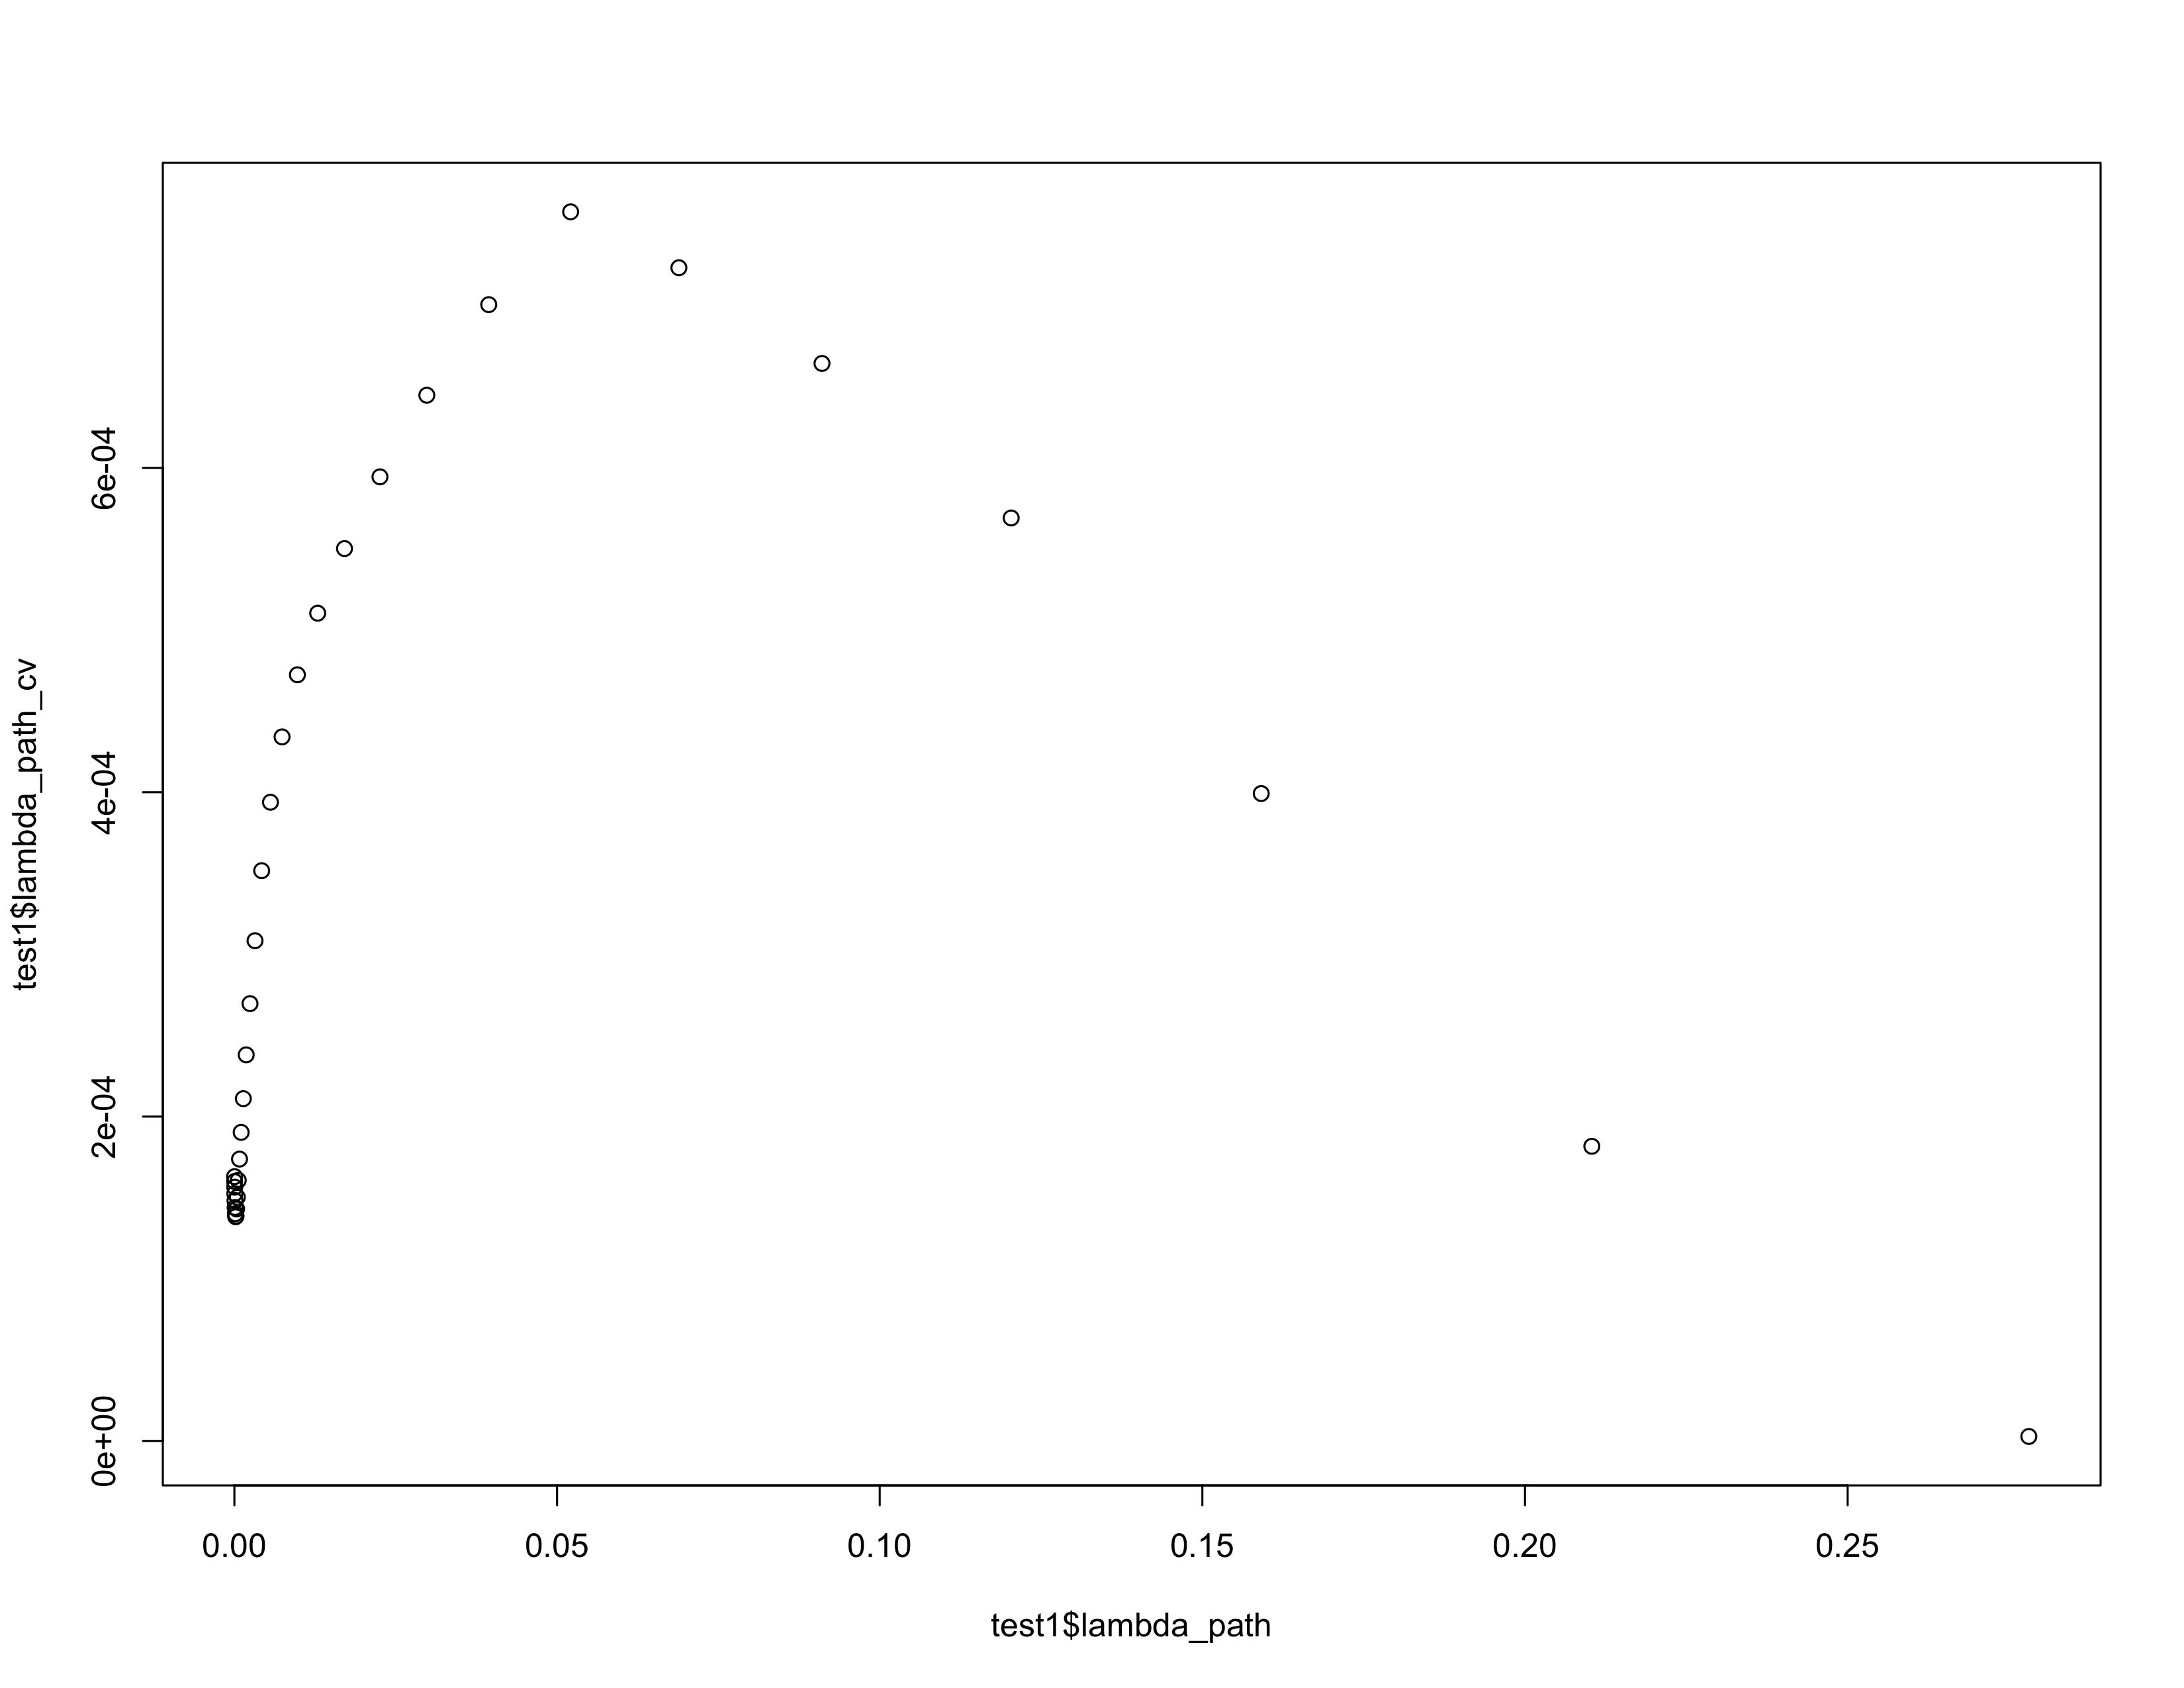
\includegraphics[width=1\linewidth]{./result_plot/cv_square/7wrong_path_plot}
\end{subfigure}%
\begin{subfigure}{.5\textwidth}
  \centering
  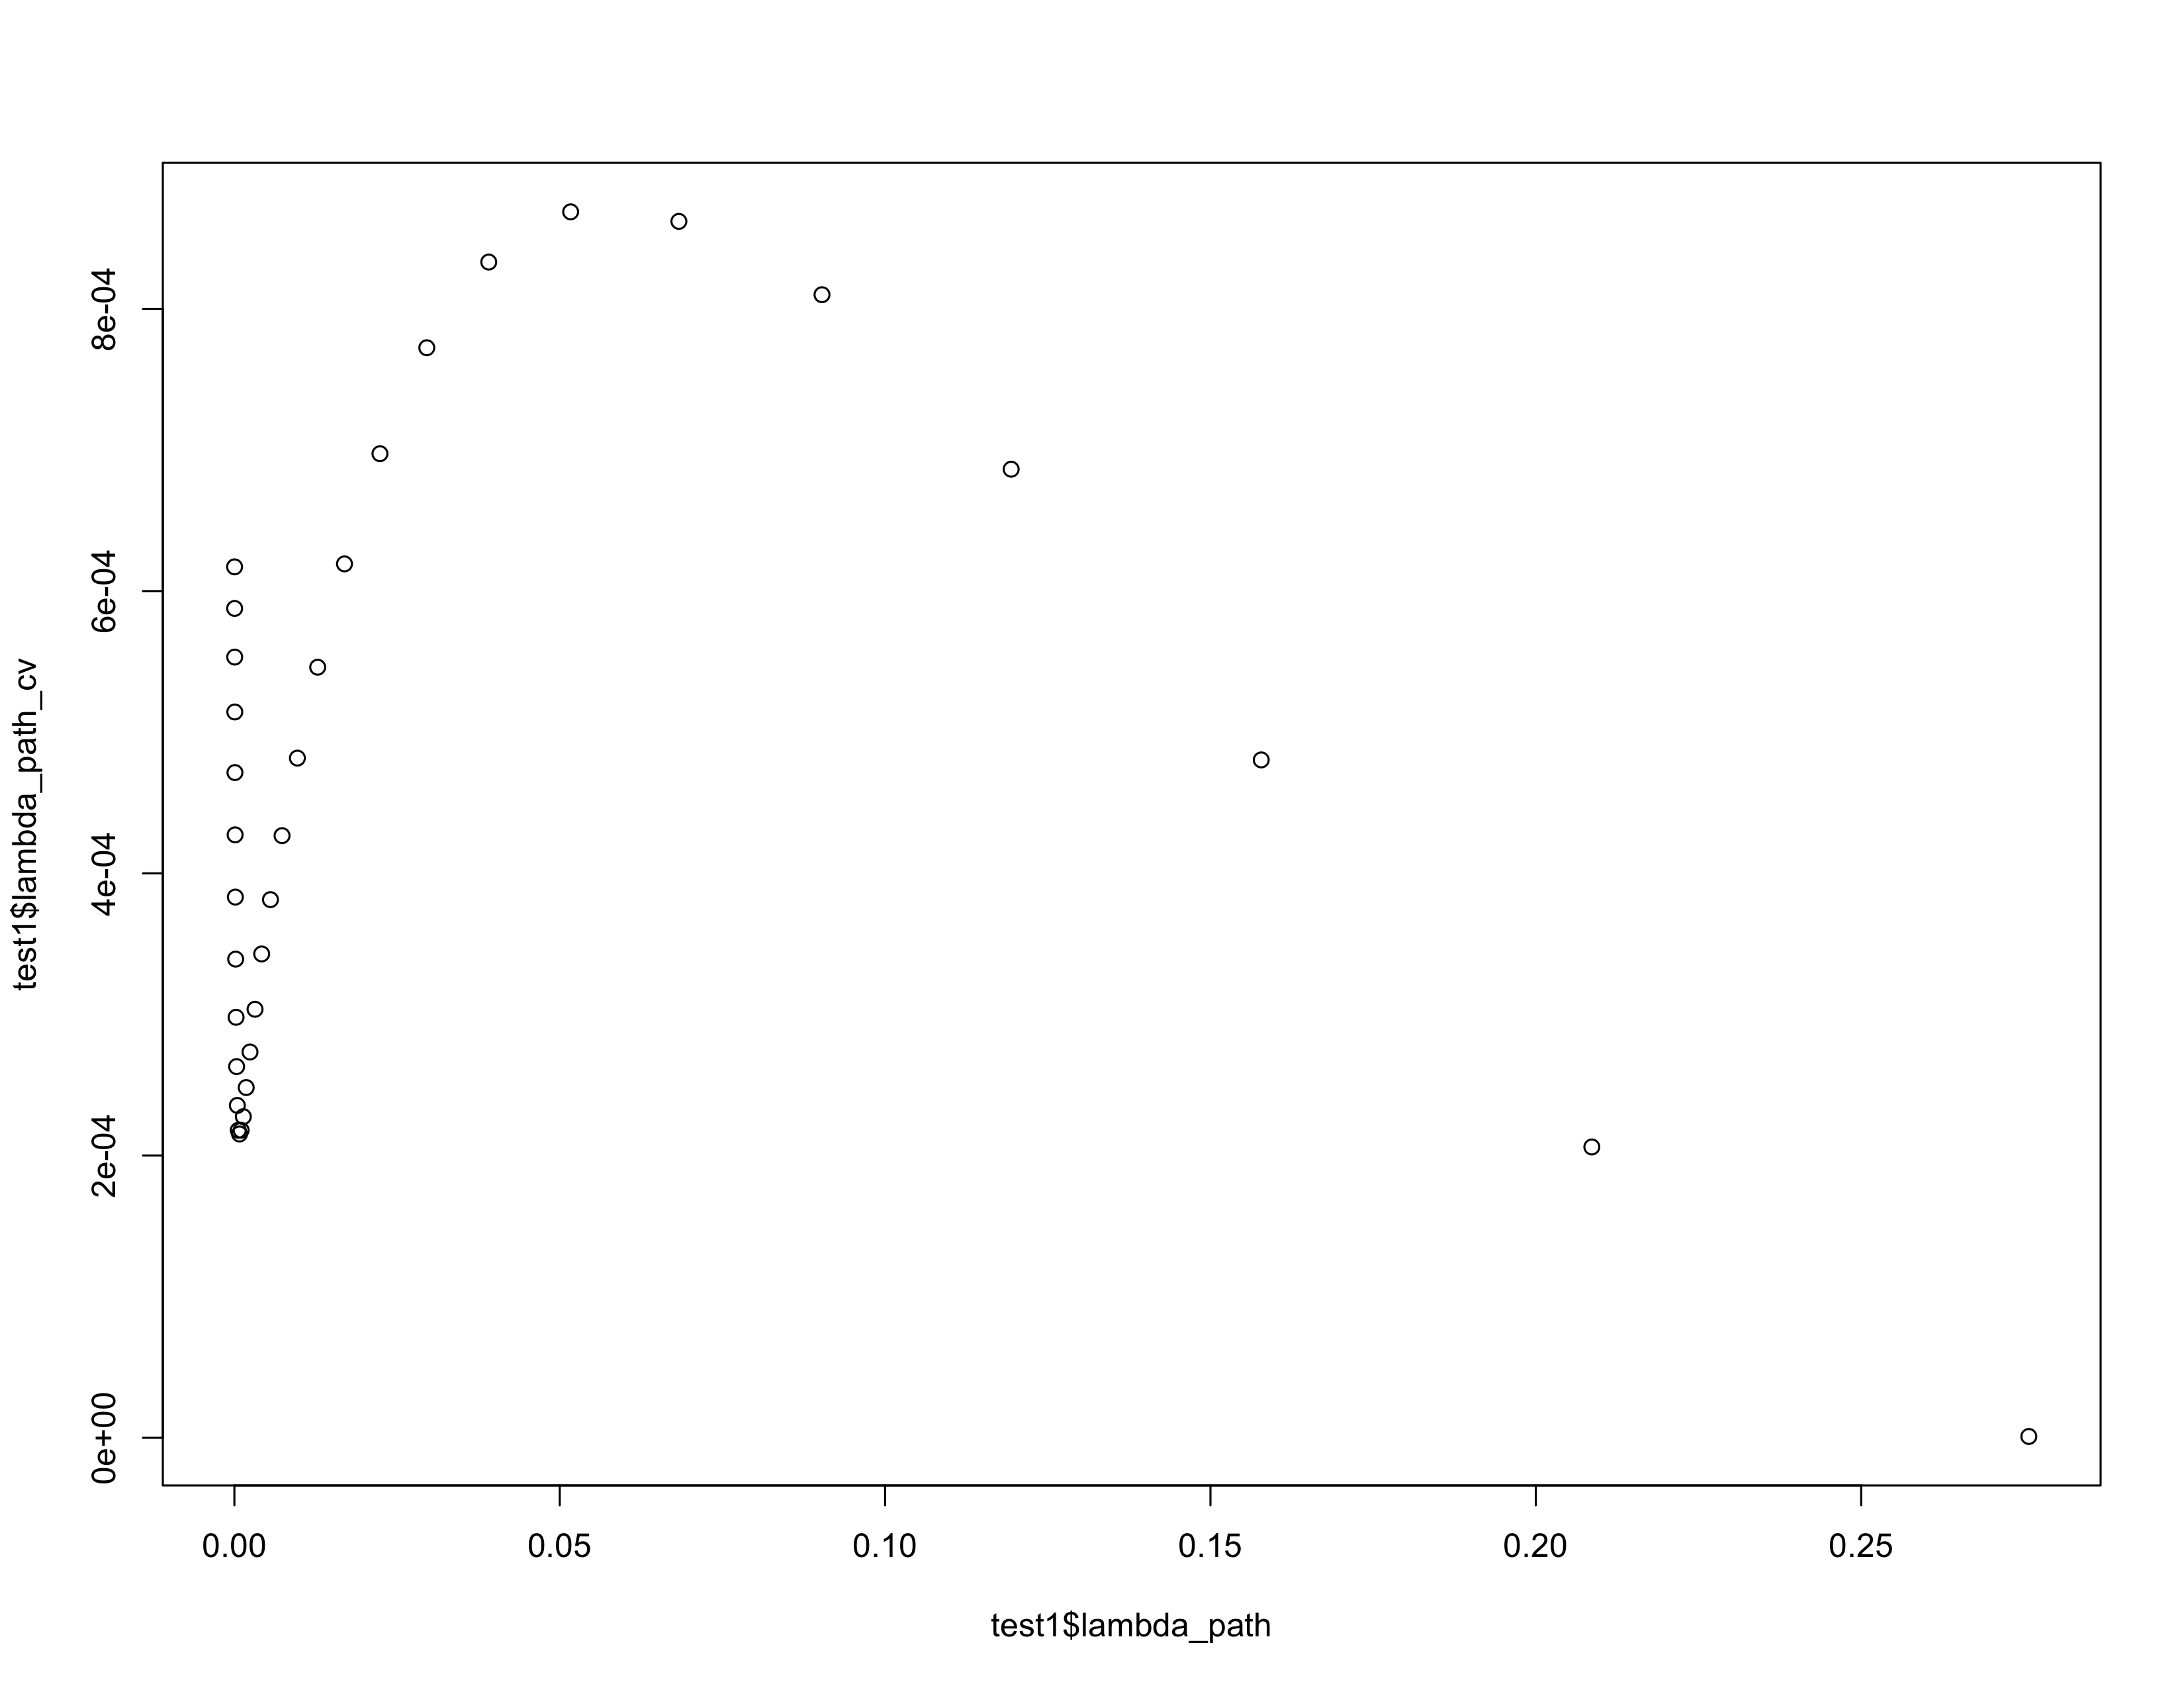
\includegraphics[width=1\linewidth]{./result_plot/cv_square/8wrong_path_plot}
\end{subfigure}

\end{figure}

\begin{figure}[H]
\centering
\begin{subfigure}{0.5\textwidth}
  \centering
  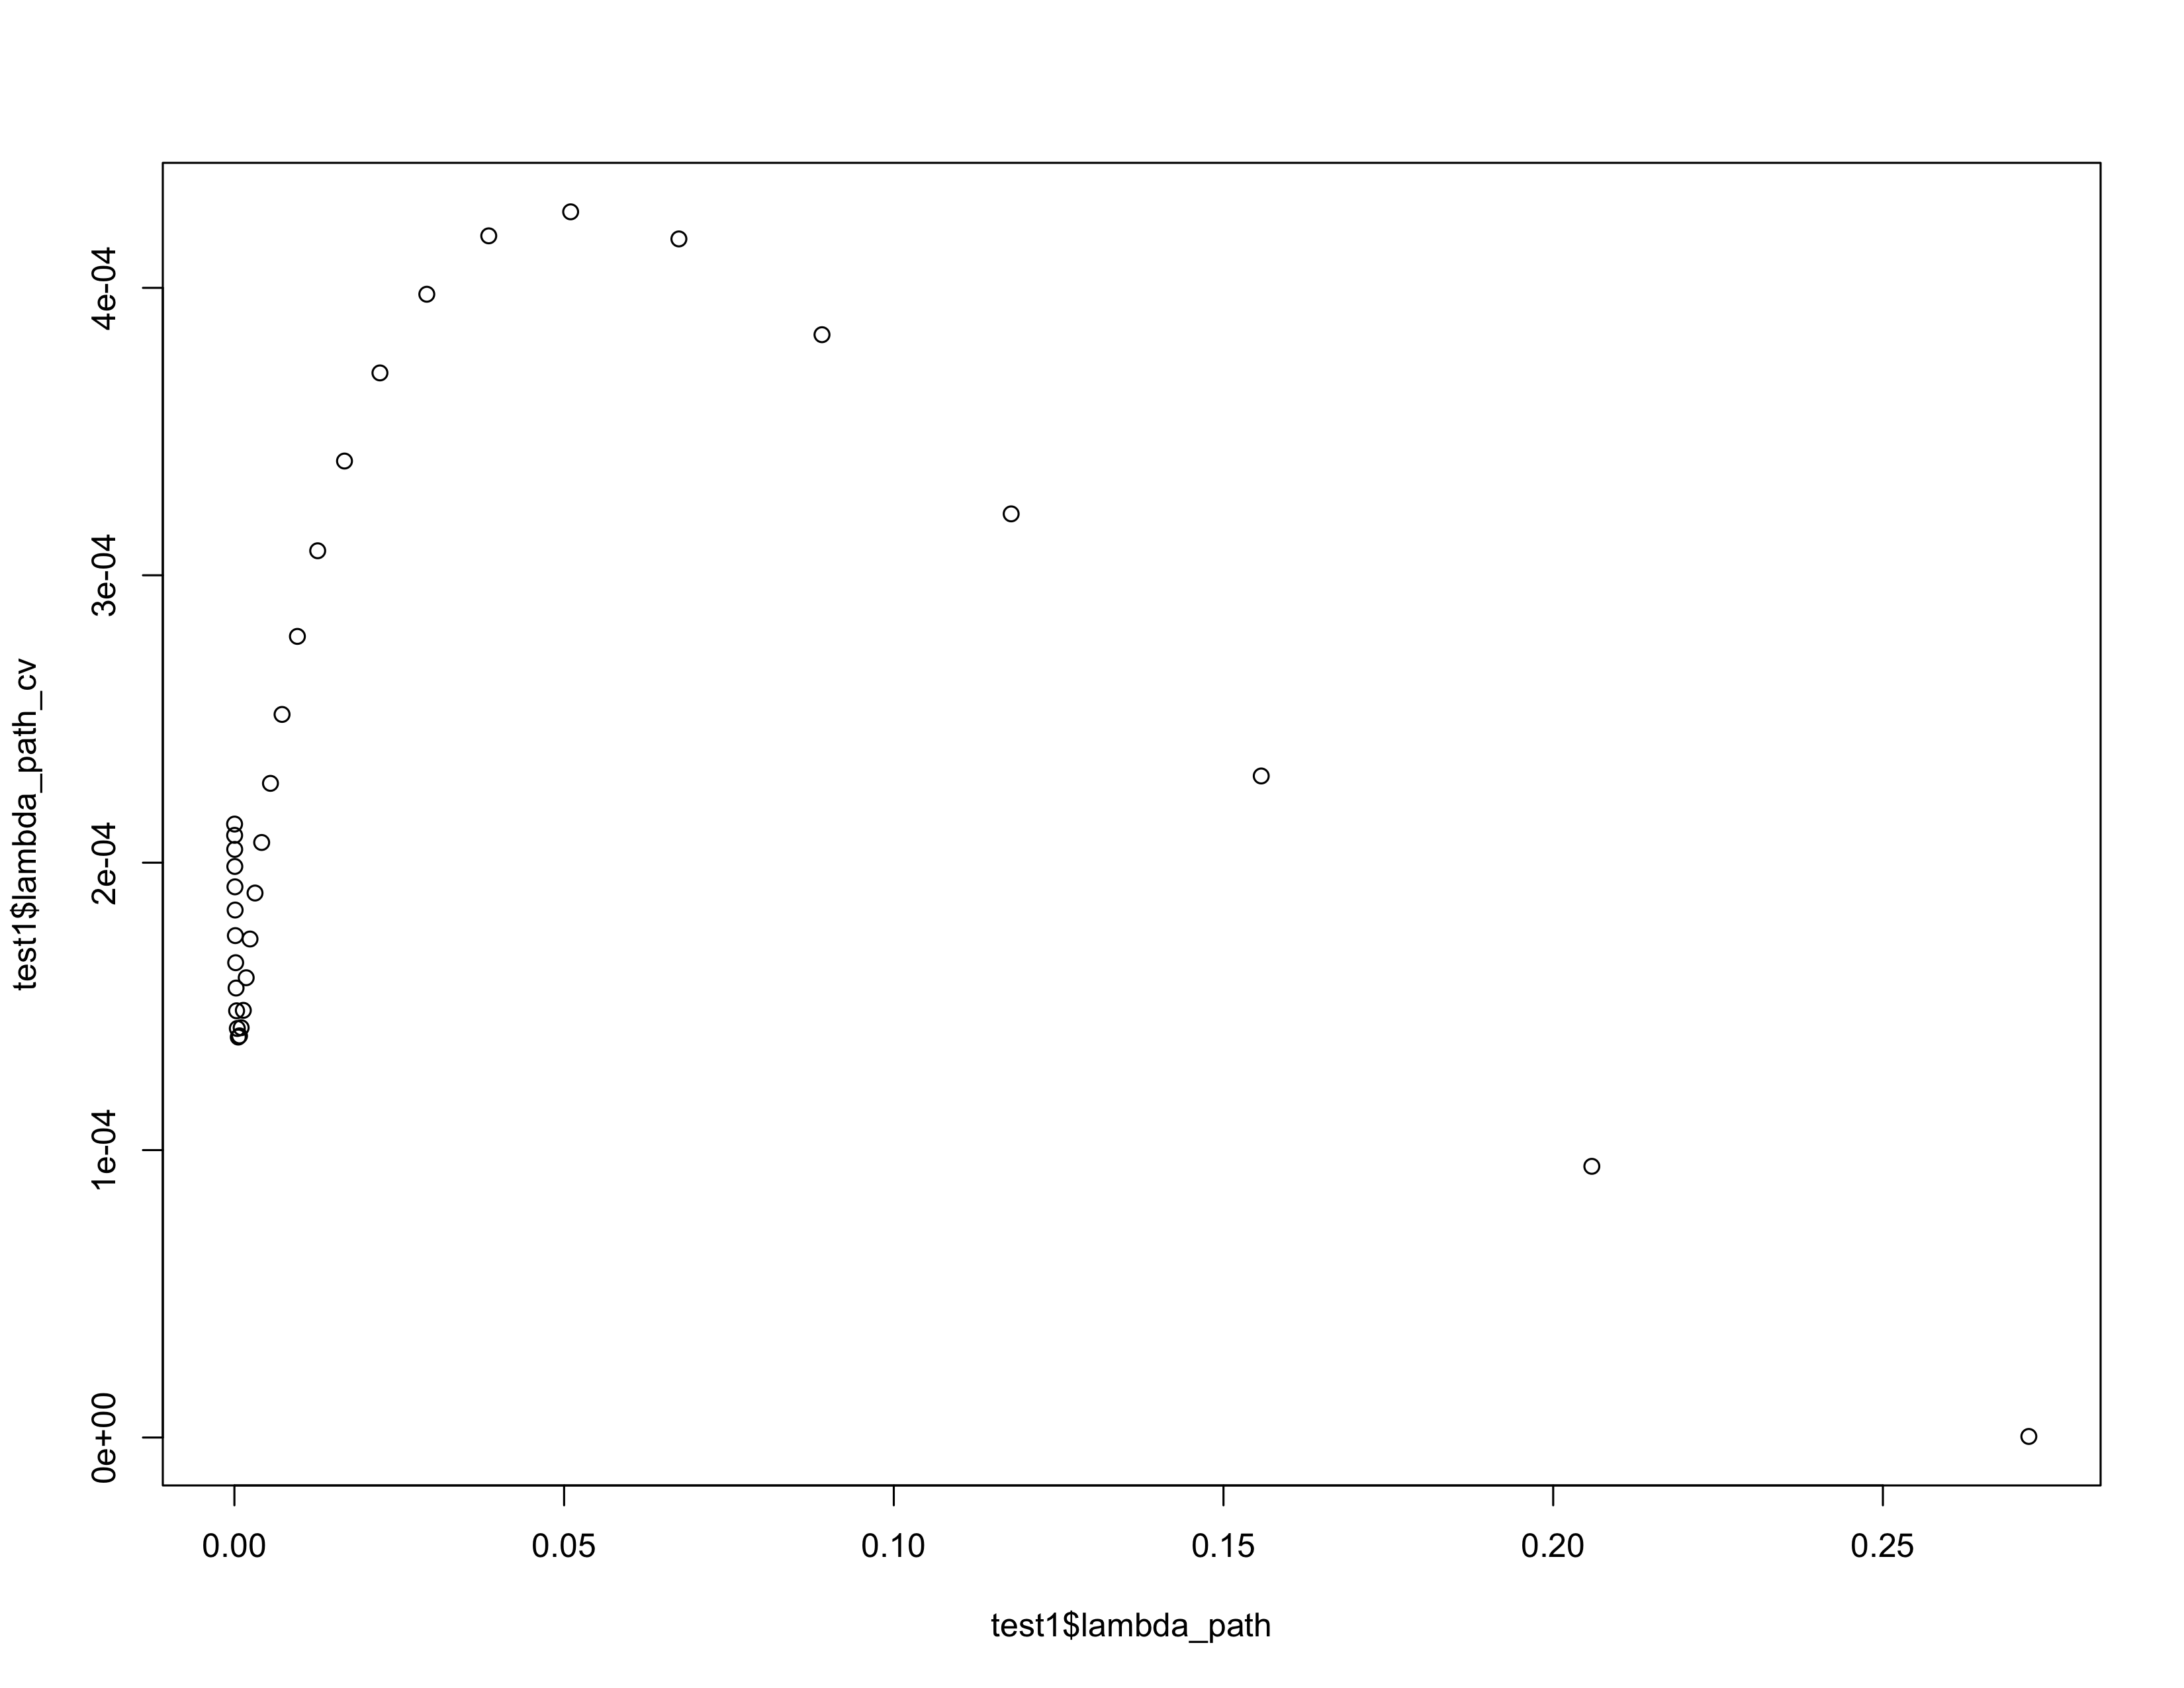
\includegraphics[width=1\linewidth]{./result_plot/cv_square/9wrong_path_plot}
\end{subfigure}%
\begin{subfigure}{.5\textwidth}
  \centering
  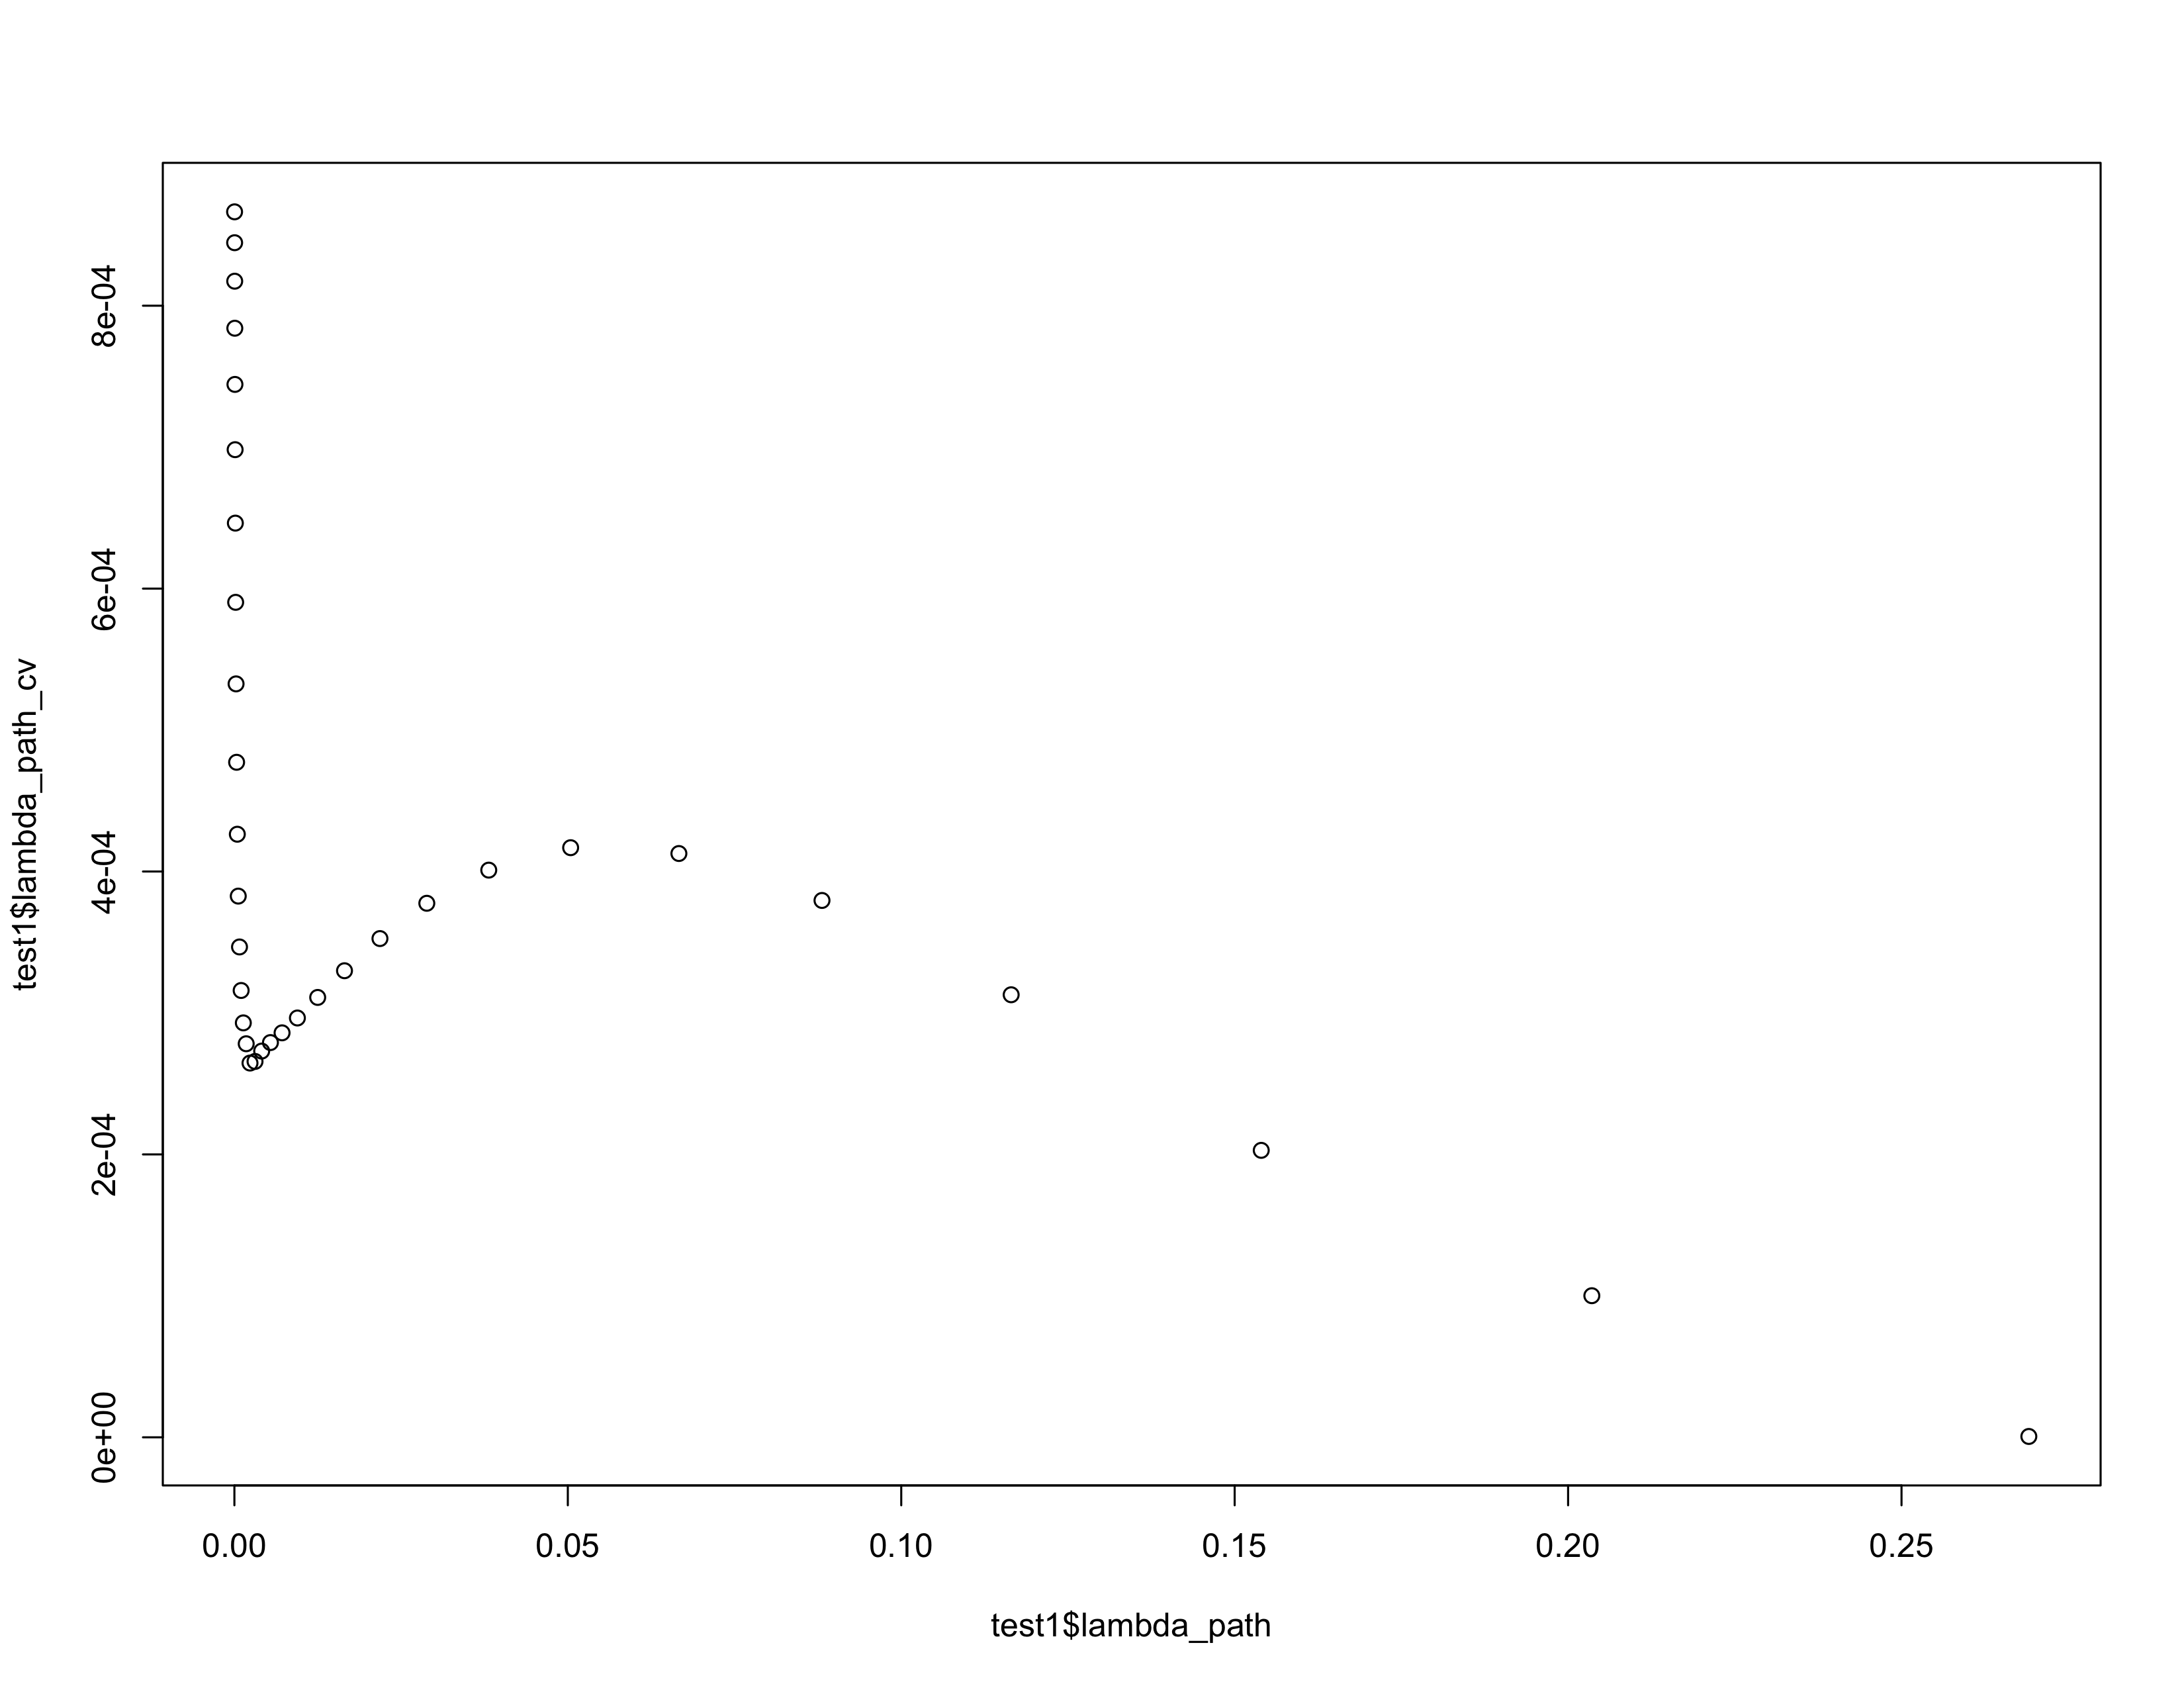
\includegraphics[width=1\linewidth]{./result_plot/cv_square/10wrong_path_plot}
\end{subfigure}

\end{figure}




\end{document}
